\documentclass[twoside]{book}

% Packages required by doxygen
\usepackage{calc}
\usepackage{doxygen}
\usepackage{graphicx}
\usepackage[utf8]{inputenc}
\usepackage{makeidx}
\usepackage{multicol}
\usepackage{multirow}
\usepackage{textcomp}
\usepackage[table]{xcolor}

% Font selection
\usepackage[T1]{fontenc}
\usepackage{mathptmx}
\usepackage[scaled=.90]{helvet}
\usepackage{courier}
\usepackage{amssymb}
\usepackage{sectsty}
\renewcommand{\familydefault}{\sfdefault}
\allsectionsfont{%
  \fontseries{bc}\selectfont%
  \color{darkgray}%
}
\renewcommand{\DoxyLabelFont}{%
  \fontseries{bc}\selectfont%
  \color{darkgray}%
}

% Page & text layout
\usepackage{geometry}
\geometry{%
  a4paper,%
  top=2.5cm,%
  bottom=2.5cm,%
  left=2.5cm,%
  right=2.5cm%
}
\tolerance=750
\hfuzz=15pt
\hbadness=750
\setlength{\emergencystretch}{15pt}
\setlength{\parindent}{0cm}
\setlength{\parskip}{0.2cm}
\makeatletter
\renewcommand{\paragraph}{%
  \@startsection{paragraph}{4}{0ex}{-1.0ex}{1.0ex}{%
    \normalfont\normalsize\bfseries\SS@parafont%
  }%
}
\renewcommand{\subparagraph}{%
  \@startsection{subparagraph}{5}{0ex}{-1.0ex}{1.0ex}{%
    \normalfont\normalsize\bfseries\SS@subparafont%
  }%
}
\makeatother

% Headers & footers
\usepackage{fancyhdr}
\pagestyle{fancyplain}
\fancyhead[LE]{\fancyplain{}{\bfseries\thepage}}
\fancyhead[CE]{\fancyplain{}{}}
\fancyhead[RE]{\fancyplain{}{\bfseries\leftmark}}
\fancyhead[LO]{\fancyplain{}{\bfseries\rightmark}}
\fancyhead[CO]{\fancyplain{}{}}
\fancyhead[RO]{\fancyplain{}{\bfseries\thepage}}
\fancyfoot[LE]{\fancyplain{}{}}
\fancyfoot[CE]{\fancyplain{}{}}
\fancyfoot[RE]{\fancyplain{}{\bfseries\scriptsize Generated on Thu Feb 22 2018 16\-:56\-:02 for Potku by Doxygen }}
\fancyfoot[LO]{\fancyplain{}{\bfseries\scriptsize Generated on Thu Feb 22 2018 16\-:56\-:02 for Potku by Doxygen }}
\fancyfoot[CO]{\fancyplain{}{}}
\fancyfoot[RO]{\fancyplain{}{}}
\renewcommand{\footrulewidth}{0.4pt}
\renewcommand{\chaptermark}[1]{%
  \markboth{#1}{}%
}
\renewcommand{\sectionmark}[1]{%
  \markright{\thesection\ #1}%
}

% Indices & bibliography
\usepackage{natbib}
\usepackage[titles]{tocloft}
\setcounter{tocdepth}{3}
\setcounter{secnumdepth}{5}
\makeindex

% Hyperlinks (required, but should be loaded last)
\usepackage{ifpdf}
\ifpdf
  \usepackage[pdftex,pagebackref=true]{hyperref}
\else
  \usepackage[ps2pdf,pagebackref=true]{hyperref}
\fi
\hypersetup{%
  colorlinks=true,%
  linkcolor=blue,%
  citecolor=blue,%
  unicode%
}

% Custom commands
\newcommand{\clearemptydoublepage}{%
  \newpage{\pagestyle{empty}\cleardoublepage}%
}


%===== C O N T E N T S =====

\begin{document}

% Titlepage & ToC
\hypersetup{pageanchor=false}
\pagenumbering{roman}
\begin{titlepage}
\vspace*{7cm}
\begin{center}%
{\Large Potku \\[1ex]\large 2.\-0.\-0 }\\
\vspace*{1cm}
{\large Generated by Doxygen 1.8.5}\\
\vspace*{0.5cm}
{\small Thu Feb 22 2018 16:56:02}\\
\end{center}
\end{titlepage}
\clearemptydoublepage
\tableofcontents
\clearemptydoublepage
\pagenumbering{arabic}
\hypersetup{pageanchor=true}

%--- Begin generated contents ---
\chapter{Hierarchical Index}
\section{Class Hierarchy}
This inheritance list is sorted roughly, but not completely, alphabetically\-:\begin{DoxyCompactList}
\item \contentsline{section}{Widgets.\-Matplotlib\-Depth\-Profile\-Widget.\-Matplotlib\-Depth\-Profile\-Widget.\-\_\-\-\_\-limit}{\pageref{classWidgets_1_1MatplotlibDepthProfileWidget_1_1MatplotlibDepthProfileWidget_1_1____limit}}{}
\item \contentsline{section}{Modules.\-Selection.\-Axes\-Limits}{\pageref{classModules_1_1Selection_1_1AxesLimits}}{}
\item \contentsline{section}{Modules.\-Calibration\-Parameters.\-Calibration\-Parameters}{\pageref{classModules_1_1CalibrationParameters_1_1CalibrationParameters}}{}
\item \contentsline{section}{Dialogs.\-Import\-Measurement\-Dialog.\-Coinc\-Timing}{\pageref{classDialogs_1_1ImportMeasurementDialog_1_1CoincTiming}}{}
\item \contentsline{section}{Modules.\-Cut\-File.\-Cut\-File}{\pageref{classModules_1_1CutFile_1_1CutFile}}{}
\item \contentsline{section}{Modules.\-Depth\-Profile\-Settings.\-Depth\-Profile\-Settings}{\pageref{classModules_1_1DepthProfileSettings_1_1DepthProfileSettings}}{}
\item \contentsline{section}{Modules.\-Element.\-Element}{\pageref{classModules_1_1Element_1_1Element}}{}
\item \contentsline{section}{Modules.\-Element\-Losses.\-Element\-Losses}{\pageref{classModules_1_1ElementLosses_1_1ElementLosses}}{}
\item \contentsline{section}{Modules.\-Element\-Losses.\-Element\-Losses\-Split\-Holder}{\pageref{classModules_1_1ElementLosses_1_1ElementLossesSplitHolder}}{}
\item \contentsline{section}{Modules.\-Energy\-Spectrum.\-Energy\-Spectrum}{\pageref{classModules_1_1EnergySpectrum_1_1EnergySpectrum}}{}
\item \contentsline{section}{Modules.\-Global\-Settings.\-Global\-Settings}{\pageref{classModules_1_1GlobalSettings_1_1GlobalSettings}}{}
\item Handler\begin{DoxyCompactList}
\item \contentsline{section}{Modules.\-Ui\-Log\-Handlers.\-custom\-Log\-Handler}{\pageref{classModules_1_1UiLogHandlers_1_1customLogHandler}}{}
\end{DoxyCompactList}
\item \contentsline{section}{Modules.\-Icon\-Manager.\-Icon\-Manager}{\pageref{classModules_1_1IconManager_1_1IconManager}}{}
\item \contentsline{section}{Modules.\-Element.\-Isotope}{\pageref{classModules_1_1Element_1_1Isotope}}{}
\item \contentsline{section}{Modules.\-Masses.\-Masses}{\pageref{classModules_1_1Masses_1_1Masses}}{}
\item \contentsline{section}{Modules.\-Measurement.\-Measurement}{\pageref{classModules_1_1Measurement_1_1Measurement}}{}
\item \contentsline{section}{Modules.\-Measurement.\-Measurements}{\pageref{classModules_1_1Measurement_1_1Measurements}}{}
\item \contentsline{section}{Modules.\-Measuring\-Settings.\-Measuring\-Settings}{\pageref{classModules_1_1MeasuringSettings_1_1MeasuringSettings}}{}
\item \contentsline{section}{Widgets.\-Matplotlib\-Widget.\-Mock\-Manager}{\pageref{classWidgets_1_1MatplotlibWidget_1_1MockManager}}{}
\item Navigation\-Toolbar\begin{DoxyCompactList}
\item \contentsline{section}{Modules.\-Navigation\-Tool\-Bar2\-Q\-T\-View.\-Navigation\-Tool\-Bar2\-Q\-T\-View}{\pageref{classModules_1_1NavigationToolBar2QTView_1_1NavigationToolBar2QTView}}{}
\end{DoxyCompactList}
\item \contentsline{section}{Modules.\-Null.\-Null}{\pageref{classModules_1_1Null_1_1Null}}{}
\item object\begin{DoxyCompactList}
\item \contentsline{section}{Modules.\-Depth\-Files.\-Depth\-Files}{\pageref{classModules_1_1DepthFiles_1_1DepthFiles}}{}
\end{DoxyCompactList}
\item \contentsline{section}{Modules.\-Project.\-Project}{\pageref{classModules_1_1Project_1_1Project}}{}
\item Q\-Dialog\begin{DoxyCompactList}
\item \contentsline{section}{Dialogs.\-About\-Dialog.\-About\-Dialog}{\pageref{classDialogs_1_1AboutDialog_1_1AboutDialog}}{}
\item \contentsline{section}{Dialogs.\-Calibration\-Dialog.\-Calibration\-Dialog}{\pageref{classDialogs_1_1CalibrationDialog_1_1CalibrationDialog}}{}
\item \contentsline{section}{Dialogs.\-Depth\-Profile\-Dialog.\-Depth\-Profile\-Dialog}{\pageref{classDialogs_1_1DepthProfileDialog_1_1DepthProfileDialog}}{}
\item \contentsline{section}{Dialogs.\-Depth\-Profile\-Ignore\-Elements.\-Depth\-Profile\-Ignore\-Elements}{\pageref{classDialogs_1_1DepthProfileIgnoreElements_1_1DepthProfileIgnoreElements}}{}
\item \contentsline{section}{Dialogs.\-Element\-Losses\-Dialog.\-Element\-Losses\-Dialog}{\pageref{classDialogs_1_1ElementLossesDialog_1_1ElementLossesDialog}}{}
\item \contentsline{section}{Dialogs.\-Element\-Selection\-Dialog.\-Element\-Selection\-Dialog}{\pageref{classDialogs_1_1ElementSelectionDialog_1_1ElementSelectionDialog}}{}
\item \contentsline{section}{Dialogs.\-Energy\-Spectrum\-Dialog.\-Energy\-Spectrum\-Params\-Dialog}{\pageref{classDialogs_1_1EnergySpectrumDialog_1_1EnergySpectrumParamsDialog}}{}
\item \contentsline{section}{Dialogs.\-Global\-Settings\-Dialog.\-Global\-Settings\-Dialog}{\pageref{classDialogs_1_1GlobalSettingsDialog_1_1GlobalSettingsDialog}}{}
\item \contentsline{section}{Dialogs.\-Graph\-Ignore\-Elements.\-Graph\-Ignore\-Elements}{\pageref{classDialogs_1_1GraphIgnoreElements_1_1GraphIgnoreElements}}{}
\item \contentsline{section}{Dialogs.\-Graph\-Settings\-Dialog.\-Tofe\-Graph\-Settings\-Widget}{\pageref{classDialogs_1_1GraphSettingsDialog_1_1TofeGraphSettingsWidget}}{}
\item \contentsline{section}{Dialogs.\-Import\-Measurement\-Binary.\-Import\-Dialog\-Binary}{\pageref{classDialogs_1_1ImportMeasurementBinary_1_1ImportDialogBinary}}{}
\item \contentsline{section}{Dialogs.\-Import\-Measurement\-Dialog.\-Import\-Measurements\-Dialog}{\pageref{classDialogs_1_1ImportMeasurementDialog_1_1ImportMeasurementsDialog}}{}
\item \contentsline{section}{Dialogs.\-Import\-Timing\-Graph\-Dialog.\-Import\-Timing\-Graph\-Dialog}{\pageref{classDialogs_1_1ImportTimingGraphDialog_1_1ImportTimingGraphDialog}}{}
\item \contentsline{section}{Dialogs.\-Measurement\-Settings\-Dialogs.\-Calibration\-Settings}{\pageref{classDialogs_1_1MeasurementSettingsDialogs_1_1CalibrationSettings}}{}
\item \contentsline{section}{Dialogs.\-Measurement\-Settings\-Dialogs.\-Depth\-Profile\-Settings}{\pageref{classDialogs_1_1MeasurementSettingsDialogs_1_1DepthProfileSettings}}{}
\item \contentsline{section}{Dialogs.\-Measurement\-Settings\-Dialogs.\-Measurement\-Unit\-Settings}{\pageref{classDialogs_1_1MeasurementSettingsDialogs_1_1MeasurementUnitSettings}}{}
\item \contentsline{section}{Dialogs.\-Measuring\-Settings\-Dialog.\-Project\-Settings\-Dialog}{\pageref{classDialogs_1_1MeasuringSettingsDialog_1_1ProjectSettingsDialog}}{}
\item \contentsline{section}{Dialogs.\-Project\-New\-Dialog.\-Project\-New\-Dialog}{\pageref{classDialogs_1_1ProjectNewDialog_1_1ProjectNewDialog}}{}
\item \contentsline{section}{Dialogs.\-Selection\-Dialog.\-Selection\-Settings\-Dialog}{\pageref{classDialogs_1_1SelectionDialog_1_1SelectionSettingsDialog}}{}
\end{DoxyCompactList}
\item Q\-Main\-Window\begin{DoxyCompactList}
\item \contentsline{section}{potku.\-Potku}{\pageref{classpotku_1_1Potku}}{}
\end{DoxyCompactList}
\item Q\-Widget\begin{DoxyCompactList}
\item \contentsline{section}{Dialogs.\-Calibration\-Dialog.\-Calibration\-Curve\-Fitting\-Widget}{\pageref{classDialogs_1_1CalibrationDialog_1_1CalibrationCurveFittingWidget}}{}
\item \contentsline{section}{Dialogs.\-Calibration\-Dialog.\-Calibration\-Linear\-Fitting\-Widget}{\pageref{classDialogs_1_1CalibrationDialog_1_1CalibrationLinearFittingWidget}}{}
\item \contentsline{section}{Dialogs.\-Depth\-Profile\-Dialog.\-Depth\-Profile\-Widget}{\pageref{classDialogs_1_1DepthProfileDialog_1_1DepthProfileWidget}}{}
\item \contentsline{section}{Dialogs.\-Element\-Losses\-Dialog.\-Element\-Losses\-Widget}{\pageref{classDialogs_1_1ElementLossesDialog_1_1ElementLossesWidget}}{}
\item \contentsline{section}{Dialogs.\-Energy\-Spectrum\-Dialog.\-Energy\-Spectrum\-Widget}{\pageref{classDialogs_1_1EnergySpectrumDialog_1_1EnergySpectrumWidget}}{}
\item \contentsline{section}{Widgets.\-Log\-Widget.\-Log\-Widget}{\pageref{classWidgets_1_1LogWidget_1_1LogWidget}}{}
\item \contentsline{section}{Widgets.\-Matplotlib\-Widget.\-Matplotlib\-Widget}{\pageref{classWidgets_1_1MatplotlibWidget_1_1MatplotlibWidget}}{}
\begin{DoxyCompactList}
\item \contentsline{section}{Widgets.\-Matplotlib\-Calibration\-Curve\-Fitting\-Widget.\-Matplotlib\-Calibration\-Curve\-Fitting\-Widget}{\pageref{classWidgets_1_1MatplotlibCalibrationCurveFittingWidget_1_1MatplotlibCalibrationCurveFittingWidget}}{}
\item \contentsline{section}{Widgets.\-Matplotlib\-Calibration\-Linear\-Fitting\-Widget.\-Matplotlib\-Calibration\-Linear\-Fitting\-Widget}{\pageref{classWidgets_1_1MatplotlibCalibrationLinearFittingWidget_1_1MatplotlibCalibrationLinearFittingWidget}}{}
\item \contentsline{section}{Widgets.\-Matplotlib\-Depth\-Profile\-Widget.\-Matplotlib\-Depth\-Profile\-Widget}{\pageref{classWidgets_1_1MatplotlibDepthProfileWidget_1_1MatplotlibDepthProfileWidget}}{}
\item \contentsline{section}{Widgets.\-Matplotlib\-Element\-Losses\-Widget.\-Matplotlib\-Element\-Losses\-Widget}{\pageref{classWidgets_1_1MatplotlibElementLossesWidget_1_1MatplotlibElementLossesWidget}}{}
\item \contentsline{section}{Widgets.\-Matplotlib\-Energy\-Spectrum\-Widget.\-Matplotlib\-Energy\-Spectrum\-Widget}{\pageref{classWidgets_1_1MatplotlibEnergySpectrumWidget_1_1MatplotlibEnergySpectrumWidget}}{}
\item \contentsline{section}{Widgets.\-Matplotlib\-Import\-Timing\-Widget.\-Matplotlib\-Import\-Timing\-Widget}{\pageref{classWidgets_1_1MatplotlibImportTimingWidget_1_1MatplotlibImportTimingWidget}}{}
\item \contentsline{section}{Widgets.\-Matplotlib\-Tofe\-Histogram\-Widget.\-Matplotlib\-Histogram\-Widget}{\pageref{classWidgets_1_1MatplotlibTofeHistogramWidget_1_1MatplotlibHistogramWidget}}{}
\end{DoxyCompactList}
\item \contentsline{section}{Widgets.\-Measurement\-Info\-Widget.\-Measurement\-Info\-Widget}{\pageref{classWidgets_1_1MeasurementInfoWidget_1_1MeasurementInfoWidget}}{}
\item \contentsline{section}{Widgets.\-Measurement\-Tab\-Widget.\-Measurement\-Tab\-Widget}{\pageref{classWidgets_1_1MeasurementTabWidget_1_1MeasurementTabWidget}}{}
\item \contentsline{section}{Widgets.\-Tofe\-Histogram\-Widget.\-Tofe\-Histogram\-Widget}{\pageref{classWidgets_1_1TofeHistogramWidget_1_1TofeHistogramWidget}}{}
\end{DoxyCompactList}
\item \contentsline{section}{Modules.\-Selection.\-Selection}{\pageref{classModules_1_1Selection_1_1Selection}}{}
\item \contentsline{section}{Modules.\-Selection.\-Selector}{\pageref{classModules_1_1Selection_1_1Selector}}{}
\item \contentsline{section}{Modules.\-Settings.\-Settings}{\pageref{classModules_1_1Settings_1_1Settings}}{}
\item \contentsline{section}{Modules.\-Calibration.\-T\-O\-F\-Calibration}{\pageref{classModules_1_1Calibration_1_1TOFCalibration}}{}
\item \contentsline{section}{Modules.\-Calibration.\-T\-O\-F\-Calibration\-Histogram}{\pageref{classModules_1_1Calibration_1_1TOFCalibrationHistogram}}{}
\item \contentsline{section}{Modules.\-Calibration.\-T\-O\-F\-Calibration\-Point}{\pageref{classModules_1_1Calibration_1_1TOFCalibrationPoint}}{}
\item Q\-Double\-Validator\begin{DoxyCompactList}
\item \contentsline{section}{Modules.\-Input\-Validator.\-Input\-Validator}{\pageref{classModules_1_1InputValidator_1_1InputValidator}}{}
\end{DoxyCompactList}
\end{DoxyCompactList}

\chapter{Class Index}
\section{Class List}
Here are the classes, structs, unions and interfaces with brief descriptions\-:\begin{DoxyCompactList}
\item\contentsline{section}{\hyperlink{classWidgets_1_1MatplotlibDepthProfileWidget_1_1MatplotlibDepthProfileWidget_1_1____limit}{Widgets.\-Matplotlib\-Depth\-Profile\-Widget.\-Matplotlib\-Depth\-Profile\-Widget.\-\_\-\-\_\-limit} }{\pageref{classWidgets_1_1MatplotlibDepthProfileWidget_1_1MatplotlibDepthProfileWidget_1_1____limit}}{}
\item\contentsline{section}{\hyperlink{classDialogs_1_1AboutDialog_1_1AboutDialog}{Dialogs.\-About\-Dialog.\-About\-Dialog} }{\pageref{classDialogs_1_1AboutDialog_1_1AboutDialog}}{}
\item\contentsline{section}{\hyperlink{classModules_1_1Selection_1_1AxesLimits}{Modules.\-Selection.\-Axes\-Limits} }{\pageref{classModules_1_1Selection_1_1AxesLimits}}{}
\item\contentsline{section}{\hyperlink{classDialogs_1_1CalibrationDialog_1_1CalibrationCurveFittingWidget}{Dialogs.\-Calibration\-Dialog.\-Calibration\-Curve\-Fitting\-Widget} }{\pageref{classDialogs_1_1CalibrationDialog_1_1CalibrationCurveFittingWidget}}{}
\item\contentsline{section}{\hyperlink{classDialogs_1_1CalibrationDialog_1_1CalibrationDialog}{Dialogs.\-Calibration\-Dialog.\-Calibration\-Dialog} }{\pageref{classDialogs_1_1CalibrationDialog_1_1CalibrationDialog}}{}
\item\contentsline{section}{\hyperlink{classDialogs_1_1CalibrationDialog_1_1CalibrationLinearFittingWidget}{Dialogs.\-Calibration\-Dialog.\-Calibration\-Linear\-Fitting\-Widget} }{\pageref{classDialogs_1_1CalibrationDialog_1_1CalibrationLinearFittingWidget}}{}
\item\contentsline{section}{\hyperlink{classModules_1_1CalibrationParameters_1_1CalibrationParameters}{Modules.\-Calibration\-Parameters.\-Calibration\-Parameters} }{\pageref{classModules_1_1CalibrationParameters_1_1CalibrationParameters}}{}
\item\contentsline{section}{\hyperlink{classDialogs_1_1MeasurementSettingsDialogs_1_1CalibrationSettings}{Dialogs.\-Measurement\-Settings\-Dialogs.\-Calibration\-Settings} }{\pageref{classDialogs_1_1MeasurementSettingsDialogs_1_1CalibrationSettings}}{}
\item\contentsline{section}{\hyperlink{classDialogs_1_1ImportMeasurementDialog_1_1CoincTiming}{Dialogs.\-Import\-Measurement\-Dialog.\-Coinc\-Timing} }{\pageref{classDialogs_1_1ImportMeasurementDialog_1_1CoincTiming}}{}
\item\contentsline{section}{\hyperlink{classModules_1_1UiLogHandlers_1_1customLogHandler}{Modules.\-Ui\-Log\-Handlers.\-custom\-Log\-Handler} }{\pageref{classModules_1_1UiLogHandlers_1_1customLogHandler}}{}
\item\contentsline{section}{\hyperlink{classModules_1_1CutFile_1_1CutFile}{Modules.\-Cut\-File.\-Cut\-File} }{\pageref{classModules_1_1CutFile_1_1CutFile}}{}
\item\contentsline{section}{\hyperlink{classModules_1_1DepthFiles_1_1DepthFiles}{Modules.\-Depth\-Files.\-Depth\-Files} }{\pageref{classModules_1_1DepthFiles_1_1DepthFiles}}{}
\item\contentsline{section}{\hyperlink{classDialogs_1_1DepthProfileDialog_1_1DepthProfileDialog}{Dialogs.\-Depth\-Profile\-Dialog.\-Depth\-Profile\-Dialog} }{\pageref{classDialogs_1_1DepthProfileDialog_1_1DepthProfileDialog}}{}
\item\contentsline{section}{\hyperlink{classDialogs_1_1DepthProfileIgnoreElements_1_1DepthProfileIgnoreElements}{Dialogs.\-Depth\-Profile\-Ignore\-Elements.\-Depth\-Profile\-Ignore\-Elements} }{\pageref{classDialogs_1_1DepthProfileIgnoreElements_1_1DepthProfileIgnoreElements}}{}
\item\contentsline{section}{\hyperlink{classModules_1_1DepthProfileSettings_1_1DepthProfileSettings}{Modules.\-Depth\-Profile\-Settings.\-Depth\-Profile\-Settings} }{\pageref{classModules_1_1DepthProfileSettings_1_1DepthProfileSettings}}{}
\item\contentsline{section}{\hyperlink{classDialogs_1_1MeasurementSettingsDialogs_1_1DepthProfileSettings}{Dialogs.\-Measurement\-Settings\-Dialogs.\-Depth\-Profile\-Settings} }{\pageref{classDialogs_1_1MeasurementSettingsDialogs_1_1DepthProfileSettings}}{}
\item\contentsline{section}{\hyperlink{classDialogs_1_1DepthProfileDialog_1_1DepthProfileWidget}{Dialogs.\-Depth\-Profile\-Dialog.\-Depth\-Profile\-Widget} }{\pageref{classDialogs_1_1DepthProfileDialog_1_1DepthProfileWidget}}{}
\item\contentsline{section}{\hyperlink{classModules_1_1Element_1_1Element}{Modules.\-Element.\-Element} }{\pageref{classModules_1_1Element_1_1Element}}{}
\item\contentsline{section}{\hyperlink{classModules_1_1ElementLosses_1_1ElementLosses}{Modules.\-Element\-Losses.\-Element\-Losses} }{\pageref{classModules_1_1ElementLosses_1_1ElementLosses}}{}
\item\contentsline{section}{\hyperlink{classDialogs_1_1ElementLossesDialog_1_1ElementLossesDialog}{Dialogs.\-Element\-Losses\-Dialog.\-Element\-Losses\-Dialog} }{\pageref{classDialogs_1_1ElementLossesDialog_1_1ElementLossesDialog}}{}
\item\contentsline{section}{\hyperlink{classModules_1_1ElementLosses_1_1ElementLossesSplitHolder}{Modules.\-Element\-Losses.\-Element\-Losses\-Split\-Holder} }{\pageref{classModules_1_1ElementLosses_1_1ElementLossesSplitHolder}}{}
\item\contentsline{section}{\hyperlink{classDialogs_1_1ElementLossesDialog_1_1ElementLossesWidget}{Dialogs.\-Element\-Losses\-Dialog.\-Element\-Losses\-Widget} }{\pageref{classDialogs_1_1ElementLossesDialog_1_1ElementLossesWidget}}{}
\item\contentsline{section}{\hyperlink{classDialogs_1_1ElementSelectionDialog_1_1ElementSelectionDialog}{Dialogs.\-Element\-Selection\-Dialog.\-Element\-Selection\-Dialog} }{\pageref{classDialogs_1_1ElementSelectionDialog_1_1ElementSelectionDialog}}{}
\item\contentsline{section}{\hyperlink{classModules_1_1EnergySpectrum_1_1EnergySpectrum}{Modules.\-Energy\-Spectrum.\-Energy\-Spectrum} }{\pageref{classModules_1_1EnergySpectrum_1_1EnergySpectrum}}{}
\item\contentsline{section}{\hyperlink{classDialogs_1_1EnergySpectrumDialog_1_1EnergySpectrumParamsDialog}{Dialogs.\-Energy\-Spectrum\-Dialog.\-Energy\-Spectrum\-Params\-Dialog} }{\pageref{classDialogs_1_1EnergySpectrumDialog_1_1EnergySpectrumParamsDialog}}{}
\item\contentsline{section}{\hyperlink{classDialogs_1_1EnergySpectrumDialog_1_1EnergySpectrumWidget}{Dialogs.\-Energy\-Spectrum\-Dialog.\-Energy\-Spectrum\-Widget} }{\pageref{classDialogs_1_1EnergySpectrumDialog_1_1EnergySpectrumWidget}}{}
\item\contentsline{section}{\hyperlink{classModules_1_1GlobalSettings_1_1GlobalSettings}{Modules.\-Global\-Settings.\-Global\-Settings} }{\pageref{classModules_1_1GlobalSettings_1_1GlobalSettings}}{}
\item\contentsline{section}{\hyperlink{classDialogs_1_1GlobalSettingsDialog_1_1GlobalSettingsDialog}{Dialogs.\-Global\-Settings\-Dialog.\-Global\-Settings\-Dialog} }{\pageref{classDialogs_1_1GlobalSettingsDialog_1_1GlobalSettingsDialog}}{}
\item\contentsline{section}{\hyperlink{classDialogs_1_1GraphIgnoreElements_1_1GraphIgnoreElements}{Dialogs.\-Graph\-Ignore\-Elements.\-Graph\-Ignore\-Elements} }{\pageref{classDialogs_1_1GraphIgnoreElements_1_1GraphIgnoreElements}}{}
\item\contentsline{section}{\hyperlink{classModules_1_1IconManager_1_1IconManager}{Modules.\-Icon\-Manager.\-Icon\-Manager} }{\pageref{classModules_1_1IconManager_1_1IconManager}}{}
\item\contentsline{section}{\hyperlink{classDialogs_1_1ImportMeasurementBinary_1_1ImportDialogBinary}{Dialogs.\-Import\-Measurement\-Binary.\-Import\-Dialog\-Binary} }{\pageref{classDialogs_1_1ImportMeasurementBinary_1_1ImportDialogBinary}}{}
\item\contentsline{section}{\hyperlink{classDialogs_1_1ImportMeasurementDialog_1_1ImportMeasurementsDialog}{Dialogs.\-Import\-Measurement\-Dialog.\-Import\-Measurements\-Dialog} }{\pageref{classDialogs_1_1ImportMeasurementDialog_1_1ImportMeasurementsDialog}}{}
\item\contentsline{section}{\hyperlink{classDialogs_1_1ImportTimingGraphDialog_1_1ImportTimingGraphDialog}{Dialogs.\-Import\-Timing\-Graph\-Dialog.\-Import\-Timing\-Graph\-Dialog} }{\pageref{classDialogs_1_1ImportTimingGraphDialog_1_1ImportTimingGraphDialog}}{}
\item\contentsline{section}{\hyperlink{classModules_1_1InputValidator_1_1InputValidator}{Modules.\-Input\-Validator.\-Input\-Validator} }{\pageref{classModules_1_1InputValidator_1_1InputValidator}}{}
\item\contentsline{section}{\hyperlink{classModules_1_1Element_1_1Isotope}{Modules.\-Element.\-Isotope} }{\pageref{classModules_1_1Element_1_1Isotope}}{}
\item\contentsline{section}{\hyperlink{classWidgets_1_1LogWidget_1_1LogWidget}{Widgets.\-Log\-Widget.\-Log\-Widget} }{\pageref{classWidgets_1_1LogWidget_1_1LogWidget}}{}
\item\contentsline{section}{\hyperlink{classModules_1_1Masses_1_1Masses}{Modules.\-Masses.\-Masses} }{\pageref{classModules_1_1Masses_1_1Masses}}{}
\item\contentsline{section}{\hyperlink{classWidgets_1_1MatplotlibCalibrationCurveFittingWidget_1_1MatplotlibCalibrationCurveFittingWidget}{Widgets.\-Matplotlib\-Calibration\-Curve\-Fitting\-Widget.\-Matplotlib\-Calibration\-Curve\-Fitting\-Widget} }{\pageref{classWidgets_1_1MatplotlibCalibrationCurveFittingWidget_1_1MatplotlibCalibrationCurveFittingWidget}}{}
\item\contentsline{section}{\hyperlink{classWidgets_1_1MatplotlibCalibrationLinearFittingWidget_1_1MatplotlibCalibrationLinearFittingWidget}{Widgets.\-Matplotlib\-Calibration\-Linear\-Fitting\-Widget.\-Matplotlib\-Calibration\-Linear\-Fitting\-Widget} }{\pageref{classWidgets_1_1MatplotlibCalibrationLinearFittingWidget_1_1MatplotlibCalibrationLinearFittingWidget}}{}
\item\contentsline{section}{\hyperlink{classWidgets_1_1MatplotlibDepthProfileWidget_1_1MatplotlibDepthProfileWidget}{Widgets.\-Matplotlib\-Depth\-Profile\-Widget.\-Matplotlib\-Depth\-Profile\-Widget} }{\pageref{classWidgets_1_1MatplotlibDepthProfileWidget_1_1MatplotlibDepthProfileWidget}}{}
\item\contentsline{section}{\hyperlink{classWidgets_1_1MatplotlibElementLossesWidget_1_1MatplotlibElementLossesWidget}{Widgets.\-Matplotlib\-Element\-Losses\-Widget.\-Matplotlib\-Element\-Losses\-Widget} }{\pageref{classWidgets_1_1MatplotlibElementLossesWidget_1_1MatplotlibElementLossesWidget}}{}
\item\contentsline{section}{\hyperlink{classWidgets_1_1MatplotlibEnergySpectrumWidget_1_1MatplotlibEnergySpectrumWidget}{Widgets.\-Matplotlib\-Energy\-Spectrum\-Widget.\-Matplotlib\-Energy\-Spectrum\-Widget} }{\pageref{classWidgets_1_1MatplotlibEnergySpectrumWidget_1_1MatplotlibEnergySpectrumWidget}}{}
\item\contentsline{section}{\hyperlink{classWidgets_1_1MatplotlibTofeHistogramWidget_1_1MatplotlibHistogramWidget}{Widgets.\-Matplotlib\-Tofe\-Histogram\-Widget.\-Matplotlib\-Histogram\-Widget} }{\pageref{classWidgets_1_1MatplotlibTofeHistogramWidget_1_1MatplotlibHistogramWidget}}{}
\item\contentsline{section}{\hyperlink{classWidgets_1_1MatplotlibImportTimingWidget_1_1MatplotlibImportTimingWidget}{Widgets.\-Matplotlib\-Import\-Timing\-Widget.\-Matplotlib\-Import\-Timing\-Widget} }{\pageref{classWidgets_1_1MatplotlibImportTimingWidget_1_1MatplotlibImportTimingWidget}}{}
\item\contentsline{section}{\hyperlink{classWidgets_1_1MatplotlibWidget_1_1MatplotlibWidget}{Widgets.\-Matplotlib\-Widget.\-Matplotlib\-Widget} }{\pageref{classWidgets_1_1MatplotlibWidget_1_1MatplotlibWidget}}{}
\item\contentsline{section}{\hyperlink{classModules_1_1Measurement_1_1Measurement}{Modules.\-Measurement.\-Measurement} }{\pageref{classModules_1_1Measurement_1_1Measurement}}{}
\item\contentsline{section}{\hyperlink{classWidgets_1_1MeasurementInfoWidget_1_1MeasurementInfoWidget}{Widgets.\-Measurement\-Info\-Widget.\-Measurement\-Info\-Widget} }{\pageref{classWidgets_1_1MeasurementInfoWidget_1_1MeasurementInfoWidget}}{}
\item\contentsline{section}{\hyperlink{classModules_1_1Measurement_1_1Measurements}{Modules.\-Measurement.\-Measurements} }{\pageref{classModules_1_1Measurement_1_1Measurements}}{}
\item\contentsline{section}{\hyperlink{classWidgets_1_1MeasurementTabWidget_1_1MeasurementTabWidget}{Widgets.\-Measurement\-Tab\-Widget.\-Measurement\-Tab\-Widget} }{\pageref{classWidgets_1_1MeasurementTabWidget_1_1MeasurementTabWidget}}{}
\item\contentsline{section}{\hyperlink{classDialogs_1_1MeasurementSettingsDialogs_1_1MeasurementUnitSettings}{Dialogs.\-Measurement\-Settings\-Dialogs.\-Measurement\-Unit\-Settings} }{\pageref{classDialogs_1_1MeasurementSettingsDialogs_1_1MeasurementUnitSettings}}{}
\item\contentsline{section}{\hyperlink{classModules_1_1MeasuringSettings_1_1MeasuringSettings}{Modules.\-Measuring\-Settings.\-Measuring\-Settings} }{\pageref{classModules_1_1MeasuringSettings_1_1MeasuringSettings}}{}
\item\contentsline{section}{\hyperlink{classWidgets_1_1MatplotlibWidget_1_1MockManager}{Widgets.\-Matplotlib\-Widget.\-Mock\-Manager} }{\pageref{classWidgets_1_1MatplotlibWidget_1_1MockManager}}{}
\item\contentsline{section}{\hyperlink{classModules_1_1NavigationToolBar2QTView_1_1NavigationToolBar2QTView}{Modules.\-Navigation\-Tool\-Bar2\-Q\-T\-View.\-Navigation\-Tool\-Bar2\-Q\-T\-View} }{\pageref{classModules_1_1NavigationToolBar2QTView_1_1NavigationToolBar2QTView}}{}
\item\contentsline{section}{\hyperlink{classModules_1_1Null_1_1Null}{Modules.\-Null.\-Null} }{\pageref{classModules_1_1Null_1_1Null}}{}
\item\contentsline{section}{\hyperlink{classpotku_1_1Potku}{potku.\-Potku} }{\pageref{classpotku_1_1Potku}}{}
\item\contentsline{section}{\hyperlink{classModules_1_1Project_1_1Project}{Modules.\-Project.\-Project} }{\pageref{classModules_1_1Project_1_1Project}}{}
\item\contentsline{section}{\hyperlink{classDialogs_1_1ProjectNewDialog_1_1ProjectNewDialog}{Dialogs.\-Project\-New\-Dialog.\-Project\-New\-Dialog} }{\pageref{classDialogs_1_1ProjectNewDialog_1_1ProjectNewDialog}}{}
\item\contentsline{section}{\hyperlink{classDialogs_1_1MeasuringSettingsDialog_1_1ProjectSettingsDialog}{Dialogs.\-Measuring\-Settings\-Dialog.\-Project\-Settings\-Dialog} }{\pageref{classDialogs_1_1MeasuringSettingsDialog_1_1ProjectSettingsDialog}}{}
\item\contentsline{section}{\hyperlink{classModules_1_1Selection_1_1Selection}{Modules.\-Selection.\-Selection} }{\pageref{classModules_1_1Selection_1_1Selection}}{}
\item\contentsline{section}{\hyperlink{classDialogs_1_1SelectionDialog_1_1SelectionSettingsDialog}{Dialogs.\-Selection\-Dialog.\-Selection\-Settings\-Dialog} }{\pageref{classDialogs_1_1SelectionDialog_1_1SelectionSettingsDialog}}{}
\item\contentsline{section}{\hyperlink{classModules_1_1Selection_1_1Selector}{Modules.\-Selection.\-Selector} }{\pageref{classModules_1_1Selection_1_1Selector}}{}
\item\contentsline{section}{\hyperlink{classModules_1_1Settings_1_1Settings}{Modules.\-Settings.\-Settings} }{\pageref{classModules_1_1Settings_1_1Settings}}{}
\item\contentsline{section}{\hyperlink{classModules_1_1Calibration_1_1TOFCalibration}{Modules.\-Calibration.\-T\-O\-F\-Calibration} }{\pageref{classModules_1_1Calibration_1_1TOFCalibration}}{}
\item\contentsline{section}{\hyperlink{classModules_1_1Calibration_1_1TOFCalibrationHistogram}{Modules.\-Calibration.\-T\-O\-F\-Calibration\-Histogram} }{\pageref{classModules_1_1Calibration_1_1TOFCalibrationHistogram}}{}
\item\contentsline{section}{\hyperlink{classModules_1_1Calibration_1_1TOFCalibrationPoint}{Modules.\-Calibration.\-T\-O\-F\-Calibration\-Point} }{\pageref{classModules_1_1Calibration_1_1TOFCalibrationPoint}}{}
\item\contentsline{section}{\hyperlink{classDialogs_1_1GraphSettingsDialog_1_1TofeGraphSettingsWidget}{Dialogs.\-Graph\-Settings\-Dialog.\-Tofe\-Graph\-Settings\-Widget} }{\pageref{classDialogs_1_1GraphSettingsDialog_1_1TofeGraphSettingsWidget}}{}
\item\contentsline{section}{\hyperlink{classWidgets_1_1TofeHistogramWidget_1_1TofeHistogramWidget}{Widgets.\-Tofe\-Histogram\-Widget.\-Tofe\-Histogram\-Widget} }{\pageref{classWidgets_1_1TofeHistogramWidget_1_1TofeHistogramWidget}}{}
\end{DoxyCompactList}

\chapter{Class Documentation}
\hypertarget{classWidgets_1_1MatplotlibDepthProfileWidget_1_1MatplotlibDepthProfileWidget_1_1____limit}{\section{Widgets.\-Matplotlib\-Depth\-Profile\-Widget.\-Matplotlib\-Depth\-Profile\-Widget.\-\_\-\-\_\-limit Class Reference}
\label{classWidgets_1_1MatplotlibDepthProfileWidget_1_1MatplotlibDepthProfileWidget_1_1____limit}\index{Widgets.\-Matplotlib\-Depth\-Profile\-Widget.\-Matplotlib\-Depth\-Profile\-Widget.\-\_\-\-\_\-limit@{Widgets.\-Matplotlib\-Depth\-Profile\-Widget.\-Matplotlib\-Depth\-Profile\-Widget.\-\_\-\-\_\-limit}}
}
\subsection*{Public Member Functions}
\begin{DoxyCompactItemize}
\item 
def \hyperlink{classWidgets_1_1MatplotlibDepthProfileWidget_1_1MatplotlibDepthProfileWidget_1_1____limit_a193463a83f72bee9ec80e3a309f22395}{\-\_\-\-\_\-init\-\_\-\-\_\-}
\item 
def \hyperlink{classWidgets_1_1MatplotlibDepthProfileWidget_1_1MatplotlibDepthProfileWidget_1_1____limit_adb06df8be28f77e5dd27ca3164a5f180}{switch}
\item 
def \hyperlink{classWidgets_1_1MatplotlibDepthProfileWidget_1_1MatplotlibDepthProfileWidget_1_1____limit_a166e191f900a9ae7c20afed9747583ef}{get}
\end{DoxyCompactItemize}
\subsection*{Public Attributes}
\begin{DoxyCompactItemize}
\item 
\hypertarget{classWidgets_1_1MatplotlibDepthProfileWidget_1_1MatplotlibDepthProfileWidget_1_1____limit_a07e589b00acef1dcede977eae8007c86}{{\bfseries limit}}\label{classWidgets_1_1MatplotlibDepthProfileWidget_1_1MatplotlibDepthProfileWidget_1_1____limit_a07e589b00acef1dcede977eae8007c86}

\end{DoxyCompactItemize}


\subsection{Detailed Description}
\begin{DoxyVerb}Simple object to control when setting the integration 
limits in Depth Profile.
\end{DoxyVerb}
 

\subsection{Constructor \& Destructor Documentation}
\hypertarget{classWidgets_1_1MatplotlibDepthProfileWidget_1_1MatplotlibDepthProfileWidget_1_1____limit_a193463a83f72bee9ec80e3a309f22395}{\index{Widgets\-::\-Matplotlib\-Depth\-Profile\-Widget\-::\-Matplotlib\-Depth\-Profile\-Widget\-::\-\_\-\-\_\-limit@{Widgets\-::\-Matplotlib\-Depth\-Profile\-Widget\-::\-Matplotlib\-Depth\-Profile\-Widget\-::\-\_\-\-\_\-limit}!\-\_\-\-\_\-init\-\_\-\-\_\-@{\-\_\-\-\_\-init\-\_\-\-\_\-}}
\index{\-\_\-\-\_\-init\-\_\-\-\_\-@{\-\_\-\-\_\-init\-\_\-\-\_\-}!Widgets::MatplotlibDepthProfileWidget::MatplotlibDepthProfileWidget::__limit@{Widgets\-::\-Matplotlib\-Depth\-Profile\-Widget\-::\-Matplotlib\-Depth\-Profile\-Widget\-::\-\_\-\-\_\-limit}}
\subsubsection[{\-\_\-\-\_\-init\-\_\-\-\_\-}]{\setlength{\rightskip}{0pt plus 5cm}def Widgets.\-Matplotlib\-Depth\-Profile\-Widget.\-Matplotlib\-Depth\-Profile\-Widget.\-\_\-\-\_\-limit.\-\_\-\-\_\-init\-\_\-\-\_\- (
\begin{DoxyParamCaption}
\item[{}]{self}
\end{DoxyParamCaption}
)}}\label{classWidgets_1_1MatplotlibDepthProfileWidget_1_1MatplotlibDepthProfileWidget_1_1____limit_a193463a83f72bee9ec80e3a309f22395}
\begin{DoxyVerb}Inits __limit
\end{DoxyVerb}
 

\subsection{Member Function Documentation}
\hypertarget{classWidgets_1_1MatplotlibDepthProfileWidget_1_1MatplotlibDepthProfileWidget_1_1____limit_a166e191f900a9ae7c20afed9747583ef}{\index{Widgets\-::\-Matplotlib\-Depth\-Profile\-Widget\-::\-Matplotlib\-Depth\-Profile\-Widget\-::\-\_\-\-\_\-limit@{Widgets\-::\-Matplotlib\-Depth\-Profile\-Widget\-::\-Matplotlib\-Depth\-Profile\-Widget\-::\-\_\-\-\_\-limit}!get@{get}}
\index{get@{get}!Widgets::MatplotlibDepthProfileWidget::MatplotlibDepthProfileWidget::__limit@{Widgets\-::\-Matplotlib\-Depth\-Profile\-Widget\-::\-Matplotlib\-Depth\-Profile\-Widget\-::\-\_\-\-\_\-limit}}
\subsubsection[{get}]{\setlength{\rightskip}{0pt plus 5cm}def Widgets.\-Matplotlib\-Depth\-Profile\-Widget.\-Matplotlib\-Depth\-Profile\-Widget.\-\_\-\-\_\-limit.\-get (
\begin{DoxyParamCaption}
\item[{}]{self}
\end{DoxyParamCaption}
)}}\label{classWidgets_1_1MatplotlibDepthProfileWidget_1_1MatplotlibDepthProfileWidget_1_1____limit_a166e191f900a9ae7c20afed9747583ef}
\begin{DoxyVerb}Returns the current limit.

Return:
    The current limit a or b.
\end{DoxyVerb}
 \hypertarget{classWidgets_1_1MatplotlibDepthProfileWidget_1_1MatplotlibDepthProfileWidget_1_1____limit_adb06df8be28f77e5dd27ca3164a5f180}{\index{Widgets\-::\-Matplotlib\-Depth\-Profile\-Widget\-::\-Matplotlib\-Depth\-Profile\-Widget\-::\-\_\-\-\_\-limit@{Widgets\-::\-Matplotlib\-Depth\-Profile\-Widget\-::\-Matplotlib\-Depth\-Profile\-Widget\-::\-\_\-\-\_\-limit}!switch@{switch}}
\index{switch@{switch}!Widgets::MatplotlibDepthProfileWidget::MatplotlibDepthProfileWidget::__limit@{Widgets\-::\-Matplotlib\-Depth\-Profile\-Widget\-::\-Matplotlib\-Depth\-Profile\-Widget\-::\-\_\-\-\_\-limit}}
\subsubsection[{switch}]{\setlength{\rightskip}{0pt plus 5cm}def Widgets.\-Matplotlib\-Depth\-Profile\-Widget.\-Matplotlib\-Depth\-Profile\-Widget.\-\_\-\-\_\-limit.\-switch (
\begin{DoxyParamCaption}
\item[{}]{self}
\end{DoxyParamCaption}
)}}\label{classWidgets_1_1MatplotlibDepthProfileWidget_1_1MatplotlibDepthProfileWidget_1_1____limit_adb06df8be28f77e5dd27ca3164a5f180}
\begin{DoxyVerb}Switches limit between a and b.
\end{DoxyVerb}
 

The documentation for this class was generated from the following file\-:\begin{DoxyCompactItemize}
\item 
Widgets/Matplotlib\-Depth\-Profile\-Widget.\-py\end{DoxyCompactItemize}

\hypertarget{classDialogs_1_1AboutDialog_1_1AboutDialog}{\section{Dialogs.\-About\-Dialog.\-About\-Dialog Class Reference}
\label{classDialogs_1_1AboutDialog_1_1AboutDialog}\index{Dialogs.\-About\-Dialog.\-About\-Dialog@{Dialogs.\-About\-Dialog.\-About\-Dialog}}
}
Inheritance diagram for Dialogs.\-About\-Dialog.\-About\-Dialog\-:\begin{figure}[H]
\begin{center}
\leavevmode
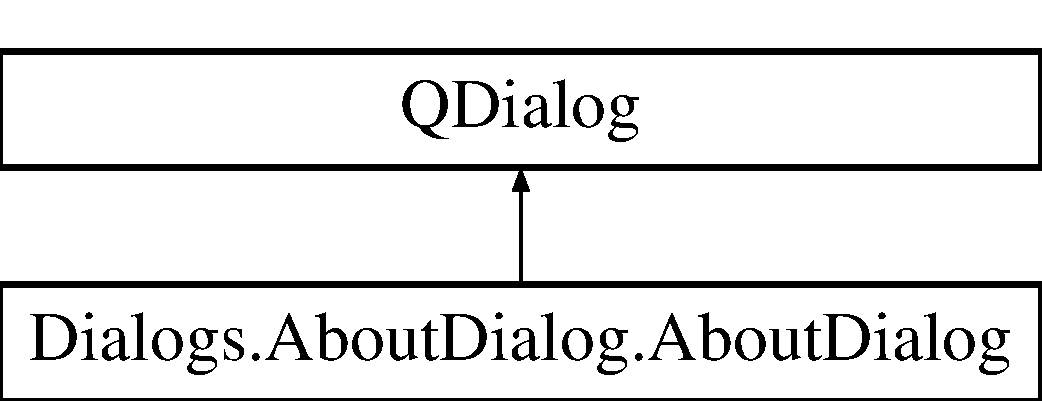
\includegraphics[height=2.000000cm]{classDialogs_1_1AboutDialog_1_1AboutDialog}
\end{center}
\end{figure}
\subsection*{Public Member Functions}
\begin{DoxyCompactItemize}
\item 
def \hyperlink{classDialogs_1_1AboutDialog_1_1AboutDialog_a403ad7b77ba4a388a5115edbe2dc1b5e}{\-\_\-\-\_\-init\-\_\-\-\_\-}
\item 
def \hyperlink{classDialogs_1_1AboutDialog_1_1AboutDialog_a8dfef3081ffaf5e468b66648f6bcbfce}{close\-Event}
\end{DoxyCompactItemize}
\subsection*{Public Attributes}
\begin{DoxyCompactItemize}
\item 
\hypertarget{classDialogs_1_1AboutDialog_1_1AboutDialog_ace06b14a19aa92cb6cf0095c6e26ea25}{{\bfseries ui}}\label{classDialogs_1_1AboutDialog_1_1AboutDialog_ace06b14a19aa92cb6cf0095c6e26ea25}

\item 
\hypertarget{classDialogs_1_1AboutDialog_1_1AboutDialog_afdbd3594cf0ef9704e60d657a22db4ff}{{\bfseries x}}\label{classDialogs_1_1AboutDialog_1_1AboutDialog_afdbd3594cf0ef9704e60d657a22db4ff}

\item 
\hypertarget{classDialogs_1_1AboutDialog_1_1AboutDialog_af58d38e97765d2398cc2f7337864cee8}{{\bfseries y}}\label{classDialogs_1_1AboutDialog_1_1AboutDialog_af58d38e97765d2398cc2f7337864cee8}

\item 
\hypertarget{classDialogs_1_1AboutDialog_1_1AboutDialog_a1185381f4c28ec38fc3457b078a4739e}{{\bfseries z}}\label{classDialogs_1_1AboutDialog_1_1AboutDialog_a1185381f4c28ec38fc3457b078a4739e}

\item 
\hypertarget{classDialogs_1_1AboutDialog_1_1AboutDialog_a935e7f3ac0a659f1ce7a51ac4ad607b9}{{\bfseries color\-\_\-\-R}}\label{classDialogs_1_1AboutDialog_1_1AboutDialog_a935e7f3ac0a659f1ce7a51ac4ad607b9}

\item 
\hypertarget{classDialogs_1_1AboutDialog_1_1AboutDialog_a374f448efb72ae5c4f8c75a78bfb8424}{{\bfseries color\-\_\-\-G}}\label{classDialogs_1_1AboutDialog_1_1AboutDialog_a374f448efb72ae5c4f8c75a78bfb8424}

\item 
\hypertarget{classDialogs_1_1AboutDialog_1_1AboutDialog_a2b09bdcfe10fa2234e995ebb340c93b8}{{\bfseries color\-\_\-\-B}}\label{classDialogs_1_1AboutDialog_1_1AboutDialog_a2b09bdcfe10fa2234e995ebb340c93b8}

\end{DoxyCompactItemize}


\subsection{Detailed Description}
\begin{DoxyVerb}About dialog that shows information about the program itself.
\end{DoxyVerb}
 

\subsection{Constructor \& Destructor Documentation}
\hypertarget{classDialogs_1_1AboutDialog_1_1AboutDialog_a403ad7b77ba4a388a5115edbe2dc1b5e}{\index{Dialogs\-::\-About\-Dialog\-::\-About\-Dialog@{Dialogs\-::\-About\-Dialog\-::\-About\-Dialog}!\-\_\-\-\_\-init\-\_\-\-\_\-@{\-\_\-\-\_\-init\-\_\-\-\_\-}}
\index{\-\_\-\-\_\-init\-\_\-\-\_\-@{\-\_\-\-\_\-init\-\_\-\-\_\-}!Dialogs::AboutDialog::AboutDialog@{Dialogs\-::\-About\-Dialog\-::\-About\-Dialog}}
\subsubsection[{\-\_\-\-\_\-init\-\_\-\-\_\-}]{\setlength{\rightskip}{0pt plus 5cm}def Dialogs.\-About\-Dialog.\-About\-Dialog.\-\_\-\-\_\-init\-\_\-\-\_\- (
\begin{DoxyParamCaption}
\item[{}]{self}
\end{DoxyParamCaption}
)}}\label{classDialogs_1_1AboutDialog_1_1AboutDialog_a403ad7b77ba4a388a5115edbe2dc1b5e}
\begin{DoxyVerb}Inits the About Dialog.
\end{DoxyVerb}
 

\subsection{Member Function Documentation}
\hypertarget{classDialogs_1_1AboutDialog_1_1AboutDialog_a8dfef3081ffaf5e468b66648f6bcbfce}{\index{Dialogs\-::\-About\-Dialog\-::\-About\-Dialog@{Dialogs\-::\-About\-Dialog\-::\-About\-Dialog}!close\-Event@{close\-Event}}
\index{close\-Event@{close\-Event}!Dialogs::AboutDialog::AboutDialog@{Dialogs\-::\-About\-Dialog\-::\-About\-Dialog}}
\subsubsection[{close\-Event}]{\setlength{\rightskip}{0pt plus 5cm}def Dialogs.\-About\-Dialog.\-About\-Dialog.\-close\-Event (
\begin{DoxyParamCaption}
\item[{}]{self, }
\item[{}]{event}
\end{DoxyParamCaption}
)}}\label{classDialogs_1_1AboutDialog_1_1AboutDialog_a8dfef3081ffaf5e468b66648f6bcbfce}
\begin{DoxyVerb}Proper closing.
\end{DoxyVerb}
 

The documentation for this class was generated from the following file\-:\begin{DoxyCompactItemize}
\item 
Dialogs/About\-Dialog.\-py\end{DoxyCompactItemize}

\hypertarget{classModules_1_1Selection_1_1AxesLimits}{\section{Modules.\-Selection.\-Axes\-Limits Class Reference}
\label{classModules_1_1Selection_1_1AxesLimits}\index{Modules.\-Selection.\-Axes\-Limits@{Modules.\-Selection.\-Axes\-Limits}}
}
\subsection*{Public Member Functions}
\begin{DoxyCompactItemize}
\item 
def \hyperlink{classModules_1_1Selection_1_1AxesLimits_a8aa4aee843f01541dc6e87be1e408074}{\-\_\-\-\_\-init\-\_\-\-\_\-}
\item 
def \hyperlink{classModules_1_1Selection_1_1AxesLimits_a17e9d42a2ee849582e6a0d4d7f79b817}{update\-\_\-limits}
\item 
def \hyperlink{classModules_1_1Selection_1_1AxesLimits_a0b096cac2c88b8f673649bd8177e21e9}{is\-\_\-inside}
\end{DoxyCompactItemize}


\subsection{Constructor \& Destructor Documentation}
\hypertarget{classModules_1_1Selection_1_1AxesLimits_a8aa4aee843f01541dc6e87be1e408074}{\index{Modules\-::\-Selection\-::\-Axes\-Limits@{Modules\-::\-Selection\-::\-Axes\-Limits}!\-\_\-\-\_\-init\-\_\-\-\_\-@{\-\_\-\-\_\-init\-\_\-\-\_\-}}
\index{\-\_\-\-\_\-init\-\_\-\-\_\-@{\-\_\-\-\_\-init\-\_\-\-\_\-}!Modules::Selection::AxesLimits@{Modules\-::\-Selection\-::\-Axes\-Limits}}
\subsubsection[{\-\_\-\-\_\-init\-\_\-\-\_\-}]{\setlength{\rightskip}{0pt plus 5cm}def Modules.\-Selection.\-Axes\-Limits.\-\_\-\-\_\-init\-\_\-\-\_\- (
\begin{DoxyParamCaption}
\item[{}]{self}
\end{DoxyParamCaption}
)}}\label{classModules_1_1Selection_1_1AxesLimits_a8aa4aee843f01541dc6e87be1e408074}
\begin{DoxyVerb}Inits axes limits
\end{DoxyVerb}
 

\subsection{Member Function Documentation}
\hypertarget{classModules_1_1Selection_1_1AxesLimits_a0b096cac2c88b8f673649bd8177e21e9}{\index{Modules\-::\-Selection\-::\-Axes\-Limits@{Modules\-::\-Selection\-::\-Axes\-Limits}!is\-\_\-inside@{is\-\_\-inside}}
\index{is\-\_\-inside@{is\-\_\-inside}!Modules::Selection::AxesLimits@{Modules\-::\-Selection\-::\-Axes\-Limits}}
\subsubsection[{is\-\_\-inside}]{\setlength{\rightskip}{0pt plus 5cm}def Modules.\-Selection.\-Axes\-Limits.\-is\-\_\-inside (
\begin{DoxyParamCaption}
\item[{}]{self, }
\item[{}]{point}
\end{DoxyParamCaption}
)}}\label{classModules_1_1Selection_1_1AxesLimits_a0b096cac2c88b8f673649bd8177e21e9}
\begin{DoxyVerb}Is point inside limits.

Args:
    point: A point as list (x, y) representing point.
    
Return:
    Returns True when point is within limits.
\end{DoxyVerb}
 \hypertarget{classModules_1_1Selection_1_1AxesLimits_a17e9d42a2ee849582e6a0d4d7f79b817}{\index{Modules\-::\-Selection\-::\-Axes\-Limits@{Modules\-::\-Selection\-::\-Axes\-Limits}!update\-\_\-limits@{update\-\_\-limits}}
\index{update\-\_\-limits@{update\-\_\-limits}!Modules::Selection::AxesLimits@{Modules\-::\-Selection\-::\-Axes\-Limits}}
\subsubsection[{update\-\_\-limits}]{\setlength{\rightskip}{0pt plus 5cm}def Modules.\-Selection.\-Axes\-Limits.\-update\-\_\-limits (
\begin{DoxyParamCaption}
\item[{}]{self, }
\item[{}]{point}
\end{DoxyParamCaption}
)}}\label{classModules_1_1Selection_1_1AxesLimits_a17e9d42a2ee849582e6a0d4d7f79b817}
\begin{DoxyVerb}Updates axes limits.

Args:
    point: A point as list (x, y) representing point.
\end{DoxyVerb}
 

The documentation for this class was generated from the following file\-:\begin{DoxyCompactItemize}
\item 
Modules/Selection.\-py\end{DoxyCompactItemize}

\hypertarget{classDialogs_1_1CalibrationDialog_1_1CalibrationCurveFittingWidget}{\section{Dialogs.\-Calibration\-Dialog.\-Calibration\-Curve\-Fitting\-Widget Class Reference}
\label{classDialogs_1_1CalibrationDialog_1_1CalibrationCurveFittingWidget}\index{Dialogs.\-Calibration\-Dialog.\-Calibration\-Curve\-Fitting\-Widget@{Dialogs.\-Calibration\-Dialog.\-Calibration\-Curve\-Fitting\-Widget}}
}
Inheritance diagram for Dialogs.\-Calibration\-Dialog.\-Calibration\-Curve\-Fitting\-Widget\-:\begin{figure}[H]
\begin{center}
\leavevmode
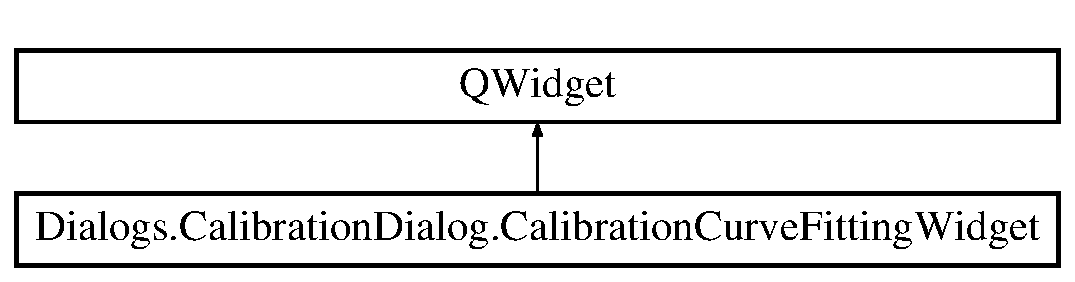
\includegraphics[height=2.000000cm]{classDialogs_1_1CalibrationDialog_1_1CalibrationCurveFittingWidget}
\end{center}
\end{figure}
\subsection*{Public Member Functions}
\begin{DoxyCompactItemize}
\item 
def \hyperlink{classDialogs_1_1CalibrationDialog_1_1CalibrationCurveFittingWidget_a35b7481066c5991eca76355975dcee85}{\-\_\-\-\_\-init\-\_\-\-\_\-}
\end{DoxyCompactItemize}
\subsection*{Public Attributes}
\begin{DoxyCompactItemize}
\item 
\hypertarget{classDialogs_1_1CalibrationDialog_1_1CalibrationCurveFittingWidget_a5ed7176f8414595efff19c74a552d5e0}{{\bfseries ui}}\label{classDialogs_1_1CalibrationDialog_1_1CalibrationCurveFittingWidget_a5ed7176f8414595efff19c74a552d5e0}

\item 
\hypertarget{classDialogs_1_1CalibrationDialog_1_1CalibrationCurveFittingWidget_a959f959cf28e9c23e84df700326bf516}{{\bfseries img\-\_\-dir}}\label{classDialogs_1_1CalibrationDialog_1_1CalibrationCurveFittingWidget_a959f959cf28e9c23e84df700326bf516}

\item 
\hypertarget{classDialogs_1_1CalibrationDialog_1_1CalibrationCurveFittingWidget_ab03709c7667d4a969e9d2cb16f724e33}{{\bfseries matplotlib}}\label{classDialogs_1_1CalibrationDialog_1_1CalibrationCurveFittingWidget_ab03709c7667d4a969e9d2cb16f724e33}

\end{DoxyCompactItemize}


\subsection{Detailed Description}
\begin{DoxyVerb}Widget class for holding MatplotlibCalibrationCurveFittingWidget.
\end{DoxyVerb}
 

\subsection{Constructor \& Destructor Documentation}
\hypertarget{classDialogs_1_1CalibrationDialog_1_1CalibrationCurveFittingWidget_a35b7481066c5991eca76355975dcee85}{\index{Dialogs\-::\-Calibration\-Dialog\-::\-Calibration\-Curve\-Fitting\-Widget@{Dialogs\-::\-Calibration\-Dialog\-::\-Calibration\-Curve\-Fitting\-Widget}!\-\_\-\-\_\-init\-\_\-\-\_\-@{\-\_\-\-\_\-init\-\_\-\-\_\-}}
\index{\-\_\-\-\_\-init\-\_\-\-\_\-@{\-\_\-\-\_\-init\-\_\-\-\_\-}!Dialogs::CalibrationDialog::CalibrationCurveFittingWidget@{Dialogs\-::\-Calibration\-Dialog\-::\-Calibration\-Curve\-Fitting\-Widget}}
\subsubsection[{\-\_\-\-\_\-init\-\_\-\-\_\-}]{\setlength{\rightskip}{0pt plus 5cm}def Dialogs.\-Calibration\-Dialog.\-Calibration\-Curve\-Fitting\-Widget.\-\_\-\-\_\-init\-\_\-\-\_\- (
\begin{DoxyParamCaption}
\item[{}]{self, }
\item[{}]{dialog, }
\item[{}]{cut, }
\item[{}]{tof\-\_\-calibration, }
\item[{}]{settings, }
\item[{}]{bin\-\_\-width, }
\item[{}]{column, }
\item[{}]{masses}
\end{DoxyParamCaption}
)}}\label{classDialogs_1_1CalibrationDialog_1_1CalibrationCurveFittingWidget_a35b7481066c5991eca76355975dcee85}
\begin{DoxyVerb}Inits widget.

Args:
    dialog: Parent dialog.
    cut: CutFile class object.
    tof_calibration: TOFCalibration class object.
    settings: Settings object
    bin_width: Float representing histogram's bin width.
    column: Integer representing which column number is used.
    masses: Reference to Masses class object.
\end{DoxyVerb}
 

The documentation for this class was generated from the following file\-:\begin{DoxyCompactItemize}
\item 
Dialogs/Calibration\-Dialog.\-py\end{DoxyCompactItemize}

\hypertarget{classDialogs_1_1CalibrationDialog_1_1CalibrationDialog}{\section{Dialogs.\-Calibration\-Dialog.\-Calibration\-Dialog Class Reference}
\label{classDialogs_1_1CalibrationDialog_1_1CalibrationDialog}\index{Dialogs.\-Calibration\-Dialog.\-Calibration\-Dialog@{Dialogs.\-Calibration\-Dialog.\-Calibration\-Dialog}}
}
Inheritance diagram for Dialogs.\-Calibration\-Dialog.\-Calibration\-Dialog\-:\begin{figure}[H]
\begin{center}
\leavevmode
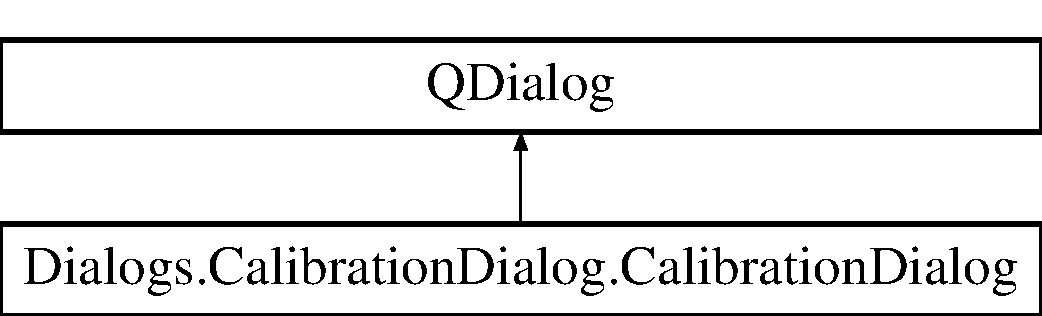
\includegraphics[height=2.000000cm]{classDialogs_1_1CalibrationDialog_1_1CalibrationDialog}
\end{center}
\end{figure}
\subsection*{Public Member Functions}
\begin{DoxyCompactItemize}
\item 
def \hyperlink{classDialogs_1_1CalibrationDialog_1_1CalibrationDialog_a187759c1babdaa11a4f6bc9988c83d30}{\-\_\-\-\_\-init\-\_\-\-\_\-}
\item 
def \hyperlink{classDialogs_1_1CalibrationDialog_1_1CalibrationDialog_a2bc841733761278b2d3db45e9d1f98de}{remove\-\_\-selected\-\_\-points}
\item 
def \hyperlink{classDialogs_1_1CalibrationDialog_1_1CalibrationDialog_a3391e2bc6c7a8b8f65b86f32f3b2794b}{set\-\_\-calibration\-\_\-point}
\item 
def \hyperlink{classDialogs_1_1CalibrationDialog_1_1CalibrationDialog_a93c6577ff5f78c87c49519aebd6b48d9}{set\-\_\-calibration\-\_\-parameters\-\_\-to\-\_\-parent}
\item 
def \hyperlink{classDialogs_1_1CalibrationDialog_1_1CalibrationDialog_a8d446c99157afc3c8871d155c55a26c9}{accept\-\_\-calibration}
\item 
def \hyperlink{classDialogs_1_1CalibrationDialog_1_1CalibrationDialog_a62fe769b56ecb7dec14b6e14542e461c}{change\-\_\-current\-\_\-cut}
\item 
def \hyperlink{classDialogs_1_1CalibrationDialog_1_1CalibrationDialog_a16592d0bc33cb3e74caf02be88d24441}{timeout}
\end{DoxyCompactItemize}
\subsection*{Public Attributes}
\begin{DoxyCompactItemize}
\item 
\hypertarget{classDialogs_1_1CalibrationDialog_1_1CalibrationDialog_a776b0f68b7065a8504c279b756efb1b6}{{\bfseries measurements}}\label{classDialogs_1_1CalibrationDialog_1_1CalibrationDialog_a776b0f68b7065a8504c279b756efb1b6}

\item 
\hypertarget{classDialogs_1_1CalibrationDialog_1_1CalibrationDialog_a7dec9b9ce3f146cda1d5e56b6aaa6f5f}{{\bfseries settings}}\label{classDialogs_1_1CalibrationDialog_1_1CalibrationDialog_a7dec9b9ce3f146cda1d5e56b6aaa6f5f}

\item 
\hypertarget{classDialogs_1_1CalibrationDialog_1_1CalibrationDialog_a31c95bf50bcf3af0942721d2d4e95abd}{{\bfseries ui}}\label{classDialogs_1_1CalibrationDialog_1_1CalibrationDialog_a31c95bf50bcf3af0942721d2d4e95abd}

\item 
\hypertarget{classDialogs_1_1CalibrationDialog_1_1CalibrationDialog_a597d5f72532849167f1a34c459d944ae}{{\bfseries parent\-\_\-settings\-\_\-dialog}}\label{classDialogs_1_1CalibrationDialog_1_1CalibrationDialog_a597d5f72532849167f1a34c459d944ae}

\item 
\hypertarget{classDialogs_1_1CalibrationDialog_1_1CalibrationDialog_af5e6800ae159337609f6a4fd7699fb74}{{\bfseries tof\-\_\-calibration}}\label{classDialogs_1_1CalibrationDialog_1_1CalibrationDialog_af5e6800ae159337609f6a4fd7699fb74}

\item 
\hypertarget{classDialogs_1_1CalibrationDialog_1_1CalibrationDialog_a2e57be58624098dc3e01aa6aaf33fd48}{{\bfseries curve\-Fitting\-Widget}}\label{classDialogs_1_1CalibrationDialog_1_1CalibrationDialog_a2e57be58624098dc3e01aa6aaf33fd48}

\item 
\hypertarget{classDialogs_1_1CalibrationDialog_1_1CalibrationDialog_ae9afb1da1d9254018281b8beea206e83}{{\bfseries linear\-Fitting\-Widget}}\label{classDialogs_1_1CalibrationDialog_1_1CalibrationDialog_ae9afb1da1d9254018281b8beea206e83}

\item 
\hypertarget{classDialogs_1_1CalibrationDialog_1_1CalibrationDialog_a2c6ceb6e312a97e66b810957135829e3}{{\bfseries timer}}\label{classDialogs_1_1CalibrationDialog_1_1CalibrationDialog_a2c6ceb6e312a97e66b810957135829e3}

\end{DoxyCompactItemize}


\subsection{Detailed Description}
\begin{DoxyVerb}A dialog for the time of flight calibration
\end{DoxyVerb}
 

\subsection{Constructor \& Destructor Documentation}
\hypertarget{classDialogs_1_1CalibrationDialog_1_1CalibrationDialog_a187759c1babdaa11a4f6bc9988c83d30}{\index{Dialogs\-::\-Calibration\-Dialog\-::\-Calibration\-Dialog@{Dialogs\-::\-Calibration\-Dialog\-::\-Calibration\-Dialog}!\-\_\-\-\_\-init\-\_\-\-\_\-@{\-\_\-\-\_\-init\-\_\-\-\_\-}}
\index{\-\_\-\-\_\-init\-\_\-\-\_\-@{\-\_\-\-\_\-init\-\_\-\-\_\-}!Dialogs::CalibrationDialog::CalibrationDialog@{Dialogs\-::\-Calibration\-Dialog\-::\-Calibration\-Dialog}}
\subsubsection[{\-\_\-\-\_\-init\-\_\-\-\_\-}]{\setlength{\rightskip}{0pt plus 5cm}def Dialogs.\-Calibration\-Dialog.\-Calibration\-Dialog.\-\_\-\-\_\-init\-\_\-\-\_\- (
\begin{DoxyParamCaption}
\item[{}]{self, }
\item[{}]{measurements, }
\item[{}]{settings, }
\item[{}]{masses, }
\item[{}]{parent\-\_\-settings\-\_\-dialog = {\ttfamily None}}
\end{DoxyParamCaption}
)}}\label{classDialogs_1_1CalibrationDialog_1_1CalibrationDialog_a187759c1babdaa11a4f6bc9988c83d30}
\begin{DoxyVerb}Inits the calibration dialog class.

Args:
    measurements: A string list representing measurements files.
    settings: A Settings class object.
    masses: A Masses class object.
    parent_settings_dialog: A representing from which dialog this was 
                    opened from.
\end{DoxyVerb}
 

\subsection{Member Function Documentation}
\hypertarget{classDialogs_1_1CalibrationDialog_1_1CalibrationDialog_a8d446c99157afc3c8871d155c55a26c9}{\index{Dialogs\-::\-Calibration\-Dialog\-::\-Calibration\-Dialog@{Dialogs\-::\-Calibration\-Dialog\-::\-Calibration\-Dialog}!accept\-\_\-calibration@{accept\-\_\-calibration}}
\index{accept\-\_\-calibration@{accept\-\_\-calibration}!Dialogs::CalibrationDialog::CalibrationDialog@{Dialogs\-::\-Calibration\-Dialog\-::\-Calibration\-Dialog}}
\subsubsection[{accept\-\_\-calibration}]{\setlength{\rightskip}{0pt plus 5cm}def Dialogs.\-Calibration\-Dialog.\-Calibration\-Dialog.\-accept\-\_\-calibration (
\begin{DoxyParamCaption}
\item[{}]{self}
\end{DoxyParamCaption}
)}}\label{classDialogs_1_1CalibrationDialog_1_1CalibrationDialog_a8d446c99157afc3c8871d155c55a26c9}
\begin{DoxyVerb}Accept calibration (parameters).
\end{DoxyVerb}
 \hypertarget{classDialogs_1_1CalibrationDialog_1_1CalibrationDialog_a62fe769b56ecb7dec14b6e14542e461c}{\index{Dialogs\-::\-Calibration\-Dialog\-::\-Calibration\-Dialog@{Dialogs\-::\-Calibration\-Dialog\-::\-Calibration\-Dialog}!change\-\_\-current\-\_\-cut@{change\-\_\-current\-\_\-cut}}
\index{change\-\_\-current\-\_\-cut@{change\-\_\-current\-\_\-cut}!Dialogs::CalibrationDialog::CalibrationDialog@{Dialogs\-::\-Calibration\-Dialog\-::\-Calibration\-Dialog}}
\subsubsection[{change\-\_\-current\-\_\-cut}]{\setlength{\rightskip}{0pt plus 5cm}def Dialogs.\-Calibration\-Dialog.\-Calibration\-Dialog.\-change\-\_\-current\-\_\-cut (
\begin{DoxyParamCaption}
\item[{}]{self, }
\item[{}]{current\-\_\-item}
\end{DoxyParamCaption}
)}}\label{classDialogs_1_1CalibrationDialog_1_1CalibrationDialog_a62fe769b56ecb7dec14b6e14542e461c}
\begin{DoxyVerb}Changes the current cut file drawn to the curve fitting widget.

Args:
    current_item: QtWidgets.QTreeWidgetItem of CutFile which was selected.
\end{DoxyVerb}
 \hypertarget{classDialogs_1_1CalibrationDialog_1_1CalibrationDialog_a2bc841733761278b2d3db45e9d1f98de}{\index{Dialogs\-::\-Calibration\-Dialog\-::\-Calibration\-Dialog@{Dialogs\-::\-Calibration\-Dialog\-::\-Calibration\-Dialog}!remove\-\_\-selected\-\_\-points@{remove\-\_\-selected\-\_\-points}}
\index{remove\-\_\-selected\-\_\-points@{remove\-\_\-selected\-\_\-points}!Dialogs::CalibrationDialog::CalibrationDialog@{Dialogs\-::\-Calibration\-Dialog\-::\-Calibration\-Dialog}}
\subsubsection[{remove\-\_\-selected\-\_\-points}]{\setlength{\rightskip}{0pt plus 5cm}def Dialogs.\-Calibration\-Dialog.\-Calibration\-Dialog.\-remove\-\_\-selected\-\_\-points (
\begin{DoxyParamCaption}
\item[{}]{self}
\end{DoxyParamCaption}
)}}\label{classDialogs_1_1CalibrationDialog_1_1CalibrationDialog_a2bc841733761278b2d3db45e9d1f98de}
\begin{DoxyVerb}Remove selected items from point tree widget
\end{DoxyVerb}
 \hypertarget{classDialogs_1_1CalibrationDialog_1_1CalibrationDialog_a93c6577ff5f78c87c49519aebd6b48d9}{\index{Dialogs\-::\-Calibration\-Dialog\-::\-Calibration\-Dialog@{Dialogs\-::\-Calibration\-Dialog\-::\-Calibration\-Dialog}!set\-\_\-calibration\-\_\-parameters\-\_\-to\-\_\-parent@{set\-\_\-calibration\-\_\-parameters\-\_\-to\-\_\-parent}}
\index{set\-\_\-calibration\-\_\-parameters\-\_\-to\-\_\-parent@{set\-\_\-calibration\-\_\-parameters\-\_\-to\-\_\-parent}!Dialogs::CalibrationDialog::CalibrationDialog@{Dialogs\-::\-Calibration\-Dialog\-::\-Calibration\-Dialog}}
\subsubsection[{set\-\_\-calibration\-\_\-parameters\-\_\-to\-\_\-parent}]{\setlength{\rightskip}{0pt plus 5cm}def Dialogs.\-Calibration\-Dialog.\-Calibration\-Dialog.\-set\-\_\-calibration\-\_\-parameters\-\_\-to\-\_\-parent (
\begin{DoxyParamCaption}
\item[{}]{self}
\end{DoxyParamCaption}
)}}\label{classDialogs_1_1CalibrationDialog_1_1CalibrationDialog_a93c6577ff5f78c87c49519aebd6b48d9}
\begin{DoxyVerb}Set calibration parameters to parent dialog's calibration parameters 
fields.
\end{DoxyVerb}
 \hypertarget{classDialogs_1_1CalibrationDialog_1_1CalibrationDialog_a3391e2bc6c7a8b8f65b86f32f3b2794b}{\index{Dialogs\-::\-Calibration\-Dialog\-::\-Calibration\-Dialog@{Dialogs\-::\-Calibration\-Dialog\-::\-Calibration\-Dialog}!set\-\_\-calibration\-\_\-point@{set\-\_\-calibration\-\_\-point}}
\index{set\-\_\-calibration\-\_\-point@{set\-\_\-calibration\-\_\-point}!Dialogs::CalibrationDialog::CalibrationDialog@{Dialogs\-::\-Calibration\-Dialog\-::\-Calibration\-Dialog}}
\subsubsection[{set\-\_\-calibration\-\_\-point}]{\setlength{\rightskip}{0pt plus 5cm}def Dialogs.\-Calibration\-Dialog.\-Calibration\-Dialog.\-set\-\_\-calibration\-\_\-point (
\begin{DoxyParamCaption}
\item[{}]{self, }
\item[{}]{tof}
\end{DoxyParamCaption}
)}}\label{classDialogs_1_1CalibrationDialog_1_1CalibrationDialog_a3391e2bc6c7a8b8f65b86f32f3b2794b}
\begin{DoxyVerb}Set Cut file front edge estimation to specific value.

Args:
    tof: Float representing front edge of linear fit estimation.
\end{DoxyVerb}
 \hypertarget{classDialogs_1_1CalibrationDialog_1_1CalibrationDialog_a16592d0bc33cb3e74caf02be88d24441}{\index{Dialogs\-::\-Calibration\-Dialog\-::\-Calibration\-Dialog@{Dialogs\-::\-Calibration\-Dialog\-::\-Calibration\-Dialog}!timeout@{timeout}}
\index{timeout@{timeout}!Dialogs::CalibrationDialog::CalibrationDialog@{Dialogs\-::\-Calibration\-Dialog\-::\-Calibration\-Dialog}}
\subsubsection[{timeout}]{\setlength{\rightskip}{0pt plus 5cm}def Dialogs.\-Calibration\-Dialog.\-Calibration\-Dialog.\-timeout (
\begin{DoxyParamCaption}
\item[{}]{self}
\end{DoxyParamCaption}
)}}\label{classDialogs_1_1CalibrationDialog_1_1CalibrationDialog_a16592d0bc33cb3e74caf02be88d24441}
\begin{DoxyVerb}Timeout eventmethod to remove label text.
\end{DoxyVerb}
 

The documentation for this class was generated from the following file\-:\begin{DoxyCompactItemize}
\item 
Dialogs/Calibration\-Dialog.\-py\end{DoxyCompactItemize}

\hypertarget{classDialogs_1_1CalibrationDialog_1_1CalibrationLinearFittingWidget}{\section{Dialogs.\-Calibration\-Dialog.\-Calibration\-Linear\-Fitting\-Widget Class Reference}
\label{classDialogs_1_1CalibrationDialog_1_1CalibrationLinearFittingWidget}\index{Dialogs.\-Calibration\-Dialog.\-Calibration\-Linear\-Fitting\-Widget@{Dialogs.\-Calibration\-Dialog.\-Calibration\-Linear\-Fitting\-Widget}}
}
Inheritance diagram for Dialogs.\-Calibration\-Dialog.\-Calibration\-Linear\-Fitting\-Widget\-:\begin{figure}[H]
\begin{center}
\leavevmode
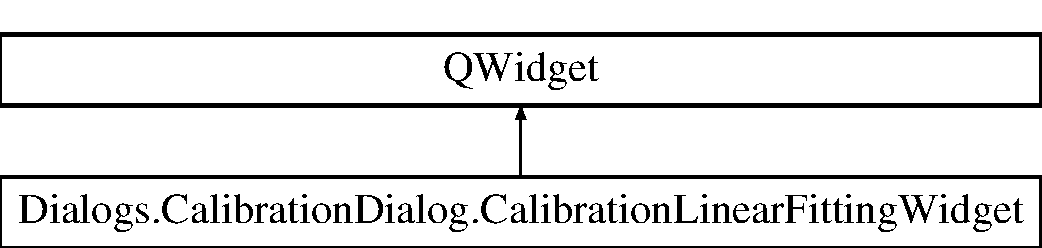
\includegraphics[height=2.000000cm]{classDialogs_1_1CalibrationDialog_1_1CalibrationLinearFittingWidget}
\end{center}
\end{figure}
\subsection*{Public Member Functions}
\begin{DoxyCompactItemize}
\item 
def \hyperlink{classDialogs_1_1CalibrationDialog_1_1CalibrationLinearFittingWidget_a0e2b28d1e603e4932aa85e4ca730247f}{\-\_\-\-\_\-init\-\_\-\-\_\-}
\end{DoxyCompactItemize}
\subsection*{Public Attributes}
\begin{DoxyCompactItemize}
\item 
\hypertarget{classDialogs_1_1CalibrationDialog_1_1CalibrationLinearFittingWidget_a914316b12db2f341067a6fe287159bb8}{{\bfseries ui}}\label{classDialogs_1_1CalibrationDialog_1_1CalibrationLinearFittingWidget_a914316b12db2f341067a6fe287159bb8}

\item 
\hypertarget{classDialogs_1_1CalibrationDialog_1_1CalibrationLinearFittingWidget_afc2b3b32f0770758bddf99e17289259e}{{\bfseries img\-\_\-dir}}\label{classDialogs_1_1CalibrationDialog_1_1CalibrationLinearFittingWidget_afc2b3b32f0770758bddf99e17289259e}

\item 
\hypertarget{classDialogs_1_1CalibrationDialog_1_1CalibrationLinearFittingWidget_a3eaebbfa5e145bc190141628ff7f6d63}{{\bfseries matplotlib}}\label{classDialogs_1_1CalibrationDialog_1_1CalibrationLinearFittingWidget_a3eaebbfa5e145bc190141628ff7f6d63}

\end{DoxyCompactItemize}


\subsection{Detailed Description}
\begin{DoxyVerb}Widget class for holding MatplotlibCalibrationLinearFittingWidget.
\end{DoxyVerb}
 

\subsection{Constructor \& Destructor Documentation}
\hypertarget{classDialogs_1_1CalibrationDialog_1_1CalibrationLinearFittingWidget_a0e2b28d1e603e4932aa85e4ca730247f}{\index{Dialogs\-::\-Calibration\-Dialog\-::\-Calibration\-Linear\-Fitting\-Widget@{Dialogs\-::\-Calibration\-Dialog\-::\-Calibration\-Linear\-Fitting\-Widget}!\-\_\-\-\_\-init\-\_\-\-\_\-@{\-\_\-\-\_\-init\-\_\-\-\_\-}}
\index{\-\_\-\-\_\-init\-\_\-\-\_\-@{\-\_\-\-\_\-init\-\_\-\-\_\-}!Dialogs::CalibrationDialog::CalibrationLinearFittingWidget@{Dialogs\-::\-Calibration\-Dialog\-::\-Calibration\-Linear\-Fitting\-Widget}}
\subsubsection[{\-\_\-\-\_\-init\-\_\-\-\_\-}]{\setlength{\rightskip}{0pt plus 5cm}def Dialogs.\-Calibration\-Dialog.\-Calibration\-Linear\-Fitting\-Widget.\-\_\-\-\_\-init\-\_\-\-\_\- (
\begin{DoxyParamCaption}
\item[{}]{self, }
\item[{}]{dialog, }
\item[{}]{tof\-\_\-calibration, }
\item[{}]{old\-\_\-params}
\end{DoxyParamCaption}
)}}\label{classDialogs_1_1CalibrationDialog_1_1CalibrationLinearFittingWidget_a0e2b28d1e603e4932aa85e4ca730247f}
\begin{DoxyVerb}Inits widget.

Args:
    dialog: Parent dialog.
    tof_calibration: TOFCalibration class object.
    old_params: Old calibration parameters in tuple (slope, offset).
\end{DoxyVerb}
 

The documentation for this class was generated from the following file\-:\begin{DoxyCompactItemize}
\item 
Dialogs/Calibration\-Dialog.\-py\end{DoxyCompactItemize}

\hypertarget{classModules_1_1CalibrationParameters_1_1CalibrationParameters}{\section{Modules.\-Calibration\-Parameters.\-Calibration\-Parameters Class Reference}
\label{classModules_1_1CalibrationParameters_1_1CalibrationParameters}\index{Modules.\-Calibration\-Parameters.\-Calibration\-Parameters@{Modules.\-Calibration\-Parameters.\-Calibration\-Parameters}}
}
\subsection*{Public Member Functions}
\begin{DoxyCompactItemize}
\item 
def \hyperlink{classModules_1_1CalibrationParameters_1_1CalibrationParameters_a95c95f05684d72250bddf7a46688e363}{\-\_\-\-\_\-init\-\_\-\-\_\-}
\item 
def \hyperlink{classModules_1_1CalibrationParameters_1_1CalibrationParameters_adb9ba4e01f0f198c0396c33cc2a74c8a}{show}
\item 
def \hyperlink{classModules_1_1CalibrationParameters_1_1CalibrationParameters_a40b7ae90349f9177ddaa1ebb576e8ac1}{set\-\_\-settings}
\item 
def \hyperlink{classModules_1_1CalibrationParameters_1_1CalibrationParameters_ac0a7bad8db5e7533f1d79c9b53718669}{load\-\_\-settings}
\item 
def \hyperlink{classModules_1_1CalibrationParameters_1_1CalibrationParameters_aaa58de4b3265a493e7572875e25bbf6e}{save\-\_\-settings}
\end{DoxyCompactItemize}
\subsection*{Public Attributes}
\begin{DoxyCompactItemize}
\item 
\hypertarget{classModules_1_1CalibrationParameters_1_1CalibrationParameters_aa467d1370c1ead3bdf99507f58cd49a0}{{\bfseries calibration\-\_\-settings\-\_\-filename}}\label{classModules_1_1CalibrationParameters_1_1CalibrationParameters_aa467d1370c1ead3bdf99507f58cd49a0}

\item 
\hypertarget{classModules_1_1CalibrationParameters_1_1CalibrationParameters_a430248744451617113e9b75f53bd9521}{{\bfseries config}}\label{classModules_1_1CalibrationParameters_1_1CalibrationParameters_a430248744451617113e9b75f53bd9521}

\item 
\hypertarget{classModules_1_1CalibrationParameters_1_1CalibrationParameters_a0a2abd1a55d3b70d0e671ecef7e8836e}{{\bfseries use\-\_\-settings}}\label{classModules_1_1CalibrationParameters_1_1CalibrationParameters_a0a2abd1a55d3b70d0e671ecef7e8836e}

\item 
\hypertarget{classModules_1_1CalibrationParameters_1_1CalibrationParameters_abb9fc2a4be1d18cdaa7a81b04d8f6c9b}{{\bfseries slope}}\label{classModules_1_1CalibrationParameters_1_1CalibrationParameters_abb9fc2a4be1d18cdaa7a81b04d8f6c9b}

\item 
\hypertarget{classModules_1_1CalibrationParameters_1_1CalibrationParameters_a6eed88f1ad9666e95401a93c53141f21}{{\bfseries offset}}\label{classModules_1_1CalibrationParameters_1_1CalibrationParameters_a6eed88f1ad9666e95401a93c53141f21}

\item 
\hypertarget{classModules_1_1CalibrationParameters_1_1CalibrationParameters_a3aeafae902db9870be121f324b647d14}{{\bfseries angleslope}}\label{classModules_1_1CalibrationParameters_1_1CalibrationParameters_a3aeafae902db9870be121f324b647d14}

\item 
\hypertarget{classModules_1_1CalibrationParameters_1_1CalibrationParameters_a90c0597110dd9f8c076d55934eedbbcc}{{\bfseries angleoffset}}\label{classModules_1_1CalibrationParameters_1_1CalibrationParameters_a90c0597110dd9f8c076d55934eedbbcc}

\item 
\hypertarget{classModules_1_1CalibrationParameters_1_1CalibrationParameters_aad3e7cf5d81fbc6be925f2d050cee03a}{{\bfseries filepath}}\label{classModules_1_1CalibrationParameters_1_1CalibrationParameters_aad3e7cf5d81fbc6be925f2d050cee03a}

\end{DoxyCompactItemize}


\subsection{Detailed Description}
\begin{DoxyVerb}MeasuringSettings holds the all project specific measurement unit parameters.
\end{DoxyVerb}
 

\subsection{Constructor \& Destructor Documentation}
\hypertarget{classModules_1_1CalibrationParameters_1_1CalibrationParameters_a95c95f05684d72250bddf7a46688e363}{\index{Modules\-::\-Calibration\-Parameters\-::\-Calibration\-Parameters@{Modules\-::\-Calibration\-Parameters\-::\-Calibration\-Parameters}!\-\_\-\-\_\-init\-\_\-\-\_\-@{\-\_\-\-\_\-init\-\_\-\-\_\-}}
\index{\-\_\-\-\_\-init\-\_\-\-\_\-@{\-\_\-\-\_\-init\-\_\-\-\_\-}!Modules::CalibrationParameters::CalibrationParameters@{Modules\-::\-Calibration\-Parameters\-::\-Calibration\-Parameters}}
\subsubsection[{\-\_\-\-\_\-init\-\_\-\-\_\-}]{\setlength{\rightskip}{0pt plus 5cm}def Modules.\-Calibration\-Parameters.\-Calibration\-Parameters.\-\_\-\-\_\-init\-\_\-\-\_\- (
\begin{DoxyParamCaption}
\item[{}]{self, }
\item[{}]{settings\-\_\-filepath = {\ttfamily None}}
\end{DoxyParamCaption}
)}}\label{classModules_1_1CalibrationParameters_1_1CalibrationParameters_a95c95f05684d72250bddf7a46688e363}
\begin{DoxyVerb}Inits MeasuringSettings.

Args:
    settings_filepath: filepath for the settings file to be loaded
\end{DoxyVerb}
 

\subsection{Member Function Documentation}
\hypertarget{classModules_1_1CalibrationParameters_1_1CalibrationParameters_ac0a7bad8db5e7533f1d79c9b53718669}{\index{Modules\-::\-Calibration\-Parameters\-::\-Calibration\-Parameters@{Modules\-::\-Calibration\-Parameters\-::\-Calibration\-Parameters}!load\-\_\-settings@{load\-\_\-settings}}
\index{load\-\_\-settings@{load\-\_\-settings}!Modules::CalibrationParameters::CalibrationParameters@{Modules\-::\-Calibration\-Parameters\-::\-Calibration\-Parameters}}
\subsubsection[{load\-\_\-settings}]{\setlength{\rightskip}{0pt plus 5cm}def Modules.\-Calibration\-Parameters.\-Calibration\-Parameters.\-load\-\_\-settings (
\begin{DoxyParamCaption}
\item[{}]{self, }
\item[{}]{filepath}
\end{DoxyParamCaption}
)}}\label{classModules_1_1CalibrationParameters_1_1CalibrationParameters_ac0a7bad8db5e7533f1d79c9b53718669}
\begin{DoxyVerb}Loads settings' parameters from the given filepath.

Args:
    filepath: Filepath to the settings file.
\end{DoxyVerb}
 \hypertarget{classModules_1_1CalibrationParameters_1_1CalibrationParameters_aaa58de4b3265a493e7572875e25bbf6e}{\index{Modules\-::\-Calibration\-Parameters\-::\-Calibration\-Parameters@{Modules\-::\-Calibration\-Parameters\-::\-Calibration\-Parameters}!save\-\_\-settings@{save\-\_\-settings}}
\index{save\-\_\-settings@{save\-\_\-settings}!Modules::CalibrationParameters::CalibrationParameters@{Modules\-::\-Calibration\-Parameters\-::\-Calibration\-Parameters}}
\subsubsection[{save\-\_\-settings}]{\setlength{\rightskip}{0pt plus 5cm}def Modules.\-Calibration\-Parameters.\-Calibration\-Parameters.\-save\-\_\-settings (
\begin{DoxyParamCaption}
\item[{}]{self, }
\item[{}]{filepath = {\ttfamily None}}
\end{DoxyParamCaption}
)}}\label{classModules_1_1CalibrationParameters_1_1CalibrationParameters_aaa58de4b3265a493e7572875e25bbf6e}
\begin{DoxyVerb}Saves settings' parameters to the given filepath.

Args:
    filepath: Filepath to the settings file.
\end{DoxyVerb}
 \hypertarget{classModules_1_1CalibrationParameters_1_1CalibrationParameters_a40b7ae90349f9177ddaa1ebb576e8ac1}{\index{Modules\-::\-Calibration\-Parameters\-::\-Calibration\-Parameters@{Modules\-::\-Calibration\-Parameters\-::\-Calibration\-Parameters}!set\-\_\-settings@{set\-\_\-settings}}
\index{set\-\_\-settings@{set\-\_\-settings}!Modules::CalibrationParameters::CalibrationParameters@{Modules\-::\-Calibration\-Parameters\-::\-Calibration\-Parameters}}
\subsubsection[{set\-\_\-settings}]{\setlength{\rightskip}{0pt plus 5cm}def Modules.\-Calibration\-Parameters.\-Calibration\-Parameters.\-set\-\_\-settings (
\begin{DoxyParamCaption}
\item[{}]{self, }
\item[{}]{dialog, }
\item[{}]{used\-\_\-settings = {\ttfamily None}}
\end{DoxyParamCaption}
)}}\label{classModules_1_1CalibrationParameters_1_1CalibrationParameters_a40b7ae90349f9177ddaa1ebb576e8ac1}
\begin{DoxyVerb}Takes inputted parameters from the given dialog and sets them to the 
corresponding object's parameters

Args:
    dialog: QDialog from which the parameters are taken.
\end{DoxyVerb}
 \hypertarget{classModules_1_1CalibrationParameters_1_1CalibrationParameters_adb9ba4e01f0f198c0396c33cc2a74c8a}{\index{Modules\-::\-Calibration\-Parameters\-::\-Calibration\-Parameters@{Modules\-::\-Calibration\-Parameters\-::\-Calibration\-Parameters}!show@{show}}
\index{show@{show}!Modules::CalibrationParameters::CalibrationParameters@{Modules\-::\-Calibration\-Parameters\-::\-Calibration\-Parameters}}
\subsubsection[{show}]{\setlength{\rightskip}{0pt plus 5cm}def Modules.\-Calibration\-Parameters.\-Calibration\-Parameters.\-show (
\begin{DoxyParamCaption}
\item[{}]{self, }
\item[{}]{dialog}
\end{DoxyParamCaption}
)}}\label{classModules_1_1CalibrationParameters_1_1CalibrationParameters_adb9ba4e01f0f198c0396c33cc2a74c8a}
\begin{DoxyVerb}Shows the measuring parameters in the given measuring settings dialog.

Args:
    dialog: QDialog whose fields are updated with the Calibration 
    parameters.
\end{DoxyVerb}
 

The documentation for this class was generated from the following file\-:\begin{DoxyCompactItemize}
\item 
Modules/Calibration\-Parameters.\-py\end{DoxyCompactItemize}

\hypertarget{classDialogs_1_1MeasurementSettingsDialogs_1_1CalibrationSettings}{\section{Dialogs.\-Measurement\-Settings\-Dialogs.\-Calibration\-Settings Class Reference}
\label{classDialogs_1_1MeasurementSettingsDialogs_1_1CalibrationSettings}\index{Dialogs.\-Measurement\-Settings\-Dialogs.\-Calibration\-Settings@{Dialogs.\-Measurement\-Settings\-Dialogs.\-Calibration\-Settings}}
}
Inheritance diagram for Dialogs.\-Measurement\-Settings\-Dialogs.\-Calibration\-Settings\-:\begin{figure}[H]
\begin{center}
\leavevmode
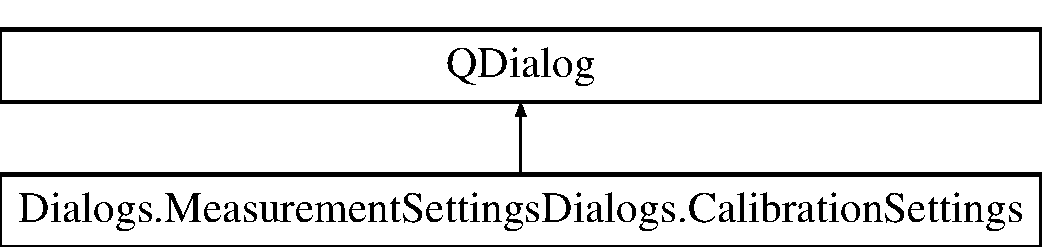
\includegraphics[height=2.000000cm]{classDialogs_1_1MeasurementSettingsDialogs_1_1CalibrationSettings}
\end{center}
\end{figure}
\subsection*{Public Member Functions}
\begin{DoxyCompactItemize}
\item 
def \hyperlink{classDialogs_1_1MeasurementSettingsDialogs_1_1CalibrationSettings_a8feb6db7e370d5493e59b6033455d0e1}{\-\_\-\-\_\-init\-\_\-\-\_\-}
\item 
def \hyperlink{classDialogs_1_1MeasurementSettingsDialogs_1_1CalibrationSettings_a97ca16f8cc439defb940360b5ce2298c}{update\-\_\-and\-\_\-close\-\_\-settings}
\end{DoxyCompactItemize}
\subsection*{Public Attributes}
\begin{DoxyCompactItemize}
\item 
\hypertarget{classDialogs_1_1MeasurementSettingsDialogs_1_1CalibrationSettings_a108762053de08985fcb24795bfb744f2}{{\bfseries default\-\_\-folder}}\label{classDialogs_1_1MeasurementSettingsDialogs_1_1CalibrationSettings_a108762053de08985fcb24795bfb744f2}

\item 
\hypertarget{classDialogs_1_1MeasurementSettingsDialogs_1_1CalibrationSettings_a7c9ac94edb76d01ec853b30eb9d4a13e}{{\bfseries measurement}}\label{classDialogs_1_1MeasurementSettingsDialogs_1_1CalibrationSettings_a7c9ac94edb76d01ec853b30eb9d4a13e}

\item 
\hypertarget{classDialogs_1_1MeasurementSettingsDialogs_1_1CalibrationSettings_a3a1867174c2200b1289f49ae14249be0}{{\bfseries masses}}\label{classDialogs_1_1MeasurementSettingsDialogs_1_1CalibrationSettings_a3a1867174c2200b1289f49ae14249be0}

\item 
\hypertarget{classDialogs_1_1MeasurementSettingsDialogs_1_1CalibrationSettings_a15807ee1ac0c9cf91b95645e1410cd00}{{\bfseries ui}}\label{classDialogs_1_1MeasurementSettingsDialogs_1_1CalibrationSettings_a15807ee1ac0c9cf91b95645e1410cd00}

\item 
\hypertarget{classDialogs_1_1MeasurementSettingsDialogs_1_1CalibrationSettings_af1a179a0fd488e9ba6c1bcfab5928860}{{\bfseries project\-\_\-settings}}\label{classDialogs_1_1MeasurementSettingsDialogs_1_1CalibrationSettings_af1a179a0fd488e9ba6c1bcfab5928860}

\item 
\hypertarget{classDialogs_1_1MeasurementSettingsDialogs_1_1CalibrationSettings_a9c7466ecbe2a9418d6a2721299102f38}{{\bfseries settings}}\label{classDialogs_1_1MeasurementSettingsDialogs_1_1CalibrationSettings_a9c7466ecbe2a9418d6a2721299102f38}

\end{DoxyCompactItemize}


\subsection{Constructor \& Destructor Documentation}
\hypertarget{classDialogs_1_1MeasurementSettingsDialogs_1_1CalibrationSettings_a8feb6db7e370d5493e59b6033455d0e1}{\index{Dialogs\-::\-Measurement\-Settings\-Dialogs\-::\-Calibration\-Settings@{Dialogs\-::\-Measurement\-Settings\-Dialogs\-::\-Calibration\-Settings}!\-\_\-\-\_\-init\-\_\-\-\_\-@{\-\_\-\-\_\-init\-\_\-\-\_\-}}
\index{\-\_\-\-\_\-init\-\_\-\-\_\-@{\-\_\-\-\_\-init\-\_\-\-\_\-}!Dialogs::MeasurementSettingsDialogs::CalibrationSettings@{Dialogs\-::\-Measurement\-Settings\-Dialogs\-::\-Calibration\-Settings}}
\subsubsection[{\-\_\-\-\_\-init\-\_\-\-\_\-}]{\setlength{\rightskip}{0pt plus 5cm}def Dialogs.\-Measurement\-Settings\-Dialogs.\-Calibration\-Settings.\-\_\-\-\_\-init\-\_\-\-\_\- (
\begin{DoxyParamCaption}
\item[{}]{self, }
\item[{}]{measurement}
\end{DoxyParamCaption}
)}}\label{classDialogs_1_1MeasurementSettingsDialogs_1_1CalibrationSettings_a8feb6db7e370d5493e59b6033455d0e1}
\begin{DoxyVerb}Constructor for the program

Args:
    measurement: Measurement class object.
\end{DoxyVerb}
 

\subsection{Member Function Documentation}
\hypertarget{classDialogs_1_1MeasurementSettingsDialogs_1_1CalibrationSettings_a97ca16f8cc439defb940360b5ce2298c}{\index{Dialogs\-::\-Measurement\-Settings\-Dialogs\-::\-Calibration\-Settings@{Dialogs\-::\-Measurement\-Settings\-Dialogs\-::\-Calibration\-Settings}!update\-\_\-and\-\_\-close\-\_\-settings@{update\-\_\-and\-\_\-close\-\_\-settings}}
\index{update\-\_\-and\-\_\-close\-\_\-settings@{update\-\_\-and\-\_\-close\-\_\-settings}!Dialogs::MeasurementSettingsDialogs::CalibrationSettings@{Dialogs\-::\-Measurement\-Settings\-Dialogs\-::\-Calibration\-Settings}}
\subsubsection[{update\-\_\-and\-\_\-close\-\_\-settings}]{\setlength{\rightskip}{0pt plus 5cm}def Dialogs.\-Measurement\-Settings\-Dialogs.\-Calibration\-Settings.\-update\-\_\-and\-\_\-close\-\_\-settings (
\begin{DoxyParamCaption}
\item[{}]{self}
\end{DoxyParamCaption}
)}}\label{classDialogs_1_1MeasurementSettingsDialogs_1_1CalibrationSettings_a97ca16f8cc439defb940360b5ce2298c}
\begin{DoxyVerb}Updates measuring settings values with the dialog's values and saves
them to default ini file.
\end{DoxyVerb}
 

The documentation for this class was generated from the following file\-:\begin{DoxyCompactItemize}
\item 
Dialogs/Measurement\-Settings\-Dialogs.\-py\end{DoxyCompactItemize}

\hypertarget{classDialogs_1_1ImportMeasurementDialog_1_1CoincTiming}{\section{Dialogs.\-Import\-Measurement\-Dialog.\-Coinc\-Timing Class Reference}
\label{classDialogs_1_1ImportMeasurementDialog_1_1CoincTiming}\index{Dialogs.\-Import\-Measurement\-Dialog.\-Coinc\-Timing@{Dialogs.\-Import\-Measurement\-Dialog.\-Coinc\-Timing}}
}
\subsection*{Public Member Functions}
\begin{DoxyCompactItemize}
\item 
def \hyperlink{classDialogs_1_1ImportMeasurementDialog_1_1CoincTiming_a5c1dbdc1cc633e9cf9c58ee39c6b0f6e}{\-\_\-\-\_\-init\-\_\-\-\_\-}
\end{DoxyCompactItemize}
\subsection*{Public Attributes}
\begin{DoxyCompactItemize}
\item 
\hypertarget{classDialogs_1_1ImportMeasurementDialog_1_1CoincTiming_adb57c1132e8e1908f6c3387ed0b39960}{{\bfseries adc}}\label{classDialogs_1_1ImportMeasurementDialog_1_1CoincTiming_adb57c1132e8e1908f6c3387ed0b39960}

\item 
\hypertarget{classDialogs_1_1ImportMeasurementDialog_1_1CoincTiming_a18d70fd437487c02af93fd60d8a25ddc}{{\bfseries low}}\label{classDialogs_1_1ImportMeasurementDialog_1_1CoincTiming_a18d70fd437487c02af93fd60d8a25ddc}

\item 
\hypertarget{classDialogs_1_1ImportMeasurementDialog_1_1CoincTiming_a7bc7a9690c341362efc25d66a7effd8f}{{\bfseries high}}\label{classDialogs_1_1ImportMeasurementDialog_1_1CoincTiming_a7bc7a9690c341362efc25d66a7effd8f}

\item 
\hypertarget{classDialogs_1_1ImportMeasurementDialog_1_1CoincTiming_ababbeffb8aec6beb6f7c09349a86ee56}{{\bfseries is\-\_\-not\-\_\-trigger}}\label{classDialogs_1_1ImportMeasurementDialog_1_1CoincTiming_ababbeffb8aec6beb6f7c09349a86ee56}

\end{DoxyCompactItemize}


\subsection{Detailed Description}
\begin{DoxyVerb}Coincidence timing class
\end{DoxyVerb}
 

\subsection{Constructor \& Destructor Documentation}
\hypertarget{classDialogs_1_1ImportMeasurementDialog_1_1CoincTiming_a5c1dbdc1cc633e9cf9c58ee39c6b0f6e}{\index{Dialogs\-::\-Import\-Measurement\-Dialog\-::\-Coinc\-Timing@{Dialogs\-::\-Import\-Measurement\-Dialog\-::\-Coinc\-Timing}!\-\_\-\-\_\-init\-\_\-\-\_\-@{\-\_\-\-\_\-init\-\_\-\-\_\-}}
\index{\-\_\-\-\_\-init\-\_\-\-\_\-@{\-\_\-\-\_\-init\-\_\-\-\_\-}!Dialogs::ImportMeasurementDialog::CoincTiming@{Dialogs\-::\-Import\-Measurement\-Dialog\-::\-Coinc\-Timing}}
\subsubsection[{\-\_\-\-\_\-init\-\_\-\-\_\-}]{\setlength{\rightskip}{0pt plus 5cm}def Dialogs.\-Import\-Measurement\-Dialog.\-Coinc\-Timing.\-\_\-\-\_\-init\-\_\-\-\_\- (
\begin{DoxyParamCaption}
\item[{}]{self, }
\item[{}]{adc, }
\item[{}]{low, }
\item[{}]{high}
\end{DoxyParamCaption}
)}}\label{classDialogs_1_1ImportMeasurementDialog_1_1CoincTiming_a5c1dbdc1cc633e9cf9c58ee39c6b0f6e}
\begin{DoxyVerb}Inits coincidence timing class

Args:
    adc: An integer representing ADC.
    low: A QtWidgets.QSpinBox representing spinbox for low value.
    high: A QtWidgets.QSpinBox representing spinbox for high value.
\end{DoxyVerb}
 

The documentation for this class was generated from the following file\-:\begin{DoxyCompactItemize}
\item 
Dialogs/Import\-Measurement\-Dialog.\-py\end{DoxyCompactItemize}

\hypertarget{classModules_1_1UiLogHandlers_1_1customLogHandler}{\section{Modules.\-Ui\-Log\-Handlers.\-custom\-Log\-Handler Class Reference}
\label{classModules_1_1UiLogHandlers_1_1customLogHandler}\index{Modules.\-Ui\-Log\-Handlers.\-custom\-Log\-Handler@{Modules.\-Ui\-Log\-Handlers.\-custom\-Log\-Handler}}
}
Inheritance diagram for Modules.\-Ui\-Log\-Handlers.\-custom\-Log\-Handler\-:\begin{figure}[H]
\begin{center}
\leavevmode
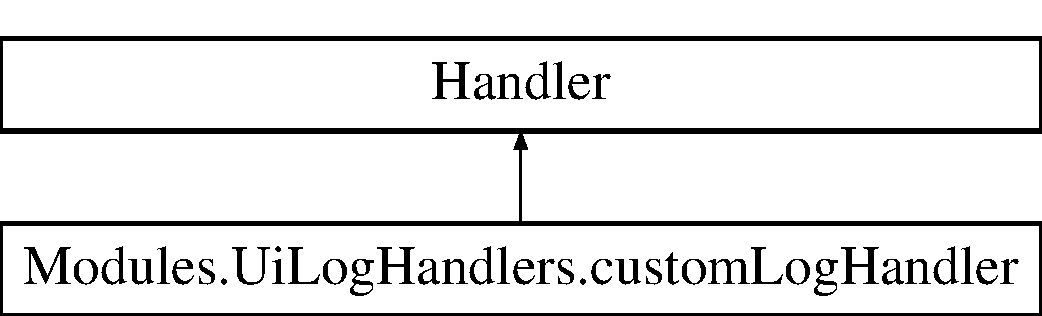
\includegraphics[height=2.000000cm]{classModules_1_1UiLogHandlers_1_1customLogHandler}
\end{center}
\end{figure}
\subsection*{Public Member Functions}
\begin{DoxyCompactItemize}
\item 
def \hyperlink{classModules_1_1UiLogHandlers_1_1customLogHandler_a516257c4da93f2937b47b38175e0fb0a}{\-\_\-\-\_\-init\-\_\-\-\_\-}
\item 
def \hyperlink{classModules_1_1UiLogHandlers_1_1customLogHandler_a333736c77b55367a1cbdc3150495bd87}{flush}
\item 
def \hyperlink{classModules_1_1UiLogHandlers_1_1customLogHandler_a9d276c9ecd8c566ad0bc10d5c516b793}{emit}
\end{DoxyCompactItemize}
\subsection*{Public Attributes}
\begin{DoxyCompactItemize}
\item 
\hypertarget{classModules_1_1UiLogHandlers_1_1customLogHandler_ab27011149cb953ba96d20bf97f9386dd}{{\bfseries log\-\_\-dialog}}\label{classModules_1_1UiLogHandlers_1_1customLogHandler_ab27011149cb953ba96d20bf97f9386dd}

\item 
\hypertarget{classModules_1_1UiLogHandlers_1_1customLogHandler_a6a5f60d2b7d13fe2381ce8bb101f1cda}{{\bfseries formatter}}\label{classModules_1_1UiLogHandlers_1_1customLogHandler_a6a5f60d2b7d13fe2381ce8bb101f1cda}

\item 
\hypertarget{classModules_1_1UiLogHandlers_1_1customLogHandler_a7d601145580a3a6daf9acbfcc2e5646a}{{\bfseries level}}\label{classModules_1_1UiLogHandlers_1_1customLogHandler_a7d601145580a3a6daf9acbfcc2e5646a}

\end{DoxyCompactItemize}


\subsection{Detailed Description}
\begin{DoxyVerb}Customloghandler, that handles log messages and emits them to the given 
LogWidget's log field. 
\end{DoxyVerb}
 

\subsection{Constructor \& Destructor Documentation}
\hypertarget{classModules_1_1UiLogHandlers_1_1customLogHandler_a516257c4da93f2937b47b38175e0fb0a}{\index{Modules\-::\-Ui\-Log\-Handlers\-::custom\-Log\-Handler@{Modules\-::\-Ui\-Log\-Handlers\-::custom\-Log\-Handler}!\-\_\-\-\_\-init\-\_\-\-\_\-@{\-\_\-\-\_\-init\-\_\-\-\_\-}}
\index{\-\_\-\-\_\-init\-\_\-\-\_\-@{\-\_\-\-\_\-init\-\_\-\-\_\-}!Modules::UiLogHandlers::customLogHandler@{Modules\-::\-Ui\-Log\-Handlers\-::custom\-Log\-Handler}}
\subsubsection[{\-\_\-\-\_\-init\-\_\-\-\_\-}]{\setlength{\rightskip}{0pt plus 5cm}def Modules.\-Ui\-Log\-Handlers.\-custom\-Log\-Handler.\-\_\-\-\_\-init\-\_\-\-\_\- (
\begin{DoxyParamCaption}
\item[{}]{self, }
\item[{}]{level, }
\item[{}]{formatter, }
\item[{}]{log\-\_\-dialog}
\end{DoxyParamCaption}
)}}\label{classModules_1_1UiLogHandlers_1_1customLogHandler_a516257c4da93f2937b47b38175e0fb0a}
\begin{DoxyVerb}Initializes the handler.

Args:
    level: The logging level set to this handler.
    formatter: The formatter set to this handler.
    log_dialog: The log dialog, which can add the message to the interface.
\end{DoxyVerb}
 

\subsection{Member Function Documentation}
\hypertarget{classModules_1_1UiLogHandlers_1_1customLogHandler_a9d276c9ecd8c566ad0bc10d5c516b793}{\index{Modules\-::\-Ui\-Log\-Handlers\-::custom\-Log\-Handler@{Modules\-::\-Ui\-Log\-Handlers\-::custom\-Log\-Handler}!emit@{emit}}
\index{emit@{emit}!Modules::UiLogHandlers::customLogHandler@{Modules\-::\-Ui\-Log\-Handlers\-::custom\-Log\-Handler}}
\subsubsection[{emit}]{\setlength{\rightskip}{0pt plus 5cm}def Modules.\-Ui\-Log\-Handlers.\-custom\-Log\-Handler.\-emit (
\begin{DoxyParamCaption}
\item[{}]{self, }
\item[{}]{record}
\end{DoxyParamCaption}
)}}\label{classModules_1_1UiLogHandlers_1_1customLogHandler_a9d276c9ecd8c566ad0bc10d5c516b793}
\begin{DoxyVerb}Emits the log message to the destination, which is set when the handler 
is initialized.

Args:
    record: The record which will be emitted.
\end{DoxyVerb}
 \hypertarget{classModules_1_1UiLogHandlers_1_1customLogHandler_a333736c77b55367a1cbdc3150495bd87}{\index{Modules\-::\-Ui\-Log\-Handlers\-::custom\-Log\-Handler@{Modules\-::\-Ui\-Log\-Handlers\-::custom\-Log\-Handler}!flush@{flush}}
\index{flush@{flush}!Modules::UiLogHandlers::customLogHandler@{Modules\-::\-Ui\-Log\-Handlers\-::custom\-Log\-Handler}}
\subsubsection[{flush}]{\setlength{\rightskip}{0pt plus 5cm}def Modules.\-Ui\-Log\-Handlers.\-custom\-Log\-Handler.\-flush (
\begin{DoxyParamCaption}
\item[{}]{self}
\end{DoxyParamCaption}
)}}\label{classModules_1_1UiLogHandlers_1_1customLogHandler_a333736c77b55367a1cbdc3150495bd87}
\begin{DoxyVerb}Does nothing here, has to be here because this is inherited.
\end{DoxyVerb}
 

The documentation for this class was generated from the following file\-:\begin{DoxyCompactItemize}
\item 
Modules/Ui\-Log\-Handlers.\-py\end{DoxyCompactItemize}

\hypertarget{classModules_1_1CutFile_1_1CutFile}{\section{Modules.\-Cut\-File.\-Cut\-File Class Reference}
\label{classModules_1_1CutFile_1_1CutFile}\index{Modules.\-Cut\-File.\-Cut\-File@{Modules.\-Cut\-File.\-Cut\-File}}
}
\subsection*{Public Member Functions}
\begin{DoxyCompactItemize}
\item 
def \hyperlink{classModules_1_1CutFile_1_1CutFile_a77f945f7b5806ad366101621cf0f1090}{\-\_\-\-\_\-init\-\_\-\-\_\-}
\item 
def \hyperlink{classModules_1_1CutFile_1_1CutFile_abbefde5e9218868e815110a427b89f82}{set\-\_\-info}
\item 
def \hyperlink{classModules_1_1CutFile_1_1CutFile_a3e74135fa738e9fbee272b0cb3c4c560}{load\-\_\-file}
\item 
def \hyperlink{classModules_1_1CutFile_1_1CutFile_a1b5dd6971e91ee35f8a7a432410fd9d1}{save}
\item 
def \hyperlink{classModules_1_1CutFile_1_1CutFile_acdb33341563b9a0806c02e2566a0dbdb}{split}
\item 
def \hyperlink{classModules_1_1CutFile_1_1CutFile_a69f3dc0b72f13193d66fbb2d672bb7e7}{copy\-\_\-info}
\end{DoxyCompactItemize}
\subsection*{Public Attributes}
\begin{DoxyCompactItemize}
\item 
\hypertarget{classModules_1_1CutFile_1_1CutFile_ae70d0e702c9f26e66484088031b88dfd}{{\bfseries directory}}\label{classModules_1_1CutFile_1_1CutFile_ae70d0e702c9f26e66484088031b88dfd}

\item 
\hypertarget{classModules_1_1CutFile_1_1CutFile_af94284e2ae1f1f1cddedb155cef2e217}{{\bfseries element}}\label{classModules_1_1CutFile_1_1CutFile_af94284e2ae1f1f1cddedb155cef2e217}

\item 
\hypertarget{classModules_1_1CutFile_1_1CutFile_aca8ea127fcd91c459b722bf2a1f890e2}{{\bfseries count}}\label{classModules_1_1CutFile_1_1CutFile_aca8ea127fcd91c459b722bf2a1f890e2}

\item 
\hypertarget{classModules_1_1CutFile_1_1CutFile_ae210d76ac22c4fc8ef0479536c96968f}{{\bfseries is\-\_\-elem\-\_\-loss}}\label{classModules_1_1CutFile_1_1CutFile_ae210d76ac22c4fc8ef0479536c96968f}

\item 
\hypertarget{classModules_1_1CutFile_1_1CutFile_acd632dd3f3dd6a720fc18dbc888a81f9}{{\bfseries split\-\_\-number}}\label{classModules_1_1CutFile_1_1CutFile_acd632dd3f3dd6a720fc18dbc888a81f9}

\item 
\hypertarget{classModules_1_1CutFile_1_1CutFile_aadf1d693dc354cde0ecdf68918e07069}{{\bfseries split\-\_\-count}}\label{classModules_1_1CutFile_1_1CutFile_aadf1d693dc354cde0ecdf68918e07069}

\item 
\hypertarget{classModules_1_1CutFile_1_1CutFile_a119dc055fec0e49c046b2cf67b4fef7f}{{\bfseries type}}\label{classModules_1_1CutFile_1_1CutFile_a119dc055fec0e49c046b2cf67b4fef7f}

\item 
\hypertarget{classModules_1_1CutFile_1_1CutFile_a8c06d313004ef8a37e422f27447b4391}{{\bfseries weight\-\_\-factor}}\label{classModules_1_1CutFile_1_1CutFile_a8c06d313004ef8a37e422f27447b4391}

\item 
\hypertarget{classModules_1_1CutFile_1_1CutFile_a711bd9e2ff10367af152b999dd183361}{{\bfseries energy}}\label{classModules_1_1CutFile_1_1CutFile_a711bd9e2ff10367af152b999dd183361}

\item 
\hypertarget{classModules_1_1CutFile_1_1CutFile_a9303581407c0166d7d560641fecdb5be}{{\bfseries detector\-\_\-angle}}\label{classModules_1_1CutFile_1_1CutFile_a9303581407c0166d7d560641fecdb5be}

\item 
\hypertarget{classModules_1_1CutFile_1_1CutFile_a853145c4268a367383beef002dded059}{{\bfseries element\-\_\-scatter}}\label{classModules_1_1CutFile_1_1CutFile_a853145c4268a367383beef002dded059}

\item 
\hypertarget{classModules_1_1CutFile_1_1CutFile_af06381681f43c69725fa30f1877f0492}{{\bfseries data}}\label{classModules_1_1CutFile_1_1CutFile_af06381681f43c69725fa30f1877f0492}

\item 
\hypertarget{classModules_1_1CutFile_1_1CutFile_ac26f41b6984a82b8d4fbe86ae11b9f65}{{\bfseries element\-\_\-number}}\label{classModules_1_1CutFile_1_1CutFile_ac26f41b6984a82b8d4fbe86ae11b9f65}

\end{DoxyCompactItemize}


\subsection{Detailed Description}
\begin{DoxyVerb}Cut file_path object for when reading cut files is necessary.
\end{DoxyVerb}
 

\subsection{Constructor \& Destructor Documentation}
\hypertarget{classModules_1_1CutFile_1_1CutFile_a77f945f7b5806ad366101621cf0f1090}{\index{Modules\-::\-Cut\-File\-::\-Cut\-File@{Modules\-::\-Cut\-File\-::\-Cut\-File}!\-\_\-\-\_\-init\-\_\-\-\_\-@{\-\_\-\-\_\-init\-\_\-\-\_\-}}
\index{\-\_\-\-\_\-init\-\_\-\-\_\-@{\-\_\-\-\_\-init\-\_\-\-\_\-}!Modules::CutFile::CutFile@{Modules\-::\-Cut\-File\-::\-Cut\-File}}
\subsubsection[{\-\_\-\-\_\-init\-\_\-\-\_\-}]{\setlength{\rightskip}{0pt plus 5cm}def Modules.\-Cut\-File.\-Cut\-File.\-\_\-\-\_\-init\-\_\-\-\_\- (
\begin{DoxyParamCaption}
\item[{}]{self, }
\item[{}]{directory = {\ttfamily None}, }
\item[{}]{elem\-\_\-loss = {\ttfamily False}, }
\item[{}]{weight\-\_\-factor = {\ttfamily 1.0}, }
\item[{}]{split\-\_\-number = {\ttfamily 0}, }
\item[{}]{split\-\_\-count = {\ttfamily 1}}
\end{DoxyParamCaption}
)}}\label{classModules_1_1CutFile_1_1CutFile_a77f945f7b5806ad366101621cf0f1090}
\begin{DoxyVerb}Inits cut file_path object.

Args:
    directory: String representing cut directory.
    elem_loss: Boolean representing whether cut file_path is made from
       elemental losses splits.
    weight_factor: Float representing element weight factor. 
    split_number: Integer. Required for Elemental Losses, do not overwrite
          splits.
    split_count: Integer. Required for Elemental Losses, total count of 
         splits.
\end{DoxyVerb}
 

\subsection{Member Function Documentation}
\hypertarget{classModules_1_1CutFile_1_1CutFile_a69f3dc0b72f13193d66fbb2d672bb7e7}{\index{Modules\-::\-Cut\-File\-::\-Cut\-File@{Modules\-::\-Cut\-File\-::\-Cut\-File}!copy\-\_\-info@{copy\-\_\-info}}
\index{copy\-\_\-info@{copy\-\_\-info}!Modules::CutFile::CutFile@{Modules\-::\-Cut\-File\-::\-Cut\-File}}
\subsubsection[{copy\-\_\-info}]{\setlength{\rightskip}{0pt plus 5cm}def Modules.\-Cut\-File.\-Cut\-File.\-copy\-\_\-info (
\begin{DoxyParamCaption}
\item[{}]{self, }
\item[{}]{cut\-\_\-file, }
\item[{}]{data, }
\item[{}]{additional\-\_\-weight\-\_\-factor = {\ttfamily 1.0}}
\end{DoxyParamCaption}
)}}\label{classModules_1_1CutFile_1_1CutFile_a69f3dc0b72f13193d66fbb2d672bb7e7}
\begin{DoxyVerb}Copy information from cut file_path object into this.

Args:
    cut_file: CutFile class object.
    data: List of data points.
    additional_weight_factor: Float
\end{DoxyVerb}
 \hypertarget{classModules_1_1CutFile_1_1CutFile_a3e74135fa738e9fbee272b0cb3c4c560}{\index{Modules\-::\-Cut\-File\-::\-Cut\-File@{Modules\-::\-Cut\-File\-::\-Cut\-File}!load\-\_\-file@{load\-\_\-file}}
\index{load\-\_\-file@{load\-\_\-file}!Modules::CutFile::CutFile@{Modules\-::\-Cut\-File\-::\-Cut\-File}}
\subsubsection[{load\-\_\-file}]{\setlength{\rightskip}{0pt plus 5cm}def Modules.\-Cut\-File.\-Cut\-File.\-load\-\_\-file (
\begin{DoxyParamCaption}
\item[{}]{self, }
\item[{}]{file}
\end{DoxyParamCaption}
)}}\label{classModules_1_1CutFile_1_1CutFile_a3e74135fa738e9fbee272b0cb3c4c560}
\begin{DoxyVerb}Load and parse cut file_path.

Args:
    file: String representing cut file.
\end{DoxyVerb}
 \hypertarget{classModules_1_1CutFile_1_1CutFile_a1b5dd6971e91ee35f8a7a432410fd9d1}{\index{Modules\-::\-Cut\-File\-::\-Cut\-File@{Modules\-::\-Cut\-File\-::\-Cut\-File}!save@{save}}
\index{save@{save}!Modules::CutFile::CutFile@{Modules\-::\-Cut\-File\-::\-Cut\-File}}
\subsubsection[{save}]{\setlength{\rightskip}{0pt plus 5cm}def Modules.\-Cut\-File.\-Cut\-File.\-save (
\begin{DoxyParamCaption}
\item[{}]{self, }
\item[{}]{element\-\_\-count = {\ttfamily 0}}
\end{DoxyParamCaption}
)}}\label{classModules_1_1CutFile_1_1CutFile_a1b5dd6971e91ee35f8a7a432410fd9d1}
\begin{DoxyVerb}Save cut file_path.

Saves data points into cut file_path with meta information.

Args:
    element_count: Integer representing which selection was used of total
           count of same element and isotope selection. This is so
           that we do not overwrite first 2H selection with other
           2H selection.
\end{DoxyVerb}
 \hypertarget{classModules_1_1CutFile_1_1CutFile_abbefde5e9218868e815110a427b89f82}{\index{Modules\-::\-Cut\-File\-::\-Cut\-File@{Modules\-::\-Cut\-File\-::\-Cut\-File}!set\-\_\-info@{set\-\_\-info}}
\index{set\-\_\-info@{set\-\_\-info}!Modules::CutFile::CutFile@{Modules\-::\-Cut\-File\-::\-Cut\-File}}
\subsubsection[{set\-\_\-info}]{\setlength{\rightskip}{0pt plus 5cm}def Modules.\-Cut\-File.\-Cut\-File.\-set\-\_\-info (
\begin{DoxyParamCaption}
\item[{}]{self, }
\item[{}]{selection, }
\item[{}]{data}
\end{DoxyParamCaption}
)}}\label{classModules_1_1CutFile_1_1CutFile_abbefde5e9218868e815110a427b89f82}
\begin{DoxyVerb}Set selection information and data into CutFile.

Args:
    selection: Selection class object.
    data: Lists of data points.
\end{DoxyVerb}
 \hypertarget{classModules_1_1CutFile_1_1CutFile_acdb33341563b9a0806c02e2566a0dbdb}{\index{Modules\-::\-Cut\-File\-::\-Cut\-File@{Modules\-::\-Cut\-File\-::\-Cut\-File}!split@{split}}
\index{split@{split}!Modules::CutFile::CutFile@{Modules\-::\-Cut\-File\-::\-Cut\-File}}
\subsubsection[{split}]{\setlength{\rightskip}{0pt plus 5cm}def Modules.\-Cut\-File.\-Cut\-File.\-split (
\begin{DoxyParamCaption}
\item[{}]{self, }
\item[{}]{reference\-\_\-cut, }
\item[{}]{splits = {\ttfamily 10}, }
\item[{}]{save = {\ttfamily True}}
\end{DoxyParamCaption}
)}}\label{classModules_1_1CutFile_1_1CutFile_acdb33341563b9a0806c02e2566a0dbdb}
\begin{DoxyVerb}Splits cut file into X splits based on reference cut.

Args:
    reference_cut: Cut file (of heavy element) which is used split.
    splits: Integer determining how many splits is cut splitted to.
    save: Boolean deciding whether or not to save splits.
    
Return:
    Returns a list containing lists of the cut's splits' values.
\end{DoxyVerb}
 

The documentation for this class was generated from the following file\-:\begin{DoxyCompactItemize}
\item 
Modules/Cut\-File.\-py\end{DoxyCompactItemize}

\hypertarget{classModules_1_1DepthFiles_1_1DepthFiles}{\section{Modules.\-Depth\-Files.\-Depth\-Files Class Reference}
\label{classModules_1_1DepthFiles_1_1DepthFiles}\index{Modules.\-Depth\-Files.\-Depth\-Files@{Modules.\-Depth\-Files.\-Depth\-Files}}
}
Inheritance diagram for Modules.\-Depth\-Files.\-Depth\-Files\-:\begin{figure}[H]
\begin{center}
\leavevmode
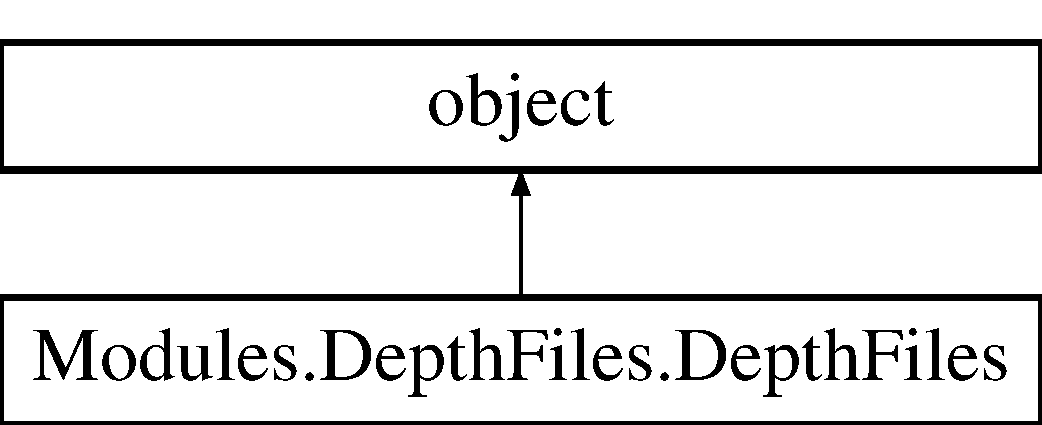
\includegraphics[height=2.000000cm]{classModules_1_1DepthFiles_1_1DepthFiles}
\end{center}
\end{figure}
\subsection*{Public Member Functions}
\begin{DoxyCompactItemize}
\item 
def \hyperlink{classModules_1_1DepthFiles_1_1DepthFiles_a1b9bf9c184949775ff1cf8372f2dc3d6}{\-\_\-\-\_\-init\-\_\-\-\_\-}
\item 
def \hyperlink{classModules_1_1DepthFiles_1_1DepthFiles_ac5e61061ced613567796cfc7e84e13af}{create\-\_\-depth\-\_\-files}
\end{DoxyCompactItemize}
\subsection*{Public Attributes}
\begin{DoxyCompactItemize}
\item 
\hypertarget{classModules_1_1DepthFiles_1_1DepthFiles_ac3281cfac36e109a357d5ce6b810cded}{{\bfseries bin\-\_\-dir}}\label{classModules_1_1DepthFiles_1_1DepthFiles_ac3281cfac36e109a357d5ce6b810cded}

\item 
\hypertarget{classModules_1_1DepthFiles_1_1DepthFiles_a2d177607b373b564c2285acede124a6f}{{\bfseries command\-\_\-win}}\label{classModules_1_1DepthFiles_1_1DepthFiles_a2d177607b373b564c2285acede124a6f}

\item 
\hypertarget{classModules_1_1DepthFiles_1_1DepthFiles_a030a740044fd055eeb09223ac3a75d69}{{\bfseries command\-\_\-unix}}\label{classModules_1_1DepthFiles_1_1DepthFiles_a030a740044fd055eeb09223ac3a75d69}

\end{DoxyCompactItemize}


\subsection{Detailed Description}
\begin{DoxyVerb}DepthFiles handles calling the external programs to create depth files.
\end{DoxyVerb}
 

\subsection{Constructor \& Destructor Documentation}
\hypertarget{classModules_1_1DepthFiles_1_1DepthFiles_a1b9bf9c184949775ff1cf8372f2dc3d6}{\index{Modules\-::\-Depth\-Files\-::\-Depth\-Files@{Modules\-::\-Depth\-Files\-::\-Depth\-Files}!\-\_\-\-\_\-init\-\_\-\-\_\-@{\-\_\-\-\_\-init\-\_\-\-\_\-}}
\index{\-\_\-\-\_\-init\-\_\-\-\_\-@{\-\_\-\-\_\-init\-\_\-\-\_\-}!Modules::DepthFiles::DepthFiles@{Modules\-::\-Depth\-Files\-::\-Depth\-Files}}
\subsubsection[{\-\_\-\-\_\-init\-\_\-\-\_\-}]{\setlength{\rightskip}{0pt plus 5cm}def Modules.\-Depth\-Files.\-Depth\-Files.\-\_\-\-\_\-init\-\_\-\-\_\- (
\begin{DoxyParamCaption}
\item[{}]{self, }
\item[{}]{filepaths, }
\item[{}]{outputpath}
\end{DoxyParamCaption}
)}}\label{classModules_1_1DepthFiles_1_1DepthFiles_a1b9bf9c184949775ff1cf8372f2dc3d6}
\begin{DoxyVerb}Inits DepthFiles.

Args:
    filepaths: Full paths of cutfiles to be used.
    outputpath: Full path of where depth files are to be created.
\end{DoxyVerb}
 

\subsection{Member Function Documentation}
\hypertarget{classModules_1_1DepthFiles_1_1DepthFiles_ac5e61061ced613567796cfc7e84e13af}{\index{Modules\-::\-Depth\-Files\-::\-Depth\-Files@{Modules\-::\-Depth\-Files\-::\-Depth\-Files}!create\-\_\-depth\-\_\-files@{create\-\_\-depth\-\_\-files}}
\index{create\-\_\-depth\-\_\-files@{create\-\_\-depth\-\_\-files}!Modules::DepthFiles::DepthFiles@{Modules\-::\-Depth\-Files\-::\-Depth\-Files}}
\subsubsection[{create\-\_\-depth\-\_\-files}]{\setlength{\rightskip}{0pt plus 5cm}def Modules.\-Depth\-Files.\-Depth\-Files.\-create\-\_\-depth\-\_\-files (
\begin{DoxyParamCaption}
\item[{}]{self}
\end{DoxyParamCaption}
)}}\label{classModules_1_1DepthFiles_1_1DepthFiles_ac5e61061ced613567796cfc7e84e13af}
\begin{DoxyVerb}Generate the files necessary for drawing the depth profile
\end{DoxyVerb}
 

The documentation for this class was generated from the following file\-:\begin{DoxyCompactItemize}
\item 
Modules/Depth\-Files.\-py\end{DoxyCompactItemize}

\hypertarget{classDialogs_1_1DepthProfileDialog_1_1DepthProfileDialog}{\section{Dialogs.\-Depth\-Profile\-Dialog.\-Depth\-Profile\-Dialog Class Reference}
\label{classDialogs_1_1DepthProfileDialog_1_1DepthProfileDialog}\index{Dialogs.\-Depth\-Profile\-Dialog.\-Depth\-Profile\-Dialog@{Dialogs.\-Depth\-Profile\-Dialog.\-Depth\-Profile\-Dialog}}
}
Inheritance diagram for Dialogs.\-Depth\-Profile\-Dialog.\-Depth\-Profile\-Dialog\-:\begin{figure}[H]
\begin{center}
\leavevmode
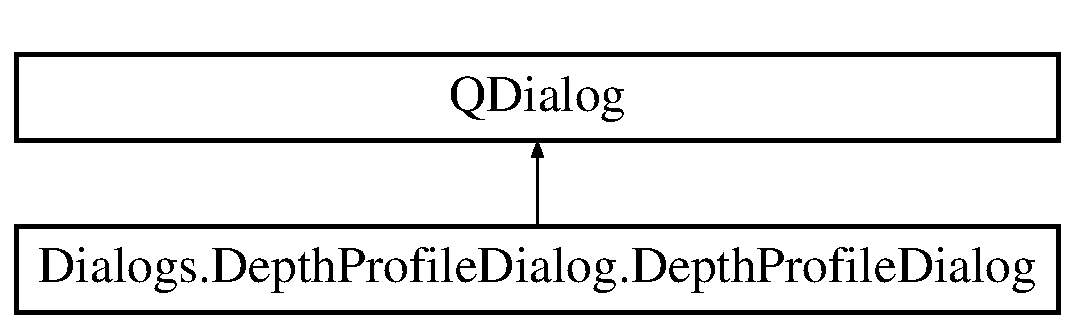
\includegraphics[height=2.000000cm]{classDialogs_1_1DepthProfileDialog_1_1DepthProfileDialog}
\end{center}
\end{figure}
\subsection*{Public Member Functions}
\begin{DoxyCompactItemize}
\item 
def \hyperlink{classDialogs_1_1DepthProfileDialog_1_1DepthProfileDialog_a4caa83268490c73b1e7dc6a645f7282f}{\-\_\-\-\_\-init\-\_\-\-\_\-}
\end{DoxyCompactItemize}
\subsection*{Public Attributes}
\begin{DoxyCompactItemize}
\item 
\hypertarget{classDialogs_1_1DepthProfileDialog_1_1DepthProfileDialog_ae56f240cae99a2e587e35694bab3cde8}{{\bfseries parent}}\label{classDialogs_1_1DepthProfileDialog_1_1DepthProfileDialog_ae56f240cae99a2e587e35694bab3cde8}

\item 
\hypertarget{classDialogs_1_1DepthProfileDialog_1_1DepthProfileDialog_a26b6f749f5342f7739c8864708d9a887}{{\bfseries ui}}\label{classDialogs_1_1DepthProfileDialog_1_1DepthProfileDialog_a26b6f749f5342f7739c8864708d9a887}

\item 
\hypertarget{classDialogs_1_1DepthProfileDialog_1_1DepthProfileDialog_af4c3f3175238254743d40c8a80cc5f01}{{\bfseries measurement}}\label{classDialogs_1_1DepthProfileDialog_1_1DepthProfileDialog_af4c3f3175238254743d40c8a80cc5f01}

\end{DoxyCompactItemize}
\subsection*{Static Public Attributes}
\begin{DoxyCompactItemize}
\item 
\hypertarget{classDialogs_1_1DepthProfileDialog_1_1DepthProfileDialog_adbb39f89a5f3aa9eb6046653096c9937}{dictionary {\bfseries checked\-\_\-cuts} = \{\}}\label{classDialogs_1_1DepthProfileDialog_1_1DepthProfileDialog_adbb39f89a5f3aa9eb6046653096c9937}

\item 
\hypertarget{classDialogs_1_1DepthProfileDialog_1_1DepthProfileDialog_a1e733f52ab566af18aba810af495fad2}{string {\bfseries x\-\_\-unit} = \char`\"{}1e15 at./cm²\char`\"{}}\label{classDialogs_1_1DepthProfileDialog_1_1DepthProfileDialog_a1e733f52ab566af18aba810af495fad2}

\item 
\hypertarget{classDialogs_1_1DepthProfileDialog_1_1DepthProfileDialog_af22edb5f50dc70ec735c60d0063e8814}{{\bfseries line\-\_\-zero} = False}\label{classDialogs_1_1DepthProfileDialog_1_1DepthProfileDialog_af22edb5f50dc70ec735c60d0063e8814}

\item 
\hypertarget{classDialogs_1_1DepthProfileDialog_1_1DepthProfileDialog_a598a2ec3c25fcc09b1bd18b75c034cb2}{{\bfseries line\-\_\-scale} = False}\label{classDialogs_1_1DepthProfileDialog_1_1DepthProfileDialog_a598a2ec3c25fcc09b1bd18b75c034cb2}

\item 
\hypertarget{classDialogs_1_1DepthProfileDialog_1_1DepthProfileDialog_acfc4509e20de3e41dd19d3365dfce50b}{float {\bfseries systerr} = 0.\-0}\label{classDialogs_1_1DepthProfileDialog_1_1DepthProfileDialog_acfc4509e20de3e41dd19d3365dfce50b}

\end{DoxyCompactItemize}


\subsection{Constructor \& Destructor Documentation}
\hypertarget{classDialogs_1_1DepthProfileDialog_1_1DepthProfileDialog_a4caa83268490c73b1e7dc6a645f7282f}{\index{Dialogs\-::\-Depth\-Profile\-Dialog\-::\-Depth\-Profile\-Dialog@{Dialogs\-::\-Depth\-Profile\-Dialog\-::\-Depth\-Profile\-Dialog}!\-\_\-\-\_\-init\-\_\-\-\_\-@{\-\_\-\-\_\-init\-\_\-\-\_\-}}
\index{\-\_\-\-\_\-init\-\_\-\-\_\-@{\-\_\-\-\_\-init\-\_\-\-\_\-}!Dialogs::DepthProfileDialog::DepthProfileDialog@{Dialogs\-::\-Depth\-Profile\-Dialog\-::\-Depth\-Profile\-Dialog}}
\subsubsection[{\-\_\-\-\_\-init\-\_\-\-\_\-}]{\setlength{\rightskip}{0pt plus 5cm}def Dialogs.\-Depth\-Profile\-Dialog.\-Depth\-Profile\-Dialog.\-\_\-\-\_\-init\-\_\-\-\_\- (
\begin{DoxyParamCaption}
\item[{}]{self, }
\item[{}]{parent}
\end{DoxyParamCaption}
)}}\label{classDialogs_1_1DepthProfileDialog_1_1DepthProfileDialog_a4caa83268490c73b1e7dc6a645f7282f}
\begin{DoxyVerb}Inits depth profile dialog

Args:
    parent: MeasurementTabWidget
\end{DoxyVerb}
 

The documentation for this class was generated from the following file\-:\begin{DoxyCompactItemize}
\item 
Dialogs/Depth\-Profile\-Dialog.\-py\end{DoxyCompactItemize}

\hypertarget{classDialogs_1_1DepthProfileIgnoreElements_1_1DepthProfileIgnoreElements}{\section{Dialogs.\-Depth\-Profile\-Ignore\-Elements.\-Depth\-Profile\-Ignore\-Elements Class Reference}
\label{classDialogs_1_1DepthProfileIgnoreElements_1_1DepthProfileIgnoreElements}\index{Dialogs.\-Depth\-Profile\-Ignore\-Elements.\-Depth\-Profile\-Ignore\-Elements@{Dialogs.\-Depth\-Profile\-Ignore\-Elements.\-Depth\-Profile\-Ignore\-Elements}}
}
Inheritance diagram for Dialogs.\-Depth\-Profile\-Ignore\-Elements.\-Depth\-Profile\-Ignore\-Elements\-:\begin{figure}[H]
\begin{center}
\leavevmode
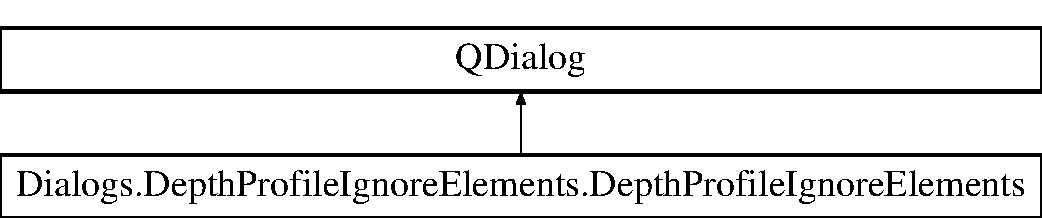
\includegraphics[height=2.000000cm]{classDialogs_1_1DepthProfileIgnoreElements_1_1DepthProfileIgnoreElements}
\end{center}
\end{figure}
\subsection*{Public Member Functions}
\begin{DoxyCompactItemize}
\item 
def \hyperlink{classDialogs_1_1DepthProfileIgnoreElements_1_1DepthProfileIgnoreElements_a2c18d10b3c4462bb79816395b9518167}{\-\_\-\-\_\-init\-\_\-\-\_\-}
\end{DoxyCompactItemize}
\subsection*{Public Attributes}
\begin{DoxyCompactItemize}
\item 
\hypertarget{classDialogs_1_1DepthProfileIgnoreElements_1_1DepthProfileIgnoreElements_a3d157c0d198e9ac56a4b4af54912f11b}{{\bfseries ignore\-\_\-from\-\_\-graph}}\label{classDialogs_1_1DepthProfileIgnoreElements_1_1DepthProfileIgnoreElements_a3d157c0d198e9ac56a4b4af54912f11b}

\item 
\hypertarget{classDialogs_1_1DepthProfileIgnoreElements_1_1DepthProfileIgnoreElements_aa31c4b1d733784ddb515f79a75740a0e}{{\bfseries ignore\-\_\-from\-\_\-ratio}}\label{classDialogs_1_1DepthProfileIgnoreElements_1_1DepthProfileIgnoreElements_aa31c4b1d733784ddb515f79a75740a0e}

\end{DoxyCompactItemize}


\subsection{Constructor \& Destructor Documentation}
\hypertarget{classDialogs_1_1DepthProfileIgnoreElements_1_1DepthProfileIgnoreElements_a2c18d10b3c4462bb79816395b9518167}{\index{Dialogs\-::\-Depth\-Profile\-Ignore\-Elements\-::\-Depth\-Profile\-Ignore\-Elements@{Dialogs\-::\-Depth\-Profile\-Ignore\-Elements\-::\-Depth\-Profile\-Ignore\-Elements}!\-\_\-\-\_\-init\-\_\-\-\_\-@{\-\_\-\-\_\-init\-\_\-\-\_\-}}
\index{\-\_\-\-\_\-init\-\_\-\-\_\-@{\-\_\-\-\_\-init\-\_\-\-\_\-}!Dialogs::DepthProfileIgnoreElements::DepthProfileIgnoreElements@{Dialogs\-::\-Depth\-Profile\-Ignore\-Elements\-::\-Depth\-Profile\-Ignore\-Elements}}
\subsubsection[{\-\_\-\-\_\-init\-\_\-\-\_\-}]{\setlength{\rightskip}{0pt plus 5cm}def Dialogs.\-Depth\-Profile\-Ignore\-Elements.\-Depth\-Profile\-Ignore\-Elements.\-\_\-\-\_\-init\-\_\-\-\_\- (
\begin{DoxyParamCaption}
\item[{}]{self, }
\item[{}]{elements, }
\item[{}]{ignored\-\_\-graph, }
\item[{}]{ignored\-\_\-ratio}
\end{DoxyParamCaption}
)}}\label{classDialogs_1_1DepthProfileIgnoreElements_1_1DepthProfileIgnoreElements_a2c18d10b3c4462bb79816395b9518167}
\begin{DoxyVerb}Init the dialog.

Args:
    elements: A list of elements in Depth Profile.
    ignored_graph: A list of elements ignored previously for the graph.
    ignored_ratio: A list of elements ignored previously for ratio
           calculation.
\end{DoxyVerb}
 

The documentation for this class was generated from the following file\-:\begin{DoxyCompactItemize}
\item 
Dialogs/Depth\-Profile\-Ignore\-Elements.\-py\end{DoxyCompactItemize}

\hypertarget{classModules_1_1DepthProfileSettings_1_1DepthProfileSettings}{\section{Modules.\-Depth\-Profile\-Settings.\-Depth\-Profile\-Settings Class Reference}
\label{classModules_1_1DepthProfileSettings_1_1DepthProfileSettings}\index{Modules.\-Depth\-Profile\-Settings.\-Depth\-Profile\-Settings@{Modules.\-Depth\-Profile\-Settings.\-Depth\-Profile\-Settings}}
}
\subsection*{Public Member Functions}
\begin{DoxyCompactItemize}
\item 
def \hyperlink{classModules_1_1DepthProfileSettings_1_1DepthProfileSettings_a65f273bdb7d9184fd81a2838aa905d40}{\-\_\-\-\_\-init\-\_\-\-\_\-}
\item 
def \hyperlink{classModules_1_1DepthProfileSettings_1_1DepthProfileSettings_a750fe5ee358369650f1b1e2966168225}{show}
\item 
def \hyperlink{classModules_1_1DepthProfileSettings_1_1DepthProfileSettings_a076a13d49766fc146e7c23575e446a8f}{set\-\_\-settings}
\item 
def \hyperlink{classModules_1_1DepthProfileSettings_1_1DepthProfileSettings_a6a91db400bb429e91771092f88c96389}{load\-\_\-settings}
\item 
def \hyperlink{classModules_1_1DepthProfileSettings_1_1DepthProfileSettings_aa7d5e07e945a2902bf52976dacab77c0}{save\-\_\-settings}
\end{DoxyCompactItemize}
\subsection*{Public Attributes}
\begin{DoxyCompactItemize}
\item 
\hypertarget{classModules_1_1DepthProfileSettings_1_1DepthProfileSettings_ac6c00635ff349b09bafc8661afa878ea}{{\bfseries depth\-\_\-profile\-\_\-settings\-\_\-filename}}\label{classModules_1_1DepthProfileSettings_1_1DepthProfileSettings_ac6c00635ff349b09bafc8661afa878ea}

\item 
\hypertarget{classModules_1_1DepthProfileSettings_1_1DepthProfileSettings_a0608b7bdbaf0734b70dafc0392622a65}{{\bfseries config}}\label{classModules_1_1DepthProfileSettings_1_1DepthProfileSettings_a0608b7bdbaf0734b70dafc0392622a65}

\item 
\hypertarget{classModules_1_1DepthProfileSettings_1_1DepthProfileSettings_a9810c25f152cc137e5e4bdcf72347274}{{\bfseries use\-\_\-settings}}\label{classModules_1_1DepthProfileSettings_1_1DepthProfileSettings_a9810c25f152cc137e5e4bdcf72347274}

\item 
\hypertarget{classModules_1_1DepthProfileSettings_1_1DepthProfileSettings_a902fa23e25195dd6a7585251e72a9dca}{{\bfseries number\-\_\-of\-\_\-depth\-\_\-steps}}\label{classModules_1_1DepthProfileSettings_1_1DepthProfileSettings_a902fa23e25195dd6a7585251e72a9dca}

\item 
\hypertarget{classModules_1_1DepthProfileSettings_1_1DepthProfileSettings_adf63bbe7d11cfc669af4b49391462484}{{\bfseries depth\-\_\-step\-\_\-for\-\_\-stopping}}\label{classModules_1_1DepthProfileSettings_1_1DepthProfileSettings_adf63bbe7d11cfc669af4b49391462484}

\item 
\hypertarget{classModules_1_1DepthProfileSettings_1_1DepthProfileSettings_abf37b200476fa7fc818640d782a4d0d9}{{\bfseries depth\-\_\-step\-\_\-for\-\_\-output}}\label{classModules_1_1DepthProfileSettings_1_1DepthProfileSettings_abf37b200476fa7fc818640d782a4d0d9}

\item 
\hypertarget{classModules_1_1DepthProfileSettings_1_1DepthProfileSettings_a5b2b52f2680bb3dae49b9afbffec8fe8}{{\bfseries depths\-\_\-for\-\_\-concentration\-\_\-from}}\label{classModules_1_1DepthProfileSettings_1_1DepthProfileSettings_a5b2b52f2680bb3dae49b9afbffec8fe8}

\item 
\hypertarget{classModules_1_1DepthProfileSettings_1_1DepthProfileSettings_a9c52a32577e8628bd91a5836e5faa71d}{{\bfseries depths\-\_\-for\-\_\-concentration\-\_\-to}}\label{classModules_1_1DepthProfileSettings_1_1DepthProfileSettings_a9c52a32577e8628bd91a5836e5faa71d}

\item 
\hypertarget{classModules_1_1DepthProfileSettings_1_1DepthProfileSettings_aa9cb2c3a112b51aeac71ed1040fa96e2}{{\bfseries filepath}}\label{classModules_1_1DepthProfileSettings_1_1DepthProfileSettings_aa9cb2c3a112b51aeac71ed1040fa96e2}

\end{DoxyCompactItemize}


\subsection{Detailed Description}
\begin{DoxyVerb}DepthProfileSettings holds the all project specific measurement unit parameters.
\end{DoxyVerb}
 

\subsection{Constructor \& Destructor Documentation}
\hypertarget{classModules_1_1DepthProfileSettings_1_1DepthProfileSettings_a65f273bdb7d9184fd81a2838aa905d40}{\index{Modules\-::\-Depth\-Profile\-Settings\-::\-Depth\-Profile\-Settings@{Modules\-::\-Depth\-Profile\-Settings\-::\-Depth\-Profile\-Settings}!\-\_\-\-\_\-init\-\_\-\-\_\-@{\-\_\-\-\_\-init\-\_\-\-\_\-}}
\index{\-\_\-\-\_\-init\-\_\-\-\_\-@{\-\_\-\-\_\-init\-\_\-\-\_\-}!Modules::DepthProfileSettings::DepthProfileSettings@{Modules\-::\-Depth\-Profile\-Settings\-::\-Depth\-Profile\-Settings}}
\subsubsection[{\-\_\-\-\_\-init\-\_\-\-\_\-}]{\setlength{\rightskip}{0pt plus 5cm}def Modules.\-Depth\-Profile\-Settings.\-Depth\-Profile\-Settings.\-\_\-\-\_\-init\-\_\-\-\_\- (
\begin{DoxyParamCaption}
\item[{}]{self, }
\item[{}]{settings\-\_\-filepath = {\ttfamily None}}
\end{DoxyParamCaption}
)}}\label{classModules_1_1DepthProfileSettings_1_1DepthProfileSettings_a65f273bdb7d9184fd81a2838aa905d40}
\begin{DoxyVerb}Inits DepthProfileSettings.

Args:
    settings_filepath: filepath for the settings file to be loaded
\end{DoxyVerb}
 

\subsection{Member Function Documentation}
\hypertarget{classModules_1_1DepthProfileSettings_1_1DepthProfileSettings_a6a91db400bb429e91771092f88c96389}{\index{Modules\-::\-Depth\-Profile\-Settings\-::\-Depth\-Profile\-Settings@{Modules\-::\-Depth\-Profile\-Settings\-::\-Depth\-Profile\-Settings}!load\-\_\-settings@{load\-\_\-settings}}
\index{load\-\_\-settings@{load\-\_\-settings}!Modules::DepthProfileSettings::DepthProfileSettings@{Modules\-::\-Depth\-Profile\-Settings\-::\-Depth\-Profile\-Settings}}
\subsubsection[{load\-\_\-settings}]{\setlength{\rightskip}{0pt plus 5cm}def Modules.\-Depth\-Profile\-Settings.\-Depth\-Profile\-Settings.\-load\-\_\-settings (
\begin{DoxyParamCaption}
\item[{}]{self, }
\item[{}]{filepath}
\end{DoxyParamCaption}
)}}\label{classModules_1_1DepthProfileSettings_1_1DepthProfileSettings_a6a91db400bb429e91771092f88c96389}
\begin{DoxyVerb}Loads settings' parameters from the given filepath.

Args:
    filepath: Filepath to the settings file.
\end{DoxyVerb}
 \hypertarget{classModules_1_1DepthProfileSettings_1_1DepthProfileSettings_aa7d5e07e945a2902bf52976dacab77c0}{\index{Modules\-::\-Depth\-Profile\-Settings\-::\-Depth\-Profile\-Settings@{Modules\-::\-Depth\-Profile\-Settings\-::\-Depth\-Profile\-Settings}!save\-\_\-settings@{save\-\_\-settings}}
\index{save\-\_\-settings@{save\-\_\-settings}!Modules::DepthProfileSettings::DepthProfileSettings@{Modules\-::\-Depth\-Profile\-Settings\-::\-Depth\-Profile\-Settings}}
\subsubsection[{save\-\_\-settings}]{\setlength{\rightskip}{0pt plus 5cm}def Modules.\-Depth\-Profile\-Settings.\-Depth\-Profile\-Settings.\-save\-\_\-settings (
\begin{DoxyParamCaption}
\item[{}]{self, }
\item[{}]{filepath = {\ttfamily None}}
\end{DoxyParamCaption}
)}}\label{classModules_1_1DepthProfileSettings_1_1DepthProfileSettings_aa7d5e07e945a2902bf52976dacab77c0}
\begin{DoxyVerb}Saves settings' parameters to the given filepath.

Args:
    filepath: Filepath to the settings file.
\end{DoxyVerb}
 \hypertarget{classModules_1_1DepthProfileSettings_1_1DepthProfileSettings_a076a13d49766fc146e7c23575e446a8f}{\index{Modules\-::\-Depth\-Profile\-Settings\-::\-Depth\-Profile\-Settings@{Modules\-::\-Depth\-Profile\-Settings\-::\-Depth\-Profile\-Settings}!set\-\_\-settings@{set\-\_\-settings}}
\index{set\-\_\-settings@{set\-\_\-settings}!Modules::DepthProfileSettings::DepthProfileSettings@{Modules\-::\-Depth\-Profile\-Settings\-::\-Depth\-Profile\-Settings}}
\subsubsection[{set\-\_\-settings}]{\setlength{\rightskip}{0pt plus 5cm}def Modules.\-Depth\-Profile\-Settings.\-Depth\-Profile\-Settings.\-set\-\_\-settings (
\begin{DoxyParamCaption}
\item[{}]{self, }
\item[{}]{dialog, }
\item[{}]{used\-\_\-settings = {\ttfamily None}}
\end{DoxyParamCaption}
)}}\label{classModules_1_1DepthProfileSettings_1_1DepthProfileSettings_a076a13d49766fc146e7c23575e446a8f}
\begin{DoxyVerb}Takes inputted parameters from the given dialog and sets them to the 
corresponding object's parameters

Args:
    dialog: QDialog from which the parameters are taken.
\end{DoxyVerb}
 \hypertarget{classModules_1_1DepthProfileSettings_1_1DepthProfileSettings_a750fe5ee358369650f1b1e2966168225}{\index{Modules\-::\-Depth\-Profile\-Settings\-::\-Depth\-Profile\-Settings@{Modules\-::\-Depth\-Profile\-Settings\-::\-Depth\-Profile\-Settings}!show@{show}}
\index{show@{show}!Modules::DepthProfileSettings::DepthProfileSettings@{Modules\-::\-Depth\-Profile\-Settings\-::\-Depth\-Profile\-Settings}}
\subsubsection[{show}]{\setlength{\rightskip}{0pt plus 5cm}def Modules.\-Depth\-Profile\-Settings.\-Depth\-Profile\-Settings.\-show (
\begin{DoxyParamCaption}
\item[{}]{self, }
\item[{}]{dialog}
\end{DoxyParamCaption}
)}}\label{classModules_1_1DepthProfileSettings_1_1DepthProfileSettings_a750fe5ee358369650f1b1e2966168225}
\begin{DoxyVerb}Shows the measuring parameters in the given measuring settings dialog.

Args:
    dialog: QDialog whose fields are updated with the depth profile 
    parameters.
\end{DoxyVerb}
 

The documentation for this class was generated from the following file\-:\begin{DoxyCompactItemize}
\item 
Modules/Depth\-Profile\-Settings.\-py\end{DoxyCompactItemize}

\hypertarget{classDialogs_1_1MeasurementSettingsDialogs_1_1DepthProfileSettings}{\section{Dialogs.\-Measurement\-Settings\-Dialogs.\-Depth\-Profile\-Settings Class Reference}
\label{classDialogs_1_1MeasurementSettingsDialogs_1_1DepthProfileSettings}\index{Dialogs.\-Measurement\-Settings\-Dialogs.\-Depth\-Profile\-Settings@{Dialogs.\-Measurement\-Settings\-Dialogs.\-Depth\-Profile\-Settings}}
}
Inheritance diagram for Dialogs.\-Measurement\-Settings\-Dialogs.\-Depth\-Profile\-Settings\-:\begin{figure}[H]
\begin{center}
\leavevmode
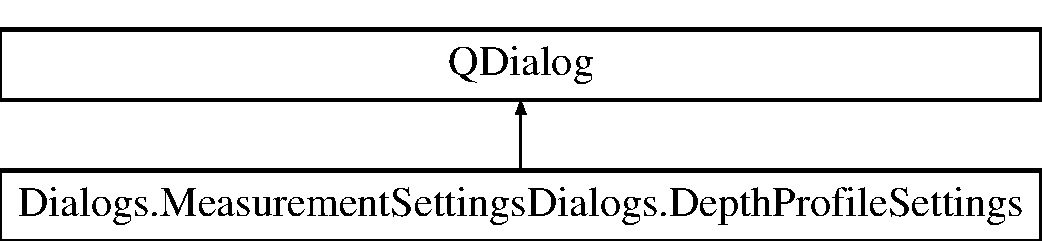
\includegraphics[height=2.000000cm]{classDialogs_1_1MeasurementSettingsDialogs_1_1DepthProfileSettings}
\end{center}
\end{figure}
\subsection*{Public Member Functions}
\begin{DoxyCompactItemize}
\item 
def \hyperlink{classDialogs_1_1MeasurementSettingsDialogs_1_1DepthProfileSettings_ad4116df69c127620657a3fde94b67178}{\-\_\-\-\_\-init\-\_\-\-\_\-}
\item 
def \hyperlink{classDialogs_1_1MeasurementSettingsDialogs_1_1DepthProfileSettings_aeddd8beb2aafb2cdb5d8dc3f70429a06}{update\-\_\-and\-\_\-close\-\_\-settings}
\end{DoxyCompactItemize}
\subsection*{Public Attributes}
\begin{DoxyCompactItemize}
\item 
\hypertarget{classDialogs_1_1MeasurementSettingsDialogs_1_1DepthProfileSettings_a100ec4396d2d91fe557dcb20509fe035}{{\bfseries default\-\_\-folder}}\label{classDialogs_1_1MeasurementSettingsDialogs_1_1DepthProfileSettings_a100ec4396d2d91fe557dcb20509fe035}

\item 
\hypertarget{classDialogs_1_1MeasurementSettingsDialogs_1_1DepthProfileSettings_ab268ebbac8d57442cdbf4a1206c2570b}{{\bfseries ui}}\label{classDialogs_1_1MeasurementSettingsDialogs_1_1DepthProfileSettings_ab268ebbac8d57442cdbf4a1206c2570b}

\item 
\hypertarget{classDialogs_1_1MeasurementSettingsDialogs_1_1DepthProfileSettings_a84b2167c49802bedf7bd67044ad68107}{{\bfseries project\-\_\-settings}}\label{classDialogs_1_1MeasurementSettingsDialogs_1_1DepthProfileSettings_a84b2167c49802bedf7bd67044ad68107}

\item 
\hypertarget{classDialogs_1_1MeasurementSettingsDialogs_1_1DepthProfileSettings_ad94dd1bc1478021b942e3c234a2917e0}{{\bfseries settings}}\label{classDialogs_1_1MeasurementSettingsDialogs_1_1DepthProfileSettings_ad94dd1bc1478021b942e3c234a2917e0}

\end{DoxyCompactItemize}


\subsection{Constructor \& Destructor Documentation}
\hypertarget{classDialogs_1_1MeasurementSettingsDialogs_1_1DepthProfileSettings_ad4116df69c127620657a3fde94b67178}{\index{Dialogs\-::\-Measurement\-Settings\-Dialogs\-::\-Depth\-Profile\-Settings@{Dialogs\-::\-Measurement\-Settings\-Dialogs\-::\-Depth\-Profile\-Settings}!\-\_\-\-\_\-init\-\_\-\-\_\-@{\-\_\-\-\_\-init\-\_\-\-\_\-}}
\index{\-\_\-\-\_\-init\-\_\-\-\_\-@{\-\_\-\-\_\-init\-\_\-\-\_\-}!Dialogs::MeasurementSettingsDialogs::DepthProfileSettings@{Dialogs\-::\-Measurement\-Settings\-Dialogs\-::\-Depth\-Profile\-Settings}}
\subsubsection[{\-\_\-\-\_\-init\-\_\-\-\_\-}]{\setlength{\rightskip}{0pt plus 5cm}def Dialogs.\-Measurement\-Settings\-Dialogs.\-Depth\-Profile\-Settings.\-\_\-\-\_\-init\-\_\-\-\_\- (
\begin{DoxyParamCaption}
\item[{}]{self, }
\item[{}]{measurement\-\_\-settings}
\end{DoxyParamCaption}
)}}\label{classDialogs_1_1MeasurementSettingsDialogs_1_1DepthProfileSettings_ad4116df69c127620657a3fde94b67178}
\begin{DoxyVerb}Constructor for the program

Args:
    measurement_settings:    
\end{DoxyVerb}
 

\subsection{Member Function Documentation}
\hypertarget{classDialogs_1_1MeasurementSettingsDialogs_1_1DepthProfileSettings_aeddd8beb2aafb2cdb5d8dc3f70429a06}{\index{Dialogs\-::\-Measurement\-Settings\-Dialogs\-::\-Depth\-Profile\-Settings@{Dialogs\-::\-Measurement\-Settings\-Dialogs\-::\-Depth\-Profile\-Settings}!update\-\_\-and\-\_\-close\-\_\-settings@{update\-\_\-and\-\_\-close\-\_\-settings}}
\index{update\-\_\-and\-\_\-close\-\_\-settings@{update\-\_\-and\-\_\-close\-\_\-settings}!Dialogs::MeasurementSettingsDialogs::DepthProfileSettings@{Dialogs\-::\-Measurement\-Settings\-Dialogs\-::\-Depth\-Profile\-Settings}}
\subsubsection[{update\-\_\-and\-\_\-close\-\_\-settings}]{\setlength{\rightskip}{0pt plus 5cm}def Dialogs.\-Measurement\-Settings\-Dialogs.\-Depth\-Profile\-Settings.\-update\-\_\-and\-\_\-close\-\_\-settings (
\begin{DoxyParamCaption}
\item[{}]{self}
\end{DoxyParamCaption}
)}}\label{classDialogs_1_1MeasurementSettingsDialogs_1_1DepthProfileSettings_aeddd8beb2aafb2cdb5d8dc3f70429a06}
\begin{DoxyVerb}Updates measuring settings values with the dialog's values and saves them to default ini file.
\end{DoxyVerb}
 

The documentation for this class was generated from the following file\-:\begin{DoxyCompactItemize}
\item 
Dialogs/Measurement\-Settings\-Dialogs.\-py\end{DoxyCompactItemize}

\hypertarget{classDialogs_1_1DepthProfileDialog_1_1DepthProfileWidget}{\section{Dialogs.\-Depth\-Profile\-Dialog.\-Depth\-Profile\-Widget Class Reference}
\label{classDialogs_1_1DepthProfileDialog_1_1DepthProfileWidget}\index{Dialogs.\-Depth\-Profile\-Dialog.\-Depth\-Profile\-Widget@{Dialogs.\-Depth\-Profile\-Dialog.\-Depth\-Profile\-Widget}}
}
Inheritance diagram for Dialogs.\-Depth\-Profile\-Dialog.\-Depth\-Profile\-Widget\-:\begin{figure}[H]
\begin{center}
\leavevmode
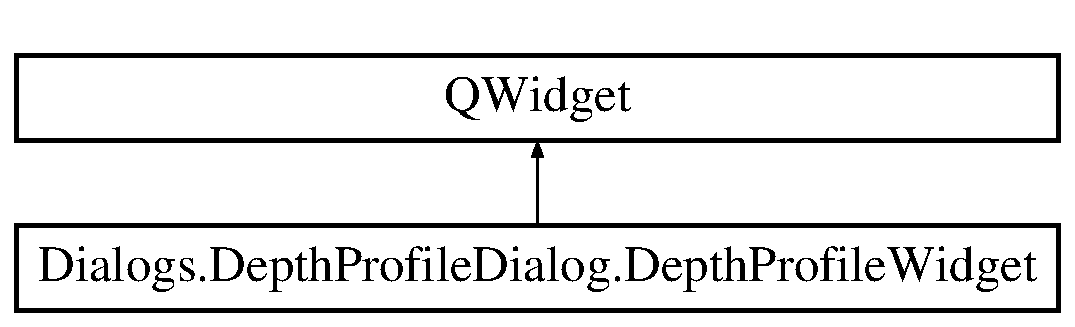
\includegraphics[height=2.000000cm]{classDialogs_1_1DepthProfileDialog_1_1DepthProfileWidget}
\end{center}
\end{figure}
\subsection*{Public Member Functions}
\begin{DoxyCompactItemize}
\item 
def \hyperlink{classDialogs_1_1DepthProfileDialog_1_1DepthProfileWidget_a6ce1e2fe9a2780398dd1e62f44245e31}{\-\_\-\-\_\-init\-\_\-\-\_\-}
\item 
def \hyperlink{classDialogs_1_1DepthProfileDialog_1_1DepthProfileWidget_ab8d159ad6d502f044900f2f50554e631}{delete}
\item 
def \hyperlink{classDialogs_1_1DepthProfileDialog_1_1DepthProfileWidget_afde62bd6a622e339b46de34dbe6e310f}{close\-Event}
\item 
def \hyperlink{classDialogs_1_1DepthProfileDialog_1_1DepthProfileWidget_a06713c36f62be4f15cdfe1e2baad39bf}{save\-\_\-to\-\_\-file}
\end{DoxyCompactItemize}
\subsection*{Public Attributes}
\begin{DoxyCompactItemize}
\item 
\hypertarget{classDialogs_1_1DepthProfileDialog_1_1DepthProfileWidget_a2ce1a2cecb250cb85590cd964d40f3ed}{{\bfseries parent}}\label{classDialogs_1_1DepthProfileDialog_1_1DepthProfileWidget_a2ce1a2cecb250cb85590cd964d40f3ed}

\item 
\hypertarget{classDialogs_1_1DepthProfileDialog_1_1DepthProfileWidget_ab27c1e45c9c99a0034172d9b4f87a9a9}{{\bfseries icon\-\_\-manager}}\label{classDialogs_1_1DepthProfileDialog_1_1DepthProfileWidget_ab27c1e45c9c99a0034172d9b4f87a9a9}

\item 
\hypertarget{classDialogs_1_1DepthProfileDialog_1_1DepthProfileWidget_a99b388eba8e3c405eb156b1704dfda2d}{{\bfseries measurement}}\label{classDialogs_1_1DepthProfileDialog_1_1DepthProfileWidget_a99b388eba8e3c405eb156b1704dfda2d}

\item 
\hypertarget{classDialogs_1_1DepthProfileDialog_1_1DepthProfileWidget_a53a8fea97aea9265b597638a690dee5f}{{\bfseries output\-\_\-dir}}\label{classDialogs_1_1DepthProfileDialog_1_1DepthProfileWidget_a53a8fea97aea9265b597638a690dee5f}

\item 
\hypertarget{classDialogs_1_1DepthProfileDialog_1_1DepthProfileWidget_a7e38ffd405b6643e7521230006fda168}{{\bfseries elements}}\label{classDialogs_1_1DepthProfileDialog_1_1DepthProfileWidget_a7e38ffd405b6643e7521230006fda168}

\item 
\hypertarget{classDialogs_1_1DepthProfileDialog_1_1DepthProfileWidget_abed68665550cebd6d6f9c55881f259f7}{{\bfseries x\-\_\-units}}\label{classDialogs_1_1DepthProfileDialog_1_1DepthProfileWidget_abed68665550cebd6d6f9c55881f259f7}

\item 
\hypertarget{classDialogs_1_1DepthProfileDialog_1_1DepthProfileWidget_a4caa4180c484caf2d299a22c44b85f00}{{\bfseries ui}}\label{classDialogs_1_1DepthProfileDialog_1_1DepthProfileWidget_a4caa4180c484caf2d299a22c44b85f00}

\item 
\hypertarget{classDialogs_1_1DepthProfileDialog_1_1DepthProfileWidget_a4051e29dc911df290e34832833d55f25}{{\bfseries matplotlib}}\label{classDialogs_1_1DepthProfileDialog_1_1DepthProfileWidget_a4051e29dc911df290e34832833d55f25}

\end{DoxyCompactItemize}
\subsection*{Static Public Attributes}
\begin{DoxyCompactItemize}
\item 
\hypertarget{classDialogs_1_1DepthProfileDialog_1_1DepthProfileWidget_ac519dfb8a1a94fc5444da09d10cad600}{string {\bfseries save\-\_\-file} = \char`\"{}widget\-\_\-depth\-\_\-profile.\-save\char`\"{}}\label{classDialogs_1_1DepthProfileDialog_1_1DepthProfileWidget_ac519dfb8a1a94fc5444da09d10cad600}

\end{DoxyCompactItemize}


\subsection{Detailed Description}
\begin{DoxyVerb}Depth Profile widget which is added to measurement tab.
\end{DoxyVerb}
 

\subsection{Constructor \& Destructor Documentation}
\hypertarget{classDialogs_1_1DepthProfileDialog_1_1DepthProfileWidget_a6ce1e2fe9a2780398dd1e62f44245e31}{\index{Dialogs\-::\-Depth\-Profile\-Dialog\-::\-Depth\-Profile\-Widget@{Dialogs\-::\-Depth\-Profile\-Dialog\-::\-Depth\-Profile\-Widget}!\-\_\-\-\_\-init\-\_\-\-\_\-@{\-\_\-\-\_\-init\-\_\-\-\_\-}}
\index{\-\_\-\-\_\-init\-\_\-\-\_\-@{\-\_\-\-\_\-init\-\_\-\-\_\-}!Dialogs::DepthProfileDialog::DepthProfileWidget@{Dialogs\-::\-Depth\-Profile\-Dialog\-::\-Depth\-Profile\-Widget}}
\subsubsection[{\-\_\-\-\_\-init\-\_\-\-\_\-}]{\setlength{\rightskip}{0pt plus 5cm}def Dialogs.\-Depth\-Profile\-Dialog.\-Depth\-Profile\-Widget.\-\_\-\-\_\-init\-\_\-\-\_\- (
\begin{DoxyParamCaption}
\item[{}]{self, }
\item[{}]{parent, }
\item[{}]{output\-\_\-dir, }
\item[{}]{use\-\_\-cuts, }
\item[{}]{elements, }
\item[{}]{x\-\_\-units, }
\item[{}]{line\-\_\-zero, }
\item[{}]{line\-\_\-scale, }
\item[{}]{systematic\-\_\-error}
\end{DoxyParamCaption}
)}}\label{classDialogs_1_1DepthProfileDialog_1_1DepthProfileWidget_a6ce1e2fe9a2780398dd1e62f44245e31}
\begin{DoxyVerb}Inits widget.

Args:
    parent: A MeasurementTabWidget.
    output_dir: A string representing directory in which the depth files 
        are located.
    use_cuts: A string list representing Cut files.
    elements: A list of Element objects that are used in depth profile.
    x_units: Units to be used for x-axis of depth profile.
    line_zero: A boolean representing if vertical line is drawn at zero.
    line_scale: A boolean representing if horizontal line is drawn at 
        the defined depth scale.
    systematic_error: A double representing systematic error.
\end{DoxyVerb}
 

\subsection{Member Function Documentation}
\hypertarget{classDialogs_1_1DepthProfileDialog_1_1DepthProfileWidget_afde62bd6a622e339b46de34dbe6e310f}{\index{Dialogs\-::\-Depth\-Profile\-Dialog\-::\-Depth\-Profile\-Widget@{Dialogs\-::\-Depth\-Profile\-Dialog\-::\-Depth\-Profile\-Widget}!close\-Event@{close\-Event}}
\index{close\-Event@{close\-Event}!Dialogs::DepthProfileDialog::DepthProfileWidget@{Dialogs\-::\-Depth\-Profile\-Dialog\-::\-Depth\-Profile\-Widget}}
\subsubsection[{close\-Event}]{\setlength{\rightskip}{0pt plus 5cm}def Dialogs.\-Depth\-Profile\-Dialog.\-Depth\-Profile\-Widget.\-close\-Event (
\begin{DoxyParamCaption}
\item[{}]{self, }
\item[{}]{evnt}
\end{DoxyParamCaption}
)}}\label{classDialogs_1_1DepthProfileDialog_1_1DepthProfileWidget_afde62bd6a622e339b46de34dbe6e310f}
\begin{DoxyVerb}Reimplemented method when closing widget.
\end{DoxyVerb}
 \hypertarget{classDialogs_1_1DepthProfileDialog_1_1DepthProfileWidget_ab8d159ad6d502f044900f2f50554e631}{\index{Dialogs\-::\-Depth\-Profile\-Dialog\-::\-Depth\-Profile\-Widget@{Dialogs\-::\-Depth\-Profile\-Dialog\-::\-Depth\-Profile\-Widget}!delete@{delete}}
\index{delete@{delete}!Dialogs::DepthProfileDialog::DepthProfileWidget@{Dialogs\-::\-Depth\-Profile\-Dialog\-::\-Depth\-Profile\-Widget}}
\subsubsection[{delete}]{\setlength{\rightskip}{0pt plus 5cm}def Dialogs.\-Depth\-Profile\-Dialog.\-Depth\-Profile\-Widget.\-delete (
\begin{DoxyParamCaption}
\item[{}]{self}
\end{DoxyParamCaption}
)}}\label{classDialogs_1_1DepthProfileDialog_1_1DepthProfileWidget_ab8d159ad6d502f044900f2f50554e631}
\begin{DoxyVerb}Delete variables and do clean up.
\end{DoxyVerb}
 \hypertarget{classDialogs_1_1DepthProfileDialog_1_1DepthProfileWidget_a06713c36f62be4f15cdfe1e2baad39bf}{\index{Dialogs\-::\-Depth\-Profile\-Dialog\-::\-Depth\-Profile\-Widget@{Dialogs\-::\-Depth\-Profile\-Dialog\-::\-Depth\-Profile\-Widget}!save\-\_\-to\-\_\-file@{save\-\_\-to\-\_\-file}}
\index{save\-\_\-to\-\_\-file@{save\-\_\-to\-\_\-file}!Dialogs::DepthProfileDialog::DepthProfileWidget@{Dialogs\-::\-Depth\-Profile\-Dialog\-::\-Depth\-Profile\-Widget}}
\subsubsection[{save\-\_\-to\-\_\-file}]{\setlength{\rightskip}{0pt plus 5cm}def Dialogs.\-Depth\-Profile\-Dialog.\-Depth\-Profile\-Widget.\-save\-\_\-to\-\_\-file (
\begin{DoxyParamCaption}
\item[{}]{self}
\end{DoxyParamCaption}
)}}\label{classDialogs_1_1DepthProfileDialog_1_1DepthProfileWidget_a06713c36f62be4f15cdfe1e2baad39bf}
\begin{DoxyVerb}Save object information to file.
\end{DoxyVerb}
 

The documentation for this class was generated from the following file\-:\begin{DoxyCompactItemize}
\item 
Dialogs/Depth\-Profile\-Dialog.\-py\end{DoxyCompactItemize}

\hypertarget{classModules_1_1Element_1_1Element}{\section{Modules.\-Element.\-Element Class Reference}
\label{classModules_1_1Element_1_1Element}\index{Modules.\-Element.\-Element@{Modules.\-Element.\-Element}}
}
\subsection*{Public Member Functions}
\begin{DoxyCompactItemize}
\item 
def \hyperlink{classModules_1_1Element_1_1Element_aaf833476ec5e1ea65586c59dfec00df9}{\-\_\-\-\_\-init\-\_\-\-\_\-}
\item 
def \hyperlink{classModules_1_1Element_1_1Element_a7a7a9209ae83aa96adb7a51cda42574f}{\-\_\-\-\_\-str\-\_\-\-\_\-}
\item 
def \hyperlink{classModules_1_1Element_1_1Element_aa966376c457405db42de5279c4c38128}{\-\_\-\-\_\-eq\-\_\-\-\_\-}
\item 
def \hyperlink{classModules_1_1Element_1_1Element_a903672dc2f6856bc0ac2ac5862f8b068}{get\-\_\-element\-\_\-and\-\_\-isotope}
\end{DoxyCompactItemize}
\subsection*{Public Attributes}
\begin{DoxyCompactItemize}
\item 
\hypertarget{classModules_1_1Element_1_1Element_ae0ed1337973bdfbf2e694123b524d86a}{{\bfseries name}}\label{classModules_1_1Element_1_1Element_ae0ed1337973bdfbf2e694123b524d86a}

\item 
\hypertarget{classModules_1_1Element_1_1Element_a36586f144787a88e5c6e3fc5c8ba94f4}{{\bfseries isotope}}\label{classModules_1_1Element_1_1Element_a36586f144787a88e5c6e3fc5c8ba94f4}

\end{DoxyCompactItemize}


\subsection{Constructor \& Destructor Documentation}
\hypertarget{classModules_1_1Element_1_1Element_aaf833476ec5e1ea65586c59dfec00df9}{\index{Modules\-::\-Element\-::\-Element@{Modules\-::\-Element\-::\-Element}!\-\_\-\-\_\-init\-\_\-\-\_\-@{\-\_\-\-\_\-init\-\_\-\-\_\-}}
\index{\-\_\-\-\_\-init\-\_\-\-\_\-@{\-\_\-\-\_\-init\-\_\-\-\_\-}!Modules::Element::Element@{Modules\-::\-Element\-::\-Element}}
\subsubsection[{\-\_\-\-\_\-init\-\_\-\-\_\-}]{\setlength{\rightskip}{0pt plus 5cm}def Modules.\-Element.\-Element.\-\_\-\-\_\-init\-\_\-\-\_\- (
\begin{DoxyParamCaption}
\item[{}]{self, }
\item[{}]{element = {\ttfamily \char`\"{}\char`\"{}}, }
\item[{}]{isotope = {\ttfamily None}}
\end{DoxyParamCaption}
)}}\label{classModules_1_1Element_1_1Element_aaf833476ec5e1ea65586c59dfec00df9}
\begin{DoxyVerb}Inits element class.        

>>> test_a = Element("1H")
>>> test_b = Element("H")
>>> test_c = Element("H", 1)
>>> test_d = Element("Ca", 40)
>>> test_e = Element("")
>>> test_f = Element("H1")
>>> print(test_a)
1H
>>> print(test_b)
H
>>> print(test_c)
1H
>>> print(test_d)
40Ca
>>> print(test_f) # Suppose we ignore numbers or whatever after element.
H
\end{DoxyVerb}
 

\subsection{Member Function Documentation}
\hypertarget{classModules_1_1Element_1_1Element_aa966376c457405db42de5279c4c38128}{\index{Modules\-::\-Element\-::\-Element@{Modules\-::\-Element\-::\-Element}!\-\_\-\-\_\-eq\-\_\-\-\_\-@{\-\_\-\-\_\-eq\-\_\-\-\_\-}}
\index{\-\_\-\-\_\-eq\-\_\-\-\_\-@{\-\_\-\-\_\-eq\-\_\-\-\_\-}!Modules::Element::Element@{Modules\-::\-Element\-::\-Element}}
\subsubsection[{\-\_\-\-\_\-eq\-\_\-\-\_\-}]{\setlength{\rightskip}{0pt plus 5cm}def Modules.\-Element.\-Element.\-\_\-\-\_\-eq\-\_\-\-\_\- (
\begin{DoxyParamCaption}
\item[{}]{self, }
\item[{}]{other}
\end{DoxyParamCaption}
)}}\label{classModules_1_1Element_1_1Element_aa966376c457405db42de5279c4c38128}
\begin{DoxyVerb}Compare object.
\end{DoxyVerb}
 \hypertarget{classModules_1_1Element_1_1Element_a7a7a9209ae83aa96adb7a51cda42574f}{\index{Modules\-::\-Element\-::\-Element@{Modules\-::\-Element\-::\-Element}!\-\_\-\-\_\-str\-\_\-\-\_\-@{\-\_\-\-\_\-str\-\_\-\-\_\-}}
\index{\-\_\-\-\_\-str\-\_\-\-\_\-@{\-\_\-\-\_\-str\-\_\-\-\_\-}!Modules::Element::Element@{Modules\-::\-Element\-::\-Element}}
\subsubsection[{\-\_\-\-\_\-str\-\_\-\-\_\-}]{\setlength{\rightskip}{0pt plus 5cm}def Modules.\-Element.\-Element.\-\_\-\-\_\-str\-\_\-\-\_\- (
\begin{DoxyParamCaption}
\item[{}]{self}
\end{DoxyParamCaption}
)}}\label{classModules_1_1Element_1_1Element_a7a7a9209ae83aa96adb7a51cda42574f}
\begin{DoxyVerb}Transform element into string.

Return:
    Returns element and its isotope in string format.
\end{DoxyVerb}
 \hypertarget{classModules_1_1Element_1_1Element_a903672dc2f6856bc0ac2ac5862f8b068}{\index{Modules\-::\-Element\-::\-Element@{Modules\-::\-Element\-::\-Element}!get\-\_\-element\-\_\-and\-\_\-isotope@{get\-\_\-element\-\_\-and\-\_\-isotope}}
\index{get\-\_\-element\-\_\-and\-\_\-isotope@{get\-\_\-element\-\_\-and\-\_\-isotope}!Modules::Element::Element@{Modules\-::\-Element\-::\-Element}}
\subsubsection[{get\-\_\-element\-\_\-and\-\_\-isotope}]{\setlength{\rightskip}{0pt plus 5cm}def Modules.\-Element.\-Element.\-get\-\_\-element\-\_\-and\-\_\-isotope (
\begin{DoxyParamCaption}
\item[{}]{self}
\end{DoxyParamCaption}
)}}\label{classModules_1_1Element_1_1Element_a903672dc2f6856bc0ac2ac5862f8b068}
\begin{DoxyVerb}Get Element's name and isotope.

Return:
    Returns element's name (string) and its isotope (class object).
\end{DoxyVerb}
 

The documentation for this class was generated from the following file\-:\begin{DoxyCompactItemize}
\item 
Modules/Element.\-py\end{DoxyCompactItemize}

\hypertarget{classModules_1_1ElementLosses_1_1ElementLosses}{\section{Modules.\-Element\-Losses.\-Element\-Losses Class Reference}
\label{classModules_1_1ElementLosses_1_1ElementLosses}\index{Modules.\-Element\-Losses.\-Element\-Losses@{Modules.\-Element\-Losses.\-Element\-Losses}}
}
\subsection*{Public Member Functions}
\begin{DoxyCompactItemize}
\item 
def \hyperlink{classModules_1_1ElementLosses_1_1ElementLosses_aa19d25723c97a424378699fcaba8edce}{\-\_\-\-\_\-init\-\_\-\-\_\-}
\item 
def \hyperlink{classModules_1_1ElementLosses_1_1ElementLosses_afdf9c1017acdecea3d66b02264849a6c}{count\-\_\-element\-\_\-cuts}
\item 
def \hyperlink{classModules_1_1ElementLosses_1_1ElementLosses_a5752d0dfbab2168077fe962bb47564e8}{save\-\_\-splits}
\end{DoxyCompactItemize}
\subsection*{Public Attributes}
\begin{DoxyCompactItemize}
\item 
\hypertarget{classModules_1_1ElementLosses_1_1ElementLosses_a44baf5bdb5fae4b24f824610ee074efe}{{\bfseries directory\-\_\-cuts}}\label{classModules_1_1ElementLosses_1_1ElementLosses_a44baf5bdb5fae4b24f824610ee074efe}

\item 
\hypertarget{classModules_1_1ElementLosses_1_1ElementLosses_a1170dc18667785a830f0f2807aed9f98}{{\bfseries directory\-\_\-elemloss}}\label{classModules_1_1ElementLosses_1_1ElementLosses_a1170dc18667785a830f0f2807aed9f98}

\item 
\hypertarget{classModules_1_1ElementLosses_1_1ElementLosses_a28bae738639f3f09c6b8cc597c65ca32}{{\bfseries partition\-\_\-count}}\label{classModules_1_1ElementLosses_1_1ElementLosses_a28bae738639f3f09c6b8cc597c65ca32}

\item 
\hypertarget{classModules_1_1ElementLosses_1_1ElementLosses_a09f801e73a7118d0091ce539734a70d7}{{\bfseries checked\-\_\-cuts}}\label{classModules_1_1ElementLosses_1_1ElementLosses_a09f801e73a7118d0091ce539734a70d7}

\item 
\hypertarget{classModules_1_1ElementLosses_1_1ElementLosses_a832b370bdd2ac74180389c3ba9bd4cb6}{{\bfseries progress\-\_\-bar}}\label{classModules_1_1ElementLosses_1_1ElementLosses_a832b370bdd2ac74180389c3ba9bd4cb6}

\item 
\hypertarget{classModules_1_1ElementLosses_1_1ElementLosses_a8efdcf2bb38abcefaa510d5a4c17197b}{{\bfseries reference\-\_\-cut\-\_\-file}}\label{classModules_1_1ElementLosses_1_1ElementLosses_a8efdcf2bb38abcefaa510d5a4c17197b}

\item 
\hypertarget{classModules_1_1ElementLosses_1_1ElementLosses_ae9cdb055926a4c6bf78d314e72c70ad6}{{\bfseries reference\-\_\-key}}\label{classModules_1_1ElementLosses_1_1ElementLosses_ae9cdb055926a4c6bf78d314e72c70ad6}

\item 
\hypertarget{classModules_1_1ElementLosses_1_1ElementLosses_af849a17430c56e57ee35df40ef3b62e8}{{\bfseries cut\-\_\-splits}}\label{classModules_1_1ElementLosses_1_1ElementLosses_af849a17430c56e57ee35df40ef3b62e8}

\item 
\hypertarget{classModules_1_1ElementLosses_1_1ElementLosses_a61e4e32edba50f979cbea62749a455ef}{{\bfseries reference\-\_\-cut}}\label{classModules_1_1ElementLosses_1_1ElementLosses_a61e4e32edba50f979cbea62749a455ef}

\end{DoxyCompactItemize}


\subsection{Detailed Description}
\begin{DoxyVerb}Element Losses class.
\end{DoxyVerb}
 

\subsection{Constructor \& Destructor Documentation}
\hypertarget{classModules_1_1ElementLosses_1_1ElementLosses_aa19d25723c97a424378699fcaba8edce}{\index{Modules\-::\-Element\-Losses\-::\-Element\-Losses@{Modules\-::\-Element\-Losses\-::\-Element\-Losses}!\-\_\-\-\_\-init\-\_\-\-\_\-@{\-\_\-\-\_\-init\-\_\-\-\_\-}}
\index{\-\_\-\-\_\-init\-\_\-\-\_\-@{\-\_\-\-\_\-init\-\_\-\-\_\-}!Modules::ElementLosses::ElementLosses@{Modules\-::\-Element\-Losses\-::\-Element\-Losses}}
\subsubsection[{\-\_\-\-\_\-init\-\_\-\-\_\-}]{\setlength{\rightskip}{0pt plus 5cm}def Modules.\-Element\-Losses.\-Element\-Losses.\-\_\-\-\_\-init\-\_\-\-\_\- (
\begin{DoxyParamCaption}
\item[{}]{self, }
\item[{}]{directory\-\_\-cuts, }
\item[{}]{directory\-\_\-elemloss, }
\item[{}]{reference\-\_\-cut\-\_\-file, }
\item[{}]{checked\-\_\-cuts, }
\item[{}]{partition\-\_\-count, }
\item[{}]{progress\-\_\-bar = {\ttfamily {\bf Null}()}}
\end{DoxyParamCaption}
)}}\label{classModules_1_1ElementLosses_1_1ElementLosses_aa19d25723c97a424378699fcaba8edce}
\begin{DoxyVerb}Inits Element Losses class.

Args:
    directory_cuts: String representing cut file directory.
    directory_elemloss: String representing elemental losses directory.
    reference_cut_file: String representing reference cut file.
    checked_cuts: String list of cut files to be graphed.
    partition_count: Integer representing split count.
    progress_bar: QtWidgets.QProgressBar or Null() if not given.
\end{DoxyVerb}
 

\subsection{Member Function Documentation}
\hypertarget{classModules_1_1ElementLosses_1_1ElementLosses_afdf9c1017acdecea3d66b02264849a6c}{\index{Modules\-::\-Element\-Losses\-::\-Element\-Losses@{Modules\-::\-Element\-Losses\-::\-Element\-Losses}!count\-\_\-element\-\_\-cuts@{count\-\_\-element\-\_\-cuts}}
\index{count\-\_\-element\-\_\-cuts@{count\-\_\-element\-\_\-cuts}!Modules::ElementLosses::ElementLosses@{Modules\-::\-Element\-Losses\-::\-Element\-Losses}}
\subsubsection[{count\-\_\-element\-\_\-cuts}]{\setlength{\rightskip}{0pt plus 5cm}def Modules.\-Element\-Losses.\-Element\-Losses.\-count\-\_\-element\-\_\-cuts (
\begin{DoxyParamCaption}
\item[{}]{self, }
\item[{}]{save\-\_\-splits = {\ttfamily False}}
\end{DoxyParamCaption}
)}}\label{classModules_1_1ElementLosses_1_1ElementLosses_afdf9c1017acdecea3d66b02264849a6c}
\begin{DoxyVerb}Count data points in splits based on reference file.

Args:
    save_splits: Boolean representing whether to save element losses splits.

Return:
    Returns dictionary of elements and their counts within splits.
\end{DoxyVerb}
 \hypertarget{classModules_1_1ElementLosses_1_1ElementLosses_a5752d0dfbab2168077fe962bb47564e8}{\index{Modules\-::\-Element\-Losses\-::\-Element\-Losses@{Modules\-::\-Element\-Losses\-::\-Element\-Losses}!save\-\_\-splits@{save\-\_\-splits}}
\index{save\-\_\-splits@{save\-\_\-splits}!Modules::ElementLosses::ElementLosses@{Modules\-::\-Element\-Losses\-::\-Element\-Losses}}
\subsubsection[{save\-\_\-splits}]{\setlength{\rightskip}{0pt plus 5cm}def Modules.\-Element\-Losses.\-Element\-Losses.\-save\-\_\-splits (
\begin{DoxyParamCaption}
\item[{}]{self}
\end{DoxyParamCaption}
)}}\label{classModules_1_1ElementLosses_1_1ElementLosses_a5752d0dfbab2168077fe962bb47564e8}
\begin{DoxyVerb}Save element splits as new cut files.
\end{DoxyVerb}
 

The documentation for this class was generated from the following file\-:\begin{DoxyCompactItemize}
\item 
Modules/Element\-Losses.\-py\end{DoxyCompactItemize}

\hypertarget{classDialogs_1_1ElementLossesDialog_1_1ElementLossesDialog}{\section{Dialogs.\-Element\-Losses\-Dialog.\-Element\-Losses\-Dialog Class Reference}
\label{classDialogs_1_1ElementLossesDialog_1_1ElementLossesDialog}\index{Dialogs.\-Element\-Losses\-Dialog.\-Element\-Losses\-Dialog@{Dialogs.\-Element\-Losses\-Dialog.\-Element\-Losses\-Dialog}}
}
Inheritance diagram for Dialogs.\-Element\-Losses\-Dialog.\-Element\-Losses\-Dialog\-:\begin{figure}[H]
\begin{center}
\leavevmode
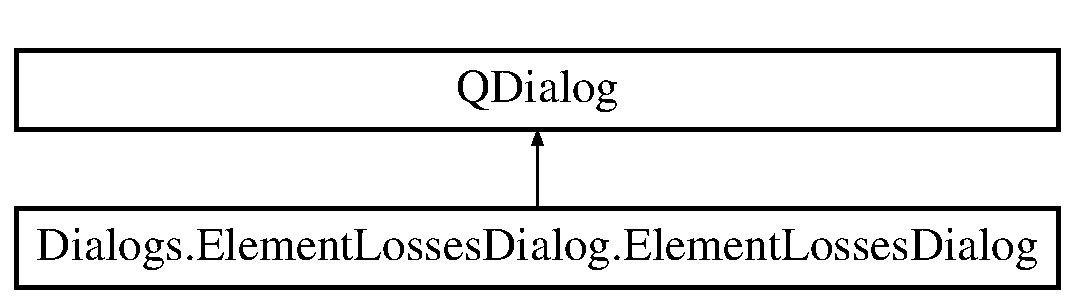
\includegraphics[height=2.000000cm]{classDialogs_1_1ElementLossesDialog_1_1ElementLossesDialog}
\end{center}
\end{figure}
\subsection*{Public Member Functions}
\begin{DoxyCompactItemize}
\item 
def \hyperlink{classDialogs_1_1ElementLossesDialog_1_1ElementLossesDialog_a6afdd9e38dff7e080a49eadd15e9d8c1}{\-\_\-\-\_\-init\-\_\-\-\_\-}
\end{DoxyCompactItemize}
\subsection*{Public Attributes}
\begin{DoxyCompactItemize}
\item 
\hypertarget{classDialogs_1_1ElementLossesDialog_1_1ElementLossesDialog_a6846ba3ab79e357c43602b2072490c01}{{\bfseries parent}}\label{classDialogs_1_1ElementLossesDialog_1_1ElementLossesDialog_a6846ba3ab79e357c43602b2072490c01}

\item 
\hypertarget{classDialogs_1_1ElementLossesDialog_1_1ElementLossesDialog_a5b73706c3d315d32f3db31d376814c6e}{{\bfseries cuts}}\label{classDialogs_1_1ElementLossesDialog_1_1ElementLossesDialog_a5b73706c3d315d32f3db31d376814c6e}

\item 
\hypertarget{classDialogs_1_1ElementLossesDialog_1_1ElementLossesDialog_a9a6774d19bd8b3dd1133d45f963c8a5d}{{\bfseries ui}}\label{classDialogs_1_1ElementLossesDialog_1_1ElementLossesDialog_a9a6774d19bd8b3dd1133d45f963c8a5d}

\end{DoxyCompactItemize}
\subsection*{Static Public Attributes}
\begin{DoxyCompactItemize}
\item 
\hypertarget{classDialogs_1_1ElementLossesDialog_1_1ElementLossesDialog_ad7a3b992570ed3b04ea9548c97ceff21}{dictionary {\bfseries checked\-\_\-cuts} = \{\}}\label{classDialogs_1_1ElementLossesDialog_1_1ElementLossesDialog_ad7a3b992570ed3b04ea9548c97ceff21}

\item 
\hypertarget{classDialogs_1_1ElementLossesDialog_1_1ElementLossesDialog_a4fa302c0f2ef47dab85f41bca5732e69}{dictionary {\bfseries reference\-\_\-cut} = \{\}}\label{classDialogs_1_1ElementLossesDialog_1_1ElementLossesDialog_a4fa302c0f2ef47dab85f41bca5732e69}

\item 
\hypertarget{classDialogs_1_1ElementLossesDialog_1_1ElementLossesDialog_a36fae53a5aca36a1e3d3e276969c8e3c}{int {\bfseries split\-\_\-count} = 10}\label{classDialogs_1_1ElementLossesDialog_1_1ElementLossesDialog_a36fae53a5aca36a1e3d3e276969c8e3c}

\item 
\hypertarget{classDialogs_1_1ElementLossesDialog_1_1ElementLossesDialog_add52a493975a9d085b496f2580e1228e}{int {\bfseries y\-\_\-scale} = 1}\label{classDialogs_1_1ElementLossesDialog_1_1ElementLossesDialog_add52a493975a9d085b496f2580e1228e}

\end{DoxyCompactItemize}


\subsection{Detailed Description}
\begin{DoxyVerb}Class to handle element losses dialogs.
\end{DoxyVerb}
 

\subsection{Constructor \& Destructor Documentation}
\hypertarget{classDialogs_1_1ElementLossesDialog_1_1ElementLossesDialog_a6afdd9e38dff7e080a49eadd15e9d8c1}{\index{Dialogs\-::\-Element\-Losses\-Dialog\-::\-Element\-Losses\-Dialog@{Dialogs\-::\-Element\-Losses\-Dialog\-::\-Element\-Losses\-Dialog}!\-\_\-\-\_\-init\-\_\-\-\_\-@{\-\_\-\-\_\-init\-\_\-\-\_\-}}
\index{\-\_\-\-\_\-init\-\_\-\-\_\-@{\-\_\-\-\_\-init\-\_\-\-\_\-}!Dialogs::ElementLossesDialog::ElementLossesDialog@{Dialogs\-::\-Element\-Losses\-Dialog\-::\-Element\-Losses\-Dialog}}
\subsubsection[{\-\_\-\-\_\-init\-\_\-\-\_\-}]{\setlength{\rightskip}{0pt plus 5cm}def Dialogs.\-Element\-Losses\-Dialog.\-Element\-Losses\-Dialog.\-\_\-\-\_\-init\-\_\-\-\_\- (
\begin{DoxyParamCaption}
\item[{}]{self, }
\item[{}]{parent}
\end{DoxyParamCaption}
)}}\label{classDialogs_1_1ElementLossesDialog_1_1ElementLossesDialog_a6afdd9e38dff7e080a49eadd15e9d8c1}
\begin{DoxyVerb}Inits element losses class.

 Args:
    parent: MeasurementTabWidget
\end{DoxyVerb}
 

The documentation for this class was generated from the following file\-:\begin{DoxyCompactItemize}
\item 
Dialogs/Element\-Losses\-Dialog.\-py\end{DoxyCompactItemize}

\hypertarget{classModules_1_1ElementLosses_1_1ElementLossesSplitHolder}{\section{Modules.\-Element\-Losses.\-Element\-Losses\-Split\-Holder Class Reference}
\label{classModules_1_1ElementLosses_1_1ElementLossesSplitHolder}\index{Modules.\-Element\-Losses.\-Element\-Losses\-Split\-Holder@{Modules.\-Element\-Losses.\-Element\-Losses\-Split\-Holder}}
}
\subsection*{Public Member Functions}
\begin{DoxyCompactItemize}
\item 
def \hyperlink{classModules_1_1ElementLosses_1_1ElementLossesSplitHolder_a10dece857ae109f5dd54e0c3b174d494}{\-\_\-\-\_\-init\-\_\-\-\_\-}
\item 
def \hyperlink{classModules_1_1ElementLosses_1_1ElementLossesSplitHolder_ad696a678a536b6b16a85e6a181df0853}{count}
\item 
def \hyperlink{classModules_1_1ElementLosses_1_1ElementLossesSplitHolder_a996005ee923a5c517529606092a0c069}{get\-\_\-keys}
\item 
def \hyperlink{classModules_1_1ElementLosses_1_1ElementLossesSplitHolder_ace7a9dfee09f35d6b5a73abe0a854b24}{get\-\_\-cut}
\item 
def \hyperlink{classModules_1_1ElementLosses_1_1ElementLossesSplitHolder_a6c07df9dce43b4dc06836d1643147d6d}{get\-\_\-splits}
\item 
def \hyperlink{classModules_1_1ElementLosses_1_1ElementLossesSplitHolder_af8c98d13c855b700f67d278ed6813cf3}{add\-\_\-splits}
\end{DoxyCompactItemize}


\subsection{Detailed Description}
\begin{DoxyVerb}Element Losses Split Holder class to hold information of cuts' splits.
\end{DoxyVerb}
 

\subsection{Constructor \& Destructor Documentation}
\hypertarget{classModules_1_1ElementLosses_1_1ElementLossesSplitHolder_a10dece857ae109f5dd54e0c3b174d494}{\index{Modules\-::\-Element\-Losses\-::\-Element\-Losses\-Split\-Holder@{Modules\-::\-Element\-Losses\-::\-Element\-Losses\-Split\-Holder}!\-\_\-\-\_\-init\-\_\-\-\_\-@{\-\_\-\-\_\-init\-\_\-\-\_\-}}
\index{\-\_\-\-\_\-init\-\_\-\-\_\-@{\-\_\-\-\_\-init\-\_\-\-\_\-}!Modules::ElementLosses::ElementLossesSplitHolder@{Modules\-::\-Element\-Losses\-::\-Element\-Losses\-Split\-Holder}}
\subsubsection[{\-\_\-\-\_\-init\-\_\-\-\_\-}]{\setlength{\rightskip}{0pt plus 5cm}def Modules.\-Element\-Losses.\-Element\-Losses\-Split\-Holder.\-\_\-\-\_\-init\-\_\-\-\_\- (
\begin{DoxyParamCaption}
\item[{}]{self}
\end{DoxyParamCaption}
)}}\label{classModules_1_1ElementLosses_1_1ElementLossesSplitHolder_a10dece857ae109f5dd54e0c3b174d494}
\begin{DoxyVerb}Inits the class
\end{DoxyVerb}
 

\subsection{Member Function Documentation}
\hypertarget{classModules_1_1ElementLosses_1_1ElementLossesSplitHolder_af8c98d13c855b700f67d278ed6813cf3}{\index{Modules\-::\-Element\-Losses\-::\-Element\-Losses\-Split\-Holder@{Modules\-::\-Element\-Losses\-::\-Element\-Losses\-Split\-Holder}!add\-\_\-splits@{add\-\_\-splits}}
\index{add\-\_\-splits@{add\-\_\-splits}!Modules::ElementLosses::ElementLossesSplitHolder@{Modules\-::\-Element\-Losses\-::\-Element\-Losses\-Split\-Holder}}
\subsubsection[{add\-\_\-splits}]{\setlength{\rightskip}{0pt plus 5cm}def Modules.\-Element\-Losses.\-Element\-Losses\-Split\-Holder.\-add\-\_\-splits (
\begin{DoxyParamCaption}
\item[{}]{self, }
\item[{}]{key, }
\item[{}]{cut, }
\item[{}]{splits}
\end{DoxyParamCaption}
)}}\label{classModules_1_1ElementLosses_1_1ElementLossesSplitHolder_af8c98d13c855b700f67d278ed6813cf3}
\begin{DoxyVerb}Add splits to a cut file
\end{DoxyVerb}
 \hypertarget{classModules_1_1ElementLosses_1_1ElementLossesSplitHolder_ad696a678a536b6b16a85e6a181df0853}{\index{Modules\-::\-Element\-Losses\-::\-Element\-Losses\-Split\-Holder@{Modules\-::\-Element\-Losses\-::\-Element\-Losses\-Split\-Holder}!count@{count}}
\index{count@{count}!Modules::ElementLosses::ElementLossesSplitHolder@{Modules\-::\-Element\-Losses\-::\-Element\-Losses\-Split\-Holder}}
\subsubsection[{count}]{\setlength{\rightskip}{0pt plus 5cm}def Modules.\-Element\-Losses.\-Element\-Losses\-Split\-Holder.\-count (
\begin{DoxyParamCaption}
\item[{}]{self}
\end{DoxyParamCaption}
)}}\label{classModules_1_1ElementLosses_1_1ElementLossesSplitHolder_ad696a678a536b6b16a85e6a181df0853}
\begin{DoxyVerb}Get count of splits.

Return:
    Returns count of cut files splitted.
\end{DoxyVerb}
 \hypertarget{classModules_1_1ElementLosses_1_1ElementLossesSplitHolder_ace7a9dfee09f35d6b5a73abe0a854b24}{\index{Modules\-::\-Element\-Losses\-::\-Element\-Losses\-Split\-Holder@{Modules\-::\-Element\-Losses\-::\-Element\-Losses\-Split\-Holder}!get\-\_\-cut@{get\-\_\-cut}}
\index{get\-\_\-cut@{get\-\_\-cut}!Modules::ElementLosses::ElementLossesSplitHolder@{Modules\-::\-Element\-Losses\-::\-Element\-Losses\-Split\-Holder}}
\subsubsection[{get\-\_\-cut}]{\setlength{\rightskip}{0pt plus 5cm}def Modules.\-Element\-Losses.\-Element\-Losses\-Split\-Holder.\-get\-\_\-cut (
\begin{DoxyParamCaption}
\item[{}]{self, }
\item[{}]{key}
\end{DoxyParamCaption}
)}}\label{classModules_1_1ElementLosses_1_1ElementLossesSplitHolder_ace7a9dfee09f35d6b5a73abe0a854b24}
\begin{DoxyVerb}Get cut file used to make splits.
\end{DoxyVerb}
 \hypertarget{classModules_1_1ElementLosses_1_1ElementLossesSplitHolder_a996005ee923a5c517529606092a0c069}{\index{Modules\-::\-Element\-Losses\-::\-Element\-Losses\-Split\-Holder@{Modules\-::\-Element\-Losses\-::\-Element\-Losses\-Split\-Holder}!get\-\_\-keys@{get\-\_\-keys}}
\index{get\-\_\-keys@{get\-\_\-keys}!Modules::ElementLosses::ElementLossesSplitHolder@{Modules\-::\-Element\-Losses\-::\-Element\-Losses\-Split\-Holder}}
\subsubsection[{get\-\_\-keys}]{\setlength{\rightskip}{0pt plus 5cm}def Modules.\-Element\-Losses.\-Element\-Losses\-Split\-Holder.\-get\-\_\-keys (
\begin{DoxyParamCaption}
\item[{}]{self}
\end{DoxyParamCaption}
)}}\label{classModules_1_1ElementLosses_1_1ElementLossesSplitHolder_a996005ee923a5c517529606092a0c069}
\begin{DoxyVerb}Get keys of splits.

Return:
    Returns all keys that are currently used.
\end{DoxyVerb}
 \hypertarget{classModules_1_1ElementLosses_1_1ElementLossesSplitHolder_a6c07df9dce43b4dc06836d1643147d6d}{\index{Modules\-::\-Element\-Losses\-::\-Element\-Losses\-Split\-Holder@{Modules\-::\-Element\-Losses\-::\-Element\-Losses\-Split\-Holder}!get\-\_\-splits@{get\-\_\-splits}}
\index{get\-\_\-splits@{get\-\_\-splits}!Modules::ElementLosses::ElementLossesSplitHolder@{Modules\-::\-Element\-Losses\-::\-Element\-Losses\-Split\-Holder}}
\subsubsection[{get\-\_\-splits}]{\setlength{\rightskip}{0pt plus 5cm}def Modules.\-Element\-Losses.\-Element\-Losses\-Split\-Holder.\-get\-\_\-splits (
\begin{DoxyParamCaption}
\item[{}]{self, }
\item[{}]{key}
\end{DoxyParamCaption}
)}}\label{classModules_1_1ElementLosses_1_1ElementLossesSplitHolder_a6c07df9dce43b4dc06836d1643147d6d}
\begin{DoxyVerb}Get splits of a cut file.
\end{DoxyVerb}
 

The documentation for this class was generated from the following file\-:\begin{DoxyCompactItemize}
\item 
Modules/Element\-Losses.\-py\end{DoxyCompactItemize}

\hypertarget{classDialogs_1_1ElementLossesDialog_1_1ElementLossesWidget}{\section{Dialogs.\-Element\-Losses\-Dialog.\-Element\-Losses\-Widget Class Reference}
\label{classDialogs_1_1ElementLossesDialog_1_1ElementLossesWidget}\index{Dialogs.\-Element\-Losses\-Dialog.\-Element\-Losses\-Widget@{Dialogs.\-Element\-Losses\-Dialog.\-Element\-Losses\-Widget}}
}
Inheritance diagram for Dialogs.\-Element\-Losses\-Dialog.\-Element\-Losses\-Widget\-:\begin{figure}[H]
\begin{center}
\leavevmode
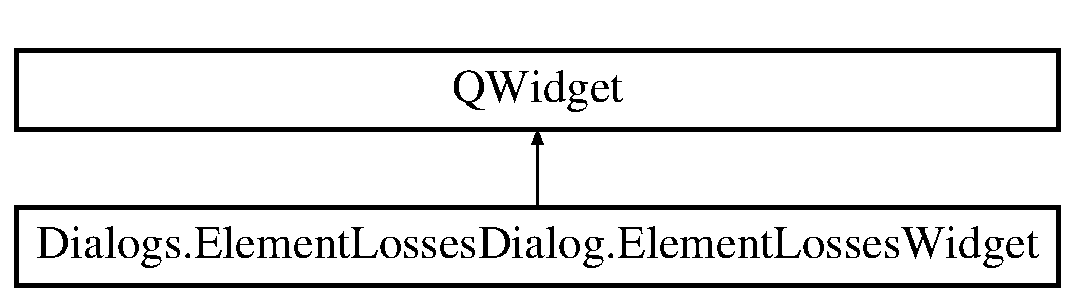
\includegraphics[height=2.000000cm]{classDialogs_1_1ElementLossesDialog_1_1ElementLossesWidget}
\end{center}
\end{figure}
\subsection*{Public Member Functions}
\begin{DoxyCompactItemize}
\item 
def \hyperlink{classDialogs_1_1ElementLossesDialog_1_1ElementLossesWidget_aa500c40b6c7b1d00780020c25489e0b2}{\-\_\-\-\_\-init\-\_\-\-\_\-}
\item 
def \hyperlink{classDialogs_1_1ElementLossesDialog_1_1ElementLossesWidget_a22fbeb57e6d1a772d76b273e5bcfa9a3}{delete}
\item 
def \hyperlink{classDialogs_1_1ElementLossesDialog_1_1ElementLossesWidget_af1506f3e49151f8ef37a536cee67a949}{close\-Event}
\item 
def \hyperlink{classDialogs_1_1ElementLossesDialog_1_1ElementLossesWidget_ac5f515fde2d5241d46c75f58dc32d103}{save\-\_\-to\-\_\-file}
\end{DoxyCompactItemize}
\subsection*{Public Attributes}
\begin{DoxyCompactItemize}
\item 
\hypertarget{classDialogs_1_1ElementLossesDialog_1_1ElementLossesWidget_a4c92e16dd5fc446ff04e463e486d786e}{{\bfseries parent}}\label{classDialogs_1_1ElementLossesDialog_1_1ElementLossesWidget_a4c92e16dd5fc446ff04e463e486d786e}

\item 
\hypertarget{classDialogs_1_1ElementLossesDialog_1_1ElementLossesWidget_ad22d757bb6cf31ad997800e10494f07e}{{\bfseries icon\-\_\-manager}}\label{classDialogs_1_1ElementLossesDialog_1_1ElementLossesWidget_ad22d757bb6cf31ad997800e10494f07e}

\item 
\hypertarget{classDialogs_1_1ElementLossesDialog_1_1ElementLossesWidget_a9e6fe553f32c7b7dbd3d8c0fef1f13fc}{{\bfseries measurement}}\label{classDialogs_1_1ElementLossesDialog_1_1ElementLossesWidget_a9e6fe553f32c7b7dbd3d8c0fef1f13fc}

\item 
\hypertarget{classDialogs_1_1ElementLossesDialog_1_1ElementLossesWidget_aba748b0fc9a987021be60a10839b7144}{{\bfseries reference\-\_\-cut\-\_\-file}}\label{classDialogs_1_1ElementLossesDialog_1_1ElementLossesWidget_aba748b0fc9a987021be60a10839b7144}

\item 
\hypertarget{classDialogs_1_1ElementLossesDialog_1_1ElementLossesWidget_a1585e037b7c18e03711ad826ea15342c}{{\bfseries checked\-\_\-cuts}}\label{classDialogs_1_1ElementLossesDialog_1_1ElementLossesWidget_a1585e037b7c18e03711ad826ea15342c}

\item 
\hypertarget{classDialogs_1_1ElementLossesDialog_1_1ElementLossesWidget_acaf966a5bc1e6be1f6979e98648de5ac}{{\bfseries partition\-\_\-count}}\label{classDialogs_1_1ElementLossesDialog_1_1ElementLossesWidget_acaf966a5bc1e6be1f6979e98648de5ac}

\item 
\hypertarget{classDialogs_1_1ElementLossesDialog_1_1ElementLossesWidget_ade0b6574747257bae3813008be218b1f}{{\bfseries y\-\_\-scale}}\label{classDialogs_1_1ElementLossesDialog_1_1ElementLossesWidget_ade0b6574747257bae3813008be218b1f}

\item 
\hypertarget{classDialogs_1_1ElementLossesDialog_1_1ElementLossesWidget_a900fa3f798aa83d264f97fb752f6824b}{{\bfseries progress\-\_\-bar}}\label{classDialogs_1_1ElementLossesDialog_1_1ElementLossesWidget_a900fa3f798aa83d264f97fb752f6824b}

\item 
\hypertarget{classDialogs_1_1ElementLossesDialog_1_1ElementLossesWidget_acd9a2370199adf25936817216fdc6f0d}{{\bfseries ui}}\label{classDialogs_1_1ElementLossesDialog_1_1ElementLossesWidget_acd9a2370199adf25936817216fdc6f0d}

\item 
\hypertarget{classDialogs_1_1ElementLossesDialog_1_1ElementLossesWidget_a3005579119e7ae7bbdb4617e0fc85ed9}{{\bfseries losses}}\label{classDialogs_1_1ElementLossesDialog_1_1ElementLossesWidget_a3005579119e7ae7bbdb4617e0fc85ed9}

\item 
\hypertarget{classDialogs_1_1ElementLossesDialog_1_1ElementLossesWidget_af40daea8f02908f07ae7956cd81e2fe2}{{\bfseries split\-\_\-counts}}\label{classDialogs_1_1ElementLossesDialog_1_1ElementLossesWidget_af40daea8f02908f07ae7956cd81e2fe2}

\item 
\hypertarget{classDialogs_1_1ElementLossesDialog_1_1ElementLossesWidget_aac2977387cef7e5be90e8eacc43a234c}{{\bfseries matplotlib}}\label{classDialogs_1_1ElementLossesDialog_1_1ElementLossesWidget_aac2977387cef7e5be90e8eacc43a234c}

\end{DoxyCompactItemize}
\subsection*{Static Public Attributes}
\begin{DoxyCompactItemize}
\item 
\hypertarget{classDialogs_1_1ElementLossesDialog_1_1ElementLossesWidget_ac90fe6871133f42b069e86f9c40dee2d}{string {\bfseries save\-\_\-file} = \char`\"{}widget\-\_\-elemental\-\_\-losses.\-save\char`\"{}}\label{classDialogs_1_1ElementLossesDialog_1_1ElementLossesWidget_ac90fe6871133f42b069e86f9c40dee2d}

\end{DoxyCompactItemize}


\subsection{Detailed Description}
\begin{DoxyVerb}Element losses widget which is added to measurement tab.
\end{DoxyVerb}
 

\subsection{Constructor \& Destructor Documentation}
\hypertarget{classDialogs_1_1ElementLossesDialog_1_1ElementLossesWidget_aa500c40b6c7b1d00780020c25489e0b2}{\index{Dialogs\-::\-Element\-Losses\-Dialog\-::\-Element\-Losses\-Widget@{Dialogs\-::\-Element\-Losses\-Dialog\-::\-Element\-Losses\-Widget}!\-\_\-\-\_\-init\-\_\-\-\_\-@{\-\_\-\-\_\-init\-\_\-\-\_\-}}
\index{\-\_\-\-\_\-init\-\_\-\-\_\-@{\-\_\-\-\_\-init\-\_\-\-\_\-}!Dialogs::ElementLossesDialog::ElementLossesWidget@{Dialogs\-::\-Element\-Losses\-Dialog\-::\-Element\-Losses\-Widget}}
\subsubsection[{\-\_\-\-\_\-init\-\_\-\-\_\-}]{\setlength{\rightskip}{0pt plus 5cm}def Dialogs.\-Element\-Losses\-Dialog.\-Element\-Losses\-Widget.\-\_\-\-\_\-init\-\_\-\-\_\- (
\begin{DoxyParamCaption}
\item[{}]{self, }
\item[{}]{parent, }
\item[{}]{reference\-\_\-cut\-\_\-file, }
\item[{}]{checked\-\_\-cuts, }
\item[{}]{partition\-\_\-count, }
\item[{}]{y\-\_\-scale}
\end{DoxyParamCaption}
)}}\label{classDialogs_1_1ElementLossesDialog_1_1ElementLossesWidget_aa500c40b6c7b1d00780020c25489e0b2}
\begin{DoxyVerb}Inits widget.

Args:
    parent: MeasurementTabWidget
    reference_cut_file: String representing reference cut file.
    checked_cuts: String list representing cut files.
    partition_count: Integer representing how many splits cut files 
             are divided to.
    y_scale: Integer flag representing how Y axis is scaled.
\end{DoxyVerb}
 

\subsection{Member Function Documentation}
\hypertarget{classDialogs_1_1ElementLossesDialog_1_1ElementLossesWidget_af1506f3e49151f8ef37a536cee67a949}{\index{Dialogs\-::\-Element\-Losses\-Dialog\-::\-Element\-Losses\-Widget@{Dialogs\-::\-Element\-Losses\-Dialog\-::\-Element\-Losses\-Widget}!close\-Event@{close\-Event}}
\index{close\-Event@{close\-Event}!Dialogs::ElementLossesDialog::ElementLossesWidget@{Dialogs\-::\-Element\-Losses\-Dialog\-::\-Element\-Losses\-Widget}}
\subsubsection[{close\-Event}]{\setlength{\rightskip}{0pt plus 5cm}def Dialogs.\-Element\-Losses\-Dialog.\-Element\-Losses\-Widget.\-close\-Event (
\begin{DoxyParamCaption}
\item[{}]{self, }
\item[{}]{evnt}
\end{DoxyParamCaption}
)}}\label{classDialogs_1_1ElementLossesDialog_1_1ElementLossesWidget_af1506f3e49151f8ef37a536cee67a949}
\begin{DoxyVerb}Reimplemented method when closing widget.
\end{DoxyVerb}
 \hypertarget{classDialogs_1_1ElementLossesDialog_1_1ElementLossesWidget_a22fbeb57e6d1a772d76b273e5bcfa9a3}{\index{Dialogs\-::\-Element\-Losses\-Dialog\-::\-Element\-Losses\-Widget@{Dialogs\-::\-Element\-Losses\-Dialog\-::\-Element\-Losses\-Widget}!delete@{delete}}
\index{delete@{delete}!Dialogs::ElementLossesDialog::ElementLossesWidget@{Dialogs\-::\-Element\-Losses\-Dialog\-::\-Element\-Losses\-Widget}}
\subsubsection[{delete}]{\setlength{\rightskip}{0pt plus 5cm}def Dialogs.\-Element\-Losses\-Dialog.\-Element\-Losses\-Widget.\-delete (
\begin{DoxyParamCaption}
\item[{}]{self}
\end{DoxyParamCaption}
)}}\label{classDialogs_1_1ElementLossesDialog_1_1ElementLossesWidget_a22fbeb57e6d1a772d76b273e5bcfa9a3}
\begin{DoxyVerb}Delete variables and do clean up.
\end{DoxyVerb}
 \hypertarget{classDialogs_1_1ElementLossesDialog_1_1ElementLossesWidget_ac5f515fde2d5241d46c75f58dc32d103}{\index{Dialogs\-::\-Element\-Losses\-Dialog\-::\-Element\-Losses\-Widget@{Dialogs\-::\-Element\-Losses\-Dialog\-::\-Element\-Losses\-Widget}!save\-\_\-to\-\_\-file@{save\-\_\-to\-\_\-file}}
\index{save\-\_\-to\-\_\-file@{save\-\_\-to\-\_\-file}!Dialogs::ElementLossesDialog::ElementLossesWidget@{Dialogs\-::\-Element\-Losses\-Dialog\-::\-Element\-Losses\-Widget}}
\subsubsection[{save\-\_\-to\-\_\-file}]{\setlength{\rightskip}{0pt plus 5cm}def Dialogs.\-Element\-Losses\-Dialog.\-Element\-Losses\-Widget.\-save\-\_\-to\-\_\-file (
\begin{DoxyParamCaption}
\item[{}]{self}
\end{DoxyParamCaption}
)}}\label{classDialogs_1_1ElementLossesDialog_1_1ElementLossesWidget_ac5f515fde2d5241d46c75f58dc32d103}
\begin{DoxyVerb}Save object information to file.
\end{DoxyVerb}
 

The documentation for this class was generated from the following file\-:\begin{DoxyCompactItemize}
\item 
Dialogs/Element\-Losses\-Dialog.\-py\end{DoxyCompactItemize}

\hypertarget{classDialogs_1_1ElementSelectionDialog_1_1ElementSelectionDialog}{\section{Dialogs.\-Element\-Selection\-Dialog.\-Element\-Selection\-Dialog Class Reference}
\label{classDialogs_1_1ElementSelectionDialog_1_1ElementSelectionDialog}\index{Dialogs.\-Element\-Selection\-Dialog.\-Element\-Selection\-Dialog@{Dialogs.\-Element\-Selection\-Dialog.\-Element\-Selection\-Dialog}}
}
Inheritance diagram for Dialogs.\-Element\-Selection\-Dialog.\-Element\-Selection\-Dialog\-:\begin{figure}[H]
\begin{center}
\leavevmode
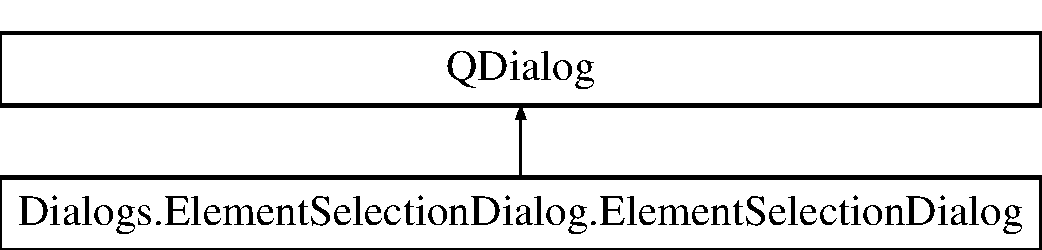
\includegraphics[height=2.000000cm]{classDialogs_1_1ElementSelectionDialog_1_1ElementSelectionDialog}
\end{center}
\end{figure}
\subsection*{Public Member Functions}
\begin{DoxyCompactItemize}
\item 
def \hyperlink{classDialogs_1_1ElementSelectionDialog_1_1ElementSelectionDialog_ac4b575bc1ba5dfdec580cb540f35fa68}{\-\_\-\-\_\-init\-\_\-\-\_\-}
\end{DoxyCompactItemize}
\subsection*{Public Attributes}
\begin{DoxyCompactItemize}
\item 
\hypertarget{classDialogs_1_1ElementSelectionDialog_1_1ElementSelectionDialog_ab4359e72c390640f84f6d753f9e6cb83}{{\bfseries ui}}\label{classDialogs_1_1ElementSelectionDialog_1_1ElementSelectionDialog_ab4359e72c390640f84f6d753f9e6cb83}

\item 
\hypertarget{classDialogs_1_1ElementSelectionDialog_1_1ElementSelectionDialog_a6409795c3364ddfa79b8d225e24a2d93}{{\bfseries element}}\label{classDialogs_1_1ElementSelectionDialog_1_1ElementSelectionDialog_a6409795c3364ddfa79b8d225e24a2d93}

\end{DoxyCompactItemize}


\subsection{Detailed Description}
\begin{DoxyVerb}ElementSelectionDialog opens a periodic table from which user can select
an element.
\end{DoxyVerb}
 

\subsection{Constructor \& Destructor Documentation}
\hypertarget{classDialogs_1_1ElementSelectionDialog_1_1ElementSelectionDialog_ac4b575bc1ba5dfdec580cb540f35fa68}{\index{Dialogs\-::\-Element\-Selection\-Dialog\-::\-Element\-Selection\-Dialog@{Dialogs\-::\-Element\-Selection\-Dialog\-::\-Element\-Selection\-Dialog}!\-\_\-\-\_\-init\-\_\-\-\_\-@{\-\_\-\-\_\-init\-\_\-\-\_\-}}
\index{\-\_\-\-\_\-init\-\_\-\-\_\-@{\-\_\-\-\_\-init\-\_\-\-\_\-}!Dialogs::ElementSelectionDialog::ElementSelectionDialog@{Dialogs\-::\-Element\-Selection\-Dialog\-::\-Element\-Selection\-Dialog}}
\subsubsection[{\-\_\-\-\_\-init\-\_\-\-\_\-}]{\setlength{\rightskip}{0pt plus 5cm}def Dialogs.\-Element\-Selection\-Dialog.\-Element\-Selection\-Dialog.\-\_\-\-\_\-init\-\_\-\-\_\- (
\begin{DoxyParamCaption}
\item[{}]{self}
\end{DoxyParamCaption}
)}}\label{classDialogs_1_1ElementSelectionDialog_1_1ElementSelectionDialog_ac4b575bc1ba5dfdec580cb540f35fa68}
\begin{DoxyVerb}Inits the ElementSelection class
\end{DoxyVerb}
 

The documentation for this class was generated from the following file\-:\begin{DoxyCompactItemize}
\item 
Dialogs/Element\-Selection\-Dialog.\-py\end{DoxyCompactItemize}

\hypertarget{classModules_1_1EnergySpectrum_1_1EnergySpectrum}{\section{Modules.\-Energy\-Spectrum.\-Energy\-Spectrum Class Reference}
\label{classModules_1_1EnergySpectrum_1_1EnergySpectrum}\index{Modules.\-Energy\-Spectrum.\-Energy\-Spectrum@{Modules.\-Energy\-Spectrum.\-Energy\-Spectrum}}
}
\subsection*{Public Member Functions}
\begin{DoxyCompactItemize}
\item 
def \hyperlink{classModules_1_1EnergySpectrum_1_1EnergySpectrum_adeebb674fa3fd402b87abcfe488762d6}{\-\_\-\-\_\-init\-\_\-\-\_\-}
\item 
def \hyperlink{classModules_1_1EnergySpectrum_1_1EnergySpectrum_a97d5455f817511e122cb9451e65ce3c8}{calculate\-\_\-spectrum}
\end{DoxyCompactItemize}


\subsection{Detailed Description}
\begin{DoxyVerb}\end{DoxyVerb}
 

\subsection{Constructor \& Destructor Documentation}
\hypertarget{classModules_1_1EnergySpectrum_1_1EnergySpectrum_adeebb674fa3fd402b87abcfe488762d6}{\index{Modules\-::\-Energy\-Spectrum\-::\-Energy\-Spectrum@{Modules\-::\-Energy\-Spectrum\-::\-Energy\-Spectrum}!\-\_\-\-\_\-init\-\_\-\-\_\-@{\-\_\-\-\_\-init\-\_\-\-\_\-}}
\index{\-\_\-\-\_\-init\-\_\-\-\_\-@{\-\_\-\-\_\-init\-\_\-\-\_\-}!Modules::EnergySpectrum::EnergySpectrum@{Modules\-::\-Energy\-Spectrum\-::\-Energy\-Spectrum}}
\subsubsection[{\-\_\-\-\_\-init\-\_\-\-\_\-}]{\setlength{\rightskip}{0pt plus 5cm}def Modules.\-Energy\-Spectrum.\-Energy\-Spectrum.\-\_\-\-\_\-init\-\_\-\-\_\- (
\begin{DoxyParamCaption}
\item[{}]{self, }
\item[{}]{measurement, }
\item[{}]{cut\-\_\-files, }
\item[{}]{spectrum\-\_\-width, }
\item[{}]{progress\-\_\-bar = {\ttfamily {\bf Null}()}}
\end{DoxyParamCaption}
)}}\label{classModules_1_1EnergySpectrum_1_1EnergySpectrum_adeebb674fa3fd402b87abcfe488762d6}
\begin{DoxyVerb}Inits energy spectrum

Args:
    measurement: A Measurement class object for which Energy Spectrum
         is made.
    cut_files: String list of cut files.
    spectrum_width: Float representing energy spectrum graph width.
    progress_bar: QtWidgets.QProgressBar for GUI (Null class object otherwise).
\end{DoxyVerb}
 

\subsection{Member Function Documentation}
\hypertarget{classModules_1_1EnergySpectrum_1_1EnergySpectrum_a97d5455f817511e122cb9451e65ce3c8}{\index{Modules\-::\-Energy\-Spectrum\-::\-Energy\-Spectrum@{Modules\-::\-Energy\-Spectrum\-::\-Energy\-Spectrum}!calculate\-\_\-spectrum@{calculate\-\_\-spectrum}}
\index{calculate\-\_\-spectrum@{calculate\-\_\-spectrum}!Modules::EnergySpectrum::EnergySpectrum@{Modules\-::\-Energy\-Spectrum\-::\-Energy\-Spectrum}}
\subsubsection[{calculate\-\_\-spectrum}]{\setlength{\rightskip}{0pt plus 5cm}def Modules.\-Energy\-Spectrum.\-Energy\-Spectrum.\-calculate\-\_\-spectrum (
\begin{DoxyParamCaption}
\item[{}]{self}
\end{DoxyParamCaption}
)}}\label{classModules_1_1EnergySpectrum_1_1EnergySpectrum_a97d5455f817511e122cb9451e65ce3c8}
\begin{DoxyVerb}Calculate energy spectrum data from cut files.

Returns list of cut files 
\end{DoxyVerb}
 

The documentation for this class was generated from the following file\-:\begin{DoxyCompactItemize}
\item 
Modules/Energy\-Spectrum.\-py\end{DoxyCompactItemize}

\hypertarget{classDialogs_1_1EnergySpectrumDialog_1_1EnergySpectrumParamsDialog}{\section{Dialogs.\-Energy\-Spectrum\-Dialog.\-Energy\-Spectrum\-Params\-Dialog Class Reference}
\label{classDialogs_1_1EnergySpectrumDialog_1_1EnergySpectrumParamsDialog}\index{Dialogs.\-Energy\-Spectrum\-Dialog.\-Energy\-Spectrum\-Params\-Dialog@{Dialogs.\-Energy\-Spectrum\-Dialog.\-Energy\-Spectrum\-Params\-Dialog}}
}
Inheritance diagram for Dialogs.\-Energy\-Spectrum\-Dialog.\-Energy\-Spectrum\-Params\-Dialog\-:\begin{figure}[H]
\begin{center}
\leavevmode
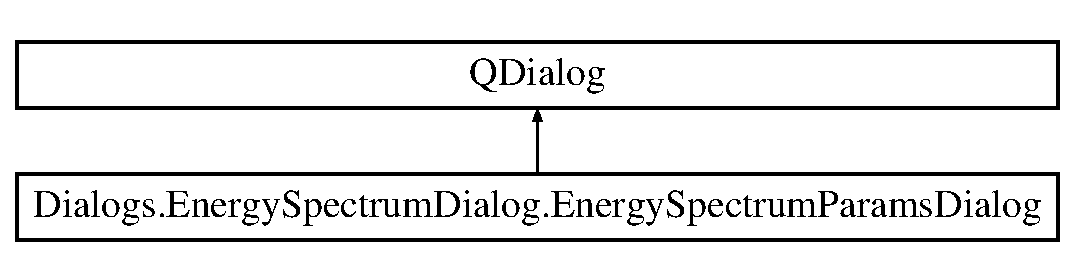
\includegraphics[height=2.000000cm]{classDialogs_1_1EnergySpectrumDialog_1_1EnergySpectrumParamsDialog}
\end{center}
\end{figure}
\subsection*{Public Member Functions}
\begin{DoxyCompactItemize}
\item 
def \hyperlink{classDialogs_1_1EnergySpectrumDialog_1_1EnergySpectrumParamsDialog_aef116ee9f9a1142443dfb8ef6623ddb1}{\-\_\-\-\_\-init\-\_\-\-\_\-}
\end{DoxyCompactItemize}
\subsection*{Public Attributes}
\begin{DoxyCompactItemize}
\item 
\hypertarget{classDialogs_1_1EnergySpectrumDialog_1_1EnergySpectrumParamsDialog_acc5342bc7256c7959dd329d1a85ab50a}{{\bfseries parent}}\label{classDialogs_1_1EnergySpectrumDialog_1_1EnergySpectrumParamsDialog_acc5342bc7256c7959dd329d1a85ab50a}

\item 
\hypertarget{classDialogs_1_1EnergySpectrumDialog_1_1EnergySpectrumParamsDialog_ae2440de847cb63aa6088b266c874f738}{{\bfseries measurement}}\label{classDialogs_1_1EnergySpectrumDialog_1_1EnergySpectrumParamsDialog_ae2440de847cb63aa6088b266c874f738}

\item 
\hypertarget{classDialogs_1_1EnergySpectrumDialog_1_1EnergySpectrumParamsDialog_af74d8d3535de50415f392f68338126f7}{{\bfseries ui}}\label{classDialogs_1_1EnergySpectrumDialog_1_1EnergySpectrumParamsDialog_af74d8d3535de50415f392f68338126f7}

\end{DoxyCompactItemize}
\subsection*{Static Public Attributes}
\begin{DoxyCompactItemize}
\item 
\hypertarget{classDialogs_1_1EnergySpectrumDialog_1_1EnergySpectrumParamsDialog_a7622b9fff7972441b3e6741c56040136}{dictionary {\bfseries checked\-\_\-cuts} = \{\}}\label{classDialogs_1_1EnergySpectrumDialog_1_1EnergySpectrumParamsDialog_a7622b9fff7972441b3e6741c56040136}

\item 
\hypertarget{classDialogs_1_1EnergySpectrumDialog_1_1EnergySpectrumParamsDialog_a59fb4035c2c8f6705aff405ef7ec6ec7}{float {\bfseries bin\-\_\-width} = 0.\-1}\label{classDialogs_1_1EnergySpectrumDialog_1_1EnergySpectrumParamsDialog_a59fb4035c2c8f6705aff405ef7ec6ec7}

\end{DoxyCompactItemize}


\subsection{Constructor \& Destructor Documentation}
\hypertarget{classDialogs_1_1EnergySpectrumDialog_1_1EnergySpectrumParamsDialog_aef116ee9f9a1142443dfb8ef6623ddb1}{\index{Dialogs\-::\-Energy\-Spectrum\-Dialog\-::\-Energy\-Spectrum\-Params\-Dialog@{Dialogs\-::\-Energy\-Spectrum\-Dialog\-::\-Energy\-Spectrum\-Params\-Dialog}!\-\_\-\-\_\-init\-\_\-\-\_\-@{\-\_\-\-\_\-init\-\_\-\-\_\-}}
\index{\-\_\-\-\_\-init\-\_\-\-\_\-@{\-\_\-\-\_\-init\-\_\-\-\_\-}!Dialogs::EnergySpectrumDialog::EnergySpectrumParamsDialog@{Dialogs\-::\-Energy\-Spectrum\-Dialog\-::\-Energy\-Spectrum\-Params\-Dialog}}
\subsubsection[{\-\_\-\-\_\-init\-\_\-\-\_\-}]{\setlength{\rightskip}{0pt plus 5cm}def Dialogs.\-Energy\-Spectrum\-Dialog.\-Energy\-Spectrum\-Params\-Dialog.\-\_\-\-\_\-init\-\_\-\-\_\- (
\begin{DoxyParamCaption}
\item[{}]{self, }
\item[{}]{parent}
\end{DoxyParamCaption}
)}}\label{classDialogs_1_1EnergySpectrumDialog_1_1EnergySpectrumParamsDialog_aef116ee9f9a1142443dfb8ef6623ddb1}
\begin{DoxyVerb}Inits energy spectrum dialog.

Args:
    parent: MeasurementTabWidget
\end{DoxyVerb}
 

The documentation for this class was generated from the following file\-:\begin{DoxyCompactItemize}
\item 
Dialogs/Energy\-Spectrum\-Dialog.\-py\end{DoxyCompactItemize}

\hypertarget{classDialogs_1_1EnergySpectrumDialog_1_1EnergySpectrumWidget}{\section{Dialogs.\-Energy\-Spectrum\-Dialog.\-Energy\-Spectrum\-Widget Class Reference}
\label{classDialogs_1_1EnergySpectrumDialog_1_1EnergySpectrumWidget}\index{Dialogs.\-Energy\-Spectrum\-Dialog.\-Energy\-Spectrum\-Widget@{Dialogs.\-Energy\-Spectrum\-Dialog.\-Energy\-Spectrum\-Widget}}
}
Inheritance diagram for Dialogs.\-Energy\-Spectrum\-Dialog.\-Energy\-Spectrum\-Widget\-:\begin{figure}[H]
\begin{center}
\leavevmode
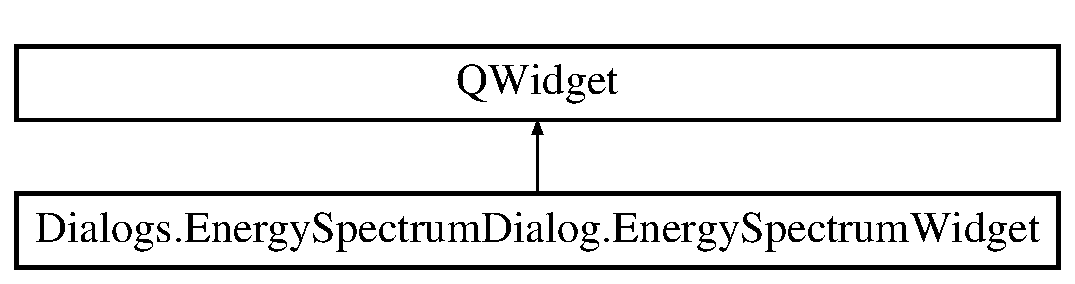
\includegraphics[height=2.000000cm]{classDialogs_1_1EnergySpectrumDialog_1_1EnergySpectrumWidget}
\end{center}
\end{figure}
\subsection*{Public Member Functions}
\begin{DoxyCompactItemize}
\item 
def \hyperlink{classDialogs_1_1EnergySpectrumDialog_1_1EnergySpectrumWidget_a1e0e0c3da1eebe63f9c197ec63be9436}{\-\_\-\-\_\-init\-\_\-\-\_\-}
\item 
def \hyperlink{classDialogs_1_1EnergySpectrumDialog_1_1EnergySpectrumWidget_a65c5bab24a8dc527f2cc996c62c62d16}{delete}
\item 
def \hyperlink{classDialogs_1_1EnergySpectrumDialog_1_1EnergySpectrumWidget_a94de0ccbae352dbd3808d5f183719b58}{close\-Event}
\item 
def \hyperlink{classDialogs_1_1EnergySpectrumDialog_1_1EnergySpectrumWidget_aee32bb81e69c7d5129d0d73a5137d8ee}{save\-\_\-to\-\_\-file}
\end{DoxyCompactItemize}
\subsection*{Public Attributes}
\begin{DoxyCompactItemize}
\item 
\hypertarget{classDialogs_1_1EnergySpectrumDialog_1_1EnergySpectrumWidget_a49930bcc99660a6b29de8a7171ce1b20}{{\bfseries parent}}\label{classDialogs_1_1EnergySpectrumDialog_1_1EnergySpectrumWidget_a49930bcc99660a6b29de8a7171ce1b20}

\item 
\hypertarget{classDialogs_1_1EnergySpectrumDialog_1_1EnergySpectrumWidget_a9edeb56ffca87d290a1ceddad2be22f3}{{\bfseries icon\-\_\-manager}}\label{classDialogs_1_1EnergySpectrumDialog_1_1EnergySpectrumWidget_a9edeb56ffca87d290a1ceddad2be22f3}

\item 
\hypertarget{classDialogs_1_1EnergySpectrumDialog_1_1EnergySpectrumWidget_af04ac1f316285d175ca2322b8640ebfd}{{\bfseries measurement}}\label{classDialogs_1_1EnergySpectrumDialog_1_1EnergySpectrumWidget_af04ac1f316285d175ca2322b8640ebfd}

\item 
\hypertarget{classDialogs_1_1EnergySpectrumDialog_1_1EnergySpectrumWidget_a46dc11b5554684b2a196081cd89807a9}{{\bfseries use\-\_\-cuts}}\label{classDialogs_1_1EnergySpectrumDialog_1_1EnergySpectrumWidget_a46dc11b5554684b2a196081cd89807a9}

\item 
\hypertarget{classDialogs_1_1EnergySpectrumDialog_1_1EnergySpectrumWidget_a12c656e7d5c71f5c6002e1b9141d448e}{{\bfseries width}}\label{classDialogs_1_1EnergySpectrumDialog_1_1EnergySpectrumWidget_a12c656e7d5c71f5c6002e1b9141d448e}

\item 
\hypertarget{classDialogs_1_1EnergySpectrumDialog_1_1EnergySpectrumWidget_a7397547587b6f33b0907858dc74d1fa9}{{\bfseries progress\-\_\-bar}}\label{classDialogs_1_1EnergySpectrumDialog_1_1EnergySpectrumWidget_a7397547587b6f33b0907858dc74d1fa9}

\item 
\hypertarget{classDialogs_1_1EnergySpectrumDialog_1_1EnergySpectrumWidget_a465ba31188aeb082918f75a085d7ac14}{{\bfseries ui}}\label{classDialogs_1_1EnergySpectrumDialog_1_1EnergySpectrumWidget_a465ba31188aeb082918f75a085d7ac14}

\item 
\hypertarget{classDialogs_1_1EnergySpectrumDialog_1_1EnergySpectrumWidget_a03edfefc1c548a9e93a2167693ef655b}{{\bfseries energy\-\_\-spectrum}}\label{classDialogs_1_1EnergySpectrumDialog_1_1EnergySpectrumWidget_a03edfefc1c548a9e93a2167693ef655b}

\item 
\hypertarget{classDialogs_1_1EnergySpectrumDialog_1_1EnergySpectrumWidget_a0e05aa886bb66d9fd8482d4de6f21d45}{{\bfseries energy\-\_\-spectrum\-\_\-data}}\label{classDialogs_1_1EnergySpectrumDialog_1_1EnergySpectrumWidget_a0e05aa886bb66d9fd8482d4de6f21d45}

\item 
\hypertarget{classDialogs_1_1EnergySpectrumDialog_1_1EnergySpectrumWidget_ac151b3c59e72dbb5cbddb7fa596654c1}{{\bfseries matplotlib}}\label{classDialogs_1_1EnergySpectrumDialog_1_1EnergySpectrumWidget_ac151b3c59e72dbb5cbddb7fa596654c1}

\end{DoxyCompactItemize}
\subsection*{Static Public Attributes}
\begin{DoxyCompactItemize}
\item 
\hypertarget{classDialogs_1_1EnergySpectrumDialog_1_1EnergySpectrumWidget_a051f559de9ad5bbe947f7019b099e891}{string {\bfseries save\-\_\-file} = \char`\"{}widget\-\_\-energy\-\_\-spectrum.\-save\char`\"{}}\label{classDialogs_1_1EnergySpectrumDialog_1_1EnergySpectrumWidget_a051f559de9ad5bbe947f7019b099e891}

\end{DoxyCompactItemize}


\subsection{Detailed Description}
\begin{DoxyVerb}Energy spectrum widget which is added to measurement tab.
\end{DoxyVerb}
 

\subsection{Constructor \& Destructor Documentation}
\hypertarget{classDialogs_1_1EnergySpectrumDialog_1_1EnergySpectrumWidget_a1e0e0c3da1eebe63f9c197ec63be9436}{\index{Dialogs\-::\-Energy\-Spectrum\-Dialog\-::\-Energy\-Spectrum\-Widget@{Dialogs\-::\-Energy\-Spectrum\-Dialog\-::\-Energy\-Spectrum\-Widget}!\-\_\-\-\_\-init\-\_\-\-\_\-@{\-\_\-\-\_\-init\-\_\-\-\_\-}}
\index{\-\_\-\-\_\-init\-\_\-\-\_\-@{\-\_\-\-\_\-init\-\_\-\-\_\-}!Dialogs::EnergySpectrumDialog::EnergySpectrumWidget@{Dialogs\-::\-Energy\-Spectrum\-Dialog\-::\-Energy\-Spectrum\-Widget}}
\subsubsection[{\-\_\-\-\_\-init\-\_\-\-\_\-}]{\setlength{\rightskip}{0pt plus 5cm}def Dialogs.\-Energy\-Spectrum\-Dialog.\-Energy\-Spectrum\-Widget.\-\_\-\-\_\-init\-\_\-\-\_\- (
\begin{DoxyParamCaption}
\item[{}]{self, }
\item[{}]{parent, }
\item[{}]{use\-\_\-cuts, }
\item[{}]{width}
\end{DoxyParamCaption}
)}}\label{classDialogs_1_1EnergySpectrumDialog_1_1EnergySpectrumWidget_a1e0e0c3da1eebe63f9c197ec63be9436}
\begin{DoxyVerb}Inits widget.

Args:
    parent: A MeasurementTabWidget.
    use_cuts: A string list representing Cut files.
    width: A float representing Energy Spectrum histogram's bin width.
\end{DoxyVerb}
 

\subsection{Member Function Documentation}
\hypertarget{classDialogs_1_1EnergySpectrumDialog_1_1EnergySpectrumWidget_a94de0ccbae352dbd3808d5f183719b58}{\index{Dialogs\-::\-Energy\-Spectrum\-Dialog\-::\-Energy\-Spectrum\-Widget@{Dialogs\-::\-Energy\-Spectrum\-Dialog\-::\-Energy\-Spectrum\-Widget}!close\-Event@{close\-Event}}
\index{close\-Event@{close\-Event}!Dialogs::EnergySpectrumDialog::EnergySpectrumWidget@{Dialogs\-::\-Energy\-Spectrum\-Dialog\-::\-Energy\-Spectrum\-Widget}}
\subsubsection[{close\-Event}]{\setlength{\rightskip}{0pt plus 5cm}def Dialogs.\-Energy\-Spectrum\-Dialog.\-Energy\-Spectrum\-Widget.\-close\-Event (
\begin{DoxyParamCaption}
\item[{}]{self, }
\item[{}]{evnt}
\end{DoxyParamCaption}
)}}\label{classDialogs_1_1EnergySpectrumDialog_1_1EnergySpectrumWidget_a94de0ccbae352dbd3808d5f183719b58}
\begin{DoxyVerb}Reimplemented method when closing widget.
\end{DoxyVerb}
 \hypertarget{classDialogs_1_1EnergySpectrumDialog_1_1EnergySpectrumWidget_a65c5bab24a8dc527f2cc996c62c62d16}{\index{Dialogs\-::\-Energy\-Spectrum\-Dialog\-::\-Energy\-Spectrum\-Widget@{Dialogs\-::\-Energy\-Spectrum\-Dialog\-::\-Energy\-Spectrum\-Widget}!delete@{delete}}
\index{delete@{delete}!Dialogs::EnergySpectrumDialog::EnergySpectrumWidget@{Dialogs\-::\-Energy\-Spectrum\-Dialog\-::\-Energy\-Spectrum\-Widget}}
\subsubsection[{delete}]{\setlength{\rightskip}{0pt plus 5cm}def Dialogs.\-Energy\-Spectrum\-Dialog.\-Energy\-Spectrum\-Widget.\-delete (
\begin{DoxyParamCaption}
\item[{}]{self}
\end{DoxyParamCaption}
)}}\label{classDialogs_1_1EnergySpectrumDialog_1_1EnergySpectrumWidget_a65c5bab24a8dc527f2cc996c62c62d16}
\begin{DoxyVerb}Delete variables and do clean up.
\end{DoxyVerb}
 \hypertarget{classDialogs_1_1EnergySpectrumDialog_1_1EnergySpectrumWidget_aee32bb81e69c7d5129d0d73a5137d8ee}{\index{Dialogs\-::\-Energy\-Spectrum\-Dialog\-::\-Energy\-Spectrum\-Widget@{Dialogs\-::\-Energy\-Spectrum\-Dialog\-::\-Energy\-Spectrum\-Widget}!save\-\_\-to\-\_\-file@{save\-\_\-to\-\_\-file}}
\index{save\-\_\-to\-\_\-file@{save\-\_\-to\-\_\-file}!Dialogs::EnergySpectrumDialog::EnergySpectrumWidget@{Dialogs\-::\-Energy\-Spectrum\-Dialog\-::\-Energy\-Spectrum\-Widget}}
\subsubsection[{save\-\_\-to\-\_\-file}]{\setlength{\rightskip}{0pt plus 5cm}def Dialogs.\-Energy\-Spectrum\-Dialog.\-Energy\-Spectrum\-Widget.\-save\-\_\-to\-\_\-file (
\begin{DoxyParamCaption}
\item[{}]{self}
\end{DoxyParamCaption}
)}}\label{classDialogs_1_1EnergySpectrumDialog_1_1EnergySpectrumWidget_aee32bb81e69c7d5129d0d73a5137d8ee}
\begin{DoxyVerb}Save object information to file.
\end{DoxyVerb}
 

The documentation for this class was generated from the following file\-:\begin{DoxyCompactItemize}
\item 
Dialogs/Energy\-Spectrum\-Dialog.\-py\end{DoxyCompactItemize}

\hypertarget{classModules_1_1GlobalSettings_1_1GlobalSettings}{\section{Modules.\-Global\-Settings.\-Global\-Settings Class Reference}
\label{classModules_1_1GlobalSettings_1_1GlobalSettings}\index{Modules.\-Global\-Settings.\-Global\-Settings@{Modules.\-Global\-Settings.\-Global\-Settings}}
}
\subsection*{Public Member Functions}
\begin{DoxyCompactItemize}
\item 
def \hyperlink{classModules_1_1GlobalSettings_1_1GlobalSettings_a5374ba8c5adb5cf2626ccc1eed0e1ce7}{\-\_\-\-\_\-init\-\_\-\-\_\-}
\item 
def \hyperlink{classModules_1_1GlobalSettings_1_1GlobalSettings_a722d643c43a7cc6470d04b7fd706837a}{save\-\_\-config}
\item 
def \hyperlink{classModules_1_1GlobalSettings_1_1GlobalSettings_a098f4963e451da611a81247e3f25adf6}{get\-\_\-project\-\_\-directory}
\item 
def \hyperlink{classModules_1_1GlobalSettings_1_1GlobalSettings_ac32a5a4d505958a7159254818559896f}{set\-\_\-project\-\_\-directory}
\item 
def \hyperlink{classModules_1_1GlobalSettings_1_1GlobalSettings_ac55f2e77d5460b80c614cfacc47ca5a3}{get\-\_\-project\-\_\-directory\-\_\-last\-\_\-open}
\item 
def \hyperlink{classModules_1_1GlobalSettings_1_1GlobalSettings_acf0be005c88c958114aefaa627571048}{set\-\_\-project\-\_\-directory\-\_\-last\-\_\-open}
\item 
def \hyperlink{classModules_1_1GlobalSettings_1_1GlobalSettings_a54a0c17fb2b5eb31e2c0fda50662439c}{get\-\_\-efficiency\-\_\-directory}
\item 
def \hyperlink{classModules_1_1GlobalSettings_1_1GlobalSettings_a1a194eba526fbcedaefcef0a531ced1f}{set\-\_\-efficiency\-\_\-directory}
\item 
def \hyperlink{classModules_1_1GlobalSettings_1_1GlobalSettings_aee68a86ff11360bfc66ae6ceb32a8b47}{get\-\_\-efficiencies}
\item 
def \hyperlink{classModules_1_1GlobalSettings_1_1GlobalSettings_abcd6ddfa19369286022b9f6aa4b19c87}{get\-\_\-element\-\_\-colors}
\item 
def \hyperlink{classModules_1_1GlobalSettings_1_1GlobalSettings_aa902fb976071c2eeca3af6b450dee539}{get\-\_\-element\-\_\-color}
\item 
def \hyperlink{classModules_1_1GlobalSettings_1_1GlobalSettings_a72694efed4c7caaaf38928dff89859bf}{set\-\_\-element\-\_\-color}
\item 
def \hyperlink{classModules_1_1GlobalSettings_1_1GlobalSettings_aecf6cc889199c82ace2985eb4049ce66}{get\-\_\-import\-\_\-timing}
\item 
def \hyperlink{classModules_1_1GlobalSettings_1_1GlobalSettings_a6a6f3b0a7666e66add6321419180e707}{set\-\_\-import\-\_\-timing}
\item 
def \hyperlink{classModules_1_1GlobalSettings_1_1GlobalSettings_a61e9047bac694c3a479cc8447448561e}{get\-\_\-import\-\_\-coinc\-\_\-count}
\item 
def \hyperlink{classModules_1_1GlobalSettings_1_1GlobalSettings_a12c0df9c8447f7fb8fe5b9c21830a8be}{set\-\_\-import\-\_\-coinc\-\_\-count}
\item 
def \hyperlink{classModules_1_1GlobalSettings_1_1GlobalSettings_aa5a3529087724e47ebb9539cd35e7d16}{get\-\_\-cross\-\_\-sections\-\_\-text}
\item 
def \hyperlink{classModules_1_1GlobalSettings_1_1GlobalSettings_aafa19f39ff7988b9dea3d3e296069459}{get\-\_\-cross\-\_\-sections}
\item 
def \hyperlink{classModules_1_1GlobalSettings_1_1GlobalSettings_a4dcb908fb101d37717b46ed5541f9dae}{set\-\_\-cross\-\_\-sections}
\item 
def \hyperlink{classModules_1_1GlobalSettings_1_1GlobalSettings_a22623877c3a3a4ab454e40501e5627b1}{is\-\_\-es\-\_\-output\-\_\-saved}
\item 
def \hyperlink{classModules_1_1GlobalSettings_1_1GlobalSettings_ab42ef1299125cf317f18a26061dda685}{set\-\_\-es\-\_\-output\-\_\-saved}
\item 
def \hyperlink{classModules_1_1GlobalSettings_1_1GlobalSettings_af65afa21464f35c1c69b1304112948cc}{get\-\_\-tofe\-\_\-transposed}
\item 
def \hyperlink{classModules_1_1GlobalSettings_1_1GlobalSettings_ab0fbe165feadf2ed0dc2e46934edd66d}{set\-\_\-tofe\-\_\-transposed}
\item 
def \hyperlink{classModules_1_1GlobalSettings_1_1GlobalSettings_ae45c0c955212265f15fcc6e7e4732363}{get\-\_\-tofe\-\_\-invert\-\_\-x}
\item 
def \hyperlink{classModules_1_1GlobalSettings_1_1GlobalSettings_abefbd972722ae65a46a2aa5b1e11861f}{set\-\_\-tofe\-\_\-invert\-\_\-x}
\item 
def \hyperlink{classModules_1_1GlobalSettings_1_1GlobalSettings_a1b9666cc987ac8d7a723871f4e16a845}{get\-\_\-tofe\-\_\-invert\-\_\-y}
\item 
def \hyperlink{classModules_1_1GlobalSettings_1_1GlobalSettings_ad1ba0cbfef67e0bafc377a2db524124b}{set\-\_\-tofe\-\_\-invert\-\_\-y}
\item 
def \hyperlink{classModules_1_1GlobalSettings_1_1GlobalSettings_a47c66d28beec2c660c68ba180115c4e8}{set\-\_\-num\-\_\-iterations}
\item 
def \hyperlink{classModules_1_1GlobalSettings_1_1GlobalSettings_afaa14467b470fe01367f37eae9987eb6}{get\-\_\-num\-\_\-iterations}
\item 
def \hyperlink{classModules_1_1GlobalSettings_1_1GlobalSettings_ae5ab906c18905edd53ebf6befe73b22e}{get\-\_\-tofe\-\_\-color}
\item 
def \hyperlink{classModules_1_1GlobalSettings_1_1GlobalSettings_a855559d711108d84330243885e7019d5}{set\-\_\-tofe\-\_\-color}
\item 
def \hyperlink{classModules_1_1GlobalSettings_1_1GlobalSettings_a34e4a787fd10bb6ef21ad4fdfa9dd71b}{get\-\_\-tofe\-\_\-bin\-\_\-range\-\_\-mode}
\item 
def \hyperlink{classModules_1_1GlobalSettings_1_1GlobalSettings_ad99f233818c997d051e010bffc35fe60}{set\-\_\-tofe\-\_\-bin\-\_\-range\-\_\-mode}
\item 
def \hyperlink{classModules_1_1GlobalSettings_1_1GlobalSettings_ac679c6f87913e2b38f303657ad325214}{get\-\_\-tofe\-\_\-bin\-\_\-range\-\_\-x}
\item 
def \hyperlink{classModules_1_1GlobalSettings_1_1GlobalSettings_a1928dae8b418afe55476d17fb6cfdf94}{set\-\_\-tofe\-\_\-bin\-\_\-range\-\_\-x}
\item 
def \hyperlink{classModules_1_1GlobalSettings_1_1GlobalSettings_ab7a74356cb2841651b8e2abbddb4b290}{get\-\_\-tofe\-\_\-bin\-\_\-range\-\_\-y}
\item 
def \hyperlink{classModules_1_1GlobalSettings_1_1GlobalSettings_ab2eb9ade4f8f1edca2798897672980aa}{set\-\_\-tofe\-\_\-bin\-\_\-range\-\_\-y}
\item 
def \hyperlink{classModules_1_1GlobalSettings_1_1GlobalSettings_a8d78de0571bef813b0d143a9e1e4166c}{get\-\_\-tofe\-\_\-compression\-\_\-x}
\item 
def \hyperlink{classModules_1_1GlobalSettings_1_1GlobalSettings_a18aafdd0ea34347dc6148a8f69f5ca3d}{set\-\_\-tofe\-\_\-compression\-\_\-x}
\item 
def \hyperlink{classModules_1_1GlobalSettings_1_1GlobalSettings_af6314a014a56f85ac31acb3b71386538}{get\-\_\-tofe\-\_\-compression\-\_\-y}
\item 
def \hyperlink{classModules_1_1GlobalSettings_1_1GlobalSettings_a78fb8d4cc5fb6bd135f3ce47fac60fd2}{set\-\_\-tofe\-\_\-compression\-\_\-y}
\end{DoxyCompactItemize}


\subsection{Detailed Description}
\begin{DoxyVerb}Global settings class to handle software settings.
\end{DoxyVerb}
 

\subsection{Constructor \& Destructor Documentation}
\hypertarget{classModules_1_1GlobalSettings_1_1GlobalSettings_a5374ba8c5adb5cf2626ccc1eed0e1ce7}{\index{Modules\-::\-Global\-Settings\-::\-Global\-Settings@{Modules\-::\-Global\-Settings\-::\-Global\-Settings}!\-\_\-\-\_\-init\-\_\-\-\_\-@{\-\_\-\-\_\-init\-\_\-\-\_\-}}
\index{\-\_\-\-\_\-init\-\_\-\-\_\-@{\-\_\-\-\_\-init\-\_\-\-\_\-}!Modules::GlobalSettings::GlobalSettings@{Modules\-::\-Global\-Settings\-::\-Global\-Settings}}
\subsubsection[{\-\_\-\-\_\-init\-\_\-\-\_\-}]{\setlength{\rightskip}{0pt plus 5cm}def Modules.\-Global\-Settings.\-Global\-Settings.\-\_\-\-\_\-init\-\_\-\-\_\- (
\begin{DoxyParamCaption}
\item[{}]{self}
\end{DoxyParamCaption}
)}}\label{classModules_1_1GlobalSettings_1_1GlobalSettings_a5374ba8c5adb5cf2626ccc1eed0e1ce7}
\begin{DoxyVerb}Inits GLobalSettings class.
\end{DoxyVerb}
 

\subsection{Member Function Documentation}
\hypertarget{classModules_1_1GlobalSettings_1_1GlobalSettings_aafa19f39ff7988b9dea3d3e296069459}{\index{Modules\-::\-Global\-Settings\-::\-Global\-Settings@{Modules\-::\-Global\-Settings\-::\-Global\-Settings}!get\-\_\-cross\-\_\-sections@{get\-\_\-cross\-\_\-sections}}
\index{get\-\_\-cross\-\_\-sections@{get\-\_\-cross\-\_\-sections}!Modules::GlobalSettings::GlobalSettings@{Modules\-::\-Global\-Settings\-::\-Global\-Settings}}
\subsubsection[{get\-\_\-cross\-\_\-sections}]{\setlength{\rightskip}{0pt plus 5cm}def Modules.\-Global\-Settings.\-Global\-Settings.\-get\-\_\-cross\-\_\-sections (
\begin{DoxyParamCaption}
\item[{}]{self}
\end{DoxyParamCaption}
)}}\label{classModules_1_1GlobalSettings_1_1GlobalSettings_aafa19f39ff7988b9dea3d3e296069459}
\begin{DoxyVerb}Get cross section model to be used in depth profile.
    
Return:
    Returns an integer representing cross sections flag.
\end{DoxyVerb}
 \hypertarget{classModules_1_1GlobalSettings_1_1GlobalSettings_aa5a3529087724e47ebb9539cd35e7d16}{\index{Modules\-::\-Global\-Settings\-::\-Global\-Settings@{Modules\-::\-Global\-Settings\-::\-Global\-Settings}!get\-\_\-cross\-\_\-sections\-\_\-text@{get\-\_\-cross\-\_\-sections\-\_\-text}}
\index{get\-\_\-cross\-\_\-sections\-\_\-text@{get\-\_\-cross\-\_\-sections\-\_\-text}!Modules::GlobalSettings::GlobalSettings@{Modules\-::\-Global\-Settings\-::\-Global\-Settings}}
\subsubsection[{get\-\_\-cross\-\_\-sections\-\_\-text}]{\setlength{\rightskip}{0pt plus 5cm}def Modules.\-Global\-Settings.\-Global\-Settings.\-get\-\_\-cross\-\_\-sections\-\_\-text (
\begin{DoxyParamCaption}
\item[{}]{self}
\end{DoxyParamCaption}
)}}\label{classModules_1_1GlobalSettings_1_1GlobalSettings_aa5a3529087724e47ebb9539cd35e7d16}
\begin{DoxyVerb}Get cross sections flag as text.

Return:
    Returns the cross sections flag as string
\end{DoxyVerb}
 \hypertarget{classModules_1_1GlobalSettings_1_1GlobalSettings_aee68a86ff11360bfc66ae6ceb32a8b47}{\index{Modules\-::\-Global\-Settings\-::\-Global\-Settings@{Modules\-::\-Global\-Settings\-::\-Global\-Settings}!get\-\_\-efficiencies@{get\-\_\-efficiencies}}
\index{get\-\_\-efficiencies@{get\-\_\-efficiencies}!Modules::GlobalSettings::GlobalSettings@{Modules\-::\-Global\-Settings\-::\-Global\-Settings}}
\subsubsection[{get\-\_\-efficiencies}]{\setlength{\rightskip}{0pt plus 5cm}def Modules.\-Global\-Settings.\-Global\-Settings.\-get\-\_\-efficiencies (
\begin{DoxyParamCaption}
\item[{}]{self}
\end{DoxyParamCaption}
)}}\label{classModules_1_1GlobalSettings_1_1GlobalSettings_aee68a86ff11360bfc66ae6ceb32a8b47}
\begin{DoxyVerb}Get efficiency files that are in efficiency file folder and return
them as a list.

Return:
    Returns a string list of efficiency files.
\end{DoxyVerb}
 \hypertarget{classModules_1_1GlobalSettings_1_1GlobalSettings_a54a0c17fb2b5eb31e2c0fda50662439c}{\index{Modules\-::\-Global\-Settings\-::\-Global\-Settings@{Modules\-::\-Global\-Settings\-::\-Global\-Settings}!get\-\_\-efficiency\-\_\-directory@{get\-\_\-efficiency\-\_\-directory}}
\index{get\-\_\-efficiency\-\_\-directory@{get\-\_\-efficiency\-\_\-directory}!Modules::GlobalSettings::GlobalSettings@{Modules\-::\-Global\-Settings\-::\-Global\-Settings}}
\subsubsection[{get\-\_\-efficiency\-\_\-directory}]{\setlength{\rightskip}{0pt plus 5cm}def Modules.\-Global\-Settings.\-Global\-Settings.\-get\-\_\-efficiency\-\_\-directory (
\begin{DoxyParamCaption}
\item[{}]{self}
\end{DoxyParamCaption}
)}}\label{classModules_1_1GlobalSettings_1_1GlobalSettings_a54a0c17fb2b5eb31e2c0fda50662439c}
\begin{DoxyVerb}Get default efficiency directory.
\end{DoxyVerb}
 \hypertarget{classModules_1_1GlobalSettings_1_1GlobalSettings_aa902fb976071c2eeca3af6b450dee539}{\index{Modules\-::\-Global\-Settings\-::\-Global\-Settings@{Modules\-::\-Global\-Settings\-::\-Global\-Settings}!get\-\_\-element\-\_\-color@{get\-\_\-element\-\_\-color}}
\index{get\-\_\-element\-\_\-color@{get\-\_\-element\-\_\-color}!Modules::GlobalSettings::GlobalSettings@{Modules\-::\-Global\-Settings\-::\-Global\-Settings}}
\subsubsection[{get\-\_\-element\-\_\-color}]{\setlength{\rightskip}{0pt plus 5cm}def Modules.\-Global\-Settings.\-Global\-Settings.\-get\-\_\-element\-\_\-color (
\begin{DoxyParamCaption}
\item[{}]{self, }
\item[{}]{element}
\end{DoxyParamCaption}
)}}\label{classModules_1_1GlobalSettings_1_1GlobalSettings_aa902fb976071c2eeca3af6b450dee539}
\begin{DoxyVerb}Get a specific element's color.

Args:
    element: String representing element name.
    
Return:
    Returns a color (string) for a specific element. 
\end{DoxyVerb}
 \hypertarget{classModules_1_1GlobalSettings_1_1GlobalSettings_abcd6ddfa19369286022b9f6aa4b19c87}{\index{Modules\-::\-Global\-Settings\-::\-Global\-Settings@{Modules\-::\-Global\-Settings\-::\-Global\-Settings}!get\-\_\-element\-\_\-colors@{get\-\_\-element\-\_\-colors}}
\index{get\-\_\-element\-\_\-colors@{get\-\_\-element\-\_\-colors}!Modules::GlobalSettings::GlobalSettings@{Modules\-::\-Global\-Settings\-::\-Global\-Settings}}
\subsubsection[{get\-\_\-element\-\_\-colors}]{\setlength{\rightskip}{0pt plus 5cm}def Modules.\-Global\-Settings.\-Global\-Settings.\-get\-\_\-element\-\_\-colors (
\begin{DoxyParamCaption}
\item[{}]{self}
\end{DoxyParamCaption}
)}}\label{classModules_1_1GlobalSettings_1_1GlobalSettings_abcd6ddfa19369286022b9f6aa4b19c87}
\begin{DoxyVerb}Get all elements' colors.

Return:
    Returns a dictionary of elements' colors.
\end{DoxyVerb}
 \hypertarget{classModules_1_1GlobalSettings_1_1GlobalSettings_a61e9047bac694c3a479cc8447448561e}{\index{Modules\-::\-Global\-Settings\-::\-Global\-Settings@{Modules\-::\-Global\-Settings\-::\-Global\-Settings}!get\-\_\-import\-\_\-coinc\-\_\-count@{get\-\_\-import\-\_\-coinc\-\_\-count}}
\index{get\-\_\-import\-\_\-coinc\-\_\-count@{get\-\_\-import\-\_\-coinc\-\_\-count}!Modules::GlobalSettings::GlobalSettings@{Modules\-::\-Global\-Settings\-::\-Global\-Settings}}
\subsubsection[{get\-\_\-import\-\_\-coinc\-\_\-count}]{\setlength{\rightskip}{0pt plus 5cm}def Modules.\-Global\-Settings.\-Global\-Settings.\-get\-\_\-import\-\_\-coinc\-\_\-count (
\begin{DoxyParamCaption}
\item[{}]{self}
\end{DoxyParamCaption}
)}}\label{classModules_1_1GlobalSettings_1_1GlobalSettings_a61e9047bac694c3a479cc8447448561e}
\begin{DoxyVerb}Get how many coincidences will be collected for timing preview.
    
Return:
    Returns an integer representing coincidence count.
\end{DoxyVerb}
 \hypertarget{classModules_1_1GlobalSettings_1_1GlobalSettings_aecf6cc889199c82ace2985eb4049ce66}{\index{Modules\-::\-Global\-Settings\-::\-Global\-Settings@{Modules\-::\-Global\-Settings\-::\-Global\-Settings}!get\-\_\-import\-\_\-timing@{get\-\_\-import\-\_\-timing}}
\index{get\-\_\-import\-\_\-timing@{get\-\_\-import\-\_\-timing}!Modules::GlobalSettings::GlobalSettings@{Modules\-::\-Global\-Settings\-::\-Global\-Settings}}
\subsubsection[{get\-\_\-import\-\_\-timing}]{\setlength{\rightskip}{0pt plus 5cm}def Modules.\-Global\-Settings.\-Global\-Settings.\-get\-\_\-import\-\_\-timing (
\begin{DoxyParamCaption}
\item[{}]{self, }
\item[{}]{adc}
\end{DoxyParamCaption}
)}}\label{classModules_1_1GlobalSettings_1_1GlobalSettings_aecf6cc889199c82ace2985eb4049ce66}
\begin{DoxyVerb}Get coincidence timings for specific ADC.

Args:
    ADC: An integer representing ADC channel.
    
Return:
    Returns low & high values for coincidence timing.
\end{DoxyVerb}
 \hypertarget{classModules_1_1GlobalSettings_1_1GlobalSettings_afaa14467b470fe01367f37eae9987eb6}{\index{Modules\-::\-Global\-Settings\-::\-Global\-Settings@{Modules\-::\-Global\-Settings\-::\-Global\-Settings}!get\-\_\-num\-\_\-iterations@{get\-\_\-num\-\_\-iterations}}
\index{get\-\_\-num\-\_\-iterations@{get\-\_\-num\-\_\-iterations}!Modules::GlobalSettings::GlobalSettings@{Modules\-::\-Global\-Settings\-::\-Global\-Settings}}
\subsubsection[{get\-\_\-num\-\_\-iterations}]{\setlength{\rightskip}{0pt plus 5cm}def Modules.\-Global\-Settings.\-Global\-Settings.\-get\-\_\-num\-\_\-iterations (
\begin{DoxyParamCaption}
\item[{}]{self}
\end{DoxyParamCaption}
)}}\label{classModules_1_1GlobalSettings_1_1GlobalSettings_afaa14467b470fe01367f37eae9987eb6}
\begin{DoxyVerb}Set the number of iterations erd_depth is to perform

Args:
    value: An integer
\end{DoxyVerb}
 \hypertarget{classModules_1_1GlobalSettings_1_1GlobalSettings_a098f4963e451da611a81247e3f25adf6}{\index{Modules\-::\-Global\-Settings\-::\-Global\-Settings@{Modules\-::\-Global\-Settings\-::\-Global\-Settings}!get\-\_\-project\-\_\-directory@{get\-\_\-project\-\_\-directory}}
\index{get\-\_\-project\-\_\-directory@{get\-\_\-project\-\_\-directory}!Modules::GlobalSettings::GlobalSettings@{Modules\-::\-Global\-Settings\-::\-Global\-Settings}}
\subsubsection[{get\-\_\-project\-\_\-directory}]{\setlength{\rightskip}{0pt plus 5cm}def Modules.\-Global\-Settings.\-Global\-Settings.\-get\-\_\-project\-\_\-directory (
\begin{DoxyParamCaption}
\item[{}]{self}
\end{DoxyParamCaption}
)}}\label{classModules_1_1GlobalSettings_1_1GlobalSettings_a098f4963e451da611a81247e3f25adf6}
\begin{DoxyVerb}Get default project directory.
\end{DoxyVerb}
 \hypertarget{classModules_1_1GlobalSettings_1_1GlobalSettings_ac55f2e77d5460b80c614cfacc47ca5a3}{\index{Modules\-::\-Global\-Settings\-::\-Global\-Settings@{Modules\-::\-Global\-Settings\-::\-Global\-Settings}!get\-\_\-project\-\_\-directory\-\_\-last\-\_\-open@{get\-\_\-project\-\_\-directory\-\_\-last\-\_\-open}}
\index{get\-\_\-project\-\_\-directory\-\_\-last\-\_\-open@{get\-\_\-project\-\_\-directory\-\_\-last\-\_\-open}!Modules::GlobalSettings::GlobalSettings@{Modules\-::\-Global\-Settings\-::\-Global\-Settings}}
\subsubsection[{get\-\_\-project\-\_\-directory\-\_\-last\-\_\-open}]{\setlength{\rightskip}{0pt plus 5cm}def Modules.\-Global\-Settings.\-Global\-Settings.\-get\-\_\-project\-\_\-directory\-\_\-last\-\_\-open (
\begin{DoxyParamCaption}
\item[{}]{self}
\end{DoxyParamCaption}
)}}\label{classModules_1_1GlobalSettings_1_1GlobalSettings_ac55f2e77d5460b80c614cfacc47ca5a3}
\begin{DoxyVerb}Get directory where last project was opened.
\end{DoxyVerb}
 \hypertarget{classModules_1_1GlobalSettings_1_1GlobalSettings_a34e4a787fd10bb6ef21ad4fdfa9dd71b}{\index{Modules\-::\-Global\-Settings\-::\-Global\-Settings@{Modules\-::\-Global\-Settings\-::\-Global\-Settings}!get\-\_\-tofe\-\_\-bin\-\_\-range\-\_\-mode@{get\-\_\-tofe\-\_\-bin\-\_\-range\-\_\-mode}}
\index{get\-\_\-tofe\-\_\-bin\-\_\-range\-\_\-mode@{get\-\_\-tofe\-\_\-bin\-\_\-range\-\_\-mode}!Modules::GlobalSettings::GlobalSettings@{Modules\-::\-Global\-Settings\-::\-Global\-Settings}}
\subsubsection[{get\-\_\-tofe\-\_\-bin\-\_\-range\-\_\-mode}]{\setlength{\rightskip}{0pt plus 5cm}def Modules.\-Global\-Settings.\-Global\-Settings.\-get\-\_\-tofe\-\_\-bin\-\_\-range\-\_\-mode (
\begin{DoxyParamCaption}
\item[{}]{self}
\end{DoxyParamCaption}
)}}\label{classModules_1_1GlobalSettings_1_1GlobalSettings_a34e4a787fd10bb6ef21ad4fdfa9dd71b}
\begin{DoxyVerb}Get ToF-E Histogram bin range mode.
    
Return:
    Returns an integer representing ToF-E histogram bin range mode.
\end{DoxyVerb}
 \hypertarget{classModules_1_1GlobalSettings_1_1GlobalSettings_ac679c6f87913e2b38f303657ad325214}{\index{Modules\-::\-Global\-Settings\-::\-Global\-Settings@{Modules\-::\-Global\-Settings\-::\-Global\-Settings}!get\-\_\-tofe\-\_\-bin\-\_\-range\-\_\-x@{get\-\_\-tofe\-\_\-bin\-\_\-range\-\_\-x}}
\index{get\-\_\-tofe\-\_\-bin\-\_\-range\-\_\-x@{get\-\_\-tofe\-\_\-bin\-\_\-range\-\_\-x}!Modules::GlobalSettings::GlobalSettings@{Modules\-::\-Global\-Settings\-::\-Global\-Settings}}
\subsubsection[{get\-\_\-tofe\-\_\-bin\-\_\-range\-\_\-x}]{\setlength{\rightskip}{0pt plus 5cm}def Modules.\-Global\-Settings.\-Global\-Settings.\-get\-\_\-tofe\-\_\-bin\-\_\-range\-\_\-x (
\begin{DoxyParamCaption}
\item[{}]{self}
\end{DoxyParamCaption}
)}}\label{classModules_1_1GlobalSettings_1_1GlobalSettings_ac679c6f87913e2b38f303657ad325214}
\begin{DoxyVerb}Get ToF-E Histogram X axis bin range.
    
Return:
    Returns an integer representing ToF-E histogram X axis bin range.
\end{DoxyVerb}
 \hypertarget{classModules_1_1GlobalSettings_1_1GlobalSettings_ab7a74356cb2841651b8e2abbddb4b290}{\index{Modules\-::\-Global\-Settings\-::\-Global\-Settings@{Modules\-::\-Global\-Settings\-::\-Global\-Settings}!get\-\_\-tofe\-\_\-bin\-\_\-range\-\_\-y@{get\-\_\-tofe\-\_\-bin\-\_\-range\-\_\-y}}
\index{get\-\_\-tofe\-\_\-bin\-\_\-range\-\_\-y@{get\-\_\-tofe\-\_\-bin\-\_\-range\-\_\-y}!Modules::GlobalSettings::GlobalSettings@{Modules\-::\-Global\-Settings\-::\-Global\-Settings}}
\subsubsection[{get\-\_\-tofe\-\_\-bin\-\_\-range\-\_\-y}]{\setlength{\rightskip}{0pt plus 5cm}def Modules.\-Global\-Settings.\-Global\-Settings.\-get\-\_\-tofe\-\_\-bin\-\_\-range\-\_\-y (
\begin{DoxyParamCaption}
\item[{}]{self}
\end{DoxyParamCaption}
)}}\label{classModules_1_1GlobalSettings_1_1GlobalSettings_ab7a74356cb2841651b8e2abbddb4b290}
\begin{DoxyVerb}Get ToF-E Histogram Y axis bin range.
    
Return:
    Returns an integer representing ToF-E histogram Y axis bin range.
\end{DoxyVerb}
 \hypertarget{classModules_1_1GlobalSettings_1_1GlobalSettings_ae5ab906c18905edd53ebf6befe73b22e}{\index{Modules\-::\-Global\-Settings\-::\-Global\-Settings@{Modules\-::\-Global\-Settings\-::\-Global\-Settings}!get\-\_\-tofe\-\_\-color@{get\-\_\-tofe\-\_\-color}}
\index{get\-\_\-tofe\-\_\-color@{get\-\_\-tofe\-\_\-color}!Modules::GlobalSettings::GlobalSettings@{Modules\-::\-Global\-Settings\-::\-Global\-Settings}}
\subsubsection[{get\-\_\-tofe\-\_\-color}]{\setlength{\rightskip}{0pt plus 5cm}def Modules.\-Global\-Settings.\-Global\-Settings.\-get\-\_\-tofe\-\_\-color (
\begin{DoxyParamCaption}
\item[{}]{self}
\end{DoxyParamCaption}
)}}\label{classModules_1_1GlobalSettings_1_1GlobalSettings_ae5ab906c18905edd53ebf6befe73b22e}
\begin{DoxyVerb}Get color of the ToF-E Histogram.
    
Return:
    Returns a string representing ToF-E histogram color scheme.
\end{DoxyVerb}
 \hypertarget{classModules_1_1GlobalSettings_1_1GlobalSettings_a8d78de0571bef813b0d143a9e1e4166c}{\index{Modules\-::\-Global\-Settings\-::\-Global\-Settings@{Modules\-::\-Global\-Settings\-::\-Global\-Settings}!get\-\_\-tofe\-\_\-compression\-\_\-x@{get\-\_\-tofe\-\_\-compression\-\_\-x}}
\index{get\-\_\-tofe\-\_\-compression\-\_\-x@{get\-\_\-tofe\-\_\-compression\-\_\-x}!Modules::GlobalSettings::GlobalSettings@{Modules\-::\-Global\-Settings\-::\-Global\-Settings}}
\subsubsection[{get\-\_\-tofe\-\_\-compression\-\_\-x}]{\setlength{\rightskip}{0pt plus 5cm}def Modules.\-Global\-Settings.\-Global\-Settings.\-get\-\_\-tofe\-\_\-compression\-\_\-x (
\begin{DoxyParamCaption}
\item[{}]{self}
\end{DoxyParamCaption}
)}}\label{classModules_1_1GlobalSettings_1_1GlobalSettings_a8d78de0571bef813b0d143a9e1e4166c}
\begin{DoxyVerb}Get ToF-E Histogram X axis compression.
    
Return:
    Returns an integer representing ToF-E histogram Y axis compression.
\end{DoxyVerb}
 \hypertarget{classModules_1_1GlobalSettings_1_1GlobalSettings_af6314a014a56f85ac31acb3b71386538}{\index{Modules\-::\-Global\-Settings\-::\-Global\-Settings@{Modules\-::\-Global\-Settings\-::\-Global\-Settings}!get\-\_\-tofe\-\_\-compression\-\_\-y@{get\-\_\-tofe\-\_\-compression\-\_\-y}}
\index{get\-\_\-tofe\-\_\-compression\-\_\-y@{get\-\_\-tofe\-\_\-compression\-\_\-y}!Modules::GlobalSettings::GlobalSettings@{Modules\-::\-Global\-Settings\-::\-Global\-Settings}}
\subsubsection[{get\-\_\-tofe\-\_\-compression\-\_\-y}]{\setlength{\rightskip}{0pt plus 5cm}def Modules.\-Global\-Settings.\-Global\-Settings.\-get\-\_\-tofe\-\_\-compression\-\_\-y (
\begin{DoxyParamCaption}
\item[{}]{self}
\end{DoxyParamCaption}
)}}\label{classModules_1_1GlobalSettings_1_1GlobalSettings_af6314a014a56f85ac31acb3b71386538}
\begin{DoxyVerb}Get ToF-E Histogram Y axis compression.
    
Return:
    Returns an integer representing ToF-E histogram Y axis compression.
\end{DoxyVerb}
 \hypertarget{classModules_1_1GlobalSettings_1_1GlobalSettings_ae45c0c955212265f15fcc6e7e4732363}{\index{Modules\-::\-Global\-Settings\-::\-Global\-Settings@{Modules\-::\-Global\-Settings\-::\-Global\-Settings}!get\-\_\-tofe\-\_\-invert\-\_\-x@{get\-\_\-tofe\-\_\-invert\-\_\-x}}
\index{get\-\_\-tofe\-\_\-invert\-\_\-x@{get\-\_\-tofe\-\_\-invert\-\_\-x}!Modules::GlobalSettings::GlobalSettings@{Modules\-::\-Global\-Settings\-::\-Global\-Settings}}
\subsubsection[{get\-\_\-tofe\-\_\-invert\-\_\-x}]{\setlength{\rightskip}{0pt plus 5cm}def Modules.\-Global\-Settings.\-Global\-Settings.\-get\-\_\-tofe\-\_\-invert\-\_\-x (
\begin{DoxyParamCaption}
\item[{}]{self}
\end{DoxyParamCaption}
)}}\label{classModules_1_1GlobalSettings_1_1GlobalSettings_ae45c0c955212265f15fcc6e7e4732363}
\begin{DoxyVerb}Get boolean if the ToF-E Histogram's X axis is inverted.
    
Return:
    Returns a boolean if the ToF-E Histogram's X axis is inverted.
\end{DoxyVerb}
 \hypertarget{classModules_1_1GlobalSettings_1_1GlobalSettings_a1b9666cc987ac8d7a723871f4e16a845}{\index{Modules\-::\-Global\-Settings\-::\-Global\-Settings@{Modules\-::\-Global\-Settings\-::\-Global\-Settings}!get\-\_\-tofe\-\_\-invert\-\_\-y@{get\-\_\-tofe\-\_\-invert\-\_\-y}}
\index{get\-\_\-tofe\-\_\-invert\-\_\-y@{get\-\_\-tofe\-\_\-invert\-\_\-y}!Modules::GlobalSettings::GlobalSettings@{Modules\-::\-Global\-Settings\-::\-Global\-Settings}}
\subsubsection[{get\-\_\-tofe\-\_\-invert\-\_\-y}]{\setlength{\rightskip}{0pt plus 5cm}def Modules.\-Global\-Settings.\-Global\-Settings.\-get\-\_\-tofe\-\_\-invert\-\_\-y (
\begin{DoxyParamCaption}
\item[{}]{self}
\end{DoxyParamCaption}
)}}\label{classModules_1_1GlobalSettings_1_1GlobalSettings_a1b9666cc987ac8d7a723871f4e16a845}
\begin{DoxyVerb}Get boolean if the ToF-E Histogram's Y axis is inverted.
    
Return:
    Returns a boolean if the ToF-E Histogram's Y axis is inverted.
\end{DoxyVerb}
 \hypertarget{classModules_1_1GlobalSettings_1_1GlobalSettings_af65afa21464f35c1c69b1304112948cc}{\index{Modules\-::\-Global\-Settings\-::\-Global\-Settings@{Modules\-::\-Global\-Settings\-::\-Global\-Settings}!get\-\_\-tofe\-\_\-transposed@{get\-\_\-tofe\-\_\-transposed}}
\index{get\-\_\-tofe\-\_\-transposed@{get\-\_\-tofe\-\_\-transposed}!Modules::GlobalSettings::GlobalSettings@{Modules\-::\-Global\-Settings\-::\-Global\-Settings}}
\subsubsection[{get\-\_\-tofe\-\_\-transposed}]{\setlength{\rightskip}{0pt plus 5cm}def Modules.\-Global\-Settings.\-Global\-Settings.\-get\-\_\-tofe\-\_\-transposed (
\begin{DoxyParamCaption}
\item[{}]{self}
\end{DoxyParamCaption}
)}}\label{classModules_1_1GlobalSettings_1_1GlobalSettings_af65afa21464f35c1c69b1304112948cc}
\begin{DoxyVerb}Get boolean if the ToF-E Histogram is transposed.
    
Return:
    Returns a boolean if the ToF-E Histogram is transposed.
\end{DoxyVerb}
 \hypertarget{classModules_1_1GlobalSettings_1_1GlobalSettings_a22623877c3a3a4ab454e40501e5627b1}{\index{Modules\-::\-Global\-Settings\-::\-Global\-Settings@{Modules\-::\-Global\-Settings\-::\-Global\-Settings}!is\-\_\-es\-\_\-output\-\_\-saved@{is\-\_\-es\-\_\-output\-\_\-saved}}
\index{is\-\_\-es\-\_\-output\-\_\-saved@{is\-\_\-es\-\_\-output\-\_\-saved}!Modules::GlobalSettings::GlobalSettings@{Modules\-::\-Global\-Settings\-::\-Global\-Settings}}
\subsubsection[{is\-\_\-es\-\_\-output\-\_\-saved}]{\setlength{\rightskip}{0pt plus 5cm}def Modules.\-Global\-Settings.\-Global\-Settings.\-is\-\_\-es\-\_\-output\-\_\-saved (
\begin{DoxyParamCaption}
\item[{}]{self}
\end{DoxyParamCaption}
)}}\label{classModules_1_1GlobalSettings_1_1GlobalSettings_a22623877c3a3a4ab454e40501e5627b1}
\begin{DoxyVerb}Is Energy Spectrum output saved or not.
    
Return:
    Returns a boolean representing will Potku save output or not.
\end{DoxyVerb}
 \hypertarget{classModules_1_1GlobalSettings_1_1GlobalSettings_a722d643c43a7cc6470d04b7fd706837a}{\index{Modules\-::\-Global\-Settings\-::\-Global\-Settings@{Modules\-::\-Global\-Settings\-::\-Global\-Settings}!save\-\_\-config@{save\-\_\-config}}
\index{save\-\_\-config@{save\-\_\-config}!Modules::GlobalSettings::GlobalSettings@{Modules\-::\-Global\-Settings\-::\-Global\-Settings}}
\subsubsection[{save\-\_\-config}]{\setlength{\rightskip}{0pt plus 5cm}def Modules.\-Global\-Settings.\-Global\-Settings.\-save\-\_\-config (
\begin{DoxyParamCaption}
\item[{}]{self}
\end{DoxyParamCaption}
)}}\label{classModules_1_1GlobalSettings_1_1GlobalSettings_a722d643c43a7cc6470d04b7fd706837a}
\begin{DoxyVerb}Save current global settings.
\end{DoxyVerb}
 \hypertarget{classModules_1_1GlobalSettings_1_1GlobalSettings_a4dcb908fb101d37717b46ed5541f9dae}{\index{Modules\-::\-Global\-Settings\-::\-Global\-Settings@{Modules\-::\-Global\-Settings\-::\-Global\-Settings}!set\-\_\-cross\-\_\-sections@{set\-\_\-cross\-\_\-sections}}
\index{set\-\_\-cross\-\_\-sections@{set\-\_\-cross\-\_\-sections}!Modules::GlobalSettings::GlobalSettings@{Modules\-::\-Global\-Settings\-::\-Global\-Settings}}
\subsubsection[{set\-\_\-cross\-\_\-sections}]{\setlength{\rightskip}{0pt plus 5cm}def Modules.\-Global\-Settings.\-Global\-Settings.\-set\-\_\-cross\-\_\-sections (
\begin{DoxyParamCaption}
\item[{}]{self, }
\item[{}]{flag}
\end{DoxyParamCaption}
)}}\label{classModules_1_1GlobalSettings_1_1GlobalSettings_a4dcb908fb101d37717b46ed5541f9dae}
\begin{DoxyVerb}Set cross sections used in depth profile to settings.

Args:
    flag: An integer representing cross sections flag.
\end{DoxyVerb}
 \hypertarget{classModules_1_1GlobalSettings_1_1GlobalSettings_a1a194eba526fbcedaefcef0a531ced1f}{\index{Modules\-::\-Global\-Settings\-::\-Global\-Settings@{Modules\-::\-Global\-Settings\-::\-Global\-Settings}!set\-\_\-efficiency\-\_\-directory@{set\-\_\-efficiency\-\_\-directory}}
\index{set\-\_\-efficiency\-\_\-directory@{set\-\_\-efficiency\-\_\-directory}!Modules::GlobalSettings::GlobalSettings@{Modules\-::\-Global\-Settings\-::\-Global\-Settings}}
\subsubsection[{set\-\_\-efficiency\-\_\-directory}]{\setlength{\rightskip}{0pt plus 5cm}def Modules.\-Global\-Settings.\-Global\-Settings.\-set\-\_\-efficiency\-\_\-directory (
\begin{DoxyParamCaption}
\item[{}]{self, }
\item[{}]{directory}
\end{DoxyParamCaption}
)}}\label{classModules_1_1GlobalSettings_1_1GlobalSettings_a1a194eba526fbcedaefcef0a531ced1f}
\begin{DoxyVerb}Save default efficiency directory.

Args:
    directory: A string representing folder where efficiency files are 
       saved in.
\end{DoxyVerb}
 \hypertarget{classModules_1_1GlobalSettings_1_1GlobalSettings_a72694efed4c7caaaf38928dff89859bf}{\index{Modules\-::\-Global\-Settings\-::\-Global\-Settings@{Modules\-::\-Global\-Settings\-::\-Global\-Settings}!set\-\_\-element\-\_\-color@{set\-\_\-element\-\_\-color}}
\index{set\-\_\-element\-\_\-color@{set\-\_\-element\-\_\-color}!Modules::GlobalSettings::GlobalSettings@{Modules\-::\-Global\-Settings\-::\-Global\-Settings}}
\subsubsection[{set\-\_\-element\-\_\-color}]{\setlength{\rightskip}{0pt plus 5cm}def Modules.\-Global\-Settings.\-Global\-Settings.\-set\-\_\-element\-\_\-color (
\begin{DoxyParamCaption}
\item[{}]{self, }
\item[{}]{element, }
\item[{}]{color}
\end{DoxyParamCaption}
)}}\label{classModules_1_1GlobalSettings_1_1GlobalSettings_a72694efed4c7caaaf38928dff89859bf}
\begin{DoxyVerb}Set default color for an element.

Args:
    element: String representing element.
    color: String representing color.
\end{DoxyVerb}
 \hypertarget{classModules_1_1GlobalSettings_1_1GlobalSettings_ab42ef1299125cf317f18a26061dda685}{\index{Modules\-::\-Global\-Settings\-::\-Global\-Settings@{Modules\-::\-Global\-Settings\-::\-Global\-Settings}!set\-\_\-es\-\_\-output\-\_\-saved@{set\-\_\-es\-\_\-output\-\_\-saved}}
\index{set\-\_\-es\-\_\-output\-\_\-saved@{set\-\_\-es\-\_\-output\-\_\-saved}!Modules::GlobalSettings::GlobalSettings@{Modules\-::\-Global\-Settings\-::\-Global\-Settings}}
\subsubsection[{set\-\_\-es\-\_\-output\-\_\-saved}]{\setlength{\rightskip}{0pt plus 5cm}def Modules.\-Global\-Settings.\-Global\-Settings.\-set\-\_\-es\-\_\-output\-\_\-saved (
\begin{DoxyParamCaption}
\item[{}]{self, }
\item[{}]{flag}
\end{DoxyParamCaption}
)}}\label{classModules_1_1GlobalSettings_1_1GlobalSettings_ab42ef1299125cf317f18a26061dda685}
\begin{DoxyVerb}Set whether Energy Spectrum output is saved or not.

Args:
    flag: A boolean representing will Potku save output or not.
\end{DoxyVerb}
 \hypertarget{classModules_1_1GlobalSettings_1_1GlobalSettings_a12c0df9c8447f7fb8fe5b9c21830a8be}{\index{Modules\-::\-Global\-Settings\-::\-Global\-Settings@{Modules\-::\-Global\-Settings\-::\-Global\-Settings}!set\-\_\-import\-\_\-coinc\-\_\-count@{set\-\_\-import\-\_\-coinc\-\_\-count}}
\index{set\-\_\-import\-\_\-coinc\-\_\-count@{set\-\_\-import\-\_\-coinc\-\_\-count}!Modules::GlobalSettings::GlobalSettings@{Modules\-::\-Global\-Settings\-::\-Global\-Settings}}
\subsubsection[{set\-\_\-import\-\_\-coinc\-\_\-count}]{\setlength{\rightskip}{0pt plus 5cm}def Modules.\-Global\-Settings.\-Global\-Settings.\-set\-\_\-import\-\_\-coinc\-\_\-count (
\begin{DoxyParamCaption}
\item[{}]{self, }
\item[{}]{count}
\end{DoxyParamCaption}
)}}\label{classModules_1_1GlobalSettings_1_1GlobalSettings_a12c0df9c8447f7fb8fe5b9c21830a8be}
\begin{DoxyVerb}Set coincidence timings for specific ADC.

Args:
    count: An integer representing coincidence count.
\end{DoxyVerb}
 \hypertarget{classModules_1_1GlobalSettings_1_1GlobalSettings_a6a6f3b0a7666e66add6321419180e707}{\index{Modules\-::\-Global\-Settings\-::\-Global\-Settings@{Modules\-::\-Global\-Settings\-::\-Global\-Settings}!set\-\_\-import\-\_\-timing@{set\-\_\-import\-\_\-timing}}
\index{set\-\_\-import\-\_\-timing@{set\-\_\-import\-\_\-timing}!Modules::GlobalSettings::GlobalSettings@{Modules\-::\-Global\-Settings\-::\-Global\-Settings}}
\subsubsection[{set\-\_\-import\-\_\-timing}]{\setlength{\rightskip}{0pt plus 5cm}def Modules.\-Global\-Settings.\-Global\-Settings.\-set\-\_\-import\-\_\-timing (
\begin{DoxyParamCaption}
\item[{}]{self, }
\item[{}]{adc, }
\item[{}]{low, }
\item[{}]{high}
\end{DoxyParamCaption}
)}}\label{classModules_1_1GlobalSettings_1_1GlobalSettings_a6a6f3b0a7666e66add6321419180e707}
\begin{DoxyVerb}Set coincidence timings for specific ADC.

Args:
    ADC: An integer representing ADC channel.
    low: An integer representing timing low value.
    high: An integer representing timing high value.
\end{DoxyVerb}
 \hypertarget{classModules_1_1GlobalSettings_1_1GlobalSettings_a47c66d28beec2c660c68ba180115c4e8}{\index{Modules\-::\-Global\-Settings\-::\-Global\-Settings@{Modules\-::\-Global\-Settings\-::\-Global\-Settings}!set\-\_\-num\-\_\-iterations@{set\-\_\-num\-\_\-iterations}}
\index{set\-\_\-num\-\_\-iterations@{set\-\_\-num\-\_\-iterations}!Modules::GlobalSettings::GlobalSettings@{Modules\-::\-Global\-Settings\-::\-Global\-Settings}}
\subsubsection[{set\-\_\-num\-\_\-iterations}]{\setlength{\rightskip}{0pt plus 5cm}def Modules.\-Global\-Settings.\-Global\-Settings.\-set\-\_\-num\-\_\-iterations (
\begin{DoxyParamCaption}
\item[{}]{self, }
\item[{}]{value}
\end{DoxyParamCaption}
)}}\label{classModules_1_1GlobalSettings_1_1GlobalSettings_a47c66d28beec2c660c68ba180115c4e8}
\begin{DoxyVerb}Get the number of iterations erd_depth is to perform

Return:
    Returns the number. As an integer.
\end{DoxyVerb}
 \hypertarget{classModules_1_1GlobalSettings_1_1GlobalSettings_ac32a5a4d505958a7159254818559896f}{\index{Modules\-::\-Global\-Settings\-::\-Global\-Settings@{Modules\-::\-Global\-Settings\-::\-Global\-Settings}!set\-\_\-project\-\_\-directory@{set\-\_\-project\-\_\-directory}}
\index{set\-\_\-project\-\_\-directory@{set\-\_\-project\-\_\-directory}!Modules::GlobalSettings::GlobalSettings@{Modules\-::\-Global\-Settings\-::\-Global\-Settings}}
\subsubsection[{set\-\_\-project\-\_\-directory}]{\setlength{\rightskip}{0pt plus 5cm}def Modules.\-Global\-Settings.\-Global\-Settings.\-set\-\_\-project\-\_\-directory (
\begin{DoxyParamCaption}
\item[{}]{self, }
\item[{}]{directory}
\end{DoxyParamCaption}
)}}\label{classModules_1_1GlobalSettings_1_1GlobalSettings_ac32a5a4d505958a7159254818559896f}
\begin{DoxyVerb}Save default project directory.

Args:
    directory: String representing folder where projects will be saved
    by default.
\end{DoxyVerb}
 \hypertarget{classModules_1_1GlobalSettings_1_1GlobalSettings_acf0be005c88c958114aefaa627571048}{\index{Modules\-::\-Global\-Settings\-::\-Global\-Settings@{Modules\-::\-Global\-Settings\-::\-Global\-Settings}!set\-\_\-project\-\_\-directory\-\_\-last\-\_\-open@{set\-\_\-project\-\_\-directory\-\_\-last\-\_\-open}}
\index{set\-\_\-project\-\_\-directory\-\_\-last\-\_\-open@{set\-\_\-project\-\_\-directory\-\_\-last\-\_\-open}!Modules::GlobalSettings::GlobalSettings@{Modules\-::\-Global\-Settings\-::\-Global\-Settings}}
\subsubsection[{set\-\_\-project\-\_\-directory\-\_\-last\-\_\-open}]{\setlength{\rightskip}{0pt plus 5cm}def Modules.\-Global\-Settings.\-Global\-Settings.\-set\-\_\-project\-\_\-directory\-\_\-last\-\_\-open (
\begin{DoxyParamCaption}
\item[{}]{self, }
\item[{}]{directory}
\end{DoxyParamCaption}
)}}\label{classModules_1_1GlobalSettings_1_1GlobalSettings_acf0be005c88c958114aefaa627571048}
\begin{DoxyVerb}Save last opened project directory.

Args:
    directory: String representing project folder.
\end{DoxyVerb}
 \hypertarget{classModules_1_1GlobalSettings_1_1GlobalSettings_ad99f233818c997d051e010bffc35fe60}{\index{Modules\-::\-Global\-Settings\-::\-Global\-Settings@{Modules\-::\-Global\-Settings\-::\-Global\-Settings}!set\-\_\-tofe\-\_\-bin\-\_\-range\-\_\-mode@{set\-\_\-tofe\-\_\-bin\-\_\-range\-\_\-mode}}
\index{set\-\_\-tofe\-\_\-bin\-\_\-range\-\_\-mode@{set\-\_\-tofe\-\_\-bin\-\_\-range\-\_\-mode}!Modules::GlobalSettings::GlobalSettings@{Modules\-::\-Global\-Settings\-::\-Global\-Settings}}
\subsubsection[{set\-\_\-tofe\-\_\-bin\-\_\-range\-\_\-mode}]{\setlength{\rightskip}{0pt plus 5cm}def Modules.\-Global\-Settings.\-Global\-Settings.\-set\-\_\-tofe\-\_\-bin\-\_\-range\-\_\-mode (
\begin{DoxyParamCaption}
\item[{}]{self, }
\item[{}]{value}
\end{DoxyParamCaption}
)}}\label{classModules_1_1GlobalSettings_1_1GlobalSettings_ad99f233818c997d051e010bffc35fe60}
\begin{DoxyVerb}Set ToF-E Histogram bin range automatic or manual.

Args:
    value: An integer representing the mode. 
   Automatic = 0
   Manual = 1
\end{DoxyVerb}
 \hypertarget{classModules_1_1GlobalSettings_1_1GlobalSettings_a1928dae8b418afe55476d17fb6cfdf94}{\index{Modules\-::\-Global\-Settings\-::\-Global\-Settings@{Modules\-::\-Global\-Settings\-::\-Global\-Settings}!set\-\_\-tofe\-\_\-bin\-\_\-range\-\_\-x@{set\-\_\-tofe\-\_\-bin\-\_\-range\-\_\-x}}
\index{set\-\_\-tofe\-\_\-bin\-\_\-range\-\_\-x@{set\-\_\-tofe\-\_\-bin\-\_\-range\-\_\-x}!Modules::GlobalSettings::GlobalSettings@{Modules\-::\-Global\-Settings\-::\-Global\-Settings}}
\subsubsection[{set\-\_\-tofe\-\_\-bin\-\_\-range\-\_\-x}]{\setlength{\rightskip}{0pt plus 5cm}def Modules.\-Global\-Settings.\-Global\-Settings.\-set\-\_\-tofe\-\_\-bin\-\_\-range\-\_\-x (
\begin{DoxyParamCaption}
\item[{}]{self, }
\item[{}]{value\-\_\-min, }
\item[{}]{value\-\_\-max}
\end{DoxyParamCaption}
)}}\label{classModules_1_1GlobalSettings_1_1GlobalSettings_a1928dae8b418afe55476d17fb6cfdf94}
\begin{DoxyVerb}Set ToF-E Histogram X axis bin range.

Args:
    value_min: An integer representing the axis range minimum.
    value_max: An integer representing the axis range maximum.
\end{DoxyVerb}
 \hypertarget{classModules_1_1GlobalSettings_1_1GlobalSettings_ab2eb9ade4f8f1edca2798897672980aa}{\index{Modules\-::\-Global\-Settings\-::\-Global\-Settings@{Modules\-::\-Global\-Settings\-::\-Global\-Settings}!set\-\_\-tofe\-\_\-bin\-\_\-range\-\_\-y@{set\-\_\-tofe\-\_\-bin\-\_\-range\-\_\-y}}
\index{set\-\_\-tofe\-\_\-bin\-\_\-range\-\_\-y@{set\-\_\-tofe\-\_\-bin\-\_\-range\-\_\-y}!Modules::GlobalSettings::GlobalSettings@{Modules\-::\-Global\-Settings\-::\-Global\-Settings}}
\subsubsection[{set\-\_\-tofe\-\_\-bin\-\_\-range\-\_\-y}]{\setlength{\rightskip}{0pt plus 5cm}def Modules.\-Global\-Settings.\-Global\-Settings.\-set\-\_\-tofe\-\_\-bin\-\_\-range\-\_\-y (
\begin{DoxyParamCaption}
\item[{}]{self, }
\item[{}]{value\-\_\-min, }
\item[{}]{value\-\_\-max}
\end{DoxyParamCaption}
)}}\label{classModules_1_1GlobalSettings_1_1GlobalSettings_ab2eb9ade4f8f1edca2798897672980aa}
\begin{DoxyVerb}Set ToF-E Histogram Y axis bin range.

Args:
    value_min: An integer representing the axis range minimum.
    value_max: An integer representing the axis range maximum.
\end{DoxyVerb}
 \hypertarget{classModules_1_1GlobalSettings_1_1GlobalSettings_a855559d711108d84330243885e7019d5}{\index{Modules\-::\-Global\-Settings\-::\-Global\-Settings@{Modules\-::\-Global\-Settings\-::\-Global\-Settings}!set\-\_\-tofe\-\_\-color@{set\-\_\-tofe\-\_\-color}}
\index{set\-\_\-tofe\-\_\-color@{set\-\_\-tofe\-\_\-color}!Modules::GlobalSettings::GlobalSettings@{Modules\-::\-Global\-Settings\-::\-Global\-Settings}}
\subsubsection[{set\-\_\-tofe\-\_\-color}]{\setlength{\rightskip}{0pt plus 5cm}def Modules.\-Global\-Settings.\-Global\-Settings.\-set\-\_\-tofe\-\_\-color (
\begin{DoxyParamCaption}
\item[{}]{self, }
\item[{}]{value}
\end{DoxyParamCaption}
)}}\label{classModules_1_1GlobalSettings_1_1GlobalSettings_a855559d711108d84330243885e7019d5}
\begin{DoxyVerb}Set  color of the ToF-E Histogram.

Args:
    value: A string representing ToF-E histogram color scheme.
\end{DoxyVerb}
 \hypertarget{classModules_1_1GlobalSettings_1_1GlobalSettings_a18aafdd0ea34347dc6148a8f69f5ca3d}{\index{Modules\-::\-Global\-Settings\-::\-Global\-Settings@{Modules\-::\-Global\-Settings\-::\-Global\-Settings}!set\-\_\-tofe\-\_\-compression\-\_\-x@{set\-\_\-tofe\-\_\-compression\-\_\-x}}
\index{set\-\_\-tofe\-\_\-compression\-\_\-x@{set\-\_\-tofe\-\_\-compression\-\_\-x}!Modules::GlobalSettings::GlobalSettings@{Modules\-::\-Global\-Settings\-::\-Global\-Settings}}
\subsubsection[{set\-\_\-tofe\-\_\-compression\-\_\-x}]{\setlength{\rightskip}{0pt plus 5cm}def Modules.\-Global\-Settings.\-Global\-Settings.\-set\-\_\-tofe\-\_\-compression\-\_\-x (
\begin{DoxyParamCaption}
\item[{}]{self, }
\item[{}]{value}
\end{DoxyParamCaption}
)}}\label{classModules_1_1GlobalSettings_1_1GlobalSettings_a18aafdd0ea34347dc6148a8f69f5ca3d}
\begin{DoxyVerb}Set ToF-E Histogram X axis compression.

Args:
    value: An integer representing the axis compression.
\end{DoxyVerb}
 \hypertarget{classModules_1_1GlobalSettings_1_1GlobalSettings_a78fb8d4cc5fb6bd135f3ce47fac60fd2}{\index{Modules\-::\-Global\-Settings\-::\-Global\-Settings@{Modules\-::\-Global\-Settings\-::\-Global\-Settings}!set\-\_\-tofe\-\_\-compression\-\_\-y@{set\-\_\-tofe\-\_\-compression\-\_\-y}}
\index{set\-\_\-tofe\-\_\-compression\-\_\-y@{set\-\_\-tofe\-\_\-compression\-\_\-y}!Modules::GlobalSettings::GlobalSettings@{Modules\-::\-Global\-Settings\-::\-Global\-Settings}}
\subsubsection[{set\-\_\-tofe\-\_\-compression\-\_\-y}]{\setlength{\rightskip}{0pt plus 5cm}def Modules.\-Global\-Settings.\-Global\-Settings.\-set\-\_\-tofe\-\_\-compression\-\_\-y (
\begin{DoxyParamCaption}
\item[{}]{self, }
\item[{}]{value}
\end{DoxyParamCaption}
)}}\label{classModules_1_1GlobalSettings_1_1GlobalSettings_a78fb8d4cc5fb6bd135f3ce47fac60fd2}
\begin{DoxyVerb}Set ToF-E Histogram Y axis compression.

Args:
    value: An integer representing the axis compression.
\end{DoxyVerb}
 \hypertarget{classModules_1_1GlobalSettings_1_1GlobalSettings_abefbd972722ae65a46a2aa5b1e11861f}{\index{Modules\-::\-Global\-Settings\-::\-Global\-Settings@{Modules\-::\-Global\-Settings\-::\-Global\-Settings}!set\-\_\-tofe\-\_\-invert\-\_\-x@{set\-\_\-tofe\-\_\-invert\-\_\-x}}
\index{set\-\_\-tofe\-\_\-invert\-\_\-x@{set\-\_\-tofe\-\_\-invert\-\_\-x}!Modules::GlobalSettings::GlobalSettings@{Modules\-::\-Global\-Settings\-::\-Global\-Settings}}
\subsubsection[{set\-\_\-tofe\-\_\-invert\-\_\-x}]{\setlength{\rightskip}{0pt plus 5cm}def Modules.\-Global\-Settings.\-Global\-Settings.\-set\-\_\-tofe\-\_\-invert\-\_\-x (
\begin{DoxyParamCaption}
\item[{}]{self, }
\item[{}]{value}
\end{DoxyParamCaption}
)}}\label{classModules_1_1GlobalSettings_1_1GlobalSettings_abefbd972722ae65a46a2aa5b1e11861f}
\begin{DoxyVerb}Set if ToF-E histogram's X axis inverted.

Args:
    value: A boolean representing if the ToF-E Histogram's X axis 
   is inverted.
\end{DoxyVerb}
 \hypertarget{classModules_1_1GlobalSettings_1_1GlobalSettings_ad1ba0cbfef67e0bafc377a2db524124b}{\index{Modules\-::\-Global\-Settings\-::\-Global\-Settings@{Modules\-::\-Global\-Settings\-::\-Global\-Settings}!set\-\_\-tofe\-\_\-invert\-\_\-y@{set\-\_\-tofe\-\_\-invert\-\_\-y}}
\index{set\-\_\-tofe\-\_\-invert\-\_\-y@{set\-\_\-tofe\-\_\-invert\-\_\-y}!Modules::GlobalSettings::GlobalSettings@{Modules\-::\-Global\-Settings\-::\-Global\-Settings}}
\subsubsection[{set\-\_\-tofe\-\_\-invert\-\_\-y}]{\setlength{\rightskip}{0pt plus 5cm}def Modules.\-Global\-Settings.\-Global\-Settings.\-set\-\_\-tofe\-\_\-invert\-\_\-y (
\begin{DoxyParamCaption}
\item[{}]{self, }
\item[{}]{value}
\end{DoxyParamCaption}
)}}\label{classModules_1_1GlobalSettings_1_1GlobalSettings_ad1ba0cbfef67e0bafc377a2db524124b}
\begin{DoxyVerb}Set if ToF-E histogram's Y axis inverted.

Args:
    value: A boolean representing if the ToF-E Histogram's Y axis 
   is inverted.
\end{DoxyVerb}
 \hypertarget{classModules_1_1GlobalSettings_1_1GlobalSettings_ab0fbe165feadf2ed0dc2e46934edd66d}{\index{Modules\-::\-Global\-Settings\-::\-Global\-Settings@{Modules\-::\-Global\-Settings\-::\-Global\-Settings}!set\-\_\-tofe\-\_\-transposed@{set\-\_\-tofe\-\_\-transposed}}
\index{set\-\_\-tofe\-\_\-transposed@{set\-\_\-tofe\-\_\-transposed}!Modules::GlobalSettings::GlobalSettings@{Modules\-::\-Global\-Settings\-::\-Global\-Settings}}
\subsubsection[{set\-\_\-tofe\-\_\-transposed}]{\setlength{\rightskip}{0pt plus 5cm}def Modules.\-Global\-Settings.\-Global\-Settings.\-set\-\_\-tofe\-\_\-transposed (
\begin{DoxyParamCaption}
\item[{}]{self, }
\item[{}]{value}
\end{DoxyParamCaption}
)}}\label{classModules_1_1GlobalSettings_1_1GlobalSettings_ab0fbe165feadf2ed0dc2e46934edd66d}
\begin{DoxyVerb}Set if ToF-E histogram is transposed.

Args:
    value: A boolean representing if the ToF-E Histogram's X axis 
   is inverted.
\end{DoxyVerb}
 

The documentation for this class was generated from the following file\-:\begin{DoxyCompactItemize}
\item 
Modules/Global\-Settings.\-py\end{DoxyCompactItemize}

\hypertarget{classDialogs_1_1GlobalSettingsDialog_1_1GlobalSettingsDialog}{\section{Dialogs.\-Global\-Settings\-Dialog.\-Global\-Settings\-Dialog Class Reference}
\label{classDialogs_1_1GlobalSettingsDialog_1_1GlobalSettingsDialog}\index{Dialogs.\-Global\-Settings\-Dialog.\-Global\-Settings\-Dialog@{Dialogs.\-Global\-Settings\-Dialog.\-Global\-Settings\-Dialog}}
}
Inheritance diagram for Dialogs.\-Global\-Settings\-Dialog.\-Global\-Settings\-Dialog\-:\begin{figure}[H]
\begin{center}
\leavevmode
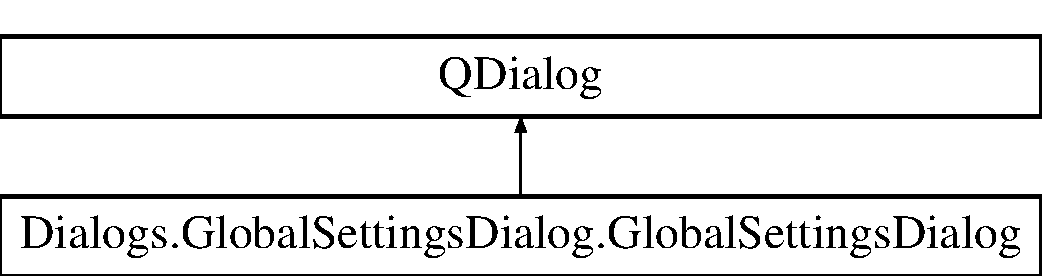
\includegraphics[height=2.000000cm]{classDialogs_1_1GlobalSettingsDialog_1_1GlobalSettingsDialog}
\end{center}
\end{figure}
\subsection*{Public Member Functions}
\begin{DoxyCompactItemize}
\item 
def \hyperlink{classDialogs_1_1GlobalSettingsDialog_1_1GlobalSettingsDialog_a9522566c5d137175f043877d821fdb19}{\-\_\-\-\_\-init\-\_\-\-\_\-}
\end{DoxyCompactItemize}
\subsection*{Public Attributes}
\begin{DoxyCompactItemize}
\item 
\hypertarget{classDialogs_1_1GlobalSettingsDialog_1_1GlobalSettingsDialog_a4b45d9d073d105d1430ca47021365110}{{\bfseries masses}}\label{classDialogs_1_1GlobalSettingsDialog_1_1GlobalSettingsDialog_a4b45d9d073d105d1430ca47021365110}

\item 
\hypertarget{classDialogs_1_1GlobalSettingsDialog_1_1GlobalSettingsDialog_af95fecda58868341ee82aa28b099ee82}{{\bfseries settings}}\label{classDialogs_1_1GlobalSettingsDialog_1_1GlobalSettingsDialog_af95fecda58868341ee82aa28b099ee82}

\item 
\hypertarget{classDialogs_1_1GlobalSettingsDialog_1_1GlobalSettingsDialog_a28f27e885f9ea23e376192fb2ba9ea9e}{{\bfseries ui}}\label{classDialogs_1_1GlobalSettingsDialog_1_1GlobalSettingsDialog_a28f27e885f9ea23e376192fb2ba9ea9e}

\item 
\hypertarget{classDialogs_1_1GlobalSettingsDialog_1_1GlobalSettingsDialog_a7cbf5444a8338bcfcf2fd42bf400085e}{{\bfseries color}}\label{classDialogs_1_1GlobalSettingsDialog_1_1GlobalSettingsDialog_a7cbf5444a8338bcfcf2fd42bf400085e}

\end{DoxyCompactItemize}


\subsection{Constructor \& Destructor Documentation}
\hypertarget{classDialogs_1_1GlobalSettingsDialog_1_1GlobalSettingsDialog_a9522566c5d137175f043877d821fdb19}{\index{Dialogs\-::\-Global\-Settings\-Dialog\-::\-Global\-Settings\-Dialog@{Dialogs\-::\-Global\-Settings\-Dialog\-::\-Global\-Settings\-Dialog}!\-\_\-\-\_\-init\-\_\-\-\_\-@{\-\_\-\-\_\-init\-\_\-\-\_\-}}
\index{\-\_\-\-\_\-init\-\_\-\-\_\-@{\-\_\-\-\_\-init\-\_\-\-\_\-}!Dialogs::GlobalSettingsDialog::GlobalSettingsDialog@{Dialogs\-::\-Global\-Settings\-Dialog\-::\-Global\-Settings\-Dialog}}
\subsubsection[{\-\_\-\-\_\-init\-\_\-\-\_\-}]{\setlength{\rightskip}{0pt plus 5cm}def Dialogs.\-Global\-Settings\-Dialog.\-Global\-Settings\-Dialog.\-\_\-\-\_\-init\-\_\-\-\_\- (
\begin{DoxyParamCaption}
\item[{}]{self, }
\item[{}]{masses, }
\item[{}]{settings}
\end{DoxyParamCaption}
)}}\label{classDialogs_1_1GlobalSettingsDialog_1_1GlobalSettingsDialog_a9522566c5d137175f043877d821fdb19}
\begin{DoxyVerb}Constructor for the program
\end{DoxyVerb}
 

The documentation for this class was generated from the following file\-:\begin{DoxyCompactItemize}
\item 
Dialogs/Global\-Settings\-Dialog.\-py\end{DoxyCompactItemize}

\hypertarget{classDialogs_1_1GraphIgnoreElements_1_1GraphIgnoreElements}{\section{Dialogs.\-Graph\-Ignore\-Elements.\-Graph\-Ignore\-Elements Class Reference}
\label{classDialogs_1_1GraphIgnoreElements_1_1GraphIgnoreElements}\index{Dialogs.\-Graph\-Ignore\-Elements.\-Graph\-Ignore\-Elements@{Dialogs.\-Graph\-Ignore\-Elements.\-Graph\-Ignore\-Elements}}
}
Inheritance diagram for Dialogs.\-Graph\-Ignore\-Elements.\-Graph\-Ignore\-Elements\-:\begin{figure}[H]
\begin{center}
\leavevmode
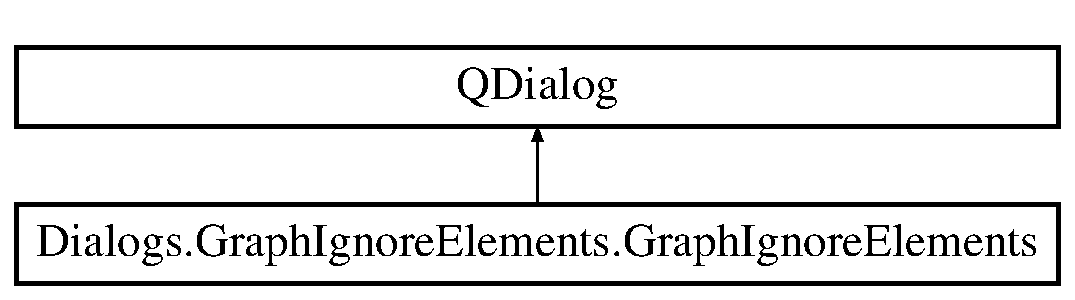
\includegraphics[height=2.000000cm]{classDialogs_1_1GraphIgnoreElements_1_1GraphIgnoreElements}
\end{center}
\end{figure}
\subsection*{Public Member Functions}
\begin{DoxyCompactItemize}
\item 
def \hyperlink{classDialogs_1_1GraphIgnoreElements_1_1GraphIgnoreElements_a0c77514d612b59ba6295debed0d3664b}{\-\_\-\-\_\-init\-\_\-\-\_\-}
\end{DoxyCompactItemize}
\subsection*{Public Attributes}
\begin{DoxyCompactItemize}
\item 
\hypertarget{classDialogs_1_1GraphIgnoreElements_1_1GraphIgnoreElements_ab510440fc16701b8f73387c5ad903235}{{\bfseries ignored\-\_\-elements}}\label{classDialogs_1_1GraphIgnoreElements_1_1GraphIgnoreElements_ab510440fc16701b8f73387c5ad903235}

\end{DoxyCompactItemize}


\subsection{Constructor \& Destructor Documentation}
\hypertarget{classDialogs_1_1GraphIgnoreElements_1_1GraphIgnoreElements_a0c77514d612b59ba6295debed0d3664b}{\index{Dialogs\-::\-Graph\-Ignore\-Elements\-::\-Graph\-Ignore\-Elements@{Dialogs\-::\-Graph\-Ignore\-Elements\-::\-Graph\-Ignore\-Elements}!\-\_\-\-\_\-init\-\_\-\-\_\-@{\-\_\-\-\_\-init\-\_\-\-\_\-}}
\index{\-\_\-\-\_\-init\-\_\-\-\_\-@{\-\_\-\-\_\-init\-\_\-\-\_\-}!Dialogs::GraphIgnoreElements::GraphIgnoreElements@{Dialogs\-::\-Graph\-Ignore\-Elements\-::\-Graph\-Ignore\-Elements}}
\subsubsection[{\-\_\-\-\_\-init\-\_\-\-\_\-}]{\setlength{\rightskip}{0pt plus 5cm}def Dialogs.\-Graph\-Ignore\-Elements.\-Graph\-Ignore\-Elements.\-\_\-\-\_\-init\-\_\-\-\_\- (
\begin{DoxyParamCaption}
\item[{}]{self, }
\item[{}]{elements, }
\item[{}]{ignored}
\end{DoxyParamCaption}
)}}\label{classDialogs_1_1GraphIgnoreElements_1_1GraphIgnoreElements_a0c77514d612b59ba6295debed0d3664b}
\begin{DoxyVerb}Init the dialog.

Args:
    elements: A list of elements in Depth Profile.
    ignored: A list of elements ignored previously for ratio calculation.
\end{DoxyVerb}
 

The documentation for this class was generated from the following file\-:\begin{DoxyCompactItemize}
\item 
Dialogs/Graph\-Ignore\-Elements.\-py\end{DoxyCompactItemize}

\hypertarget{classModules_1_1IconManager_1_1IconManager}{\section{Modules.\-Icon\-Manager.\-Icon\-Manager Class Reference}
\label{classModules_1_1IconManager_1_1IconManager}\index{Modules.\-Icon\-Manager.\-Icon\-Manager@{Modules.\-Icon\-Manager.\-Icon\-Manager}}
}
\subsection*{Public Member Functions}
\begin{DoxyCompactItemize}
\item 
def \hyperlink{classModules_1_1IconManager_1_1IconManager_ab7eeb7278a08345db101b6194a2cc927}{\-\_\-\-\_\-init\-\_\-\-\_\-}
\item 
def \hyperlink{classModules_1_1IconManager_1_1IconManager_a572f242d458eede934e145069b43b633}{get\-\_\-icon}
\item 
def \hyperlink{classModules_1_1IconManager_1_1IconManager_ae715a41265e8b30f9025642671787a8e}{set\-\_\-icon}
\end{DoxyCompactItemize}


\subsection{Detailed Description}
\begin{DoxyVerb}Icon manager class to handle all icons for the program.
\end{DoxyVerb}
 

\subsection{Constructor \& Destructor Documentation}
\hypertarget{classModules_1_1IconManager_1_1IconManager_ab7eeb7278a08345db101b6194a2cc927}{\index{Modules\-::\-Icon\-Manager\-::\-Icon\-Manager@{Modules\-::\-Icon\-Manager\-::\-Icon\-Manager}!\-\_\-\-\_\-init\-\_\-\-\_\-@{\-\_\-\-\_\-init\-\_\-\-\_\-}}
\index{\-\_\-\-\_\-init\-\_\-\-\_\-@{\-\_\-\-\_\-init\-\_\-\-\_\-}!Modules::IconManager::IconManager@{Modules\-::\-Icon\-Manager\-::\-Icon\-Manager}}
\subsubsection[{\-\_\-\-\_\-init\-\_\-\-\_\-}]{\setlength{\rightskip}{0pt plus 5cm}def Modules.\-Icon\-Manager.\-Icon\-Manager.\-\_\-\-\_\-init\-\_\-\-\_\- (
\begin{DoxyParamCaption}
\item[{}]{self}
\end{DoxyParamCaption}
)}}\label{classModules_1_1IconManager_1_1IconManager_ab7eeb7278a08345db101b6194a2cc927}
\begin{DoxyVerb}Inits IconManager class.
\end{DoxyVerb}
 

\subsection{Member Function Documentation}
\hypertarget{classModules_1_1IconManager_1_1IconManager_a572f242d458eede934e145069b43b633}{\index{Modules\-::\-Icon\-Manager\-::\-Icon\-Manager@{Modules\-::\-Icon\-Manager\-::\-Icon\-Manager}!get\-\_\-icon@{get\-\_\-icon}}
\index{get\-\_\-icon@{get\-\_\-icon}!Modules::IconManager::IconManager@{Modules\-::\-Icon\-Manager\-::\-Icon\-Manager}}
\subsubsection[{get\-\_\-icon}]{\setlength{\rightskip}{0pt plus 5cm}def Modules.\-Icon\-Manager.\-Icon\-Manager.\-get\-\_\-icon (
\begin{DoxyParamCaption}
\item[{}]{self, }
\item[{}]{icon\-\_\-name}
\end{DoxyParamCaption}
)}}\label{classModules_1_1IconManager_1_1IconManager_a572f242d458eede934e145069b43b633}
\begin{DoxyVerb}Get specific icon.

Args:
    icon_name: String representing icon file name.
    
Return:
    Returns QtGui.QIcon of icon_name and empty icon if not found.
\end{DoxyVerb}
 \hypertarget{classModules_1_1IconManager_1_1IconManager_ae715a41265e8b30f9025642671787a8e}{\index{Modules\-::\-Icon\-Manager\-::\-Icon\-Manager@{Modules\-::\-Icon\-Manager\-::\-Icon\-Manager}!set\-\_\-icon@{set\-\_\-icon}}
\index{set\-\_\-icon@{set\-\_\-icon}!Modules::IconManager::IconManager@{Modules\-::\-Icon\-Manager\-::\-Icon\-Manager}}
\subsubsection[{set\-\_\-icon}]{\setlength{\rightskip}{0pt plus 5cm}def Modules.\-Icon\-Manager.\-Icon\-Manager.\-set\-\_\-icon (
\begin{DoxyParamCaption}
\item[{}]{self, }
\item[{}]{target, }
\item[{}]{icon\-\_\-name, }
\item[{}]{size = {\ttfamily (20,~20}}
\end{DoxyParamCaption}
)}}\label{classModules_1_1IconManager_1_1IconManager_ae715a41265e8b30f9025642671787a8e}
\begin{DoxyVerb}Set icon (icon_name) to target.

Args:
    target: QtGui element that has icon. (setIcon method)
    icon_name: String representing filename of the icon.
\end{DoxyVerb}
 

The documentation for this class was generated from the following file\-:\begin{DoxyCompactItemize}
\item 
Modules/Icon\-Manager.\-py\end{DoxyCompactItemize}

\hypertarget{classDialogs_1_1ImportMeasurementBinary_1_1ImportDialogBinary}{\section{Dialogs.\-Import\-Measurement\-Binary.\-Import\-Dialog\-Binary Class Reference}
\label{classDialogs_1_1ImportMeasurementBinary_1_1ImportDialogBinary}\index{Dialogs.\-Import\-Measurement\-Binary.\-Import\-Dialog\-Binary@{Dialogs.\-Import\-Measurement\-Binary.\-Import\-Dialog\-Binary}}
}
Inheritance diagram for Dialogs.\-Import\-Measurement\-Binary.\-Import\-Dialog\-Binary\-:\begin{figure}[H]
\begin{center}
\leavevmode
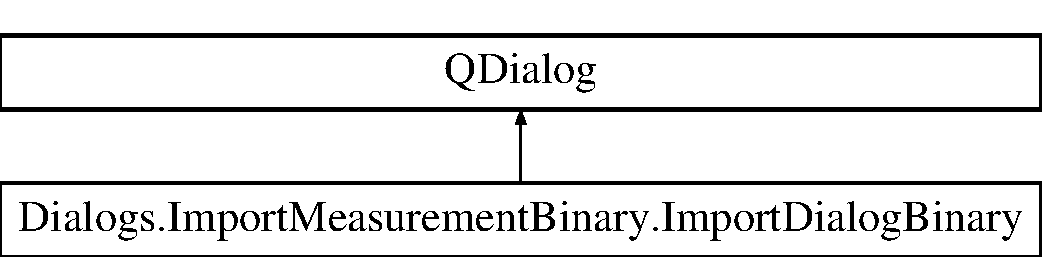
\includegraphics[height=2.000000cm]{classDialogs_1_1ImportMeasurementBinary_1_1ImportDialogBinary}
\end{center}
\end{figure}
\subsection*{Public Member Functions}
\begin{DoxyCompactItemize}
\item 
def \hyperlink{classDialogs_1_1ImportMeasurementBinary_1_1ImportDialogBinary_a9aaaf65a7428c5b1179b7fc0a8609cdb}{\-\_\-\-\_\-init\-\_\-\-\_\-}
\end{DoxyCompactItemize}
\subsection*{Public Attributes}
\begin{DoxyCompactItemize}
\item 
\hypertarget{classDialogs_1_1ImportMeasurementBinary_1_1ImportDialogBinary_aaae1d38eee314ce24667545682f2160c}{{\bfseries imported}}\label{classDialogs_1_1ImportMeasurementBinary_1_1ImportDialogBinary_aaae1d38eee314ce24667545682f2160c}

\end{DoxyCompactItemize}


\subsection{Detailed Description}
\begin{DoxyVerb}Binary measurement importing class.
\end{DoxyVerb}
 

\subsection{Constructor \& Destructor Documentation}
\hypertarget{classDialogs_1_1ImportMeasurementBinary_1_1ImportDialogBinary_a9aaaf65a7428c5b1179b7fc0a8609cdb}{\index{Dialogs\-::\-Import\-Measurement\-Binary\-::\-Import\-Dialog\-Binary@{Dialogs\-::\-Import\-Measurement\-Binary\-::\-Import\-Dialog\-Binary}!\-\_\-\-\_\-init\-\_\-\-\_\-@{\-\_\-\-\_\-init\-\_\-\-\_\-}}
\index{\-\_\-\-\_\-init\-\_\-\-\_\-@{\-\_\-\-\_\-init\-\_\-\-\_\-}!Dialogs::ImportMeasurementBinary::ImportDialogBinary@{Dialogs\-::\-Import\-Measurement\-Binary\-::\-Import\-Dialog\-Binary}}
\subsubsection[{\-\_\-\-\_\-init\-\_\-\-\_\-}]{\setlength{\rightskip}{0pt plus 5cm}def Dialogs.\-Import\-Measurement\-Binary.\-Import\-Dialog\-Binary.\-\_\-\-\_\-init\-\_\-\-\_\- (
\begin{DoxyParamCaption}
\item[{}]{self, }
\item[{}]{project, }
\item[{}]{icon\-\_\-manager, }
\item[{}]{statusbar, }
\item[{}]{parent}
\end{DoxyParamCaption}
)}}\label{classDialogs_1_1ImportMeasurementBinary_1_1ImportDialogBinary_a9aaaf65a7428c5b1179b7fc0a8609cdb}
\begin{DoxyVerb}Init binary measurement import dialog.
\end{DoxyVerb}
 

The documentation for this class was generated from the following file\-:\begin{DoxyCompactItemize}
\item 
Dialogs/Import\-Measurement\-Binary.\-py\end{DoxyCompactItemize}

\hypertarget{classDialogs_1_1ImportMeasurementDialog_1_1ImportMeasurementsDialog}{\section{Dialogs.\-Import\-Measurement\-Dialog.\-Import\-Measurements\-Dialog Class Reference}
\label{classDialogs_1_1ImportMeasurementDialog_1_1ImportMeasurementsDialog}\index{Dialogs.\-Import\-Measurement\-Dialog.\-Import\-Measurements\-Dialog@{Dialogs.\-Import\-Measurement\-Dialog.\-Import\-Measurements\-Dialog}}
}
Inheritance diagram for Dialogs.\-Import\-Measurement\-Dialog.\-Import\-Measurements\-Dialog\-:\begin{figure}[H]
\begin{center}
\leavevmode
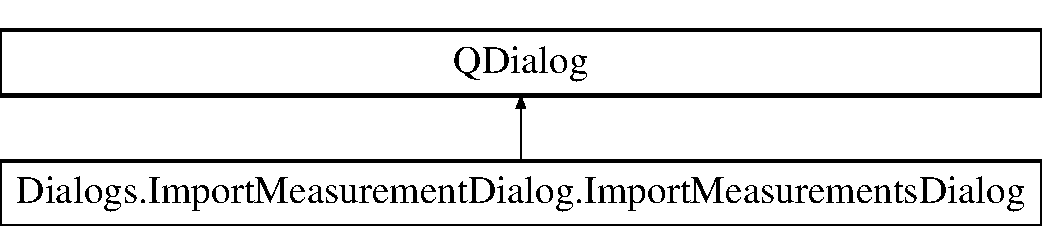
\includegraphics[height=2.000000cm]{classDialogs_1_1ImportMeasurementDialog_1_1ImportMeasurementsDialog}
\end{center}
\end{figure}
\subsection*{Public Member Functions}
\begin{DoxyCompactItemize}
\item 
def \hyperlink{classDialogs_1_1ImportMeasurementDialog_1_1ImportMeasurementsDialog_a9c8cfb8e464c19582f50bd8c2be40078}{\-\_\-\-\_\-init\-\_\-\-\_\-}
\end{DoxyCompactItemize}
\subsection*{Public Attributes}
\begin{DoxyCompactItemize}
\item 
\hypertarget{classDialogs_1_1ImportMeasurementDialog_1_1ImportMeasurementsDialog_af3f60ce8c50e9e868792b2c7d058d3df}{{\bfseries project}}\label{classDialogs_1_1ImportMeasurementDialog_1_1ImportMeasurementsDialog_af3f60ce8c50e9e868792b2c7d058d3df}

\item 
\hypertarget{classDialogs_1_1ImportMeasurementDialog_1_1ImportMeasurementsDialog_a6c8f9a9fd21d3af7290ff28870b46b7f}{{\bfseries statusbar}}\label{classDialogs_1_1ImportMeasurementDialog_1_1ImportMeasurementsDialog_a6c8f9a9fd21d3af7290ff28870b46b7f}

\item 
\hypertarget{classDialogs_1_1ImportMeasurementDialog_1_1ImportMeasurementsDialog_aeaedfe3cfa81f38c4474717e30add092}{{\bfseries parent}}\label{classDialogs_1_1ImportMeasurementDialog_1_1ImportMeasurementsDialog_aeaedfe3cfa81f38c4474717e30add092}

\item 
\hypertarget{classDialogs_1_1ImportMeasurementDialog_1_1ImportMeasurementsDialog_ac9c55bb602f2562a96c2001cc0466096}{{\bfseries global\-\_\-settings}}\label{classDialogs_1_1ImportMeasurementDialog_1_1ImportMeasurementsDialog_ac9c55bb602f2562a96c2001cc0466096}

\item 
\hypertarget{classDialogs_1_1ImportMeasurementDialog_1_1ImportMeasurementsDialog_aba577d94f9a5b1aa27e77e573a3e9562}{{\bfseries imported}}\label{classDialogs_1_1ImportMeasurementDialog_1_1ImportMeasurementsDialog_aba577d94f9a5b1aa27e77e573a3e9562}

\item 
\hypertarget{classDialogs_1_1ImportMeasurementDialog_1_1ImportMeasurementsDialog_adc386c27f53efe3fdbac4165e540872d}{{\bfseries adc\-\_\-occurance}}\label{classDialogs_1_1ImportMeasurementDialog_1_1ImportMeasurementsDialog_adc386c27f53efe3fdbac4165e540872d}

\end{DoxyCompactItemize}


\subsection{Detailed Description}
\begin{DoxyVerb}Measurement importing class. Used to import measurement data
from detecting unit into potku.
\end{DoxyVerb}
 

\subsection{Constructor \& Destructor Documentation}
\hypertarget{classDialogs_1_1ImportMeasurementDialog_1_1ImportMeasurementsDialog_a9c8cfb8e464c19582f50bd8c2be40078}{\index{Dialogs\-::\-Import\-Measurement\-Dialog\-::\-Import\-Measurements\-Dialog@{Dialogs\-::\-Import\-Measurement\-Dialog\-::\-Import\-Measurements\-Dialog}!\-\_\-\-\_\-init\-\_\-\-\_\-@{\-\_\-\-\_\-init\-\_\-\-\_\-}}
\index{\-\_\-\-\_\-init\-\_\-\-\_\-@{\-\_\-\-\_\-init\-\_\-\-\_\-}!Dialogs::ImportMeasurementDialog::ImportMeasurementsDialog@{Dialogs\-::\-Import\-Measurement\-Dialog\-::\-Import\-Measurements\-Dialog}}
\subsubsection[{\-\_\-\-\_\-init\-\_\-\-\_\-}]{\setlength{\rightskip}{0pt plus 5cm}def Dialogs.\-Import\-Measurement\-Dialog.\-Import\-Measurements\-Dialog.\-\_\-\-\_\-init\-\_\-\-\_\- (
\begin{DoxyParamCaption}
\item[{}]{self, }
\item[{}]{project, }
\item[{}]{icon\-\_\-manager, }
\item[{}]{statusbar, }
\item[{}]{parent}
\end{DoxyParamCaption}
)}}\label{classDialogs_1_1ImportMeasurementDialog_1_1ImportMeasurementsDialog_a9c8cfb8e464c19582f50bd8c2be40078}
\begin{DoxyVerb}Init measurement import dialog.

Args:
    project: A project class object.
    icon_manager: An IconManager class object.
    statusbar: A QtGui.QMainWindow's QStatusBar.
    parent: A QtGui.QMainWindow of Potku.
\end{DoxyVerb}
 

The documentation for this class was generated from the following file\-:\begin{DoxyCompactItemize}
\item 
Dialogs/Import\-Measurement\-Dialog.\-py\end{DoxyCompactItemize}

\hypertarget{classDialogs_1_1ImportTimingGraphDialog_1_1ImportTimingGraphDialog}{\section{Dialogs.\-Import\-Timing\-Graph\-Dialog.\-Import\-Timing\-Graph\-Dialog Class Reference}
\label{classDialogs_1_1ImportTimingGraphDialog_1_1ImportTimingGraphDialog}\index{Dialogs.\-Import\-Timing\-Graph\-Dialog.\-Import\-Timing\-Graph\-Dialog@{Dialogs.\-Import\-Timing\-Graph\-Dialog.\-Import\-Timing\-Graph\-Dialog}}
}
Inheritance diagram for Dialogs.\-Import\-Timing\-Graph\-Dialog.\-Import\-Timing\-Graph\-Dialog\-:\begin{figure}[H]
\begin{center}
\leavevmode
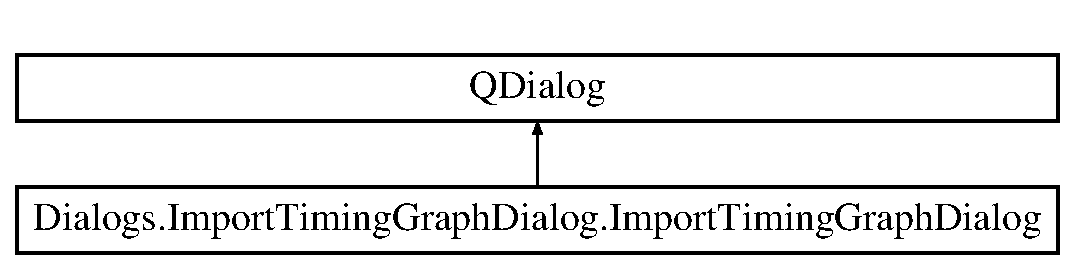
\includegraphics[height=2.000000cm]{classDialogs_1_1ImportTimingGraphDialog_1_1ImportTimingGraphDialog}
\end{center}
\end{figure}
\subsection*{Public Member Functions}
\begin{DoxyCompactItemize}
\item 
def \hyperlink{classDialogs_1_1ImportTimingGraphDialog_1_1ImportTimingGraphDialog_a851c120fd40562ddf2e19db9d86555d1}{\-\_\-\-\_\-init\-\_\-\-\_\-}
\end{DoxyCompactItemize}
\subsection*{Public Attributes}
\begin{DoxyCompactItemize}
\item 
\hypertarget{classDialogs_1_1ImportTimingGraphDialog_1_1ImportTimingGraphDialog_a6315dcc4b9b8223cd76880c35b883f20}{{\bfseries parent}}\label{classDialogs_1_1ImportTimingGraphDialog_1_1ImportTimingGraphDialog_a6315dcc4b9b8223cd76880c35b883f20}

\item 
\hypertarget{classDialogs_1_1ImportTimingGraphDialog_1_1ImportTimingGraphDialog_a94bb52491abbb58265853748a52c0f94}{{\bfseries img\-\_\-dir}}\label{classDialogs_1_1ImportTimingGraphDialog_1_1ImportTimingGraphDialog_a94bb52491abbb58265853748a52c0f94}

\item 
\hypertarget{classDialogs_1_1ImportTimingGraphDialog_1_1ImportTimingGraphDialog_a522927adb0697c9030a3a36a6b21c43a}{{\bfseries timing\-\_\-low}}\label{classDialogs_1_1ImportTimingGraphDialog_1_1ImportTimingGraphDialog_a522927adb0697c9030a3a36a6b21c43a}

\item 
\hypertarget{classDialogs_1_1ImportTimingGraphDialog_1_1ImportTimingGraphDialog_ab59f265f1bcc8f6afcab45bca08bd50f}{{\bfseries timing\-\_\-high}}\label{classDialogs_1_1ImportTimingGraphDialog_1_1ImportTimingGraphDialog_ab59f265f1bcc8f6afcab45bca08bd50f}

\item 
\hypertarget{classDialogs_1_1ImportTimingGraphDialog_1_1ImportTimingGraphDialog_ad79b95115e8feecacd7435e22ba117b3}{{\bfseries ui}}\label{classDialogs_1_1ImportTimingGraphDialog_1_1ImportTimingGraphDialog_ad79b95115e8feecacd7435e22ba117b3}

\item 
\hypertarget{classDialogs_1_1ImportTimingGraphDialog_1_1ImportTimingGraphDialog_a0de2d35c5932832c49d1f6dff2e0b122}{{\bfseries matplotlib}}\label{classDialogs_1_1ImportTimingGraphDialog_1_1ImportTimingGraphDialog_a0de2d35c5932832c49d1f6dff2e0b122}

\end{DoxyCompactItemize}


\subsection{Detailed Description}
\begin{DoxyVerb}Timing graph class for importing measurements.
\end{DoxyVerb}
 

\subsection{Constructor \& Destructor Documentation}
\hypertarget{classDialogs_1_1ImportTimingGraphDialog_1_1ImportTimingGraphDialog_a851c120fd40562ddf2e19db9d86555d1}{\index{Dialogs\-::\-Import\-Timing\-Graph\-Dialog\-::\-Import\-Timing\-Graph\-Dialog@{Dialogs\-::\-Import\-Timing\-Graph\-Dialog\-::\-Import\-Timing\-Graph\-Dialog}!\-\_\-\-\_\-init\-\_\-\-\_\-@{\-\_\-\-\_\-init\-\_\-\-\_\-}}
\index{\-\_\-\-\_\-init\-\_\-\-\_\-@{\-\_\-\-\_\-init\-\_\-\-\_\-}!Dialogs::ImportTimingGraphDialog::ImportTimingGraphDialog@{Dialogs\-::\-Import\-Timing\-Graph\-Dialog\-::\-Import\-Timing\-Graph\-Dialog}}
\subsubsection[{\-\_\-\-\_\-init\-\_\-\-\_\-}]{\setlength{\rightskip}{0pt plus 5cm}def Dialogs.\-Import\-Timing\-Graph\-Dialog.\-Import\-Timing\-Graph\-Dialog.\-\_\-\-\_\-init\-\_\-\-\_\- (
\begin{DoxyParamCaption}
\item[{}]{self, }
\item[{}]{parent, }
\item[{}]{input\-\_\-file, }
\item[{}]{output\-\_\-file, }
\item[{}]{adc\-\_\-timing\-\_\-spin, }
\item[{}]{icon\-\_\-manager, }
\item[{}]{skip\-\_\-lines, }
\item[{}]{trigger, }
\item[{}]{adc\-\_\-count, }
\item[{}]{timing, }
\item[{}]{coinc\-\_\-count}
\end{DoxyParamCaption}
)}}\label{classDialogs_1_1ImportTimingGraphDialog_1_1ImportTimingGraphDialog_a851c120fd40562ddf2e19db9d86555d1}
\begin{DoxyVerb}Inits timing graph dialog for measurement import.

Args:
    parent: An ImportMeasurementsDialog class object.
    input_file: A string representing input file.
    output_file: A string representing destination file.
    adc_timing_spin: A tuple of timing QSpinboxes.
    icon_manager: An IconManager class object.
    skip_lines: An integer representing line count to be skipped.
    trigger: An integer representing ADC number.
    adc_count: An integer representing ADC count
    timing: A dictionary of tuples for each ADC.
    coinc_count: An integer representing number of coincidences to be 
         captured from input_file.
\end{DoxyVerb}
 

The documentation for this class was generated from the following file\-:\begin{DoxyCompactItemize}
\item 
Dialogs/Import\-Timing\-Graph\-Dialog.\-py\end{DoxyCompactItemize}

\hypertarget{classModules_1_1InputValidator_1_1InputValidator}{\section{Modules.\-Input\-Validator.\-Input\-Validator Class Reference}
\label{classModules_1_1InputValidator_1_1InputValidator}\index{Modules.\-Input\-Validator.\-Input\-Validator@{Modules.\-Input\-Validator.\-Input\-Validator}}
}
Inheritance diagram for Modules.\-Input\-Validator.\-Input\-Validator\-:\begin{figure}[H]
\begin{center}
\leavevmode
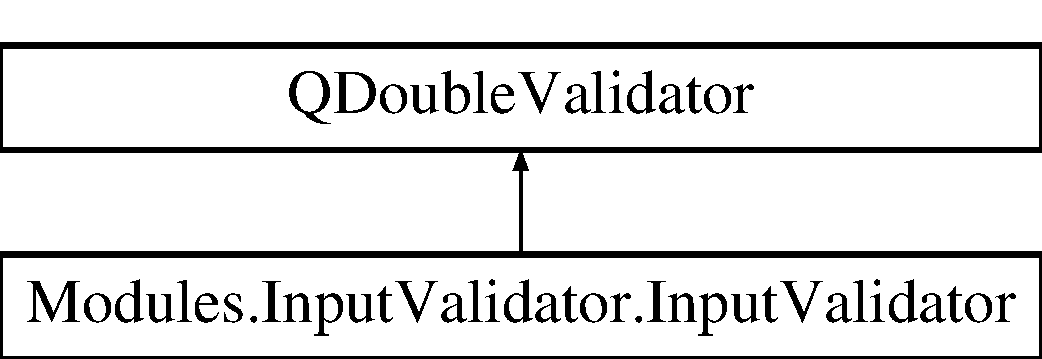
\includegraphics[height=2.000000cm]{classModules_1_1InputValidator_1_1InputValidator}
\end{center}
\end{figure}
\subsection*{Public Member Functions}
\begin{DoxyCompactItemize}
\item 
def \hyperlink{classModules_1_1InputValidator_1_1InputValidator_afd271f39a1c348c4497aafc67bab3b6f}{\-\_\-\-\_\-init\-\_\-\-\_\-}
\item 
def \hyperlink{classModules_1_1InputValidator_1_1InputValidator_ad5eeec6eb635dd74d8a892221915f065}{validate}
\end{DoxyCompactItemize}


\subsection{Detailed Description}
\begin{DoxyVerb}Validator to check the validity of user inputs.

Accepts double values with scientific notation (i.e. 0.232, 12.5e-12) and turns 
empty input to 0.0 and commas (,) to points (.).
\end{DoxyVerb}
 

\subsection{Constructor \& Destructor Documentation}
\hypertarget{classModules_1_1InputValidator_1_1InputValidator_afd271f39a1c348c4497aafc67bab3b6f}{\index{Modules\-::\-Input\-Validator\-::\-Input\-Validator@{Modules\-::\-Input\-Validator\-::\-Input\-Validator}!\-\_\-\-\_\-init\-\_\-\-\_\-@{\-\_\-\-\_\-init\-\_\-\-\_\-}}
\index{\-\_\-\-\_\-init\-\_\-\-\_\-@{\-\_\-\-\_\-init\-\_\-\-\_\-}!Modules::InputValidator::InputValidator@{Modules\-::\-Input\-Validator\-::\-Input\-Validator}}
\subsubsection[{\-\_\-\-\_\-init\-\_\-\-\_\-}]{\setlength{\rightskip}{0pt plus 5cm}def Modules.\-Input\-Validator.\-Input\-Validator.\-\_\-\-\_\-init\-\_\-\-\_\- (
\begin{DoxyParamCaption}
\item[{}]{self, }
\item[{}]{bottom = {\ttfamily float\-\_\-info.min}, }
\item[{}]{top = {\ttfamily float\-\_\-info.max}, }
\item[{}]{decimals = {\ttfamily float\-\_\-info.dig}, }
\item[{}]{parent = {\ttfamily None}}
\end{DoxyParamCaption}
)}}\label{classModules_1_1InputValidator_1_1InputValidator_afd271f39a1c348c4497aafc67bab3b6f}
\begin{DoxyVerb}Initiates the class.

Args:
    bottom: Float minimum value.
    top: Float maximum value.
    decimals: Integer representing decimals.
    parent: Parent object.
\end{DoxyVerb}
 

\subsection{Member Function Documentation}
\hypertarget{classModules_1_1InputValidator_1_1InputValidator_ad5eeec6eb635dd74d8a892221915f065}{\index{Modules\-::\-Input\-Validator\-::\-Input\-Validator@{Modules\-::\-Input\-Validator\-::\-Input\-Validator}!validate@{validate}}
\index{validate@{validate}!Modules::InputValidator::InputValidator@{Modules\-::\-Input\-Validator\-::\-Input\-Validator}}
\subsubsection[{validate}]{\setlength{\rightskip}{0pt plus 5cm}def Modules.\-Input\-Validator.\-Input\-Validator.\-validate (
\begin{DoxyParamCaption}
\item[{}]{self, }
\item[{}]{input\-\_\-value, }
\item[{}]{pos}
\end{DoxyParamCaption}
)}}\label{classModules_1_1InputValidator_1_1InputValidator_ad5eeec6eb635dd74d8a892221915f065}
\begin{DoxyVerb}Validates the given input. Overrides the QDoubleValidator's validate 
function.

Args:
    input_value: User given string to be validated.
    pos: Cursor position (if required).
\end{DoxyVerb}
 

The documentation for this class was generated from the following file\-:\begin{DoxyCompactItemize}
\item 
Modules/Input\-Validator.\-py\end{DoxyCompactItemize}

\hypertarget{classModules_1_1Element_1_1Isotope}{\section{Modules.\-Element.\-Isotope Class Reference}
\label{classModules_1_1Element_1_1Isotope}\index{Modules.\-Element.\-Isotope@{Modules.\-Element.\-Isotope}}
}
\subsection*{Public Member Functions}
\begin{DoxyCompactItemize}
\item 
def \hyperlink{classModules_1_1Element_1_1Isotope_a9c9be38415c5f2346727e61c312c2250}{\-\_\-\-\_\-init\-\_\-\-\_\-}
\item 
def \hyperlink{classModules_1_1Element_1_1Isotope_ac086b4bbea9399d108337be2f5d18b50}{\-\_\-\-\_\-str\-\_\-\-\_\-}
\end{DoxyCompactItemize}
\subsection*{Public Attributes}
\begin{DoxyCompactItemize}
\item 
\hypertarget{classModules_1_1Element_1_1Isotope_af22f299f49f7c660a235a2b980d02a5e}{{\bfseries mass}}\label{classModules_1_1Element_1_1Isotope_af22f299f49f7c660a235a2b980d02a5e}

\end{DoxyCompactItemize}


\subsection{Constructor \& Destructor Documentation}
\hypertarget{classModules_1_1Element_1_1Isotope_a9c9be38415c5f2346727e61c312c2250}{\index{Modules\-::\-Element\-::\-Isotope@{Modules\-::\-Element\-::\-Isotope}!\-\_\-\-\_\-init\-\_\-\-\_\-@{\-\_\-\-\_\-init\-\_\-\-\_\-}}
\index{\-\_\-\-\_\-init\-\_\-\-\_\-@{\-\_\-\-\_\-init\-\_\-\-\_\-}!Modules::Element::Isotope@{Modules\-::\-Element\-::\-Isotope}}
\subsubsection[{\-\_\-\-\_\-init\-\_\-\-\_\-}]{\setlength{\rightskip}{0pt plus 5cm}def Modules.\-Element.\-Isotope.\-\_\-\-\_\-init\-\_\-\-\_\- (
\begin{DoxyParamCaption}
\item[{}]{self, }
\item[{}]{isotope}
\end{DoxyParamCaption}
)}}\label{classModules_1_1Element_1_1Isotope_a9c9be38415c5f2346727e61c312c2250}
\begin{DoxyVerb}Inits isotope class.

>>> test_a = Isotope(2)
>>> test_b = Isotope("a")
Traceback (most recent call last):
...
ValueError: invalid literal for int() with base 10: 'a'
>>> print(str(test_a))
2
\end{DoxyVerb}
 

\subsection{Member Function Documentation}
\hypertarget{classModules_1_1Element_1_1Isotope_ac086b4bbea9399d108337be2f5d18b50}{\index{Modules\-::\-Element\-::\-Isotope@{Modules\-::\-Element\-::\-Isotope}!\-\_\-\-\_\-str\-\_\-\-\_\-@{\-\_\-\-\_\-str\-\_\-\-\_\-}}
\index{\-\_\-\-\_\-str\-\_\-\-\_\-@{\-\_\-\-\_\-str\-\_\-\-\_\-}!Modules::Element::Isotope@{Modules\-::\-Element\-::\-Isotope}}
\subsubsection[{\-\_\-\-\_\-str\-\_\-\-\_\-}]{\setlength{\rightskip}{0pt plus 5cm}def Modules.\-Element.\-Isotope.\-\_\-\-\_\-str\-\_\-\-\_\- (
\begin{DoxyParamCaption}
\item[{}]{self}
\end{DoxyParamCaption}
)}}\label{classModules_1_1Element_1_1Isotope_ac086b4bbea9399d108337be2f5d18b50}
\begin{DoxyVerb}Transform isotope into string.

Return:
    Returns isotope in string format.
\end{DoxyVerb}
 

The documentation for this class was generated from the following file\-:\begin{DoxyCompactItemize}
\item 
Modules/Element.\-py\end{DoxyCompactItemize}

\hypertarget{classWidgets_1_1LogWidget_1_1LogWidget}{\section{Widgets.\-Log\-Widget.\-Log\-Widget Class Reference}
\label{classWidgets_1_1LogWidget_1_1LogWidget}\index{Widgets.\-Log\-Widget.\-Log\-Widget@{Widgets.\-Log\-Widget.\-Log\-Widget}}
}
Inheritance diagram for Widgets.\-Log\-Widget.\-Log\-Widget\-:\begin{figure}[H]
\begin{center}
\leavevmode
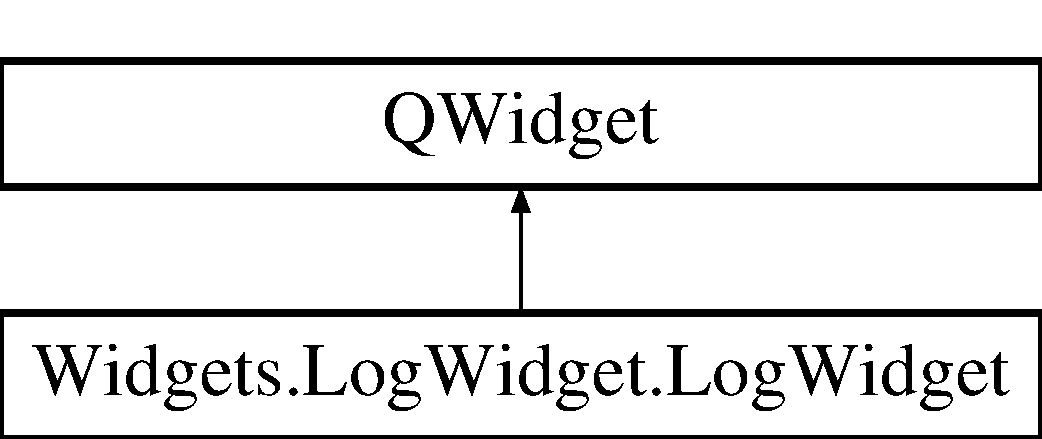
\includegraphics[height=2.000000cm]{classWidgets_1_1LogWidget_1_1LogWidget}
\end{center}
\end{figure}
\subsection*{Public Member Functions}
\begin{DoxyCompactItemize}
\item 
def \hyperlink{classWidgets_1_1LogWidget_1_1LogWidget_aa1b8db4cd22cd4cc07afbb63827c31d2}{\-\_\-\-\_\-init\-\_\-\-\_\-}
\item 
def \hyperlink{classWidgets_1_1LogWidget_1_1LogWidget_a2dbd9d8ae20f2a425a7a60dd32df1c3c}{add\-\_\-text}
\item 
def \hyperlink{classWidgets_1_1LogWidget_1_1LogWidget_a645e29634e323e67c44a0a5a9aa861f0}{add\-\_\-error}
\item 
def \hyperlink{classWidgets_1_1LogWidget_1_1LogWidget_a3b0a07e0e25fce9a0acea9efdbffcf21}{close\-Event}
\item 
def \hyperlink{classWidgets_1_1LogWidget_1_1LogWidget_a75cbcdbf6f6cba8fbc6455da1e52f922}{minimize\-\_\-window}
\end{DoxyCompactItemize}
\subsection*{Public Attributes}
\begin{DoxyCompactItemize}
\item 
\hypertarget{classWidgets_1_1LogWidget_1_1LogWidget_af3c7e4a559c5f9a41f40a69a6bc5864d}{{\bfseries want\-\_\-to\-\_\-close}}\label{classWidgets_1_1LogWidget_1_1LogWidget_af3c7e4a559c5f9a41f40a69a6bc5864d}

\item 
\hypertarget{classWidgets_1_1LogWidget_1_1LogWidget_a544043ac1e0346a04231fd07c49484bc}{{\bfseries ui}}\label{classWidgets_1_1LogWidget_1_1LogWidget_a544043ac1e0346a04231fd07c49484bc}

\end{DoxyCompactItemize}


\subsection{Detailed Description}
\begin{DoxyVerb}Log widget which displays the log. This widget handles the loghandlers emits.    
\end{DoxyVerb}
 

\subsection{Constructor \& Destructor Documentation}
\hypertarget{classWidgets_1_1LogWidget_1_1LogWidget_aa1b8db4cd22cd4cc07afbb63827c31d2}{\index{Widgets\-::\-Log\-Widget\-::\-Log\-Widget@{Widgets\-::\-Log\-Widget\-::\-Log\-Widget}!\-\_\-\-\_\-init\-\_\-\-\_\-@{\-\_\-\-\_\-init\-\_\-\-\_\-}}
\index{\-\_\-\-\_\-init\-\_\-\-\_\-@{\-\_\-\-\_\-init\-\_\-\-\_\-}!Widgets::LogWidget::LogWidget@{Widgets\-::\-Log\-Widget\-::\-Log\-Widget}}
\subsubsection[{\-\_\-\-\_\-init\-\_\-\-\_\-}]{\setlength{\rightskip}{0pt plus 5cm}def Widgets.\-Log\-Widget.\-Log\-Widget.\-\_\-\-\_\-init\-\_\-\-\_\- (
\begin{DoxyParamCaption}
\item[{}]{self}
\end{DoxyParamCaption}
)}}\label{classWidgets_1_1LogWidget_1_1LogWidget_aa1b8db4cd22cd4cc07afbb63827c31d2}
\begin{DoxyVerb}Initializes the loghandler widget.
\end{DoxyVerb}
 

\subsection{Member Function Documentation}
\hypertarget{classWidgets_1_1LogWidget_1_1LogWidget_a645e29634e323e67c44a0a5a9aa861f0}{\index{Widgets\-::\-Log\-Widget\-::\-Log\-Widget@{Widgets\-::\-Log\-Widget\-::\-Log\-Widget}!add\-\_\-error@{add\-\_\-error}}
\index{add\-\_\-error@{add\-\_\-error}!Widgets::LogWidget::LogWidget@{Widgets\-::\-Log\-Widget\-::\-Log\-Widget}}
\subsubsection[{add\-\_\-error}]{\setlength{\rightskip}{0pt plus 5cm}def Widgets.\-Log\-Widget.\-Log\-Widget.\-add\-\_\-error (
\begin{DoxyParamCaption}
\item[{}]{self, }
\item[{}]{message}
\end{DoxyParamCaption}
)}}\label{classWidgets_1_1LogWidget_1_1LogWidget_a645e29634e323e67c44a0a5a9aa861f0}
\begin{DoxyVerb}Adds the specified message to the error field.

Args:
    message: the message which will be displayed.            
\end{DoxyVerb}
 \hypertarget{classWidgets_1_1LogWidget_1_1LogWidget_a2dbd9d8ae20f2a425a7a60dd32df1c3c}{\index{Widgets\-::\-Log\-Widget\-::\-Log\-Widget@{Widgets\-::\-Log\-Widget\-::\-Log\-Widget}!add\-\_\-text@{add\-\_\-text}}
\index{add\-\_\-text@{add\-\_\-text}!Widgets::LogWidget::LogWidget@{Widgets\-::\-Log\-Widget\-::\-Log\-Widget}}
\subsubsection[{add\-\_\-text}]{\setlength{\rightskip}{0pt plus 5cm}def Widgets.\-Log\-Widget.\-Log\-Widget.\-add\-\_\-text (
\begin{DoxyParamCaption}
\item[{}]{self, }
\item[{}]{message}
\end{DoxyParamCaption}
)}}\label{classWidgets_1_1LogWidget_1_1LogWidget_a2dbd9d8ae20f2a425a7a60dd32df1c3c}
\begin{DoxyVerb}Adds the specified message to the log field.

Args:
    message: the message which will be displayed.            
\end{DoxyVerb}
 \hypertarget{classWidgets_1_1LogWidget_1_1LogWidget_a3b0a07e0e25fce9a0acea9efdbffcf21}{\index{Widgets\-::\-Log\-Widget\-::\-Log\-Widget@{Widgets\-::\-Log\-Widget\-::\-Log\-Widget}!close\-Event@{close\-Event}}
\index{close\-Event@{close\-Event}!Widgets::LogWidget::LogWidget@{Widgets\-::\-Log\-Widget\-::\-Log\-Widget}}
\subsubsection[{close\-Event}]{\setlength{\rightskip}{0pt plus 5cm}def Widgets.\-Log\-Widget.\-Log\-Widget.\-close\-Event (
\begin{DoxyParamCaption}
\item[{}]{self, }
\item[{}]{evnt}
\end{DoxyParamCaption}
)}}\label{classWidgets_1_1LogWidget_1_1LogWidget_a3b0a07e0e25fce9a0acea9efdbffcf21}
\begin{DoxyVerb}Event which happens when the windows is closing.

Instead of closing, minimize the window. This is because the disabling of
the close button isn't implemented yet. 

Args:
    envt: Close event
\end{DoxyVerb}
 \hypertarget{classWidgets_1_1LogWidget_1_1LogWidget_a75cbcdbf6f6cba8fbc6455da1e52f922}{\index{Widgets\-::\-Log\-Widget\-::\-Log\-Widget@{Widgets\-::\-Log\-Widget\-::\-Log\-Widget}!minimize\-\_\-window@{minimize\-\_\-window}}
\index{minimize\-\_\-window@{minimize\-\_\-window}!Widgets::LogWidget::LogWidget@{Widgets\-::\-Log\-Widget\-::\-Log\-Widget}}
\subsubsection[{minimize\-\_\-window}]{\setlength{\rightskip}{0pt plus 5cm}def Widgets.\-Log\-Widget.\-Log\-Widget.\-minimize\-\_\-window (
\begin{DoxyParamCaption}
\item[{}]{self}
\end{DoxyParamCaption}
)}}\label{classWidgets_1_1LogWidget_1_1LogWidget_a75cbcdbf6f6cba8fbc6455da1e52f922}
\begin{DoxyVerb}Minimize the window.
\end{DoxyVerb}
 

The documentation for this class was generated from the following file\-:\begin{DoxyCompactItemize}
\item 
Widgets/Log\-Widget.\-py\end{DoxyCompactItemize}

\hypertarget{classModules_1_1Masses_1_1Masses}{\section{Modules.\-Masses.\-Masses Class Reference}
\label{classModules_1_1Masses_1_1Masses}\index{Modules.\-Masses.\-Masses@{Modules.\-Masses.\-Masses}}
}
\subsection*{Public Member Functions}
\begin{DoxyCompactItemize}
\item 
def \hyperlink{classModules_1_1Masses_1_1Masses_afb809f124e98c55c35727b727f4f76b0}{\-\_\-\-\_\-init\-\_\-\-\_\-}
\item 
def \hyperlink{classModules_1_1Masses_1_1Masses_accc7207904ee21f66984be035036a338}{load\-\_\-isotopes}
\item 
def \hyperlink{classModules_1_1Masses_1_1Masses_a0e3a431a9468d36270a460cb1c634a5f}{get\-\_\-standard\-\_\-isotope}
\item 
def \hyperlink{classModules_1_1Masses_1_1Masses_a8ee3f00a468b3f7c3e48cfdf8b700904}{get\-\_\-most\-\_\-common\-\_\-isotope}
\end{DoxyCompactItemize}
\subsection*{Public Attributes}
\begin{DoxyCompactItemize}
\item 
\hypertarget{classModules_1_1Masses_1_1Masses_a3292673036162443cfcf8df277ea46ce}{{\bfseries isotopes}}\label{classModules_1_1Masses_1_1Masses_a3292673036162443cfcf8df277ea46ce}

\end{DoxyCompactItemize}


\subsection{Detailed Description}
\begin{DoxyVerb}Masses class handles all element isotopes' masses.
\end{DoxyVerb}
 

\subsection{Constructor \& Destructor Documentation}
\hypertarget{classModules_1_1Masses_1_1Masses_afb809f124e98c55c35727b727f4f76b0}{\index{Modules\-::\-Masses\-::\-Masses@{Modules\-::\-Masses\-::\-Masses}!\-\_\-\-\_\-init\-\_\-\-\_\-@{\-\_\-\-\_\-init\-\_\-\-\_\-}}
\index{\-\_\-\-\_\-init\-\_\-\-\_\-@{\-\_\-\-\_\-init\-\_\-\-\_\-}!Modules::Masses::Masses@{Modules\-::\-Masses\-::\-Masses}}
\subsubsection[{\-\_\-\-\_\-init\-\_\-\-\_\-}]{\setlength{\rightskip}{0pt plus 5cm}def Modules.\-Masses.\-Masses.\-\_\-\-\_\-init\-\_\-\-\_\- (
\begin{DoxyParamCaption}
\item[{}]{self, }
\item[{}]{filepath}
\end{DoxyParamCaption}
)}}\label{classModules_1_1Masses_1_1Masses_afb809f124e98c55c35727b727f4f76b0}
\begin{DoxyVerb}Inits Masses object

Args:
    filepath: String representing filepath to masses.dat
\end{DoxyVerb}
 

\subsection{Member Function Documentation}
\hypertarget{classModules_1_1Masses_1_1Masses_a8ee3f00a468b3f7c3e48cfdf8b700904}{\index{Modules\-::\-Masses\-::\-Masses@{Modules\-::\-Masses\-::\-Masses}!get\-\_\-most\-\_\-common\-\_\-isotope@{get\-\_\-most\-\_\-common\-\_\-isotope}}
\index{get\-\_\-most\-\_\-common\-\_\-isotope@{get\-\_\-most\-\_\-common\-\_\-isotope}!Modules::Masses::Masses@{Modules\-::\-Masses\-::\-Masses}}
\subsubsection[{get\-\_\-most\-\_\-common\-\_\-isotope}]{\setlength{\rightskip}{0pt plus 5cm}def Modules.\-Masses.\-Masses.\-get\-\_\-most\-\_\-common\-\_\-isotope (
\begin{DoxyParamCaption}
\item[{}]{self, }
\item[{}]{element}
\end{DoxyParamCaption}
)}}\label{classModules_1_1Masses_1_1Masses_a8ee3f00a468b3f7c3e48cfdf8b700904}
\begin{DoxyVerb}Get the most common isotope for an element.

Args:
    element: String representing element.
    
Return:
    Returns the most common isotope for the element (int)
    and the propability (commonness) of the isotope (float)
    as a tuple(int, float).
\end{DoxyVerb}
 \hypertarget{classModules_1_1Masses_1_1Masses_a0e3a431a9468d36270a460cb1c634a5f}{\index{Modules\-::\-Masses\-::\-Masses@{Modules\-::\-Masses\-::\-Masses}!get\-\_\-standard\-\_\-isotope@{get\-\_\-standard\-\_\-isotope}}
\index{get\-\_\-standard\-\_\-isotope@{get\-\_\-standard\-\_\-isotope}!Modules::Masses::Masses@{Modules\-::\-Masses\-::\-Masses}}
\subsubsection[{get\-\_\-standard\-\_\-isotope}]{\setlength{\rightskip}{0pt plus 5cm}def Modules.\-Masses.\-Masses.\-get\-\_\-standard\-\_\-isotope (
\begin{DoxyParamCaption}
\item[{}]{self, }
\item[{}]{element}
\end{DoxyParamCaption}
)}}\label{classModules_1_1Masses_1_1Masses_a0e3a431a9468d36270a460cb1c634a5f}
\begin{DoxyVerb}Calculate standard element weight.

Args:
    element: String representing element.
    
Return:
    Returns standard weight of given element (float).
\end{DoxyVerb}
 \hypertarget{classModules_1_1Masses_1_1Masses_accc7207904ee21f66984be035036a338}{\index{Modules\-::\-Masses\-::\-Masses@{Modules\-::\-Masses\-::\-Masses}!load\-\_\-isotopes@{load\-\_\-isotopes}}
\index{load\-\_\-isotopes@{load\-\_\-isotopes}!Modules::Masses::Masses@{Modules\-::\-Masses\-::\-Masses}}
\subsubsection[{load\-\_\-isotopes}]{\setlength{\rightskip}{0pt plus 5cm}def Modules.\-Masses.\-Masses.\-load\-\_\-isotopes (
\begin{DoxyParamCaption}
\item[{}]{self, }
\item[{}]{element, }
\item[{}]{combobox, }
\item[{}]{current\-\_\-isotope = {\ttfamily None}}
\end{DoxyParamCaption}
)}}\label{classModules_1_1Masses_1_1Masses_accc7207904ee21f66984be035036a338}
\begin{DoxyVerb}Load isotopes into given combobox.

Args:
    element: String representing selected element of which 
        isotopes are loaded.
    combobox: QComboBox to which items are added.
    current_isotope: Current isotope to select it on combobox by default 
             (string).
\end{DoxyVerb}
 

The documentation for this class was generated from the following file\-:\begin{DoxyCompactItemize}
\item 
Modules/Masses.\-py\end{DoxyCompactItemize}

\hypertarget{classWidgets_1_1MatplotlibCalibrationCurveFittingWidget_1_1MatplotlibCalibrationCurveFittingWidget}{\section{Widgets.\-Matplotlib\-Calibration\-Curve\-Fitting\-Widget.\-Matplotlib\-Calibration\-Curve\-Fitting\-Widget Class Reference}
\label{classWidgets_1_1MatplotlibCalibrationCurveFittingWidget_1_1MatplotlibCalibrationCurveFittingWidget}\index{Widgets.\-Matplotlib\-Calibration\-Curve\-Fitting\-Widget.\-Matplotlib\-Calibration\-Curve\-Fitting\-Widget@{Widgets.\-Matplotlib\-Calibration\-Curve\-Fitting\-Widget.\-Matplotlib\-Calibration\-Curve\-Fitting\-Widget}}
}
Inheritance diagram for Widgets.\-Matplotlib\-Calibration\-Curve\-Fitting\-Widget.\-Matplotlib\-Calibration\-Curve\-Fitting\-Widget\-:\begin{figure}[H]
\begin{center}
\leavevmode
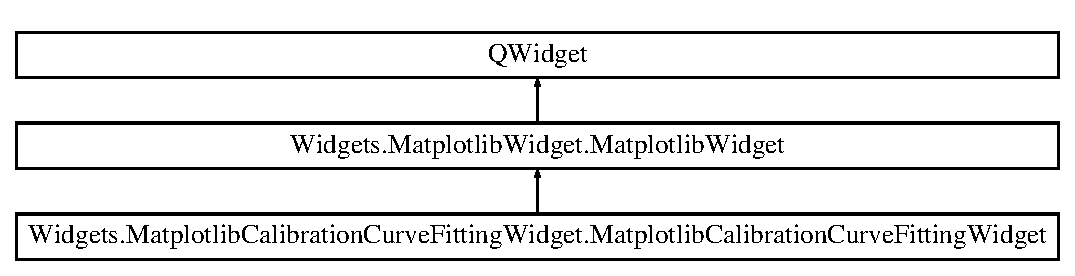
\includegraphics[height=3.000000cm]{classWidgets_1_1MatplotlibCalibrationCurveFittingWidget_1_1MatplotlibCalibrationCurveFittingWidget}
\end{center}
\end{figure}
\subsection*{Public Member Functions}
\begin{DoxyCompactItemize}
\item 
def \hyperlink{classWidgets_1_1MatplotlibCalibrationCurveFittingWidget_1_1MatplotlibCalibrationCurveFittingWidget_a61247760fbadfec08384c149b4055bba}{\-\_\-\-\_\-init\-\_\-\-\_\-}
\item 
def \hyperlink{classWidgets_1_1MatplotlibCalibrationCurveFittingWidget_1_1MatplotlibCalibrationCurveFittingWidget_a60be16b569b6aa80d08b228dd11ec886}{onclick}
\item 
def \hyperlink{classWidgets_1_1MatplotlibCalibrationCurveFittingWidget_1_1MatplotlibCalibrationCurveFittingWidget_a154426d513e47e19612c4e6750baf32c}{set\-\_\-calibration\-\_\-point\-\_\-externally}
\item 
def \hyperlink{classWidgets_1_1MatplotlibCalibrationCurveFittingWidget_1_1MatplotlibCalibrationCurveFittingWidget_ae7f878f52f776c6244b7d8eb67fafc16}{change\-\_\-cut}
\item 
def \hyperlink{classWidgets_1_1MatplotlibCalibrationCurveFittingWidget_1_1MatplotlibCalibrationCurveFittingWidget_a0d446b5d1d8a7a57df9127d1d6579ce9}{change\-\_\-bin\-\_\-width}
\item 
def \hyperlink{classWidgets_1_1MatplotlibCalibrationCurveFittingWidget_1_1MatplotlibCalibrationCurveFittingWidget_a608876b8f2dc34c35c142f5b6f2abde2}{on\-\_\-draw}
\item 
def \hyperlink{classWidgets_1_1MatplotlibCalibrationCurveFittingWidget_1_1MatplotlibCalibrationCurveFittingWidget_a4e741d993345a895a347d86a80195a91}{toggle\-\_\-clicks}
\end{DoxyCompactItemize}
\subsection*{Public Attributes}
\begin{DoxyCompactItemize}
\item 
\hypertarget{classWidgets_1_1MatplotlibCalibrationCurveFittingWidget_1_1MatplotlibCalibrationCurveFittingWidget_a055dff511b05657970b48d3f9db0bfe8}{{\bfseries dialog}}\label{classWidgets_1_1MatplotlibCalibrationCurveFittingWidget_1_1MatplotlibCalibrationCurveFittingWidget_a055dff511b05657970b48d3f9db0bfe8}

\item 
\hypertarget{classWidgets_1_1MatplotlibCalibrationCurveFittingWidget_1_1MatplotlibCalibrationCurveFittingWidget_ad7ae386a907f2dd1166cdc7092d1ef9d}{{\bfseries settings}}\label{classWidgets_1_1MatplotlibCalibrationCurveFittingWidget_1_1MatplotlibCalibrationCurveFittingWidget_ad7ae386a907f2dd1166cdc7092d1ef9d}

\item 
\hypertarget{classWidgets_1_1MatplotlibCalibrationCurveFittingWidget_1_1MatplotlibCalibrationCurveFittingWidget_a0d7fe3aec8263adfe2ef87c472f3c7fb}{{\bfseries cut}}\label{classWidgets_1_1MatplotlibCalibrationCurveFittingWidget_1_1MatplotlibCalibrationCurveFittingWidget_a0d7fe3aec8263adfe2ef87c472f3c7fb}

\item 
\hypertarget{classWidgets_1_1MatplotlibCalibrationCurveFittingWidget_1_1MatplotlibCalibrationCurveFittingWidget_a2a55773f3a5385be984a83ea32a9581c}{{\bfseries masses}}\label{classWidgets_1_1MatplotlibCalibrationCurveFittingWidget_1_1MatplotlibCalibrationCurveFittingWidget_a2a55773f3a5385be984a83ea32a9581c}

\item 
\hypertarget{classWidgets_1_1MatplotlibCalibrationCurveFittingWidget_1_1MatplotlibCalibrationCurveFittingWidget_ae481b70e75e96712298860ee1aa72210}{{\bfseries cut\-\_\-standard\-\_\-mass}}\label{classWidgets_1_1MatplotlibCalibrationCurveFittingWidget_1_1MatplotlibCalibrationCurveFittingWidget_ae481b70e75e96712298860ee1aa72210}

\item 
\hypertarget{classWidgets_1_1MatplotlibCalibrationCurveFittingWidget_1_1MatplotlibCalibrationCurveFittingWidget_af0d7627b0a9eb7501ef51343ca2d7ffa}{{\bfseries cut\-\_\-standard\-\_\-scatter\-\_\-mass}}\label{classWidgets_1_1MatplotlibCalibrationCurveFittingWidget_1_1MatplotlibCalibrationCurveFittingWidget_af0d7627b0a9eb7501ef51343ca2d7ffa}

\item 
\hypertarget{classWidgets_1_1MatplotlibCalibrationCurveFittingWidget_1_1MatplotlibCalibrationCurveFittingWidget_a23c4292d8d33f559f72830c55f4a7b15}{{\bfseries bin\-\_\-width}}\label{classWidgets_1_1MatplotlibCalibrationCurveFittingWidget_1_1MatplotlibCalibrationCurveFittingWidget_a23c4292d8d33f559f72830c55f4a7b15}

\item 
\hypertarget{classWidgets_1_1MatplotlibCalibrationCurveFittingWidget_1_1MatplotlibCalibrationCurveFittingWidget_a25742334945874913538060f99cf7338}{{\bfseries use\-\_\-column}}\label{classWidgets_1_1MatplotlibCalibrationCurveFittingWidget_1_1MatplotlibCalibrationCurveFittingWidget_a25742334945874913538060f99cf7338}

\item 
\hypertarget{classWidgets_1_1MatplotlibCalibrationCurveFittingWidget_1_1MatplotlibCalibrationCurveFittingWidget_a53fe0ef1551333cd6915ed6413e88272}{{\bfseries tof\-\_\-histogram}}\label{classWidgets_1_1MatplotlibCalibrationCurveFittingWidget_1_1MatplotlibCalibrationCurveFittingWidget_a53fe0ef1551333cd6915ed6413e88272}

\item 
\hypertarget{classWidgets_1_1MatplotlibCalibrationCurveFittingWidget_1_1MatplotlibCalibrationCurveFittingWidget_a864d5f7f5a5fb3a2b3defaf5bdb3c464}{{\bfseries tof\-\_\-calibration\-\_\-point}}\label{classWidgets_1_1MatplotlibCalibrationCurveFittingWidget_1_1MatplotlibCalibrationCurveFittingWidget_a864d5f7f5a5fb3a2b3defaf5bdb3c464}

\item 
\hypertarget{classWidgets_1_1MatplotlibCalibrationCurveFittingWidget_1_1MatplotlibCalibrationCurveFittingWidget_a7c21243b2a4c36752d3bfa5b19be311a}{{\bfseries selection\-\_\-given\-\_\-manually}}\label{classWidgets_1_1MatplotlibCalibrationCurveFittingWidget_1_1MatplotlibCalibrationCurveFittingWidget_a7c21243b2a4c36752d3bfa5b19be311a}

\item 
\hypertarget{classWidgets_1_1MatplotlibCalibrationCurveFittingWidget_1_1MatplotlibCalibrationCurveFittingWidget_add15fc8e6dfbd70eb09ab3182c243403}{{\bfseries selected\-\_\-tof}}\label{classWidgets_1_1MatplotlibCalibrationCurveFittingWidget_1_1MatplotlibCalibrationCurveFittingWidget_add15fc8e6dfbd70eb09ab3182c243403}

\item 
\hypertarget{classWidgets_1_1MatplotlibCalibrationCurveFittingWidget_1_1MatplotlibCalibrationCurveFittingWidget_a4e70488c0e34b3e43316ead650976ca0}{{\bfseries select\-Button}}\label{classWidgets_1_1MatplotlibCalibrationCurveFittingWidget_1_1MatplotlibCalibrationCurveFittingWidget_a4e70488c0e34b3e43316ead650976ca0}

\end{DoxyCompactItemize}


\subsection{Detailed Description}
\begin{DoxyVerb}Energy spectrum widget
\end{DoxyVerb}
 

\subsection{Constructor \& Destructor Documentation}
\hypertarget{classWidgets_1_1MatplotlibCalibrationCurveFittingWidget_1_1MatplotlibCalibrationCurveFittingWidget_a61247760fbadfec08384c149b4055bba}{\index{Widgets\-::\-Matplotlib\-Calibration\-Curve\-Fitting\-Widget\-::\-Matplotlib\-Calibration\-Curve\-Fitting\-Widget@{Widgets\-::\-Matplotlib\-Calibration\-Curve\-Fitting\-Widget\-::\-Matplotlib\-Calibration\-Curve\-Fitting\-Widget}!\-\_\-\-\_\-init\-\_\-\-\_\-@{\-\_\-\-\_\-init\-\_\-\-\_\-}}
\index{\-\_\-\-\_\-init\-\_\-\-\_\-@{\-\_\-\-\_\-init\-\_\-\-\_\-}!Widgets::MatplotlibCalibrationCurveFittingWidget::MatplotlibCalibrationCurveFittingWidget@{Widgets\-::\-Matplotlib\-Calibration\-Curve\-Fitting\-Widget\-::\-Matplotlib\-Calibration\-Curve\-Fitting\-Widget}}
\subsubsection[{\-\_\-\-\_\-init\-\_\-\-\_\-}]{\setlength{\rightskip}{0pt plus 5cm}def Widgets.\-Matplotlib\-Calibration\-Curve\-Fitting\-Widget.\-Matplotlib\-Calibration\-Curve\-Fitting\-Widget.\-\_\-\-\_\-init\-\_\-\-\_\- (
\begin{DoxyParamCaption}
\item[{}]{self, }
\item[{}]{parent, }
\item[{}]{settings, }
\item[{}]{tof\-\_\-calibration, }
\item[{}]{cut, }
\item[{}]{masses, }
\item[{}]{bin\-\_\-width = {\ttfamily 2.0}, }
\item[{}]{column = {\ttfamily 1}, }
\item[{}]{dialog = {\ttfamily None}}
\end{DoxyParamCaption}
)}}\label{classWidgets_1_1MatplotlibCalibrationCurveFittingWidget_1_1MatplotlibCalibrationCurveFittingWidget_a61247760fbadfec08384c149b4055bba}
\begin{DoxyVerb}Inits Energy Spectrum widget.

Args:
    parent: CalibrationCurveFittingWidget
    settings: Settings class object.
    tof_calibration: TOFCalibration class object.
    cut: CutFile class object.
    masses: Reference to element masses object of main program.
    bin_width: Histograms bin width
    column: Which column of the CutFile's data is used to create a 
    histogram.
    dialog: parent's parent dialog.
\end{DoxyVerb}
 

\subsection{Member Function Documentation}
\hypertarget{classWidgets_1_1MatplotlibCalibrationCurveFittingWidget_1_1MatplotlibCalibrationCurveFittingWidget_a0d446b5d1d8a7a57df9127d1d6579ce9}{\index{Widgets\-::\-Matplotlib\-Calibration\-Curve\-Fitting\-Widget\-::\-Matplotlib\-Calibration\-Curve\-Fitting\-Widget@{Widgets\-::\-Matplotlib\-Calibration\-Curve\-Fitting\-Widget\-::\-Matplotlib\-Calibration\-Curve\-Fitting\-Widget}!change\-\_\-bin\-\_\-width@{change\-\_\-bin\-\_\-width}}
\index{change\-\_\-bin\-\_\-width@{change\-\_\-bin\-\_\-width}!Widgets::MatplotlibCalibrationCurveFittingWidget::MatplotlibCalibrationCurveFittingWidget@{Widgets\-::\-Matplotlib\-Calibration\-Curve\-Fitting\-Widget\-::\-Matplotlib\-Calibration\-Curve\-Fitting\-Widget}}
\subsubsection[{change\-\_\-bin\-\_\-width}]{\setlength{\rightskip}{0pt plus 5cm}def Widgets.\-Matplotlib\-Calibration\-Curve\-Fitting\-Widget.\-Matplotlib\-Calibration\-Curve\-Fitting\-Widget.\-change\-\_\-bin\-\_\-width (
\begin{DoxyParamCaption}
\item[{}]{self, }
\item[{}]{bin\-\_\-width}
\end{DoxyParamCaption}
)}}\label{classWidgets_1_1MatplotlibCalibrationCurveFittingWidget_1_1MatplotlibCalibrationCurveFittingWidget_a0d446b5d1d8a7a57df9127d1d6579ce9}
\begin{DoxyVerb}Change histogram bin width.

Args:
    bin_width: Float representing graph bin width.
\end{DoxyVerb}
 \hypertarget{classWidgets_1_1MatplotlibCalibrationCurveFittingWidget_1_1MatplotlibCalibrationCurveFittingWidget_ae7f878f52f776c6244b7d8eb67fafc16}{\index{Widgets\-::\-Matplotlib\-Calibration\-Curve\-Fitting\-Widget\-::\-Matplotlib\-Calibration\-Curve\-Fitting\-Widget@{Widgets\-::\-Matplotlib\-Calibration\-Curve\-Fitting\-Widget\-::\-Matplotlib\-Calibration\-Curve\-Fitting\-Widget}!change\-\_\-cut@{change\-\_\-cut}}
\index{change\-\_\-cut@{change\-\_\-cut}!Widgets::MatplotlibCalibrationCurveFittingWidget::MatplotlibCalibrationCurveFittingWidget@{Widgets\-::\-Matplotlib\-Calibration\-Curve\-Fitting\-Widget\-::\-Matplotlib\-Calibration\-Curve\-Fitting\-Widget}}
\subsubsection[{change\-\_\-cut}]{\setlength{\rightskip}{0pt plus 5cm}def Widgets.\-Matplotlib\-Calibration\-Curve\-Fitting\-Widget.\-Matplotlib\-Calibration\-Curve\-Fitting\-Widget.\-change\-\_\-cut (
\begin{DoxyParamCaption}
\item[{}]{self, }
\item[{}]{cut}
\end{DoxyParamCaption}
)}}\label{classWidgets_1_1MatplotlibCalibrationCurveFittingWidget_1_1MatplotlibCalibrationCurveFittingWidget_ae7f878f52f776c6244b7d8eb67fafc16}
\begin{DoxyVerb}Changes the cut file to be drawn and analyzed
\end{DoxyVerb}
 \hypertarget{classWidgets_1_1MatplotlibCalibrationCurveFittingWidget_1_1MatplotlibCalibrationCurveFittingWidget_a608876b8f2dc34c35c142f5b6f2abde2}{\index{Widgets\-::\-Matplotlib\-Calibration\-Curve\-Fitting\-Widget\-::\-Matplotlib\-Calibration\-Curve\-Fitting\-Widget@{Widgets\-::\-Matplotlib\-Calibration\-Curve\-Fitting\-Widget\-::\-Matplotlib\-Calibration\-Curve\-Fitting\-Widget}!on\-\_\-draw@{on\-\_\-draw}}
\index{on\-\_\-draw@{on\-\_\-draw}!Widgets::MatplotlibCalibrationCurveFittingWidget::MatplotlibCalibrationCurveFittingWidget@{Widgets\-::\-Matplotlib\-Calibration\-Curve\-Fitting\-Widget\-::\-Matplotlib\-Calibration\-Curve\-Fitting\-Widget}}
\subsubsection[{on\-\_\-draw}]{\setlength{\rightskip}{0pt plus 5cm}def Widgets.\-Matplotlib\-Calibration\-Curve\-Fitting\-Widget.\-Matplotlib\-Calibration\-Curve\-Fitting\-Widget.\-on\-\_\-draw (
\begin{DoxyParamCaption}
\item[{}]{self}
\end{DoxyParamCaption}
)}}\label{classWidgets_1_1MatplotlibCalibrationCurveFittingWidget_1_1MatplotlibCalibrationCurveFittingWidget_a608876b8f2dc34c35c142f5b6f2abde2}
\begin{DoxyVerb}Draw method for matplotlib.
\end{DoxyVerb}
 \hypertarget{classWidgets_1_1MatplotlibCalibrationCurveFittingWidget_1_1MatplotlibCalibrationCurveFittingWidget_a60be16b569b6aa80d08b228dd11ec886}{\index{Widgets\-::\-Matplotlib\-Calibration\-Curve\-Fitting\-Widget\-::\-Matplotlib\-Calibration\-Curve\-Fitting\-Widget@{Widgets\-::\-Matplotlib\-Calibration\-Curve\-Fitting\-Widget\-::\-Matplotlib\-Calibration\-Curve\-Fitting\-Widget}!onclick@{onclick}}
\index{onclick@{onclick}!Widgets::MatplotlibCalibrationCurveFittingWidget::MatplotlibCalibrationCurveFittingWidget@{Widgets\-::\-Matplotlib\-Calibration\-Curve\-Fitting\-Widget\-::\-Matplotlib\-Calibration\-Curve\-Fitting\-Widget}}
\subsubsection[{onclick}]{\setlength{\rightskip}{0pt plus 5cm}def Widgets.\-Matplotlib\-Calibration\-Curve\-Fitting\-Widget.\-Matplotlib\-Calibration\-Curve\-Fitting\-Widget.\-onclick (
\begin{DoxyParamCaption}
\item[{}]{self, }
\item[{}]{event}
\end{DoxyParamCaption}
)}}\label{classWidgets_1_1MatplotlibCalibrationCurveFittingWidget_1_1MatplotlibCalibrationCurveFittingWidget_a60be16b569b6aa80d08b228dd11ec886}
\begin{DoxyVerb}Handles clicks on the graph

Args:
    event: Mouse click event.
\end{DoxyVerb}
 \hypertarget{classWidgets_1_1MatplotlibCalibrationCurveFittingWidget_1_1MatplotlibCalibrationCurveFittingWidget_a154426d513e47e19612c4e6750baf32c}{\index{Widgets\-::\-Matplotlib\-Calibration\-Curve\-Fitting\-Widget\-::\-Matplotlib\-Calibration\-Curve\-Fitting\-Widget@{Widgets\-::\-Matplotlib\-Calibration\-Curve\-Fitting\-Widget\-::\-Matplotlib\-Calibration\-Curve\-Fitting\-Widget}!set\-\_\-calibration\-\_\-point\-\_\-externally@{set\-\_\-calibration\-\_\-point\-\_\-externally}}
\index{set\-\_\-calibration\-\_\-point\-\_\-externally@{set\-\_\-calibration\-\_\-point\-\_\-externally}!Widgets::MatplotlibCalibrationCurveFittingWidget::MatplotlibCalibrationCurveFittingWidget@{Widgets\-::\-Matplotlib\-Calibration\-Curve\-Fitting\-Widget\-::\-Matplotlib\-Calibration\-Curve\-Fitting\-Widget}}
\subsubsection[{set\-\_\-calibration\-\_\-point\-\_\-externally}]{\setlength{\rightskip}{0pt plus 5cm}def Widgets.\-Matplotlib\-Calibration\-Curve\-Fitting\-Widget.\-Matplotlib\-Calibration\-Curve\-Fitting\-Widget.\-set\-\_\-calibration\-\_\-point\-\_\-externally (
\begin{DoxyParamCaption}
\item[{}]{self, }
\item[{}]{tof}
\end{DoxyParamCaption}
)}}\label{classWidgets_1_1MatplotlibCalibrationCurveFittingWidget_1_1MatplotlibCalibrationCurveFittingWidget_a154426d513e47e19612c4e6750baf32c}
\begin{DoxyVerb}Set calibration point.

Args:
    tof: Integer representing x axis value Time of Flight [Channel].
\end{DoxyVerb}
 \hypertarget{classWidgets_1_1MatplotlibCalibrationCurveFittingWidget_1_1MatplotlibCalibrationCurveFittingWidget_a4e741d993345a895a347d86a80195a91}{\index{Widgets\-::\-Matplotlib\-Calibration\-Curve\-Fitting\-Widget\-::\-Matplotlib\-Calibration\-Curve\-Fitting\-Widget@{Widgets\-::\-Matplotlib\-Calibration\-Curve\-Fitting\-Widget\-::\-Matplotlib\-Calibration\-Curve\-Fitting\-Widget}!toggle\-\_\-clicks@{toggle\-\_\-clicks}}
\index{toggle\-\_\-clicks@{toggle\-\_\-clicks}!Widgets::MatplotlibCalibrationCurveFittingWidget::MatplotlibCalibrationCurveFittingWidget@{Widgets\-::\-Matplotlib\-Calibration\-Curve\-Fitting\-Widget\-::\-Matplotlib\-Calibration\-Curve\-Fitting\-Widget}}
\subsubsection[{toggle\-\_\-clicks}]{\setlength{\rightskip}{0pt plus 5cm}def Widgets.\-Matplotlib\-Calibration\-Curve\-Fitting\-Widget.\-Matplotlib\-Calibration\-Curve\-Fitting\-Widget.\-toggle\-\_\-clicks (
\begin{DoxyParamCaption}
\item[{}]{self}
\end{DoxyParamCaption}
)}}\label{classWidgets_1_1MatplotlibCalibrationCurveFittingWidget_1_1MatplotlibCalibrationCurveFittingWidget_a4e741d993345a895a347d86a80195a91}
\begin{DoxyVerb}Toggle between manual ToF channel (x axis) selection.
\end{DoxyVerb}
 

The documentation for this class was generated from the following file\-:\begin{DoxyCompactItemize}
\item 
Widgets/Matplotlib\-Calibration\-Curve\-Fitting\-Widget.\-py\end{DoxyCompactItemize}

\hypertarget{classWidgets_1_1MatplotlibCalibrationLinearFittingWidget_1_1MatplotlibCalibrationLinearFittingWidget}{\section{Widgets.\-Matplotlib\-Calibration\-Linear\-Fitting\-Widget.\-Matplotlib\-Calibration\-Linear\-Fitting\-Widget Class Reference}
\label{classWidgets_1_1MatplotlibCalibrationLinearFittingWidget_1_1MatplotlibCalibrationLinearFittingWidget}\index{Widgets.\-Matplotlib\-Calibration\-Linear\-Fitting\-Widget.\-Matplotlib\-Calibration\-Linear\-Fitting\-Widget@{Widgets.\-Matplotlib\-Calibration\-Linear\-Fitting\-Widget.\-Matplotlib\-Calibration\-Linear\-Fitting\-Widget}}
}
Inheritance diagram for Widgets.\-Matplotlib\-Calibration\-Linear\-Fitting\-Widget.\-Matplotlib\-Calibration\-Linear\-Fitting\-Widget\-:\begin{figure}[H]
\begin{center}
\leavevmode
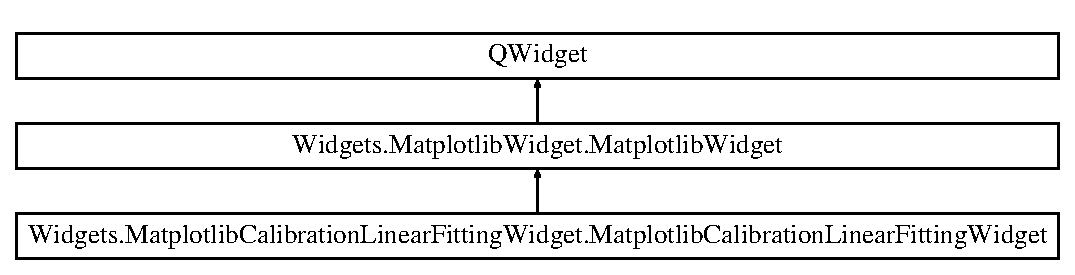
\includegraphics[height=3.000000cm]{classWidgets_1_1MatplotlibCalibrationLinearFittingWidget_1_1MatplotlibCalibrationLinearFittingWidget}
\end{center}
\end{figure}
\subsection*{Public Member Functions}
\begin{DoxyCompactItemize}
\item 
def \hyperlink{classWidgets_1_1MatplotlibCalibrationLinearFittingWidget_1_1MatplotlibCalibrationLinearFittingWidget_acd2ccb87257c23aa05ce9248cc9eada0}{\-\_\-\-\_\-init\-\_\-\-\_\-}
\item 
def \hyperlink{classWidgets_1_1MatplotlibCalibrationLinearFittingWidget_1_1MatplotlibCalibrationLinearFittingWidget_a860451c4955757770f9b291d8b35760c}{on\-\_\-draw}
\end{DoxyCompactItemize}
\subsection*{Public Attributes}
\begin{DoxyCompactItemize}
\item 
\hypertarget{classWidgets_1_1MatplotlibCalibrationLinearFittingWidget_1_1MatplotlibCalibrationLinearFittingWidget_a842eed8eb74dbcdaa40d3be2e6115ae3}{{\bfseries dialog}}\label{classWidgets_1_1MatplotlibCalibrationLinearFittingWidget_1_1MatplotlibCalibrationLinearFittingWidget_a842eed8eb74dbcdaa40d3be2e6115ae3}

\item 
\hypertarget{classWidgets_1_1MatplotlibCalibrationLinearFittingWidget_1_1MatplotlibCalibrationLinearFittingWidget_a475c744934677e1b2153b8f69f7c2755}{{\bfseries old\-\_\-params}}\label{classWidgets_1_1MatplotlibCalibrationLinearFittingWidget_1_1MatplotlibCalibrationLinearFittingWidget_a475c744934677e1b2153b8f69f7c2755}

\item 
\hypertarget{classWidgets_1_1MatplotlibCalibrationLinearFittingWidget_1_1MatplotlibCalibrationLinearFittingWidget_a4f10b3afa82c5c66d3a228a50bb20403}{{\bfseries tof\-\_\-calibration}}\label{classWidgets_1_1MatplotlibCalibrationLinearFittingWidget_1_1MatplotlibCalibrationLinearFittingWidget_a4f10b3afa82c5c66d3a228a50bb20403}

\item 
\hypertarget{classWidgets_1_1MatplotlibCalibrationLinearFittingWidget_1_1MatplotlibCalibrationLinearFittingWidget_a80b26e141899ee58ef47af310c8809d7}{{\bfseries enable\-\_\-selection\-\_\-tool}}\label{classWidgets_1_1MatplotlibCalibrationLinearFittingWidget_1_1MatplotlibCalibrationLinearFittingWidget_a80b26e141899ee58ef47af310c8809d7}

\end{DoxyCompactItemize}


\subsection{Detailed Description}
\begin{DoxyVerb}Energy spectrum widget
\end{DoxyVerb}
 

\subsection{Constructor \& Destructor Documentation}
\hypertarget{classWidgets_1_1MatplotlibCalibrationLinearFittingWidget_1_1MatplotlibCalibrationLinearFittingWidget_acd2ccb87257c23aa05ce9248cc9eada0}{\index{Widgets\-::\-Matplotlib\-Calibration\-Linear\-Fitting\-Widget\-::\-Matplotlib\-Calibration\-Linear\-Fitting\-Widget@{Widgets\-::\-Matplotlib\-Calibration\-Linear\-Fitting\-Widget\-::\-Matplotlib\-Calibration\-Linear\-Fitting\-Widget}!\-\_\-\-\_\-init\-\_\-\-\_\-@{\-\_\-\-\_\-init\-\_\-\-\_\-}}
\index{\-\_\-\-\_\-init\-\_\-\-\_\-@{\-\_\-\-\_\-init\-\_\-\-\_\-}!Widgets::MatplotlibCalibrationLinearFittingWidget::MatplotlibCalibrationLinearFittingWidget@{Widgets\-::\-Matplotlib\-Calibration\-Linear\-Fitting\-Widget\-::\-Matplotlib\-Calibration\-Linear\-Fitting\-Widget}}
\subsubsection[{\-\_\-\-\_\-init\-\_\-\-\_\-}]{\setlength{\rightskip}{0pt plus 5cm}def Widgets.\-Matplotlib\-Calibration\-Linear\-Fitting\-Widget.\-Matplotlib\-Calibration\-Linear\-Fitting\-Widget.\-\_\-\-\_\-init\-\_\-\-\_\- (
\begin{DoxyParamCaption}
\item[{}]{self, }
\item[{}]{parent, }
\item[{}]{tof\-\_\-calibration, }
\item[{}]{dialog = {\ttfamily None}, }
\item[{}]{old\-\_\-params = {\ttfamily None}}
\end{DoxyParamCaption}
)}}\label{classWidgets_1_1MatplotlibCalibrationLinearFittingWidget_1_1MatplotlibCalibrationLinearFittingWidget_acd2ccb87257c23aa05ce9248cc9eada0}
\begin{DoxyVerb}Inits Energy Spectrum widget.

Args:
    parent: CalibrationCurveFittingWidget
    tof_calibration: TOFCalibration class object.
    dialog: parent's parent dialog.
    old_params: tuple of parameters (x0, A, k)
\end{DoxyVerb}
 

\subsection{Member Function Documentation}
\hypertarget{classWidgets_1_1MatplotlibCalibrationLinearFittingWidget_1_1MatplotlibCalibrationLinearFittingWidget_a860451c4955757770f9b291d8b35760c}{\index{Widgets\-::\-Matplotlib\-Calibration\-Linear\-Fitting\-Widget\-::\-Matplotlib\-Calibration\-Linear\-Fitting\-Widget@{Widgets\-::\-Matplotlib\-Calibration\-Linear\-Fitting\-Widget\-::\-Matplotlib\-Calibration\-Linear\-Fitting\-Widget}!on\-\_\-draw@{on\-\_\-draw}}
\index{on\-\_\-draw@{on\-\_\-draw}!Widgets::MatplotlibCalibrationLinearFittingWidget::MatplotlibCalibrationLinearFittingWidget@{Widgets\-::\-Matplotlib\-Calibration\-Linear\-Fitting\-Widget\-::\-Matplotlib\-Calibration\-Linear\-Fitting\-Widget}}
\subsubsection[{on\-\_\-draw}]{\setlength{\rightskip}{0pt plus 5cm}def Widgets.\-Matplotlib\-Calibration\-Linear\-Fitting\-Widget.\-Matplotlib\-Calibration\-Linear\-Fitting\-Widget.\-on\-\_\-draw (
\begin{DoxyParamCaption}
\item[{}]{self}
\end{DoxyParamCaption}
)}}\label{classWidgets_1_1MatplotlibCalibrationLinearFittingWidget_1_1MatplotlibCalibrationLinearFittingWidget_a860451c4955757770f9b291d8b35760c}
\begin{DoxyVerb}Draw method for matplotlib.
\end{DoxyVerb}
 

The documentation for this class was generated from the following file\-:\begin{DoxyCompactItemize}
\item 
Widgets/Matplotlib\-Calibration\-Linear\-Fitting\-Widget.\-py\end{DoxyCompactItemize}

\hypertarget{classWidgets_1_1MatplotlibDepthProfileWidget_1_1MatplotlibDepthProfileWidget}{\section{Widgets.\-Matplotlib\-Depth\-Profile\-Widget.\-Matplotlib\-Depth\-Profile\-Widget Class Reference}
\label{classWidgets_1_1MatplotlibDepthProfileWidget_1_1MatplotlibDepthProfileWidget}\index{Widgets.\-Matplotlib\-Depth\-Profile\-Widget.\-Matplotlib\-Depth\-Profile\-Widget@{Widgets.\-Matplotlib\-Depth\-Profile\-Widget.\-Matplotlib\-Depth\-Profile\-Widget}}
}
Inheritance diagram for Widgets.\-Matplotlib\-Depth\-Profile\-Widget.\-Matplotlib\-Depth\-Profile\-Widget\-:\begin{figure}[H]
\begin{center}
\leavevmode
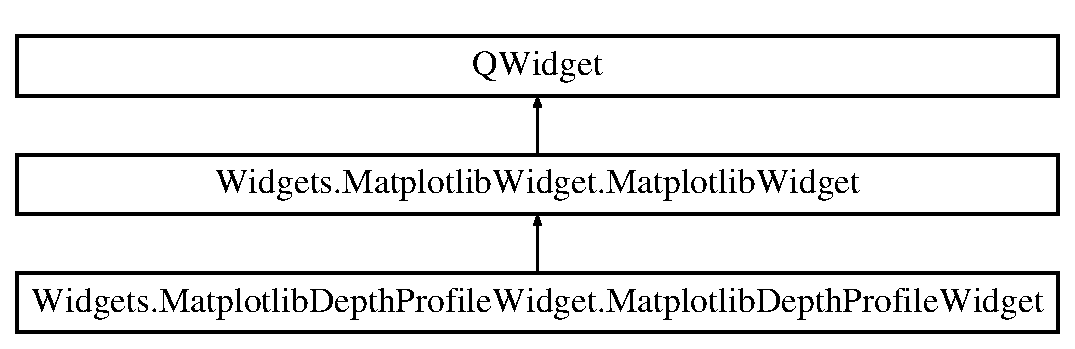
\includegraphics[height=3.000000cm]{classWidgets_1_1MatplotlibDepthProfileWidget_1_1MatplotlibDepthProfileWidget}
\end{center}
\end{figure}
\subsection*{Classes}
\begin{DoxyCompactItemize}
\item 
class \hyperlink{classWidgets_1_1MatplotlibDepthProfileWidget_1_1MatplotlibDepthProfileWidget_1_1____limit}{\-\_\-\-\_\-limit}
\end{DoxyCompactItemize}
\subsection*{Public Member Functions}
\begin{DoxyCompactItemize}
\item 
def \hyperlink{classWidgets_1_1MatplotlibDepthProfileWidget_1_1MatplotlibDepthProfileWidget_a8cdd8394cfdb9827714c562f754d6a2d}{\-\_\-\-\_\-init\-\_\-\-\_\-}
\item 
def \hyperlink{classWidgets_1_1MatplotlibDepthProfileWidget_1_1MatplotlibDepthProfileWidget_abb09afd7aabf9bd23c66781f95cf8e6d}{onclick}
\item 
def \hyperlink{classWidgets_1_1MatplotlibDepthProfileWidget_1_1MatplotlibDepthProfileWidget_a1c417e9a539e8c97c0bc897d45570edc}{on\-\_\-draw}
\end{DoxyCompactItemize}
\subsection*{Public Attributes}
\begin{DoxyCompactItemize}
\item 
\hypertarget{classWidgets_1_1MatplotlibDepthProfileWidget_1_1MatplotlibDepthProfileWidget_ab98e5fc6ef0d3bf653530728d3bfafab}{{\bfseries x\-\_\-units}}\label{classWidgets_1_1MatplotlibDepthProfileWidget_1_1MatplotlibDepthProfileWidget_ab98e5fc6ef0d3bf653530728d3bfafab}

\item 
\hypertarget{classWidgets_1_1MatplotlibDepthProfileWidget_1_1MatplotlibDepthProfileWidget_a1454f115abe2f4a7103e7c1af944a2e8}{{\bfseries draw\-\_\-legend}}\label{classWidgets_1_1MatplotlibDepthProfileWidget_1_1MatplotlibDepthProfileWidget_a1454f115abe2f4a7103e7c1af944a2e8}

\item 
\hypertarget{classWidgets_1_1MatplotlibDepthProfileWidget_1_1MatplotlibDepthProfileWidget_ab7be60c8dfffbf2c1062ff07b870898a}{{\bfseries elements}}\label{classWidgets_1_1MatplotlibDepthProfileWidget_1_1MatplotlibDepthProfileWidget_ab7be60c8dfffbf2c1062ff07b870898a}

\item 
\hypertarget{classWidgets_1_1MatplotlibDepthProfileWidget_1_1MatplotlibDepthProfileWidget_a0bfc94b324477f8ae44e9618bd78a1ad}{{\bfseries depth\-\_\-dir}}\label{classWidgets_1_1MatplotlibDepthProfileWidget_1_1MatplotlibDepthProfileWidget_a0bfc94b324477f8ae44e9618bd78a1ad}

\item 
\hypertarget{classWidgets_1_1MatplotlibDepthProfileWidget_1_1MatplotlibDepthProfileWidget_aaf8ec349976d262b2bea2f3ae9292aa4}{{\bfseries depth\-\_\-files}}\label{classWidgets_1_1MatplotlibDepthProfileWidget_1_1MatplotlibDepthProfileWidget_aaf8ec349976d262b2bea2f3ae9292aa4}

\item 
\hypertarget{classWidgets_1_1MatplotlibDepthProfileWidget_1_1MatplotlibDepthProfileWidget_abdb846768c7b58e752afafa97efdb193}{{\bfseries read\-\_\-files}}\label{classWidgets_1_1MatplotlibDepthProfileWidget_1_1MatplotlibDepthProfileWidget_abdb846768c7b58e752afafa97efdb193}

\item 
\hypertarget{classWidgets_1_1MatplotlibDepthProfileWidget_1_1MatplotlibDepthProfileWidget_ae3b5414a3f9f58872136bacfb5dbd6ae}{{\bfseries rel\-\_\-files}}\label{classWidgets_1_1MatplotlibDepthProfileWidget_1_1MatplotlibDepthProfileWidget_ae3b5414a3f9f58872136bacfb5dbd6ae}

\item 
\hypertarget{classWidgets_1_1MatplotlibDepthProfileWidget_1_1MatplotlibDepthProfileWidget_af87ab2d2337fa8c5b9fd941e9eb8388e}{{\bfseries hyb\-\_\-files}}\label{classWidgets_1_1MatplotlibDepthProfileWidget_1_1MatplotlibDepthProfileWidget_af87ab2d2337fa8c5b9fd941e9eb8388e}

\item 
\hypertarget{classWidgets_1_1MatplotlibDepthProfileWidget_1_1MatplotlibDepthProfileWidget_a9d43c6f2d5a00df6f22494111f1d3826}{{\bfseries selection\-\_\-colors}}\label{classWidgets_1_1MatplotlibDepthProfileWidget_1_1MatplotlibDepthProfileWidget_a9d43c6f2d5a00df6f22494111f1d3826}

\item 
\hypertarget{classWidgets_1_1MatplotlibDepthProfileWidget_1_1MatplotlibDepthProfileWidget_afed257512a69dc85e94db0807dcced29}{{\bfseries icon\-\_\-manager}}\label{classWidgets_1_1MatplotlibDepthProfileWidget_1_1MatplotlibDepthProfileWidget_afed257512a69dc85e94db0807dcced29}

\item 
\hypertarget{classWidgets_1_1MatplotlibDepthProfileWidget_1_1MatplotlibDepthProfileWidget_a700bf16e1f46d02d7964f38379b18ced}{{\bfseries lim\-\_\-a}}\label{classWidgets_1_1MatplotlibDepthProfileWidget_1_1MatplotlibDepthProfileWidget_a700bf16e1f46d02d7964f38379b18ced}

\item 
\hypertarget{classWidgets_1_1MatplotlibDepthProfileWidget_1_1MatplotlibDepthProfileWidget_a61a61eea4a77c031b280744756ba7032}{{\bfseries lim\-\_\-b}}\label{classWidgets_1_1MatplotlibDepthProfileWidget_1_1MatplotlibDepthProfileWidget_a61a61eea4a77c031b280744756ba7032}

\item 
\hypertarget{classWidgets_1_1MatplotlibDepthProfileWidget_1_1MatplotlibDepthProfileWidget_a1997611147238c5a746f578201456de6}{{\bfseries lim\-\_\-icons}}\label{classWidgets_1_1MatplotlibDepthProfileWidget_1_1MatplotlibDepthProfileWidget_a1997611147238c5a746f578201456de6}

\item 
\hypertarget{classWidgets_1_1MatplotlibDepthProfileWidget_1_1MatplotlibDepthProfileWidget_ae7c7521868086c488fae83ad886ee6ec}{{\bfseries lim\-\_\-mode}}\label{classWidgets_1_1MatplotlibDepthProfileWidget_1_1MatplotlibDepthProfileWidget_ae7c7521868086c488fae83ad886ee6ec}

\item 
\hypertarget{classWidgets_1_1MatplotlibDepthProfileWidget_1_1MatplotlibDepthProfileWidget_aea7a81640fb4cbc279f4eb9a7cc390ba}{{\bfseries lim\-Button}}\label{classWidgets_1_1MatplotlibDepthProfileWidget_1_1MatplotlibDepthProfileWidget_aea7a81640fb4cbc279f4eb9a7cc390ba}

\item 
\hypertarget{classWidgets_1_1MatplotlibDepthProfileWidget_1_1MatplotlibDepthProfileWidget_a4232f90b49710bf0e85c053d96b29665}{{\bfseries mode\-Button}}\label{classWidgets_1_1MatplotlibDepthProfileWidget_1_1MatplotlibDepthProfileWidget_a4232f90b49710bf0e85c053d96b29665}

\item 
\hypertarget{classWidgets_1_1MatplotlibDepthProfileWidget_1_1MatplotlibDepthProfileWidget_a1ed4302554a0c3a461fd94c4110ea094}{{\bfseries view\-Button}}\label{classWidgets_1_1MatplotlibDepthProfileWidget_1_1MatplotlibDepthProfileWidget_a1ed4302554a0c3a461fd94c4110ea094}

\end{DoxyCompactItemize}


\subsection{Detailed Description}
\begin{DoxyVerb}Depth profile widget.
\end{DoxyVerb}
 

\subsection{Constructor \& Destructor Documentation}
\hypertarget{classWidgets_1_1MatplotlibDepthProfileWidget_1_1MatplotlibDepthProfileWidget_a8cdd8394cfdb9827714c562f754d6a2d}{\index{Widgets\-::\-Matplotlib\-Depth\-Profile\-Widget\-::\-Matplotlib\-Depth\-Profile\-Widget@{Widgets\-::\-Matplotlib\-Depth\-Profile\-Widget\-::\-Matplotlib\-Depth\-Profile\-Widget}!\-\_\-\-\_\-init\-\_\-\-\_\-@{\-\_\-\-\_\-init\-\_\-\-\_\-}}
\index{\-\_\-\-\_\-init\-\_\-\-\_\-@{\-\_\-\-\_\-init\-\_\-\-\_\-}!Widgets::MatplotlibDepthProfileWidget::MatplotlibDepthProfileWidget@{Widgets\-::\-Matplotlib\-Depth\-Profile\-Widget\-::\-Matplotlib\-Depth\-Profile\-Widget}}
\subsubsection[{\-\_\-\-\_\-init\-\_\-\-\_\-}]{\setlength{\rightskip}{0pt plus 5cm}def Widgets.\-Matplotlib\-Depth\-Profile\-Widget.\-Matplotlib\-Depth\-Profile\-Widget.\-\_\-\-\_\-init\-\_\-\-\_\- (
\begin{DoxyParamCaption}
\item[{}]{self, }
\item[{}]{parent, }
\item[{}]{depth\-\_\-dir, }
\item[{}]{elements, }
\item[{}]{rbs\-\_\-list, }
\item[{}]{depth\-\_\-scale, }
\item[{}]{x\-\_\-units = {\ttfamily 'nm'}, }
\item[{}]{legend = {\ttfamily True}, }
\item[{}]{line\-\_\-zero = {\ttfamily False}, }
\item[{}]{line\-\_\-scale = {\ttfamily False}, }
\item[{}]{systematic\-\_\-error = {\ttfamily 3.0}}
\end{DoxyParamCaption}
)}}\label{classWidgets_1_1MatplotlibDepthProfileWidget_1_1MatplotlibDepthProfileWidget_a8cdd8394cfdb9827714c562f754d6a2d}
\begin{DoxyVerb}Inits depth profile widget.

Args:
    parent: A DepthProfileWidget class object.
    depth_dir: A directory where the depth files are located.
    elements: A list of Element objects.
    rbs_list: A dictionary of RBS selection elements containing 
      scatter elements.
    depth_scale: A tuple of depth scaling values.
    x_units: An unit to be used as x axis.
    legend: A boolean of whether to show the legend.
    line_zero: A boolean representing if vertical line is drawn at zero.
    line_scale: A boolean representing if horizontal line is drawn at 
        the defined depth scale.
    systematic_error: A double representing systematic error.
\end{DoxyVerb}
 

\subsection{Member Function Documentation}
\hypertarget{classWidgets_1_1MatplotlibDepthProfileWidget_1_1MatplotlibDepthProfileWidget_a1c417e9a539e8c97c0bc897d45570edc}{\index{Widgets\-::\-Matplotlib\-Depth\-Profile\-Widget\-::\-Matplotlib\-Depth\-Profile\-Widget@{Widgets\-::\-Matplotlib\-Depth\-Profile\-Widget\-::\-Matplotlib\-Depth\-Profile\-Widget}!on\-\_\-draw@{on\-\_\-draw}}
\index{on\-\_\-draw@{on\-\_\-draw}!Widgets::MatplotlibDepthProfileWidget::MatplotlibDepthProfileWidget@{Widgets\-::\-Matplotlib\-Depth\-Profile\-Widget\-::\-Matplotlib\-Depth\-Profile\-Widget}}
\subsubsection[{on\-\_\-draw}]{\setlength{\rightskip}{0pt plus 5cm}def Widgets.\-Matplotlib\-Depth\-Profile\-Widget.\-Matplotlib\-Depth\-Profile\-Widget.\-on\-\_\-draw (
\begin{DoxyParamCaption}
\item[{}]{self}
\end{DoxyParamCaption}
)}}\label{classWidgets_1_1MatplotlibDepthProfileWidget_1_1MatplotlibDepthProfileWidget_a1c417e9a539e8c97c0bc897d45570edc}
\begin{DoxyVerb}Draws the depth profile graph
\end{DoxyVerb}
 \hypertarget{classWidgets_1_1MatplotlibDepthProfileWidget_1_1MatplotlibDepthProfileWidget_abb09afd7aabf9bd23c66781f95cf8e6d}{\index{Widgets\-::\-Matplotlib\-Depth\-Profile\-Widget\-::\-Matplotlib\-Depth\-Profile\-Widget@{Widgets\-::\-Matplotlib\-Depth\-Profile\-Widget\-::\-Matplotlib\-Depth\-Profile\-Widget}!onclick@{onclick}}
\index{onclick@{onclick}!Widgets::MatplotlibDepthProfileWidget::MatplotlibDepthProfileWidget@{Widgets\-::\-Matplotlib\-Depth\-Profile\-Widget\-::\-Matplotlib\-Depth\-Profile\-Widget}}
\subsubsection[{onclick}]{\setlength{\rightskip}{0pt plus 5cm}def Widgets.\-Matplotlib\-Depth\-Profile\-Widget.\-Matplotlib\-Depth\-Profile\-Widget.\-onclick (
\begin{DoxyParamCaption}
\item[{}]{self, }
\item[{}]{event}
\end{DoxyParamCaption}
)}}\label{classWidgets_1_1MatplotlibDepthProfileWidget_1_1MatplotlibDepthProfileWidget_abb09afd7aabf9bd23c66781f95cf8e6d}
\begin{DoxyVerb}Handles clicks on the graph.

Args:
    event: A click event on the graph
\end{DoxyVerb}
 

The documentation for this class was generated from the following file\-:\begin{DoxyCompactItemize}
\item 
Widgets/Matplotlib\-Depth\-Profile\-Widget.\-py\end{DoxyCompactItemize}

\hypertarget{classWidgets_1_1MatplotlibElementLossesWidget_1_1MatplotlibElementLossesWidget}{\section{Widgets.\-Matplotlib\-Element\-Losses\-Widget.\-Matplotlib\-Element\-Losses\-Widget Class Reference}
\label{classWidgets_1_1MatplotlibElementLossesWidget_1_1MatplotlibElementLossesWidget}\index{Widgets.\-Matplotlib\-Element\-Losses\-Widget.\-Matplotlib\-Element\-Losses\-Widget@{Widgets.\-Matplotlib\-Element\-Losses\-Widget.\-Matplotlib\-Element\-Losses\-Widget}}
}
Inheritance diagram for Widgets.\-Matplotlib\-Element\-Losses\-Widget.\-Matplotlib\-Element\-Losses\-Widget\-:\begin{figure}[H]
\begin{center}
\leavevmode
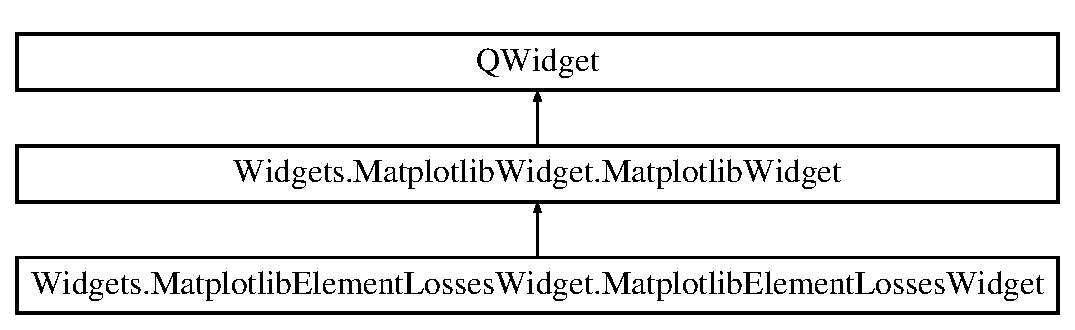
\includegraphics[height=3.000000cm]{classWidgets_1_1MatplotlibElementLossesWidget_1_1MatplotlibElementLossesWidget}
\end{center}
\end{figure}
\subsection*{Public Member Functions}
\begin{DoxyCompactItemize}
\item 
def \hyperlink{classWidgets_1_1MatplotlibElementLossesWidget_1_1MatplotlibElementLossesWidget_a6a11ddff80e87bdffe8755af53f8479d}{\-\_\-\-\_\-init\-\_\-\-\_\-}
\item 
def \hyperlink{classWidgets_1_1MatplotlibElementLossesWidget_1_1MatplotlibElementLossesWidget_a327fc01d1a404206f753fbef144f8518}{on\-\_\-draw}
\end{DoxyCompactItemize}
\subsection*{Public Attributes}
\begin{DoxyCompactItemize}
\item 
\hypertarget{classWidgets_1_1MatplotlibElementLossesWidget_1_1MatplotlibElementLossesWidget_a1495ff5fb283999f559d558398be2a7e}{{\bfseries draw\-\_\-legend}}\label{classWidgets_1_1MatplotlibElementLossesWidget_1_1MatplotlibElementLossesWidget_a1495ff5fb283999f559d558398be2a7e}

\item 
\hypertarget{classWidgets_1_1MatplotlibElementLossesWidget_1_1MatplotlibElementLossesWidget_aa06fb09c65501b47d55ecba0b2be78ec}{{\bfseries split}}\label{classWidgets_1_1MatplotlibElementLossesWidget_1_1MatplotlibElementLossesWidget_aa06fb09c65501b47d55ecba0b2be78ec}

\item 
\hypertarget{classWidgets_1_1MatplotlibElementLossesWidget_1_1MatplotlibElementLossesWidget_a92a126af64e60b420ee35416c4337b18}{{\bfseries y\-\_\-scale}}\label{classWidgets_1_1MatplotlibElementLossesWidget_1_1MatplotlibElementLossesWidget_a92a126af64e60b420ee35416c4337b18}

\item 
\hypertarget{classWidgets_1_1MatplotlibElementLossesWidget_1_1MatplotlibElementLossesWidget_a289770e2727e446a7ccb7c9062e4f233}{{\bfseries selection\-\_\-colors}}\label{classWidgets_1_1MatplotlibElementLossesWidget_1_1MatplotlibElementLossesWidget_a289770e2727e446a7ccb7c9062e4f233}

\end{DoxyCompactItemize}


\subsection{Detailed Description}
\begin{DoxyVerb}Energy spectrum widget
\end{DoxyVerb}
 

\subsection{Constructor \& Destructor Documentation}
\hypertarget{classWidgets_1_1MatplotlibElementLossesWidget_1_1MatplotlibElementLossesWidget_a6a11ddff80e87bdffe8755af53f8479d}{\index{Widgets\-::\-Matplotlib\-Element\-Losses\-Widget\-::\-Matplotlib\-Element\-Losses\-Widget@{Widgets\-::\-Matplotlib\-Element\-Losses\-Widget\-::\-Matplotlib\-Element\-Losses\-Widget}!\-\_\-\-\_\-init\-\_\-\-\_\-@{\-\_\-\-\_\-init\-\_\-\-\_\-}}
\index{\-\_\-\-\_\-init\-\_\-\-\_\-@{\-\_\-\-\_\-init\-\_\-\-\_\-}!Widgets::MatplotlibElementLossesWidget::MatplotlibElementLossesWidget@{Widgets\-::\-Matplotlib\-Element\-Losses\-Widget\-::\-Matplotlib\-Element\-Losses\-Widget}}
\subsubsection[{\-\_\-\-\_\-init\-\_\-\-\_\-}]{\setlength{\rightskip}{0pt plus 5cm}def Widgets.\-Matplotlib\-Element\-Losses\-Widget.\-Matplotlib\-Element\-Losses\-Widget.\-\_\-\-\_\-init\-\_\-\-\_\- (
\begin{DoxyParamCaption}
\item[{}]{self, }
\item[{}]{parent, }
\item[{}]{split, }
\item[{}]{legend = {\ttfamily True}, }
\item[{}]{y\-\_\-scale = {\ttfamily 0}, }
\item[{}]{rbs\-\_\-list = {\ttfamily \{\}}}
\end{DoxyParamCaption}
)}}\label{classWidgets_1_1MatplotlibElementLossesWidget_1_1MatplotlibElementLossesWidget_a6a11ddff80e87bdffe8755af53f8479d}
\begin{DoxyVerb}Inits Energy Spectrum widget.

Args:
    parent: An ElementLossesWidget class object.
    split: A list of counted split counts for each element.
    legend: A boolean representing whether to draw legend or not.
    y_scale: An integer flag representing Y axis scaling mode.
    rbs_list: A dictionary of RBS selection elements containing 
      scatter elements.
\end{DoxyVerb}
 

\subsection{Member Function Documentation}
\hypertarget{classWidgets_1_1MatplotlibElementLossesWidget_1_1MatplotlibElementLossesWidget_a327fc01d1a404206f753fbef144f8518}{\index{Widgets\-::\-Matplotlib\-Element\-Losses\-Widget\-::\-Matplotlib\-Element\-Losses\-Widget@{Widgets\-::\-Matplotlib\-Element\-Losses\-Widget\-::\-Matplotlib\-Element\-Losses\-Widget}!on\-\_\-draw@{on\-\_\-draw}}
\index{on\-\_\-draw@{on\-\_\-draw}!Widgets::MatplotlibElementLossesWidget::MatplotlibElementLossesWidget@{Widgets\-::\-Matplotlib\-Element\-Losses\-Widget\-::\-Matplotlib\-Element\-Losses\-Widget}}
\subsubsection[{on\-\_\-draw}]{\setlength{\rightskip}{0pt plus 5cm}def Widgets.\-Matplotlib\-Element\-Losses\-Widget.\-Matplotlib\-Element\-Losses\-Widget.\-on\-\_\-draw (
\begin{DoxyParamCaption}
\item[{}]{self}
\end{DoxyParamCaption}
)}}\label{classWidgets_1_1MatplotlibElementLossesWidget_1_1MatplotlibElementLossesWidget_a327fc01d1a404206f753fbef144f8518}
\begin{DoxyVerb}Draw method for matplotlib.
\end{DoxyVerb}
 

The documentation for this class was generated from the following file\-:\begin{DoxyCompactItemize}
\item 
Widgets/Matplotlib\-Element\-Losses\-Widget.\-py\end{DoxyCompactItemize}

\hypertarget{classWidgets_1_1MatplotlibEnergySpectrumWidget_1_1MatplotlibEnergySpectrumWidget}{\section{Widgets.\-Matplotlib\-Energy\-Spectrum\-Widget.\-Matplotlib\-Energy\-Spectrum\-Widget Class Reference}
\label{classWidgets_1_1MatplotlibEnergySpectrumWidget_1_1MatplotlibEnergySpectrumWidget}\index{Widgets.\-Matplotlib\-Energy\-Spectrum\-Widget.\-Matplotlib\-Energy\-Spectrum\-Widget@{Widgets.\-Matplotlib\-Energy\-Spectrum\-Widget.\-Matplotlib\-Energy\-Spectrum\-Widget}}
}
Inheritance diagram for Widgets.\-Matplotlib\-Energy\-Spectrum\-Widget.\-Matplotlib\-Energy\-Spectrum\-Widget\-:\begin{figure}[H]
\begin{center}
\leavevmode
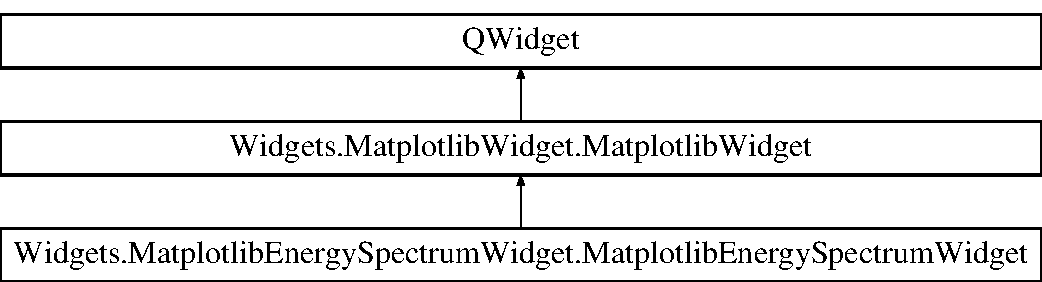
\includegraphics[height=3.000000cm]{classWidgets_1_1MatplotlibEnergySpectrumWidget_1_1MatplotlibEnergySpectrumWidget}
\end{center}
\end{figure}
\subsection*{Public Member Functions}
\begin{DoxyCompactItemize}
\item 
def \hyperlink{classWidgets_1_1MatplotlibEnergySpectrumWidget_1_1MatplotlibEnergySpectrumWidget_a311b6797d20e3a09541dade43ec451dd}{\-\_\-\-\_\-init\-\_\-\-\_\-}
\item 
def \hyperlink{classWidgets_1_1MatplotlibEnergySpectrumWidget_1_1MatplotlibEnergySpectrumWidget_a4f9443abd209aafb45e790e6cb4c4e73}{on\-\_\-draw}
\end{DoxyCompactItemize}
\subsection*{Public Attributes}
\begin{DoxyCompactItemize}
\item 
\hypertarget{classWidgets_1_1MatplotlibEnergySpectrumWidget_1_1MatplotlibEnergySpectrumWidget_a1e747851d4852985bc8c6c719a7e61d4}{{\bfseries draw\-\_\-legend}}\label{classWidgets_1_1MatplotlibEnergySpectrumWidget_1_1MatplotlibEnergySpectrumWidget_a1e747851d4852985bc8c6c719a7e61d4}

\item 
\hypertarget{classWidgets_1_1MatplotlibEnergySpectrumWidget_1_1MatplotlibEnergySpectrumWidget_a4f68106982addccb44d6d79d0078d065}{{\bfseries histed\-\_\-files}}\label{classWidgets_1_1MatplotlibEnergySpectrumWidget_1_1MatplotlibEnergySpectrumWidget_a4f68106982addccb44d6d79d0078d065}

\end{DoxyCompactItemize}


\subsection{Detailed Description}
\begin{DoxyVerb}Energy spectrum widget
\end{DoxyVerb}
 

\subsection{Constructor \& Destructor Documentation}
\hypertarget{classWidgets_1_1MatplotlibEnergySpectrumWidget_1_1MatplotlibEnergySpectrumWidget_a311b6797d20e3a09541dade43ec451dd}{\index{Widgets\-::\-Matplotlib\-Energy\-Spectrum\-Widget\-::\-Matplotlib\-Energy\-Spectrum\-Widget@{Widgets\-::\-Matplotlib\-Energy\-Spectrum\-Widget\-::\-Matplotlib\-Energy\-Spectrum\-Widget}!\-\_\-\-\_\-init\-\_\-\-\_\-@{\-\_\-\-\_\-init\-\_\-\-\_\-}}
\index{\-\_\-\-\_\-init\-\_\-\-\_\-@{\-\_\-\-\_\-init\-\_\-\-\_\-}!Widgets::MatplotlibEnergySpectrumWidget::MatplotlibEnergySpectrumWidget@{Widgets\-::\-Matplotlib\-Energy\-Spectrum\-Widget\-::\-Matplotlib\-Energy\-Spectrum\-Widget}}
\subsubsection[{\-\_\-\-\_\-init\-\_\-\-\_\-}]{\setlength{\rightskip}{0pt plus 5cm}def Widgets.\-Matplotlib\-Energy\-Spectrum\-Widget.\-Matplotlib\-Energy\-Spectrum\-Widget.\-\_\-\-\_\-init\-\_\-\-\_\- (
\begin{DoxyParamCaption}
\item[{}]{self, }
\item[{}]{parent, }
\item[{}]{histed\-\_\-files, }
\item[{}]{rbs\-\_\-list, }
\item[{}]{legend = {\ttfamily True}}
\end{DoxyParamCaption}
)}}\label{classWidgets_1_1MatplotlibEnergySpectrumWidget_1_1MatplotlibEnergySpectrumWidget_a311b6797d20e3a09541dade43ec451dd}
\begin{DoxyVerb}Inits Energy Spectrum widget.

Args:
    parent: EnergySpectrumWidget class object.
    histed_files: List of calculated energy spectrum files.
    rbs_list: A dictionary of RBS selection elements containing 
      scatter elements.
    legend: Boolean representing whether to draw legend or not.
\end{DoxyVerb}
 

\subsection{Member Function Documentation}
\hypertarget{classWidgets_1_1MatplotlibEnergySpectrumWidget_1_1MatplotlibEnergySpectrumWidget_a4f9443abd209aafb45e790e6cb4c4e73}{\index{Widgets\-::\-Matplotlib\-Energy\-Spectrum\-Widget\-::\-Matplotlib\-Energy\-Spectrum\-Widget@{Widgets\-::\-Matplotlib\-Energy\-Spectrum\-Widget\-::\-Matplotlib\-Energy\-Spectrum\-Widget}!on\-\_\-draw@{on\-\_\-draw}}
\index{on\-\_\-draw@{on\-\_\-draw}!Widgets::MatplotlibEnergySpectrumWidget::MatplotlibEnergySpectrumWidget@{Widgets\-::\-Matplotlib\-Energy\-Spectrum\-Widget\-::\-Matplotlib\-Energy\-Spectrum\-Widget}}
\subsubsection[{on\-\_\-draw}]{\setlength{\rightskip}{0pt plus 5cm}def Widgets.\-Matplotlib\-Energy\-Spectrum\-Widget.\-Matplotlib\-Energy\-Spectrum\-Widget.\-on\-\_\-draw (
\begin{DoxyParamCaption}
\item[{}]{self}
\end{DoxyParamCaption}
)}}\label{classWidgets_1_1MatplotlibEnergySpectrumWidget_1_1MatplotlibEnergySpectrumWidget_a4f9443abd209aafb45e790e6cb4c4e73}
\begin{DoxyVerb}Draw method for matplotlib.
\end{DoxyVerb}
 

The documentation for this class was generated from the following file\-:\begin{DoxyCompactItemize}
\item 
Widgets/Matplotlib\-Energy\-Spectrum\-Widget.\-py\end{DoxyCompactItemize}

\hypertarget{classWidgets_1_1MatplotlibTofeHistogramWidget_1_1MatplotlibHistogramWidget}{\section{Widgets.\-Matplotlib\-Tofe\-Histogram\-Widget.\-Matplotlib\-Histogram\-Widget Class Reference}
\label{classWidgets_1_1MatplotlibTofeHistogramWidget_1_1MatplotlibHistogramWidget}\index{Widgets.\-Matplotlib\-Tofe\-Histogram\-Widget.\-Matplotlib\-Histogram\-Widget@{Widgets.\-Matplotlib\-Tofe\-Histogram\-Widget.\-Matplotlib\-Histogram\-Widget}}
}
Inheritance diagram for Widgets.\-Matplotlib\-Tofe\-Histogram\-Widget.\-Matplotlib\-Histogram\-Widget\-:\begin{figure}[H]
\begin{center}
\leavevmode
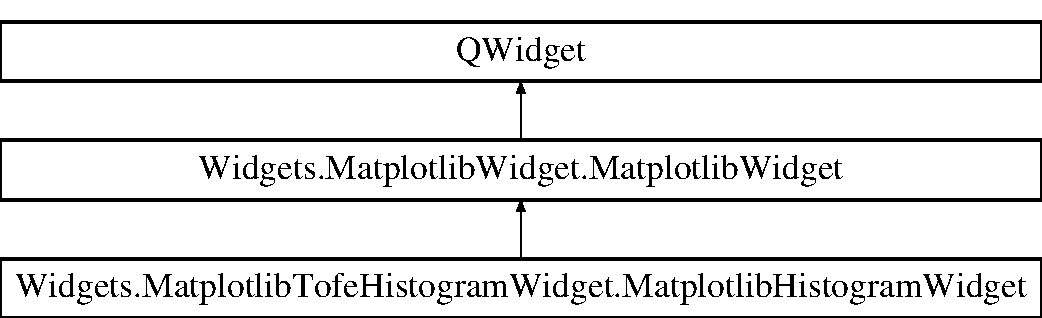
\includegraphics[height=3.000000cm]{classWidgets_1_1MatplotlibTofeHistogramWidget_1_1MatplotlibHistogramWidget}
\end{center}
\end{figure}
\subsection*{Public Member Functions}
\begin{DoxyCompactItemize}
\item 
def \hyperlink{classWidgets_1_1MatplotlibTofeHistogramWidget_1_1MatplotlibHistogramWidget_aad6c4d8bd08361b82802043538c490cb}{\-\_\-\-\_\-init\-\_\-\-\_\-}
\item 
def \hyperlink{classWidgets_1_1MatplotlibTofeHistogramWidget_1_1MatplotlibHistogramWidget_ab339aa6fbf1a155bfa55e82408479827}{on\-\_\-draw}
\item 
def \hyperlink{classWidgets_1_1MatplotlibTofeHistogramWidget_1_1MatplotlibHistogramWidget_a6b99036e842a3a10d973a24beed195e4}{on\-\_\-click}
\item 
def \hyperlink{classWidgets_1_1MatplotlibTofeHistogramWidget_1_1MatplotlibHistogramWidget_a4511fc6ceba6077d9b77c7ebc5844589}{graph\-\_\-settings\-\_\-dialog}
\item 
def \hyperlink{classWidgets_1_1MatplotlibTofeHistogramWidget_1_1MatplotlibHistogramWidget_a867b89b1e7cffc519767f42aed7aa65d}{selection\-\_\-settings\-\_\-dialog}
\item 
def \hyperlink{classWidgets_1_1MatplotlibTofeHistogramWidget_1_1MatplotlibHistogramWidget_a0e05307e27790c3630d460c8f2324e53}{load\-\_\-selections}
\item 
def \hyperlink{classWidgets_1_1MatplotlibTofeHistogramWidget_1_1MatplotlibHistogramWidget_aba4b6470b436cfdebfafd4b22b77c2c1}{save\-\_\-cuts}
\item 
def \hyperlink{classWidgets_1_1MatplotlibTofeHistogramWidget_1_1MatplotlibHistogramWidget_ae50900b6a88cfc1f79e324b926524f69}{enable\-\_\-element\-\_\-selection}
\item 
def \hyperlink{classWidgets_1_1MatplotlibTofeHistogramWidget_1_1MatplotlibHistogramWidget_a77c4e39548829cecc7b24868da5c2ab7}{enable\-\_\-selection\-\_\-select}
\item 
def \hyperlink{classWidgets_1_1MatplotlibTofeHistogramWidget_1_1MatplotlibHistogramWidget_a29d44d21a1d4159302427c6194f2bcb1}{remove\-\_\-selected}
\item 
def \hyperlink{classWidgets_1_1MatplotlibTofeHistogramWidget_1_1MatplotlibHistogramWidget_a6582d98b8bfa9c935fc55d44956ae3ec}{remove\-\_\-all\-\_\-selections}
\item 
def \hyperlink{classWidgets_1_1MatplotlibTofeHistogramWidget_1_1MatplotlibHistogramWidget_a565fdecf97e86b1c7d815fa64a7fa436}{undo\-\_\-point}
\item 
def \hyperlink{classWidgets_1_1MatplotlibTofeHistogramWidget_1_1MatplotlibHistogramWidget_a452fba4272e9c97ec1ddcab3096a90a3}{show\-\_\-yourself}
\item 
def \hyperlink{classWidgets_1_1MatplotlibTofeHistogramWidget_1_1MatplotlibHistogramWidget_a82043cfec6ce431cac9a2b8a937318ae}{sc\-\_\-comp\-\_\-inc}
\item 
def \hyperlink{classWidgets_1_1MatplotlibTofeHistogramWidget_1_1MatplotlibHistogramWidget_a56ba65f0afd7c4d61ab4264fcb2f1987}{sc\-\_\-comp\-\_\-dec}
\end{DoxyCompactItemize}
\subsection*{Public Attributes}
\begin{DoxyCompactItemize}
\item 
\hypertarget{classWidgets_1_1MatplotlibTofeHistogramWidget_1_1MatplotlibHistogramWidget_a929d308a22016759ac7dcefb1f84d4cd}{{\bfseries measurement}}\label{classWidgets_1_1MatplotlibTofeHistogramWidget_1_1MatplotlibHistogramWidget_a929d308a22016759ac7dcefb1f84d4cd}

\item 
\hypertarget{classWidgets_1_1MatplotlibTofeHistogramWidget_1_1MatplotlibHistogramWidget_a093162b04fa022d1785e99148dfc0265}{{\bfseries invert\-\_\-\-Y}}\label{classWidgets_1_1MatplotlibTofeHistogramWidget_1_1MatplotlibHistogramWidget_a093162b04fa022d1785e99148dfc0265}

\item 
\hypertarget{classWidgets_1_1MatplotlibTofeHistogramWidget_1_1MatplotlibHistogramWidget_a290b4cd93820735315db16f5d470f83c}{{\bfseries invert\-\_\-\-X}}\label{classWidgets_1_1MatplotlibTofeHistogramWidget_1_1MatplotlibHistogramWidget_a290b4cd93820735315db16f5d470f83c}

\item 
\hypertarget{classWidgets_1_1MatplotlibTofeHistogramWidget_1_1MatplotlibHistogramWidget_a17f231d1dbf645e1cc2c3de172e8514b}{{\bfseries transpose\-\_\-axes}}\label{classWidgets_1_1MatplotlibTofeHistogramWidget_1_1MatplotlibHistogramWidget_a17f231d1dbf645e1cc2c3de172e8514b}

\item 
\hypertarget{classWidgets_1_1MatplotlibTofeHistogramWidget_1_1MatplotlibHistogramWidget_a726ce5233576d4c9d3247935fc8861c7}{{\bfseries compression\-\_\-x}}\label{classWidgets_1_1MatplotlibTofeHistogramWidget_1_1MatplotlibHistogramWidget_a726ce5233576d4c9d3247935fc8861c7}

\item 
\hypertarget{classWidgets_1_1MatplotlibTofeHistogramWidget_1_1MatplotlibHistogramWidget_a4b6b728870924e8a846d406d9211ac96}{{\bfseries compression\-\_\-y}}\label{classWidgets_1_1MatplotlibTofeHistogramWidget_1_1MatplotlibHistogramWidget_a4b6b728870924e8a846d406d9211ac96}

\item 
\hypertarget{classWidgets_1_1MatplotlibTofeHistogramWidget_1_1MatplotlibHistogramWidget_a3cd97bfe14a9e7b83ddca4cbec2a49ee}{{\bfseries axes\-\_\-range\-\_\-mode}}\label{classWidgets_1_1MatplotlibTofeHistogramWidget_1_1MatplotlibHistogramWidget_a3cd97bfe14a9e7b83ddca4cbec2a49ee}

\item 
\hypertarget{classWidgets_1_1MatplotlibTofeHistogramWidget_1_1MatplotlibHistogramWidget_a5f88205c41a29ee60e5281b8c9f787b8}{{\bfseries axes\-\_\-range}}\label{classWidgets_1_1MatplotlibTofeHistogramWidget_1_1MatplotlibHistogramWidget_a5f88205c41a29ee60e5281b8c9f787b8}

\item 
\hypertarget{classWidgets_1_1MatplotlibTofeHistogramWidget_1_1MatplotlibHistogramWidget_af66d7c70eec268e9658e2bad9a781bec}{{\bfseries name\-\_\-y\-\_\-axis}}\label{classWidgets_1_1MatplotlibTofeHistogramWidget_1_1MatplotlibHistogramWidget_af66d7c70eec268e9658e2bad9a781bec}

\item 
\hypertarget{classWidgets_1_1MatplotlibTofeHistogramWidget_1_1MatplotlibHistogramWidget_aa34c41797f372028f73ee304e896df3d}{{\bfseries name\-\_\-x\-\_\-axis}}\label{classWidgets_1_1MatplotlibTofeHistogramWidget_1_1MatplotlibHistogramWidget_aa34c41797f372028f73ee304e896df3d}

\item 
\hypertarget{classWidgets_1_1MatplotlibTofeHistogramWidget_1_1MatplotlibHistogramWidget_acd0fc4347c5b2c3f066d1bcd55c85163}{{\bfseries element\-Selection\-Button}}\label{classWidgets_1_1MatplotlibTofeHistogramWidget_1_1MatplotlibHistogramWidget_acd0fc4347c5b2c3f066d1bcd55c85163}

\item 
\hypertarget{classWidgets_1_1MatplotlibTofeHistogramWidget_1_1MatplotlibHistogramWidget_a97005bddd1546f49bb094ed8c4734e19}{{\bfseries element\-Select\-Undo\-Button}}\label{classWidgets_1_1MatplotlibTofeHistogramWidget_1_1MatplotlibHistogramWidget_a97005bddd1546f49bb094ed8c4734e19}

\item 
\hypertarget{classWidgets_1_1MatplotlibTofeHistogramWidget_1_1MatplotlibHistogramWidget_ab6c0c835e5826ba4e31990d3aa23ef25}{{\bfseries element\-Selection\-Select\-Button}}\label{classWidgets_1_1MatplotlibTofeHistogramWidget_1_1MatplotlibHistogramWidget_ab6c0c835e5826ba4e31990d3aa23ef25}

\item 
\hypertarget{classWidgets_1_1MatplotlibTofeHistogramWidget_1_1MatplotlibHistogramWidget_a644d66c87fc0cd21ef9efdbe1a1f9d1a}{{\bfseries element\-Select\-Delete\-Button}}\label{classWidgets_1_1MatplotlibTofeHistogramWidget_1_1MatplotlibHistogramWidget_a644d66c87fc0cd21ef9efdbe1a1f9d1a}

\item 
\hypertarget{classWidgets_1_1MatplotlibTofeHistogramWidget_1_1MatplotlibHistogramWidget_a92290055e57d34a8d8f369e3b3c0683e}{{\bfseries element\-Selection\-Delete\-Button}}\label{classWidgets_1_1MatplotlibTofeHistogramWidget_1_1MatplotlibHistogramWidget_a92290055e57d34a8d8f369e3b3c0683e}

\end{DoxyCompactItemize}
\subsection*{Static Public Attributes}
\begin{DoxyCompactItemize}
\item 
\hypertarget{classWidgets_1_1MatplotlibTofeHistogramWidget_1_1MatplotlibHistogramWidget_a9d194c871a1fe890cbec217c18a30e99}{tuple {\bfseries selections\-Changed} = Qt\-Core.\-pyqt\-Signal(\char`\"{}Py\-Qt\-\_\-\-Py\-Object\char`\"{})}\label{classWidgets_1_1MatplotlibTofeHistogramWidget_1_1MatplotlibHistogramWidget_a9d194c871a1fe890cbec217c18a30e99}

\item 
\hypertarget{classWidgets_1_1MatplotlibTofeHistogramWidget_1_1MatplotlibHistogramWidget_a8b722e93581a986398d5d576ac8095fb}{tuple {\bfseries save\-Cuts} = Qt\-Core.\-pyqt\-Signal(\char`\"{}Py\-Qt\-\_\-\-Py\-Object\char`\"{})}\label{classWidgets_1_1MatplotlibTofeHistogramWidget_1_1MatplotlibHistogramWidget_a8b722e93581a986398d5d576ac8095fb}

\item 
dictionary {\bfseries color\-\_\-scheme}
\item 
dictionary {\bfseries tool\-\_\-modes}
\end{DoxyCompactItemize}


\subsection{Detailed Description}
\begin{DoxyVerb}Matplotlib histogram widget, used to graph "bananas" (ToF-E).
\end{DoxyVerb}
 

\subsection{Constructor \& Destructor Documentation}
\hypertarget{classWidgets_1_1MatplotlibTofeHistogramWidget_1_1MatplotlibHistogramWidget_aad6c4d8bd08361b82802043538c490cb}{\index{Widgets\-::\-Matplotlib\-Tofe\-Histogram\-Widget\-::\-Matplotlib\-Histogram\-Widget@{Widgets\-::\-Matplotlib\-Tofe\-Histogram\-Widget\-::\-Matplotlib\-Histogram\-Widget}!\-\_\-\-\_\-init\-\_\-\-\_\-@{\-\_\-\-\_\-init\-\_\-\-\_\-}}
\index{\-\_\-\-\_\-init\-\_\-\-\_\-@{\-\_\-\-\_\-init\-\_\-\-\_\-}!Widgets::MatplotlibTofeHistogramWidget::MatplotlibHistogramWidget@{Widgets\-::\-Matplotlib\-Tofe\-Histogram\-Widget\-::\-Matplotlib\-Histogram\-Widget}}
\subsubsection[{\-\_\-\-\_\-init\-\_\-\-\_\-}]{\setlength{\rightskip}{0pt plus 5cm}def Widgets.\-Matplotlib\-Tofe\-Histogram\-Widget.\-Matplotlib\-Histogram\-Widget.\-\_\-\-\_\-init\-\_\-\-\_\- (
\begin{DoxyParamCaption}
\item[{}]{self, }
\item[{}]{parent, }
\item[{}]{measurement\-\_\-data, }
\item[{}]{masses, }
\item[{}]{icon\-\_\-manager}
\end{DoxyParamCaption}
)}}\label{classWidgets_1_1MatplotlibTofeHistogramWidget_1_1MatplotlibHistogramWidget_aad6c4d8bd08361b82802043538c490cb}
\begin{DoxyVerb}Inits histogram widget

Args:
    parent: A TofeHistogramWidget class object.
    measurement_data: A list of data points.
    icon_manager: IconManager class object.
    masses: A masses class object.
    icon_manager: An iconmanager class object.
\end{DoxyVerb}
 

\subsection{Member Function Documentation}
\hypertarget{classWidgets_1_1MatplotlibTofeHistogramWidget_1_1MatplotlibHistogramWidget_ae50900b6a88cfc1f79e324b926524f69}{\index{Widgets\-::\-Matplotlib\-Tofe\-Histogram\-Widget\-::\-Matplotlib\-Histogram\-Widget@{Widgets\-::\-Matplotlib\-Tofe\-Histogram\-Widget\-::\-Matplotlib\-Histogram\-Widget}!enable\-\_\-element\-\_\-selection@{enable\-\_\-element\-\_\-selection}}
\index{enable\-\_\-element\-\_\-selection@{enable\-\_\-element\-\_\-selection}!Widgets::MatplotlibTofeHistogramWidget::MatplotlibHistogramWidget@{Widgets\-::\-Matplotlib\-Tofe\-Histogram\-Widget\-::\-Matplotlib\-Histogram\-Widget}}
\subsubsection[{enable\-\_\-element\-\_\-selection}]{\setlength{\rightskip}{0pt plus 5cm}def Widgets.\-Matplotlib\-Tofe\-Histogram\-Widget.\-Matplotlib\-Histogram\-Widget.\-enable\-\_\-element\-\_\-selection (
\begin{DoxyParamCaption}
\item[{}]{self}
\end{DoxyParamCaption}
)}}\label{classWidgets_1_1MatplotlibTofeHistogramWidget_1_1MatplotlibHistogramWidget_ae50900b6a88cfc1f79e324b926524f69}
\begin{DoxyVerb}Enable element selection.
\end{DoxyVerb}
 \hypertarget{classWidgets_1_1MatplotlibTofeHistogramWidget_1_1MatplotlibHistogramWidget_a77c4e39548829cecc7b24868da5c2ab7}{\index{Widgets\-::\-Matplotlib\-Tofe\-Histogram\-Widget\-::\-Matplotlib\-Histogram\-Widget@{Widgets\-::\-Matplotlib\-Tofe\-Histogram\-Widget\-::\-Matplotlib\-Histogram\-Widget}!enable\-\_\-selection\-\_\-select@{enable\-\_\-selection\-\_\-select}}
\index{enable\-\_\-selection\-\_\-select@{enable\-\_\-selection\-\_\-select}!Widgets::MatplotlibTofeHistogramWidget::MatplotlibHistogramWidget@{Widgets\-::\-Matplotlib\-Tofe\-Histogram\-Widget\-::\-Matplotlib\-Histogram\-Widget}}
\subsubsection[{enable\-\_\-selection\-\_\-select}]{\setlength{\rightskip}{0pt plus 5cm}def Widgets.\-Matplotlib\-Tofe\-Histogram\-Widget.\-Matplotlib\-Histogram\-Widget.\-enable\-\_\-selection\-\_\-select (
\begin{DoxyParamCaption}
\item[{}]{self}
\end{DoxyParamCaption}
)}}\label{classWidgets_1_1MatplotlibTofeHistogramWidget_1_1MatplotlibHistogramWidget_a77c4e39548829cecc7b24868da5c2ab7}
\begin{DoxyVerb}Enable selection selecting tool.
\end{DoxyVerb}
 \hypertarget{classWidgets_1_1MatplotlibTofeHistogramWidget_1_1MatplotlibHistogramWidget_a4511fc6ceba6077d9b77c7ebc5844589}{\index{Widgets\-::\-Matplotlib\-Tofe\-Histogram\-Widget\-::\-Matplotlib\-Histogram\-Widget@{Widgets\-::\-Matplotlib\-Tofe\-Histogram\-Widget\-::\-Matplotlib\-Histogram\-Widget}!graph\-\_\-settings\-\_\-dialog@{graph\-\_\-settings\-\_\-dialog}}
\index{graph\-\_\-settings\-\_\-dialog@{graph\-\_\-settings\-\_\-dialog}!Widgets::MatplotlibTofeHistogramWidget::MatplotlibHistogramWidget@{Widgets\-::\-Matplotlib\-Tofe\-Histogram\-Widget\-::\-Matplotlib\-Histogram\-Widget}}
\subsubsection[{graph\-\_\-settings\-\_\-dialog}]{\setlength{\rightskip}{0pt plus 5cm}def Widgets.\-Matplotlib\-Tofe\-Histogram\-Widget.\-Matplotlib\-Histogram\-Widget.\-graph\-\_\-settings\-\_\-dialog (
\begin{DoxyParamCaption}
\item[{}]{self}
\end{DoxyParamCaption}
)}}\label{classWidgets_1_1MatplotlibTofeHistogramWidget_1_1MatplotlibHistogramWidget_a4511fc6ceba6077d9b77c7ebc5844589}
\begin{DoxyVerb}Show graph settings dialog.
\end{DoxyVerb}
 \hypertarget{classWidgets_1_1MatplotlibTofeHistogramWidget_1_1MatplotlibHistogramWidget_a0e05307e27790c3630d460c8f2324e53}{\index{Widgets\-::\-Matplotlib\-Tofe\-Histogram\-Widget\-::\-Matplotlib\-Histogram\-Widget@{Widgets\-::\-Matplotlib\-Tofe\-Histogram\-Widget\-::\-Matplotlib\-Histogram\-Widget}!load\-\_\-selections@{load\-\_\-selections}}
\index{load\-\_\-selections@{load\-\_\-selections}!Widgets::MatplotlibTofeHistogramWidget::MatplotlibHistogramWidget@{Widgets\-::\-Matplotlib\-Tofe\-Histogram\-Widget\-::\-Matplotlib\-Histogram\-Widget}}
\subsubsection[{load\-\_\-selections}]{\setlength{\rightskip}{0pt plus 5cm}def Widgets.\-Matplotlib\-Tofe\-Histogram\-Widget.\-Matplotlib\-Histogram\-Widget.\-load\-\_\-selections (
\begin{DoxyParamCaption}
\item[{}]{self}
\end{DoxyParamCaption}
)}}\label{classWidgets_1_1MatplotlibTofeHistogramWidget_1_1MatplotlibHistogramWidget_a0e05307e27790c3630d460c8f2324e53}
\begin{DoxyVerb}Show dialog to load selections.
\end{DoxyVerb}
 \hypertarget{classWidgets_1_1MatplotlibTofeHistogramWidget_1_1MatplotlibHistogramWidget_a6b99036e842a3a10d973a24beed195e4}{\index{Widgets\-::\-Matplotlib\-Tofe\-Histogram\-Widget\-::\-Matplotlib\-Histogram\-Widget@{Widgets\-::\-Matplotlib\-Tofe\-Histogram\-Widget\-::\-Matplotlib\-Histogram\-Widget}!on\-\_\-click@{on\-\_\-click}}
\index{on\-\_\-click@{on\-\_\-click}!Widgets::MatplotlibTofeHistogramWidget::MatplotlibHistogramWidget@{Widgets\-::\-Matplotlib\-Tofe\-Histogram\-Widget\-::\-Matplotlib\-Histogram\-Widget}}
\subsubsection[{on\-\_\-click}]{\setlength{\rightskip}{0pt plus 5cm}def Widgets.\-Matplotlib\-Tofe\-Histogram\-Widget.\-Matplotlib\-Histogram\-Widget.\-on\-\_\-click (
\begin{DoxyParamCaption}
\item[{}]{self, }
\item[{}]{event}
\end{DoxyParamCaption}
)}}\label{classWidgets_1_1MatplotlibTofeHistogramWidget_1_1MatplotlibHistogramWidget_a6b99036e842a3a10d973a24beed195e4}
\begin{DoxyVerb}On click event above graph.

Args:
    event: A MPL MouseEvent
\end{DoxyVerb}
 \hypertarget{classWidgets_1_1MatplotlibTofeHistogramWidget_1_1MatplotlibHistogramWidget_ab339aa6fbf1a155bfa55e82408479827}{\index{Widgets\-::\-Matplotlib\-Tofe\-Histogram\-Widget\-::\-Matplotlib\-Histogram\-Widget@{Widgets\-::\-Matplotlib\-Tofe\-Histogram\-Widget\-::\-Matplotlib\-Histogram\-Widget}!on\-\_\-draw@{on\-\_\-draw}}
\index{on\-\_\-draw@{on\-\_\-draw}!Widgets::MatplotlibTofeHistogramWidget::MatplotlibHistogramWidget@{Widgets\-::\-Matplotlib\-Tofe\-Histogram\-Widget\-::\-Matplotlib\-Histogram\-Widget}}
\subsubsection[{on\-\_\-draw}]{\setlength{\rightskip}{0pt plus 5cm}def Widgets.\-Matplotlib\-Tofe\-Histogram\-Widget.\-Matplotlib\-Histogram\-Widget.\-on\-\_\-draw (
\begin{DoxyParamCaption}
\item[{}]{self}
\end{DoxyParamCaption}
)}}\label{classWidgets_1_1MatplotlibTofeHistogramWidget_1_1MatplotlibHistogramWidget_ab339aa6fbf1a155bfa55e82408479827}
\begin{DoxyVerb}Draw method for matplotlib.
\end{DoxyVerb}
 \hypertarget{classWidgets_1_1MatplotlibTofeHistogramWidget_1_1MatplotlibHistogramWidget_a6582d98b8bfa9c935fc55d44956ae3ec}{\index{Widgets\-::\-Matplotlib\-Tofe\-Histogram\-Widget\-::\-Matplotlib\-Histogram\-Widget@{Widgets\-::\-Matplotlib\-Tofe\-Histogram\-Widget\-::\-Matplotlib\-Histogram\-Widget}!remove\-\_\-all\-\_\-selections@{remove\-\_\-all\-\_\-selections}}
\index{remove\-\_\-all\-\_\-selections@{remove\-\_\-all\-\_\-selections}!Widgets::MatplotlibTofeHistogramWidget::MatplotlibHistogramWidget@{Widgets\-::\-Matplotlib\-Tofe\-Histogram\-Widget\-::\-Matplotlib\-Histogram\-Widget}}
\subsubsection[{remove\-\_\-all\-\_\-selections}]{\setlength{\rightskip}{0pt plus 5cm}def Widgets.\-Matplotlib\-Tofe\-Histogram\-Widget.\-Matplotlib\-Histogram\-Widget.\-remove\-\_\-all\-\_\-selections (
\begin{DoxyParamCaption}
\item[{}]{self}
\end{DoxyParamCaption}
)}}\label{classWidgets_1_1MatplotlibTofeHistogramWidget_1_1MatplotlibHistogramWidget_a6582d98b8bfa9c935fc55d44956ae3ec}
\begin{DoxyVerb}Remove all selections.
\end{DoxyVerb}
 \hypertarget{classWidgets_1_1MatplotlibTofeHistogramWidget_1_1MatplotlibHistogramWidget_a29d44d21a1d4159302427c6194f2bcb1}{\index{Widgets\-::\-Matplotlib\-Tofe\-Histogram\-Widget\-::\-Matplotlib\-Histogram\-Widget@{Widgets\-::\-Matplotlib\-Tofe\-Histogram\-Widget\-::\-Matplotlib\-Histogram\-Widget}!remove\-\_\-selected@{remove\-\_\-selected}}
\index{remove\-\_\-selected@{remove\-\_\-selected}!Widgets::MatplotlibTofeHistogramWidget::MatplotlibHistogramWidget@{Widgets\-::\-Matplotlib\-Tofe\-Histogram\-Widget\-::\-Matplotlib\-Histogram\-Widget}}
\subsubsection[{remove\-\_\-selected}]{\setlength{\rightskip}{0pt plus 5cm}def Widgets.\-Matplotlib\-Tofe\-Histogram\-Widget.\-Matplotlib\-Histogram\-Widget.\-remove\-\_\-selected (
\begin{DoxyParamCaption}
\item[{}]{self}
\end{DoxyParamCaption}
)}}\label{classWidgets_1_1MatplotlibTofeHistogramWidget_1_1MatplotlibHistogramWidget_a29d44d21a1d4159302427c6194f2bcb1}
\begin{DoxyVerb}Remove selected selection.
\end{DoxyVerb}
 \hypertarget{classWidgets_1_1MatplotlibTofeHistogramWidget_1_1MatplotlibHistogramWidget_aba4b6470b436cfdebfafd4b22b77c2c1}{\index{Widgets\-::\-Matplotlib\-Tofe\-Histogram\-Widget\-::\-Matplotlib\-Histogram\-Widget@{Widgets\-::\-Matplotlib\-Tofe\-Histogram\-Widget\-::\-Matplotlib\-Histogram\-Widget}!save\-\_\-cuts@{save\-\_\-cuts}}
\index{save\-\_\-cuts@{save\-\_\-cuts}!Widgets::MatplotlibTofeHistogramWidget::MatplotlibHistogramWidget@{Widgets\-::\-Matplotlib\-Tofe\-Histogram\-Widget\-::\-Matplotlib\-Histogram\-Widget}}
\subsubsection[{save\-\_\-cuts}]{\setlength{\rightskip}{0pt plus 5cm}def Widgets.\-Matplotlib\-Tofe\-Histogram\-Widget.\-Matplotlib\-Histogram\-Widget.\-save\-\_\-cuts (
\begin{DoxyParamCaption}
\item[{}]{self}
\end{DoxyParamCaption}
)}}\label{classWidgets_1_1MatplotlibTofeHistogramWidget_1_1MatplotlibHistogramWidget_aba4b6470b436cfdebfafd4b22b77c2c1}
\begin{DoxyVerb}Save measurement cuts.
\end{DoxyVerb}
 \hypertarget{classWidgets_1_1MatplotlibTofeHistogramWidget_1_1MatplotlibHistogramWidget_a56ba65f0afd7c4d61ab4264fcb2f1987}{\index{Widgets\-::\-Matplotlib\-Tofe\-Histogram\-Widget\-::\-Matplotlib\-Histogram\-Widget@{Widgets\-::\-Matplotlib\-Tofe\-Histogram\-Widget\-::\-Matplotlib\-Histogram\-Widget}!sc\-\_\-comp\-\_\-dec@{sc\-\_\-comp\-\_\-dec}}
\index{sc\-\_\-comp\-\_\-dec@{sc\-\_\-comp\-\_\-dec}!Widgets::MatplotlibTofeHistogramWidget::MatplotlibHistogramWidget@{Widgets\-::\-Matplotlib\-Tofe\-Histogram\-Widget\-::\-Matplotlib\-Histogram\-Widget}}
\subsubsection[{sc\-\_\-comp\-\_\-dec}]{\setlength{\rightskip}{0pt plus 5cm}def Widgets.\-Matplotlib\-Tofe\-Histogram\-Widget.\-Matplotlib\-Histogram\-Widget.\-sc\-\_\-comp\-\_\-dec (
\begin{DoxyParamCaption}
\item[{}]{self, }
\item[{}]{mode}
\end{DoxyParamCaption}
)}}\label{classWidgets_1_1MatplotlibTofeHistogramWidget_1_1MatplotlibHistogramWidget_a56ba65f0afd7c4d61ab4264fcb2f1987}
\begin{DoxyVerb}Shortcut to decrease compression factor.

Args:
    mode: An integer representing axis or axes to change.
\end{DoxyVerb}
 \hypertarget{classWidgets_1_1MatplotlibTofeHistogramWidget_1_1MatplotlibHistogramWidget_a82043cfec6ce431cac9a2b8a937318ae}{\index{Widgets\-::\-Matplotlib\-Tofe\-Histogram\-Widget\-::\-Matplotlib\-Histogram\-Widget@{Widgets\-::\-Matplotlib\-Tofe\-Histogram\-Widget\-::\-Matplotlib\-Histogram\-Widget}!sc\-\_\-comp\-\_\-inc@{sc\-\_\-comp\-\_\-inc}}
\index{sc\-\_\-comp\-\_\-inc@{sc\-\_\-comp\-\_\-inc}!Widgets::MatplotlibTofeHistogramWidget::MatplotlibHistogramWidget@{Widgets\-::\-Matplotlib\-Tofe\-Histogram\-Widget\-::\-Matplotlib\-Histogram\-Widget}}
\subsubsection[{sc\-\_\-comp\-\_\-inc}]{\setlength{\rightskip}{0pt plus 5cm}def Widgets.\-Matplotlib\-Tofe\-Histogram\-Widget.\-Matplotlib\-Histogram\-Widget.\-sc\-\_\-comp\-\_\-inc (
\begin{DoxyParamCaption}
\item[{}]{self, }
\item[{}]{mode}
\end{DoxyParamCaption}
)}}\label{classWidgets_1_1MatplotlibTofeHistogramWidget_1_1MatplotlibHistogramWidget_a82043cfec6ce431cac9a2b8a937318ae}
\begin{DoxyVerb}Shortcut to increase compression factor.

Args:
    mode: An integer representing axis or axes to change.
\end{DoxyVerb}
 \hypertarget{classWidgets_1_1MatplotlibTofeHistogramWidget_1_1MatplotlibHistogramWidget_a867b89b1e7cffc519767f42aed7aa65d}{\index{Widgets\-::\-Matplotlib\-Tofe\-Histogram\-Widget\-::\-Matplotlib\-Histogram\-Widget@{Widgets\-::\-Matplotlib\-Tofe\-Histogram\-Widget\-::\-Matplotlib\-Histogram\-Widget}!selection\-\_\-settings\-\_\-dialog@{selection\-\_\-settings\-\_\-dialog}}
\index{selection\-\_\-settings\-\_\-dialog@{selection\-\_\-settings\-\_\-dialog}!Widgets::MatplotlibTofeHistogramWidget::MatplotlibHistogramWidget@{Widgets\-::\-Matplotlib\-Tofe\-Histogram\-Widget\-::\-Matplotlib\-Histogram\-Widget}}
\subsubsection[{selection\-\_\-settings\-\_\-dialog}]{\setlength{\rightskip}{0pt plus 5cm}def Widgets.\-Matplotlib\-Tofe\-Histogram\-Widget.\-Matplotlib\-Histogram\-Widget.\-selection\-\_\-settings\-\_\-dialog (
\begin{DoxyParamCaption}
\item[{}]{self}
\end{DoxyParamCaption}
)}}\label{classWidgets_1_1MatplotlibTofeHistogramWidget_1_1MatplotlibHistogramWidget_a867b89b1e7cffc519767f42aed7aa65d}
\begin{DoxyVerb}Show selection settings dialog.
\end{DoxyVerb}
 \hypertarget{classWidgets_1_1MatplotlibTofeHistogramWidget_1_1MatplotlibHistogramWidget_a452fba4272e9c97ec1ddcab3096a90a3}{\index{Widgets\-::\-Matplotlib\-Tofe\-Histogram\-Widget\-::\-Matplotlib\-Histogram\-Widget@{Widgets\-::\-Matplotlib\-Tofe\-Histogram\-Widget\-::\-Matplotlib\-Histogram\-Widget}!show\-\_\-yourself@{show\-\_\-yourself}}
\index{show\-\_\-yourself@{show\-\_\-yourself}!Widgets::MatplotlibTofeHistogramWidget::MatplotlibHistogramWidget@{Widgets\-::\-Matplotlib\-Tofe\-Histogram\-Widget\-::\-Matplotlib\-Histogram\-Widget}}
\subsubsection[{show\-\_\-yourself}]{\setlength{\rightskip}{0pt plus 5cm}def Widgets.\-Matplotlib\-Tofe\-Histogram\-Widget.\-Matplotlib\-Histogram\-Widget.\-show\-\_\-yourself (
\begin{DoxyParamCaption}
\item[{}]{self, }
\item[{}]{ui}
\end{DoxyParamCaption}
)}}\label{classWidgets_1_1MatplotlibTofeHistogramWidget_1_1MatplotlibHistogramWidget_a452fba4272e9c97ec1ddcab3096a90a3}
\begin{DoxyVerb}Show ToF-E histogram settings in ui.

Args:
    ui: A TofeGraphSettingsWidget's .ui file variable.
\end{DoxyVerb}
 \hypertarget{classWidgets_1_1MatplotlibTofeHistogramWidget_1_1MatplotlibHistogramWidget_a565fdecf97e86b1c7d815fa64a7fa436}{\index{Widgets\-::\-Matplotlib\-Tofe\-Histogram\-Widget\-::\-Matplotlib\-Histogram\-Widget@{Widgets\-::\-Matplotlib\-Tofe\-Histogram\-Widget\-::\-Matplotlib\-Histogram\-Widget}!undo\-\_\-point@{undo\-\_\-point}}
\index{undo\-\_\-point@{undo\-\_\-point}!Widgets::MatplotlibTofeHistogramWidget::MatplotlibHistogramWidget@{Widgets\-::\-Matplotlib\-Tofe\-Histogram\-Widget\-::\-Matplotlib\-Histogram\-Widget}}
\subsubsection[{undo\-\_\-point}]{\setlength{\rightskip}{0pt plus 5cm}def Widgets.\-Matplotlib\-Tofe\-Histogram\-Widget.\-Matplotlib\-Histogram\-Widget.\-undo\-\_\-point (
\begin{DoxyParamCaption}
\item[{}]{self}
\end{DoxyParamCaption}
)}}\label{classWidgets_1_1MatplotlibTofeHistogramWidget_1_1MatplotlibHistogramWidget_a565fdecf97e86b1c7d815fa64a7fa436}
\begin{DoxyVerb}Undo last point in open selection.
\end{DoxyVerb}
 

\subsection{Member Data Documentation}
\hypertarget{classWidgets_1_1MatplotlibTofeHistogramWidget_1_1MatplotlibHistogramWidget_ad26db4a8040143bd1678bb1f41b8c9d8}{\index{Widgets\-::\-Matplotlib\-Tofe\-Histogram\-Widget\-::\-Matplotlib\-Histogram\-Widget@{Widgets\-::\-Matplotlib\-Tofe\-Histogram\-Widget\-::\-Matplotlib\-Histogram\-Widget}!color\-\_\-scheme@{color\-\_\-scheme}}
\index{color\-\_\-scheme@{color\-\_\-scheme}!Widgets::MatplotlibTofeHistogramWidget::MatplotlibHistogramWidget@{Widgets\-::\-Matplotlib\-Tofe\-Histogram\-Widget\-::\-Matplotlib\-Histogram\-Widget}}
\subsubsection[{color\-\_\-scheme}]{\setlength{\rightskip}{0pt plus 5cm}dictionary Widgets.\-Matplotlib\-Tofe\-Histogram\-Widget.\-Matplotlib\-Histogram\-Widget.\-color\-\_\-scheme\hspace{0.3cm}{\ttfamily [static]}}}\label{classWidgets_1_1MatplotlibTofeHistogramWidget_1_1MatplotlibHistogramWidget_ad26db4a8040143bd1678bb1f41b8c9d8}
{\bfseries Initial value\-:}
\begin{DoxyCode}
1 = \{\textcolor{stringliteral}{"Default color"}:\textcolor{stringliteral}{"jet"},
2                     \textcolor{stringliteral}{"Greyscale"}:\textcolor{stringliteral}{"Greys"},
3                     \textcolor{stringliteral}{"Greyscale (inverted)"}:\textcolor{stringliteral}{"gray"}\}
\end{DoxyCode}
\hypertarget{classWidgets_1_1MatplotlibTofeHistogramWidget_1_1MatplotlibHistogramWidget_a24f1bc714cd9f115d6c9d0f304c6de3c}{\index{Widgets\-::\-Matplotlib\-Tofe\-Histogram\-Widget\-::\-Matplotlib\-Histogram\-Widget@{Widgets\-::\-Matplotlib\-Tofe\-Histogram\-Widget\-::\-Matplotlib\-Histogram\-Widget}!tool\-\_\-modes@{tool\-\_\-modes}}
\index{tool\-\_\-modes@{tool\-\_\-modes}!Widgets::MatplotlibTofeHistogramWidget::MatplotlibHistogramWidget@{Widgets\-::\-Matplotlib\-Tofe\-Histogram\-Widget\-::\-Matplotlib\-Histogram\-Widget}}
\subsubsection[{tool\-\_\-modes}]{\setlength{\rightskip}{0pt plus 5cm}dictionary Widgets.\-Matplotlib\-Tofe\-Histogram\-Widget.\-Matplotlib\-Histogram\-Widget.\-tool\-\_\-modes\hspace{0.3cm}{\ttfamily [static]}}}\label{classWidgets_1_1MatplotlibTofeHistogramWidget_1_1MatplotlibHistogramWidget_a24f1bc714cd9f115d6c9d0f304c6de3c}
{\bfseries Initial value\-:}
\begin{DoxyCode}
1 = \{ 0 : \textcolor{stringliteral}{""},
2                    1 : \textcolor{stringliteral}{"pan/zoom"},  \textcolor{comment}{# Matplotlib's drag}
3                    2 : \textcolor{stringliteral}{"zoom rect"},  \textcolor{comment}{# Matplotlib's zoom}
4                    3 : \textcolor{stringliteral}{"selection tool"},
5                    4 : \textcolor{stringliteral}{"selection select tool"}
6                   \}
\end{DoxyCode}


The documentation for this class was generated from the following file\-:\begin{DoxyCompactItemize}
\item 
Widgets/Matplotlib\-Tofe\-Histogram\-Widget.\-py\end{DoxyCompactItemize}

\hypertarget{classWidgets_1_1MatplotlibImportTimingWidget_1_1MatplotlibImportTimingWidget}{\section{Widgets.\-Matplotlib\-Import\-Timing\-Widget.\-Matplotlib\-Import\-Timing\-Widget Class Reference}
\label{classWidgets_1_1MatplotlibImportTimingWidget_1_1MatplotlibImportTimingWidget}\index{Widgets.\-Matplotlib\-Import\-Timing\-Widget.\-Matplotlib\-Import\-Timing\-Widget@{Widgets.\-Matplotlib\-Import\-Timing\-Widget.\-Matplotlib\-Import\-Timing\-Widget}}
}
Inheritance diagram for Widgets.\-Matplotlib\-Import\-Timing\-Widget.\-Matplotlib\-Import\-Timing\-Widget\-:\begin{figure}[H]
\begin{center}
\leavevmode
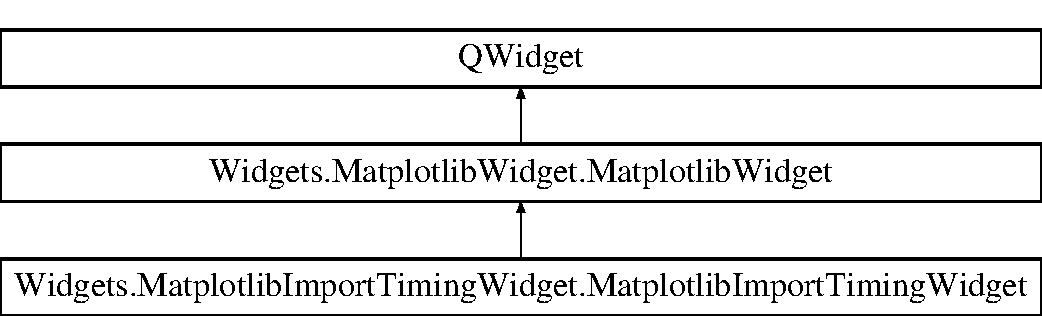
\includegraphics[height=3.000000cm]{classWidgets_1_1MatplotlibImportTimingWidget_1_1MatplotlibImportTimingWidget}
\end{center}
\end{figure}
\subsection*{Public Member Functions}
\begin{DoxyCompactItemize}
\item 
def \hyperlink{classWidgets_1_1MatplotlibImportTimingWidget_1_1MatplotlibImportTimingWidget_ae14615610f18f54d5fc711b262a63bd6}{\-\_\-\-\_\-init\-\_\-\-\_\-}
\item 
def \hyperlink{classWidgets_1_1MatplotlibImportTimingWidget_1_1MatplotlibImportTimingWidget_a040c772973ab8852b0ac2d13a594b7de}{on\-\_\-draw}
\item 
def \hyperlink{classWidgets_1_1MatplotlibImportTimingWidget_1_1MatplotlibImportTimingWidget_a6ae365302597a376c26abd756f64feda}{on\-\_\-click}
\end{DoxyCompactItemize}
\subsection*{Public Attributes}
\begin{DoxyCompactItemize}
\item 
\hypertarget{classWidgets_1_1MatplotlibImportTimingWidget_1_1MatplotlibImportTimingWidget_a60874165b2db9c8ca5aa9086ee4e7821}{{\bfseries icon\-\_\-manager}}\label{classWidgets_1_1MatplotlibImportTimingWidget_1_1MatplotlibImportTimingWidget_a60874165b2db9c8ca5aa9086ee4e7821}

\item 
\hypertarget{classWidgets_1_1MatplotlibImportTimingWidget_1_1MatplotlibImportTimingWidget_a26e1973fc4b3066638df749b4b89bf8f}{{\bfseries data}}\label{classWidgets_1_1MatplotlibImportTimingWidget_1_1MatplotlibImportTimingWidget_a26e1973fc4b3066638df749b4b89bf8f}

\item 
\hypertarget{classWidgets_1_1MatplotlibImportTimingWidget_1_1MatplotlibImportTimingWidget_a93e26e6511f1dc77a96eb2144bcf9222}{{\bfseries lim\-Button}}\label{classWidgets_1_1MatplotlibImportTimingWidget_1_1MatplotlibImportTimingWidget_a93e26e6511f1dc77a96eb2144bcf9222}

\end{DoxyCompactItemize}


\subsection{Constructor \& Destructor Documentation}
\hypertarget{classWidgets_1_1MatplotlibImportTimingWidget_1_1MatplotlibImportTimingWidget_ae14615610f18f54d5fc711b262a63bd6}{\index{Widgets\-::\-Matplotlib\-Import\-Timing\-Widget\-::\-Matplotlib\-Import\-Timing\-Widget@{Widgets\-::\-Matplotlib\-Import\-Timing\-Widget\-::\-Matplotlib\-Import\-Timing\-Widget}!\-\_\-\-\_\-init\-\_\-\-\_\-@{\-\_\-\-\_\-init\-\_\-\-\_\-}}
\index{\-\_\-\-\_\-init\-\_\-\-\_\-@{\-\_\-\-\_\-init\-\_\-\-\_\-}!Widgets::MatplotlibImportTimingWidget::MatplotlibImportTimingWidget@{Widgets\-::\-Matplotlib\-Import\-Timing\-Widget\-::\-Matplotlib\-Import\-Timing\-Widget}}
\subsubsection[{\-\_\-\-\_\-init\-\_\-\-\_\-}]{\setlength{\rightskip}{0pt plus 5cm}def Widgets.\-Matplotlib\-Import\-Timing\-Widget.\-Matplotlib\-Import\-Timing\-Widget.\-\_\-\-\_\-init\-\_\-\-\_\- (
\begin{DoxyParamCaption}
\item[{}]{self, }
\item[{}]{parent, }
\item[{}]{output\-\_\-file, }
\item[{}]{icon\-\_\-manager, }
\item[{}]{timing}
\end{DoxyParamCaption}
)}}\label{classWidgets_1_1MatplotlibImportTimingWidget_1_1MatplotlibImportTimingWidget_ae14615610f18f54d5fc711b262a63bd6}
\begin{DoxyVerb}Inits import timings widget

Args:
    parent: An ImportTimingGraphDialog class object.
    output_file: A string representing file to be graphed.
    icon_manager: An IconManager class object.
    timing: A tuple representing low & high timing limits.
\end{DoxyVerb}
 

\subsection{Member Function Documentation}
\hypertarget{classWidgets_1_1MatplotlibImportTimingWidget_1_1MatplotlibImportTimingWidget_a6ae365302597a376c26abd756f64feda}{\index{Widgets\-::\-Matplotlib\-Import\-Timing\-Widget\-::\-Matplotlib\-Import\-Timing\-Widget@{Widgets\-::\-Matplotlib\-Import\-Timing\-Widget\-::\-Matplotlib\-Import\-Timing\-Widget}!on\-\_\-click@{on\-\_\-click}}
\index{on\-\_\-click@{on\-\_\-click}!Widgets::MatplotlibImportTimingWidget::MatplotlibImportTimingWidget@{Widgets\-::\-Matplotlib\-Import\-Timing\-Widget\-::\-Matplotlib\-Import\-Timing\-Widget}}
\subsubsection[{on\-\_\-click}]{\setlength{\rightskip}{0pt plus 5cm}def Widgets.\-Matplotlib\-Import\-Timing\-Widget.\-Matplotlib\-Import\-Timing\-Widget.\-on\-\_\-click (
\begin{DoxyParamCaption}
\item[{}]{self, }
\item[{}]{event}
\end{DoxyParamCaption}
)}}\label{classWidgets_1_1MatplotlibImportTimingWidget_1_1MatplotlibImportTimingWidget_a6ae365302597a376c26abd756f64feda}
\begin{DoxyVerb}Handles clicks on the graph.

Args:
    event: A click event on the graph
\end{DoxyVerb}
 \hypertarget{classWidgets_1_1MatplotlibImportTimingWidget_1_1MatplotlibImportTimingWidget_a040c772973ab8852b0ac2d13a594b7de}{\index{Widgets\-::\-Matplotlib\-Import\-Timing\-Widget\-::\-Matplotlib\-Import\-Timing\-Widget@{Widgets\-::\-Matplotlib\-Import\-Timing\-Widget\-::\-Matplotlib\-Import\-Timing\-Widget}!on\-\_\-draw@{on\-\_\-draw}}
\index{on\-\_\-draw@{on\-\_\-draw}!Widgets::MatplotlibImportTimingWidget::MatplotlibImportTimingWidget@{Widgets\-::\-Matplotlib\-Import\-Timing\-Widget\-::\-Matplotlib\-Import\-Timing\-Widget}}
\subsubsection[{on\-\_\-draw}]{\setlength{\rightskip}{0pt plus 5cm}def Widgets.\-Matplotlib\-Import\-Timing\-Widget.\-Matplotlib\-Import\-Timing\-Widget.\-on\-\_\-draw (
\begin{DoxyParamCaption}
\item[{}]{self}
\end{DoxyParamCaption}
)}}\label{classWidgets_1_1MatplotlibImportTimingWidget_1_1MatplotlibImportTimingWidget_a040c772973ab8852b0ac2d13a594b7de}
\begin{DoxyVerb}Draws the timings graph
\end{DoxyVerb}
 

The documentation for this class was generated from the following file\-:\begin{DoxyCompactItemize}
\item 
Widgets/Matplotlib\-Import\-Timing\-Widget.\-py\end{DoxyCompactItemize}

\hypertarget{classWidgets_1_1MatplotlibWidget_1_1MatplotlibWidget}{\section{Widgets.\-Matplotlib\-Widget.\-Matplotlib\-Widget Class Reference}
\label{classWidgets_1_1MatplotlibWidget_1_1MatplotlibWidget}\index{Widgets.\-Matplotlib\-Widget.\-Matplotlib\-Widget@{Widgets.\-Matplotlib\-Widget.\-Matplotlib\-Widget}}
}
Inheritance diagram for Widgets.\-Matplotlib\-Widget.\-Matplotlib\-Widget\-:\begin{figure}[H]
\begin{center}
\leavevmode
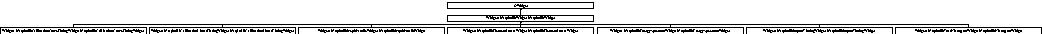
\includegraphics[height=0.463320cm]{classWidgets_1_1MatplotlibWidget_1_1MatplotlibWidget}
\end{center}
\end{figure}
\subsection*{Public Member Functions}
\begin{DoxyCompactItemize}
\item 
def \hyperlink{classWidgets_1_1MatplotlibWidget_1_1MatplotlibWidget_a61cf93497bbdd82f5f6b62a074ab47b2}{\-\_\-\-\_\-init\-\_\-\-\_\-}
\item 
def \hyperlink{classWidgets_1_1MatplotlibWidget_1_1MatplotlibWidget_a4e4b2d118d14e76c0ff72b45f8cce460}{fork\-\_\-toolbar\-\_\-buttons}
\item 
def \hyperlink{classWidgets_1_1MatplotlibWidget_1_1MatplotlibWidget_a4ed271205f620e901ac55429b599bad4}{remove\-\_\-axes\-\_\-ticks}
\item 
def \hyperlink{classWidgets_1_1MatplotlibWidget_1_1MatplotlibWidget_aae8259a60c7e1e2989985e39dadf23da}{delete}
\end{DoxyCompactItemize}
\subsection*{Public Attributes}
\begin{DoxyCompactItemize}
\item 
\hypertarget{classWidgets_1_1MatplotlibWidget_1_1MatplotlibWidget_aa6acd64282989e5bc6404bd5a7572607}{{\bfseries main\-\_\-frame}}\label{classWidgets_1_1MatplotlibWidget_1_1MatplotlibWidget_aa6acd64282989e5bc6404bd5a7572607}

\item 
\hypertarget{classWidgets_1_1MatplotlibWidget_1_1MatplotlibWidget_a942589dd31667ef15d1ba5467839360a}{{\bfseries dpi}}\label{classWidgets_1_1MatplotlibWidget_1_1MatplotlibWidget_a942589dd31667ef15d1ba5467839360a}

\item 
\hypertarget{classWidgets_1_1MatplotlibWidget_1_1MatplotlibWidget_ad69c051a114fe8e0ba4eb47084202f05}{{\bfseries show\-\_\-axis\-\_\-ticks}}\label{classWidgets_1_1MatplotlibWidget_1_1MatplotlibWidget_ad69c051a114fe8e0ba4eb47084202f05}

\item 
\hypertarget{classWidgets_1_1MatplotlibWidget_1_1MatplotlibWidget_a4073c7065254c3af651fe7399c9ed5ff}{{\bfseries fig}}\label{classWidgets_1_1MatplotlibWidget_1_1MatplotlibWidget_a4073c7065254c3af651fe7399c9ed5ff}

\item 
\hypertarget{classWidgets_1_1MatplotlibWidget_1_1MatplotlibWidget_a4cbfd56ef95e55da36b81428baa04313}{{\bfseries canvas}}\label{classWidgets_1_1MatplotlibWidget_1_1MatplotlibWidget_a4cbfd56ef95e55da36b81428baa04313}

\item 
\hypertarget{classWidgets_1_1MatplotlibWidget_1_1MatplotlibWidget_ac19e5b3bff1fe850ddd14bf054735050}{{\bfseries axes}}\label{classWidgets_1_1MatplotlibWidget_1_1MatplotlibWidget_ac19e5b3bff1fe850ddd14bf054735050}

\item 
\hypertarget{classWidgets_1_1MatplotlibWidget_1_1MatplotlibWidget_aebb4c9e9a5d6d6212e0432212be116c7}{{\bfseries mpl\-\_\-toolbar}}\label{classWidgets_1_1MatplotlibWidget_1_1MatplotlibWidget_aebb4c9e9a5d6d6212e0432212be116c7}

\end{DoxyCompactItemize}


\subsection{Detailed Description}
\begin{DoxyVerb}Base class for matplotlib widgets
\end{DoxyVerb}
 

\subsection{Constructor \& Destructor Documentation}
\hypertarget{classWidgets_1_1MatplotlibWidget_1_1MatplotlibWidget_a61cf93497bbdd82f5f6b62a074ab47b2}{\index{Widgets\-::\-Matplotlib\-Widget\-::\-Matplotlib\-Widget@{Widgets\-::\-Matplotlib\-Widget\-::\-Matplotlib\-Widget}!\-\_\-\-\_\-init\-\_\-\-\_\-@{\-\_\-\-\_\-init\-\_\-\-\_\-}}
\index{\-\_\-\-\_\-init\-\_\-\-\_\-@{\-\_\-\-\_\-init\-\_\-\-\_\-}!Widgets::MatplotlibWidget::MatplotlibWidget@{Widgets\-::\-Matplotlib\-Widget\-::\-Matplotlib\-Widget}}
\subsubsection[{\-\_\-\-\_\-init\-\_\-\-\_\-}]{\setlength{\rightskip}{0pt plus 5cm}def Widgets.\-Matplotlib\-Widget.\-Matplotlib\-Widget.\-\_\-\-\_\-init\-\_\-\-\_\- (
\begin{DoxyParamCaption}
\item[{}]{self, }
\item[{}]{parent}
\end{DoxyParamCaption}
)}}\label{classWidgets_1_1MatplotlibWidget_1_1MatplotlibWidget_a61cf93497bbdd82f5f6b62a074ab47b2}
\begin{DoxyVerb}Inits matplotlib widget.

Args:
    parent: A Parent class object.
\end{DoxyVerb}
 

\subsection{Member Function Documentation}
\hypertarget{classWidgets_1_1MatplotlibWidget_1_1MatplotlibWidget_aae8259a60c7e1e2989985e39dadf23da}{\index{Widgets\-::\-Matplotlib\-Widget\-::\-Matplotlib\-Widget@{Widgets\-::\-Matplotlib\-Widget\-::\-Matplotlib\-Widget}!delete@{delete}}
\index{delete@{delete}!Widgets::MatplotlibWidget::MatplotlibWidget@{Widgets\-::\-Matplotlib\-Widget\-::\-Matplotlib\-Widget}}
\subsubsection[{delete}]{\setlength{\rightskip}{0pt plus 5cm}def Widgets.\-Matplotlib\-Widget.\-Matplotlib\-Widget.\-delete (
\begin{DoxyParamCaption}
\item[{}]{self}
\end{DoxyParamCaption}
)}}\label{classWidgets_1_1MatplotlibWidget_1_1MatplotlibWidget_aae8259a60c7e1e2989985e39dadf23da}
\begin{DoxyVerb}Delete matplotlib objects.
\end{DoxyVerb}
 \hypertarget{classWidgets_1_1MatplotlibWidget_1_1MatplotlibWidget_a4e4b2d118d14e76c0ff72b45f8cce460}{\index{Widgets\-::\-Matplotlib\-Widget\-::\-Matplotlib\-Widget@{Widgets\-::\-Matplotlib\-Widget\-::\-Matplotlib\-Widget}!fork\-\_\-toolbar\-\_\-buttons@{fork\-\_\-toolbar\-\_\-buttons}}
\index{fork\-\_\-toolbar\-\_\-buttons@{fork\-\_\-toolbar\-\_\-buttons}!Widgets::MatplotlibWidget::MatplotlibWidget@{Widgets\-::\-Matplotlib\-Widget\-::\-Matplotlib\-Widget}}
\subsubsection[{fork\-\_\-toolbar\-\_\-buttons}]{\setlength{\rightskip}{0pt plus 5cm}def Widgets.\-Matplotlib\-Widget.\-Matplotlib\-Widget.\-fork\-\_\-toolbar\-\_\-buttons (
\begin{DoxyParamCaption}
\item[{}]{self}
\end{DoxyParamCaption}
)}}\label{classWidgets_1_1MatplotlibWidget_1_1MatplotlibWidget_a4e4b2d118d14e76c0ff72b45f8cce460}
\begin{DoxyVerb}Remove figure options & subplot config that might not work properly.
\end{DoxyVerb}
 \hypertarget{classWidgets_1_1MatplotlibWidget_1_1MatplotlibWidget_a4ed271205f620e901ac55429b599bad4}{\index{Widgets\-::\-Matplotlib\-Widget\-::\-Matplotlib\-Widget@{Widgets\-::\-Matplotlib\-Widget\-::\-Matplotlib\-Widget}!remove\-\_\-axes\-\_\-ticks@{remove\-\_\-axes\-\_\-ticks}}
\index{remove\-\_\-axes\-\_\-ticks@{remove\-\_\-axes\-\_\-ticks}!Widgets::MatplotlibWidget::MatplotlibWidget@{Widgets\-::\-Matplotlib\-Widget\-::\-Matplotlib\-Widget}}
\subsubsection[{remove\-\_\-axes\-\_\-ticks}]{\setlength{\rightskip}{0pt plus 5cm}def Widgets.\-Matplotlib\-Widget.\-Matplotlib\-Widget.\-remove\-\_\-axes\-\_\-ticks (
\begin{DoxyParamCaption}
\item[{}]{self}
\end{DoxyParamCaption}
)}}\label{classWidgets_1_1MatplotlibWidget_1_1MatplotlibWidget_a4ed271205f620e901ac55429b599bad4}
\begin{DoxyVerb}Remove ticks from axes.
\end{DoxyVerb}
 

The documentation for this class was generated from the following file\-:\begin{DoxyCompactItemize}
\item 
Widgets/Matplotlib\-Widget.\-py\end{DoxyCompactItemize}

\hypertarget{classModules_1_1Measurement_1_1Measurement}{\section{Modules.\-Measurement.\-Measurement Class Reference}
\label{classModules_1_1Measurement_1_1Measurement}\index{Modules.\-Measurement.\-Measurement@{Modules.\-Measurement.\-Measurement}}
}
\subsection*{Public Member Functions}
\begin{DoxyCompactItemize}
\item 
def \hyperlink{classModules_1_1Measurement_1_1Measurement_a7637174a45d0a2cc9541403ce81d7b72}{\-\_\-\-\_\-init\-\_\-\-\_\-}
\item 
def \hyperlink{classModules_1_1Measurement_1_1Measurement_adc4f6243d0f0469c687bfc37d56c457d}{load\-\_\-data}
\item 
def \hyperlink{classModules_1_1Measurement_1_1Measurement_ad98c919c541f6bcaaabc00edf82402c1}{set\-\_\-loggers}
\item 
def \hyperlink{classModules_1_1Measurement_1_1Measurement_ae746d1d78e096518863bb21d5010084a}{remove\-\_\-and\-\_\-close\-\_\-log}
\item 
def \hyperlink{classModules_1_1Measurement_1_1Measurement_adf4d65fd8f6736d0adda63eab1b30aed}{set\-\_\-axes}
\item 
def \hyperlink{classModules_1_1Measurement_1_1Measurement_a880b34f4f9432131df583206205e1090}{add\-\_\-point}
\item 
def \hyperlink{classModules_1_1Measurement_1_1Measurement_a253eae82193e371ca9dd6554e3d45c39}{move\-\_\-point}
\item 
def \hyperlink{classModules_1_1Measurement_1_1Measurement_a9493fe905f46a355557ca77c937a0899}{undo\-\_\-point}
\item 
def \hyperlink{classModules_1_1Measurement_1_1Measurement_aa25b217e412980728d90cb2172570183}{purge\-\_\-selection}
\item 
def \hyperlink{classModules_1_1Measurement_1_1Measurement_a608294e97fc5f4f4041b27b99752bca6}{remove\-\_\-all}
\item 
def \hyperlink{classModules_1_1Measurement_1_1Measurement_a502d2c28d93a136184e9c5cd61275a21}{draw\-\_\-selection}
\item 
def \hyperlink{classModules_1_1Measurement_1_1Measurement_aa1fe159f67062d907cc14cf712cc830c}{end\-\_\-open\-\_\-selection}
\item 
def \hyperlink{classModules_1_1Measurement_1_1Measurement_aa0fcb6d9661e990d5e1f5abba68ffd51}{selection\-\_\-select}
\item 
def \hyperlink{classModules_1_1Measurement_1_1Measurement_a0507ccb06de1c38bb0fd1ddfeb1c3fce}{selection\-\_\-count}
\item 
def \hyperlink{classModules_1_1Measurement_1_1Measurement_ab55a3f563ee5f7e8ed20b23599f563bb}{reset\-\_\-select}
\item 
def \hyperlink{classModules_1_1Measurement_1_1Measurement_a8fe580ccfac1bb343d0157cb1cf5b3fd}{remove\-\_\-selected}
\item 
def \hyperlink{classModules_1_1Measurement_1_1Measurement_a0e063ab1459e5176f715be7c2456801a}{save\-\_\-cuts}
\item 
def \hyperlink{classModules_1_1Measurement_1_1Measurement_ad2c2f768c898d5bfb3b74de41ec41d8a}{get\-\_\-cut\-\_\-files}
\item 
def \hyperlink{classModules_1_1Measurement_1_1Measurement_adb2ccb24d97d8cd3c249ef08a981beaa}{fill\-\_\-cuts\-\_\-treewidget}
\item 
def \hyperlink{classModules_1_1Measurement_1_1Measurement_af6f827ea82c3bc4fc90fa5f9ec1e9676}{load\-\_\-selection}
\item 
def \hyperlink{classModules_1_1Measurement_1_1Measurement_a2bbf09d698276142307e5269bd79a8e6}{generate\-\_\-tof\-\_\-in}
\end{DoxyCompactItemize}
\subsection*{Public Attributes}
\begin{DoxyCompactItemize}
\item 
\hypertarget{classModules_1_1Measurement_1_1Measurement_aee0a5eeb2721acb424d2e70fa7d4bbb8}{{\bfseries measurement\-\_\-file}}\label{classModules_1_1Measurement_1_1Measurement_aee0a5eeb2721acb424d2e70fa7d4bbb8}

\item 
\hypertarget{classModules_1_1Measurement_1_1Measurement_a93b8f9fc3ba75edb85e9d5964f6ad7d8}{{\bfseries measurement\-\_\-name}}\label{classModules_1_1Measurement_1_1Measurement_a93b8f9fc3ba75edb85e9d5964f6ad7d8}

\item 
\hypertarget{classModules_1_1Measurement_1_1Measurement_a722fa78ce72b48ec22635aa74e4cde46}{{\bfseries directory}}\label{classModules_1_1Measurement_1_1Measurement_a722fa78ce72b48ec22635aa74e4cde46}

\item 
\hypertarget{classModules_1_1Measurement_1_1Measurement_a13ae2ecaf9af0e61ecbe16980544fef6}{{\bfseries directory\-\_\-cuts}}\label{classModules_1_1Measurement_1_1Measurement_a13ae2ecaf9af0e61ecbe16980544fef6}

\item 
\hypertarget{classModules_1_1Measurement_1_1Measurement_a10565391f1b630b287a64fb836fd9dc5}{{\bfseries directory\-\_\-elemloss}}\label{classModules_1_1Measurement_1_1Measurement_a10565391f1b630b287a64fb836fd9dc5}

\item 
\hypertarget{classModules_1_1Measurement_1_1Measurement_a31d12f31b96cbdf241f012a755a93529}{{\bfseries project}}\label{classModules_1_1Measurement_1_1Measurement_a31d12f31b96cbdf241f012a755a93529}

\item 
\hypertarget{classModules_1_1Measurement_1_1Measurement_a92a0f518db98bf84918197bcc1887c61}{{\bfseries data}}\label{classModules_1_1Measurement_1_1Measurement_a92a0f518db98bf84918197bcc1887c61}

\item 
\hypertarget{classModules_1_1Measurement_1_1Measurement_a6324b40d88a086f8de6492dade23d8dc}{{\bfseries tab\-\_\-id}}\label{classModules_1_1Measurement_1_1Measurement_a6324b40d88a086f8de6492dade23d8dc}

\item 
\hypertarget{classModules_1_1Measurement_1_1Measurement_a8b76e222ac9201a20ea96f658bdc8518}{{\bfseries measurement\-\_\-settings}}\label{classModules_1_1Measurement_1_1Measurement_a8b76e222ac9201a20ea96f658bdc8518}

\item 
\hypertarget{classModules_1_1Measurement_1_1Measurement_ad36c14bc93a1c1fdf77d31683a3d3dd3}{{\bfseries statusbar}}\label{classModules_1_1Measurement_1_1Measurement_ad36c14bc93a1c1fdf77d31683a3d3dd3}

\item 
\hypertarget{classModules_1_1Measurement_1_1Measurement_ada2b6959b71e6c27c96509091145ba24}{{\bfseries selector}}\label{classModules_1_1Measurement_1_1Measurement_ada2b6959b71e6c27c96509091145ba24}

\item 
\hypertarget{classModules_1_1Measurement_1_1Measurement_a483d72870ef09fdad479e9b49fbdc72d}{{\bfseries color\-\_\-scheme}}\label{classModules_1_1Measurement_1_1Measurement_a483d72870ef09fdad479e9b49fbdc72d}

\item 
\hypertarget{classModules_1_1Measurement_1_1Measurement_a25ec382a6e41f6790001547fcaa334b1}{{\bfseries defaultlog}}\label{classModules_1_1Measurement_1_1Measurement_a25ec382a6e41f6790001547fcaa334b1}

\item 
\hypertarget{classModules_1_1Measurement_1_1Measurement_a3ca06d48cad5fc913ff1aef6510c6671}{{\bfseries errorlog}}\label{classModules_1_1Measurement_1_1Measurement_a3ca06d48cad5fc913ff1aef6510c6671}

\end{DoxyCompactItemize}


\subsection{Detailed Description}
\begin{DoxyVerb}Measurement class to handle one measurement data.
\end{DoxyVerb}
 

\subsection{Constructor \& Destructor Documentation}
\hypertarget{classModules_1_1Measurement_1_1Measurement_a7637174a45d0a2cc9541403ce81d7b72}{\index{Modules\-::\-Measurement\-::\-Measurement@{Modules\-::\-Measurement\-::\-Measurement}!\-\_\-\-\_\-init\-\_\-\-\_\-@{\-\_\-\-\_\-init\-\_\-\-\_\-}}
\index{\-\_\-\-\_\-init\-\_\-\-\_\-@{\-\_\-\-\_\-init\-\_\-\-\_\-}!Modules::Measurement::Measurement@{Modules\-::\-Measurement\-::\-Measurement}}
\subsubsection[{\-\_\-\-\_\-init\-\_\-\-\_\-}]{\setlength{\rightskip}{0pt plus 5cm}def Modules.\-Measurement.\-Measurement.\-\_\-\-\_\-init\-\_\-\-\_\- (
\begin{DoxyParamCaption}
\item[{}]{self, }
\item[{}]{measurement\-\_\-file, }
\item[{}]{project, }
\item[{}]{tab\-\_\-id}
\end{DoxyParamCaption}
)}}\label{classModules_1_1Measurement_1_1Measurement_a7637174a45d0a2cc9541403ce81d7b72}
\begin{DoxyVerb}Inits measurement.

Args:
    measurement_file: String representing path to measurement file.
    project: Project class object.
    tab_id: Integer representing tab identifier for measurement.
\end{DoxyVerb}
 

\subsection{Member Function Documentation}
\hypertarget{classModules_1_1Measurement_1_1Measurement_a880b34f4f9432131df583206205e1090}{\index{Modules\-::\-Measurement\-::\-Measurement@{Modules\-::\-Measurement\-::\-Measurement}!add\-\_\-point@{add\-\_\-point}}
\index{add\-\_\-point@{add\-\_\-point}!Modules::Measurement::Measurement@{Modules\-::\-Measurement\-::\-Measurement}}
\subsubsection[{add\-\_\-point}]{\setlength{\rightskip}{0pt plus 5cm}def Modules.\-Measurement.\-Measurement.\-add\-\_\-point (
\begin{DoxyParamCaption}
\item[{}]{self, }
\item[{}]{point, }
\item[{}]{canvas}
\end{DoxyParamCaption}
)}}\label{classModules_1_1Measurement_1_1Measurement_a880b34f4f9432131df583206205e1090}
\begin{DoxyVerb}Add point into selection or create new selection if first or all closed.

Args:
    point: Point (x, y) to be added to selection.
    canvas: matplotlib's FigureCanvas where selections are drawn.
    
Return:
    1: When point closes open selection and allows new selection to 
be made.
    0: When point was added to open selection.
    -1: When new selection is not allowed and there are no selections.
\end{DoxyVerb}
 \hypertarget{classModules_1_1Measurement_1_1Measurement_a502d2c28d93a136184e9c5cd61275a21}{\index{Modules\-::\-Measurement\-::\-Measurement@{Modules\-::\-Measurement\-::\-Measurement}!draw\-\_\-selection@{draw\-\_\-selection}}
\index{draw\-\_\-selection@{draw\-\_\-selection}!Modules::Measurement::Measurement@{Modules\-::\-Measurement\-::\-Measurement}}
\subsubsection[{draw\-\_\-selection}]{\setlength{\rightskip}{0pt plus 5cm}def Modules.\-Measurement.\-Measurement.\-draw\-\_\-selection (
\begin{DoxyParamCaption}
\item[{}]{self}
\end{DoxyParamCaption}
)}}\label{classModules_1_1Measurement_1_1Measurement_a502d2c28d93a136184e9c5cd61275a21}
\begin{DoxyVerb}Draw all selections in measurement.
\end{DoxyVerb}
 \hypertarget{classModules_1_1Measurement_1_1Measurement_aa1fe159f67062d907cc14cf712cc830c}{\index{Modules\-::\-Measurement\-::\-Measurement@{Modules\-::\-Measurement\-::\-Measurement}!end\-\_\-open\-\_\-selection@{end\-\_\-open\-\_\-selection}}
\index{end\-\_\-open\-\_\-selection@{end\-\_\-open\-\_\-selection}!Modules::Measurement::Measurement@{Modules\-::\-Measurement\-::\-Measurement}}
\subsubsection[{end\-\_\-open\-\_\-selection}]{\setlength{\rightskip}{0pt plus 5cm}def Modules.\-Measurement.\-Measurement.\-end\-\_\-open\-\_\-selection (
\begin{DoxyParamCaption}
\item[{}]{self, }
\item[{}]{canvas}
\end{DoxyParamCaption}
)}}\label{classModules_1_1Measurement_1_1Measurement_aa1fe159f67062d907cc14cf712cc830c}
\begin{DoxyVerb}End last open selection.

Ends last open selection. If selection is open, it will show dialog to 
select element information and draws into canvas before opening the dialog.

Args:
    canvas: Matplotlib's FigureCanvas

Return:
    1: If selection closed
    0: Otherwise
\end{DoxyVerb}
 \hypertarget{classModules_1_1Measurement_1_1Measurement_adb2ccb24d97d8cd3c249ef08a981beaa}{\index{Modules\-::\-Measurement\-::\-Measurement@{Modules\-::\-Measurement\-::\-Measurement}!fill\-\_\-cuts\-\_\-treewidget@{fill\-\_\-cuts\-\_\-treewidget}}
\index{fill\-\_\-cuts\-\_\-treewidget@{fill\-\_\-cuts\-\_\-treewidget}!Modules::Measurement::Measurement@{Modules\-::\-Measurement\-::\-Measurement}}
\subsubsection[{fill\-\_\-cuts\-\_\-treewidget}]{\setlength{\rightskip}{0pt plus 5cm}def Modules.\-Measurement.\-Measurement.\-fill\-\_\-cuts\-\_\-treewidget (
\begin{DoxyParamCaption}
\item[{}]{self, }
\item[{}]{treewidget, }
\item[{}]{use\-\_\-elemloss = {\ttfamily False}, }
\item[{}]{checked\-\_\-files = {\ttfamily \mbox{[}\mbox{]}}}
\end{DoxyParamCaption}
)}}\label{classModules_1_1Measurement_1_1Measurement_adb2ccb24d97d8cd3c249ef08a981beaa}
\begin{DoxyVerb}Fill QTreeWidget with cut files.

Args:
    treewidget: A QtGui.QTreeWidget, where cut files are added to.
    use_elemloss: A boolean representing whether to add elemental losses.
    checked_files: A list of previously checked files.
\end{DoxyVerb}
 \hypertarget{classModules_1_1Measurement_1_1Measurement_a2bbf09d698276142307e5269bd79a8e6}{\index{Modules\-::\-Measurement\-::\-Measurement@{Modules\-::\-Measurement\-::\-Measurement}!generate\-\_\-tof\-\_\-in@{generate\-\_\-tof\-\_\-in}}
\index{generate\-\_\-tof\-\_\-in@{generate\-\_\-tof\-\_\-in}!Modules::Measurement::Measurement@{Modules\-::\-Measurement\-::\-Measurement}}
\subsubsection[{generate\-\_\-tof\-\_\-in}]{\setlength{\rightskip}{0pt plus 5cm}def Modules.\-Measurement.\-Measurement.\-generate\-\_\-tof\-\_\-in (
\begin{DoxyParamCaption}
\item[{}]{self}
\end{DoxyParamCaption}
)}}\label{classModules_1_1Measurement_1_1Measurement_a2bbf09d698276142307e5269bd79a8e6}
\begin{DoxyVerb}Generate tof.in file for external programs.

Generates tof.in file for measurement to be used in external programs 
(tof_list, erd_depth).
\end{DoxyVerb}
 \hypertarget{classModules_1_1Measurement_1_1Measurement_ad2c2f768c898d5bfb3b74de41ec41d8a}{\index{Modules\-::\-Measurement\-::\-Measurement@{Modules\-::\-Measurement\-::\-Measurement}!get\-\_\-cut\-\_\-files@{get\-\_\-cut\-\_\-files}}
\index{get\-\_\-cut\-\_\-files@{get\-\_\-cut\-\_\-files}!Modules::Measurement::Measurement@{Modules\-::\-Measurement\-::\-Measurement}}
\subsubsection[{get\-\_\-cut\-\_\-files}]{\setlength{\rightskip}{0pt plus 5cm}def Modules.\-Measurement.\-Measurement.\-get\-\_\-cut\-\_\-files (
\begin{DoxyParamCaption}
\item[{}]{self}
\end{DoxyParamCaption}
)}}\label{classModules_1_1Measurement_1_1Measurement_ad2c2f768c898d5bfb3b74de41ec41d8a}
\begin{DoxyVerb}Get cut files from a measurement.

Return:
    Returns a list of cut files in measurement.
\end{DoxyVerb}
 \hypertarget{classModules_1_1Measurement_1_1Measurement_adc4f6243d0f0469c687bfc37d56c457d}{\index{Modules\-::\-Measurement\-::\-Measurement@{Modules\-::\-Measurement\-::\-Measurement}!load\-\_\-data@{load\-\_\-data}}
\index{load\-\_\-data@{load\-\_\-data}!Modules::Measurement::Measurement@{Modules\-::\-Measurement\-::\-Measurement}}
\subsubsection[{load\-\_\-data}]{\setlength{\rightskip}{0pt plus 5cm}def Modules.\-Measurement.\-Measurement.\-load\-\_\-data (
\begin{DoxyParamCaption}
\item[{}]{self}
\end{DoxyParamCaption}
)}}\label{classModules_1_1Measurement_1_1Measurement_adc4f6243d0f0469c687bfc37d56c457d}
\begin{DoxyVerb}Loads measurement data from filepath
\end{DoxyVerb}
 \hypertarget{classModules_1_1Measurement_1_1Measurement_af6f827ea82c3bc4fc90fa5f9ec1e9676}{\index{Modules\-::\-Measurement\-::\-Measurement@{Modules\-::\-Measurement\-::\-Measurement}!load\-\_\-selection@{load\-\_\-selection}}
\index{load\-\_\-selection@{load\-\_\-selection}!Modules::Measurement::Measurement@{Modules\-::\-Measurement\-::\-Measurement}}
\subsubsection[{load\-\_\-selection}]{\setlength{\rightskip}{0pt plus 5cm}def Modules.\-Measurement.\-Measurement.\-load\-\_\-selection (
\begin{DoxyParamCaption}
\item[{}]{self, }
\item[{}]{filename}
\end{DoxyParamCaption}
)}}\label{classModules_1_1Measurement_1_1Measurement_af6f827ea82c3bc4fc90fa5f9ec1e9676}
\begin{DoxyVerb}Load selections from a file_path.

Removes all current selections and loads selections from given filename.

Args:
    filename: String representing (full) directory to selection file_path.
\end{DoxyVerb}
 \hypertarget{classModules_1_1Measurement_1_1Measurement_a253eae82193e371ca9dd6554e3d45c39}{\index{Modules\-::\-Measurement\-::\-Measurement@{Modules\-::\-Measurement\-::\-Measurement}!move\-\_\-point@{move\-\_\-point}}
\index{move\-\_\-point@{move\-\_\-point}!Modules::Measurement::Measurement@{Modules\-::\-Measurement\-::\-Measurement}}
\subsubsection[{move\-\_\-point}]{\setlength{\rightskip}{0pt plus 5cm}def Modules.\-Measurement.\-Measurement.\-move\-\_\-point (
\begin{DoxyParamCaption}
\item[{}]{self}
\end{DoxyParamCaption}
)}}\label{classModules_1_1Measurement_1_1Measurement_a253eae82193e371ca9dd6554e3d45c39}
\begin{DoxyVerb}Move a point by dragging it with the mouse.
\end{DoxyVerb}
 \hypertarget{classModules_1_1Measurement_1_1Measurement_aa25b217e412980728d90cb2172570183}{\index{Modules\-::\-Measurement\-::\-Measurement@{Modules\-::\-Measurement\-::\-Measurement}!purge\-\_\-selection@{purge\-\_\-selection}}
\index{purge\-\_\-selection@{purge\-\_\-selection}!Modules::Measurement::Measurement@{Modules\-::\-Measurement\-::\-Measurement}}
\subsubsection[{purge\-\_\-selection}]{\setlength{\rightskip}{0pt plus 5cm}def Modules.\-Measurement.\-Measurement.\-purge\-\_\-selection (
\begin{DoxyParamCaption}
\item[{}]{self}
\end{DoxyParamCaption}
)}}\label{classModules_1_1Measurement_1_1Measurement_aa25b217e412980728d90cb2172570183}
\begin{DoxyVerb}Purges (removes) all open selections and allows new selection to be made.
\end{DoxyVerb}
 \hypertarget{classModules_1_1Measurement_1_1Measurement_a608294e97fc5f4f4041b27b99752bca6}{\index{Modules\-::\-Measurement\-::\-Measurement@{Modules\-::\-Measurement\-::\-Measurement}!remove\-\_\-all@{remove\-\_\-all}}
\index{remove\-\_\-all@{remove\-\_\-all}!Modules::Measurement::Measurement@{Modules\-::\-Measurement\-::\-Measurement}}
\subsubsection[{remove\-\_\-all}]{\setlength{\rightskip}{0pt plus 5cm}def Modules.\-Measurement.\-Measurement.\-remove\-\_\-all (
\begin{DoxyParamCaption}
\item[{}]{self}
\end{DoxyParamCaption}
)}}\label{classModules_1_1Measurement_1_1Measurement_a608294e97fc5f4f4041b27b99752bca6}
\begin{DoxyVerb}Remove all selections in selector.
\end{DoxyVerb}
 \hypertarget{classModules_1_1Measurement_1_1Measurement_ae746d1d78e096518863bb21d5010084a}{\index{Modules\-::\-Measurement\-::\-Measurement@{Modules\-::\-Measurement\-::\-Measurement}!remove\-\_\-and\-\_\-close\-\_\-log@{remove\-\_\-and\-\_\-close\-\_\-log}}
\index{remove\-\_\-and\-\_\-close\-\_\-log@{remove\-\_\-and\-\_\-close\-\_\-log}!Modules::Measurement::Measurement@{Modules\-::\-Measurement\-::\-Measurement}}
\subsubsection[{remove\-\_\-and\-\_\-close\-\_\-log}]{\setlength{\rightskip}{0pt plus 5cm}def Modules.\-Measurement.\-Measurement.\-remove\-\_\-and\-\_\-close\-\_\-log (
\begin{DoxyParamCaption}
\item[{}]{self, }
\item[{}]{log\-\_\-filehandler}
\end{DoxyParamCaption}
)}}\label{classModules_1_1Measurement_1_1Measurement_ae746d1d78e096518863bb21d5010084a}
\begin{DoxyVerb}Closes the log file and removes it from the logger.

Args:
    log_filehandler: Log's filehandler.
\end{DoxyVerb}
 \hypertarget{classModules_1_1Measurement_1_1Measurement_a8fe580ccfac1bb343d0157cb1cf5b3fd}{\index{Modules\-::\-Measurement\-::\-Measurement@{Modules\-::\-Measurement\-::\-Measurement}!remove\-\_\-selected@{remove\-\_\-selected}}
\index{remove\-\_\-selected@{remove\-\_\-selected}!Modules::Measurement::Measurement@{Modules\-::\-Measurement\-::\-Measurement}}
\subsubsection[{remove\-\_\-selected}]{\setlength{\rightskip}{0pt plus 5cm}def Modules.\-Measurement.\-Measurement.\-remove\-\_\-selected (
\begin{DoxyParamCaption}
\item[{}]{self}
\end{DoxyParamCaption}
)}}\label{classModules_1_1Measurement_1_1Measurement_a8fe580ccfac1bb343d0157cb1cf5b3fd}
\begin{DoxyVerb}Remove selection

Removes currently selected selection.
\end{DoxyVerb}
 \hypertarget{classModules_1_1Measurement_1_1Measurement_ab55a3f563ee5f7e8ed20b23599f563bb}{\index{Modules\-::\-Measurement\-::\-Measurement@{Modules\-::\-Measurement\-::\-Measurement}!reset\-\_\-select@{reset\-\_\-select}}
\index{reset\-\_\-select@{reset\-\_\-select}!Modules::Measurement::Measurement@{Modules\-::\-Measurement\-::\-Measurement}}
\subsubsection[{reset\-\_\-select}]{\setlength{\rightskip}{0pt plus 5cm}def Modules.\-Measurement.\-Measurement.\-reset\-\_\-select (
\begin{DoxyParamCaption}
\item[{}]{self}
\end{DoxyParamCaption}
)}}\label{classModules_1_1Measurement_1_1Measurement_ab55a3f563ee5f7e8ed20b23599f563bb}
\begin{DoxyVerb}Reset selection to None.

Resets current selection to None and resets colors of all selections
to their default values. 
\end{DoxyVerb}
 \hypertarget{classModules_1_1Measurement_1_1Measurement_a0e063ab1459e5176f715be7c2456801a}{\index{Modules\-::\-Measurement\-::\-Measurement@{Modules\-::\-Measurement\-::\-Measurement}!save\-\_\-cuts@{save\-\_\-cuts}}
\index{save\-\_\-cuts@{save\-\_\-cuts}!Modules::Measurement::Measurement@{Modules\-::\-Measurement\-::\-Measurement}}
\subsubsection[{save\-\_\-cuts}]{\setlength{\rightskip}{0pt plus 5cm}def Modules.\-Measurement.\-Measurement.\-save\-\_\-cuts (
\begin{DoxyParamCaption}
\item[{}]{self}
\end{DoxyParamCaption}
)}}\label{classModules_1_1Measurement_1_1Measurement_a0e063ab1459e5176f715be7c2456801a}
\begin{DoxyVerb}Save cut files

Saves data points within selections into cut files.
\end{DoxyVerb}
 \hypertarget{classModules_1_1Measurement_1_1Measurement_a0507ccb06de1c38bb0fd1ddfeb1c3fce}{\index{Modules\-::\-Measurement\-::\-Measurement@{Modules\-::\-Measurement\-::\-Measurement}!selection\-\_\-count@{selection\-\_\-count}}
\index{selection\-\_\-count@{selection\-\_\-count}!Modules::Measurement::Measurement@{Modules\-::\-Measurement\-::\-Measurement}}
\subsubsection[{selection\-\_\-count}]{\setlength{\rightskip}{0pt plus 5cm}def Modules.\-Measurement.\-Measurement.\-selection\-\_\-count (
\begin{DoxyParamCaption}
\item[{}]{self}
\end{DoxyParamCaption}
)}}\label{classModules_1_1Measurement_1_1Measurement_a0507ccb06de1c38bb0fd1ddfeb1c3fce}
\begin{DoxyVerb}Get count of selections.

Return:
    Returns the count of selections in selector object.
\end{DoxyVerb}
 \hypertarget{classModules_1_1Measurement_1_1Measurement_aa0fcb6d9661e990d5e1f5abba68ffd51}{\index{Modules\-::\-Measurement\-::\-Measurement@{Modules\-::\-Measurement\-::\-Measurement}!selection\-\_\-select@{selection\-\_\-select}}
\index{selection\-\_\-select@{selection\-\_\-select}!Modules::Measurement::Measurement@{Modules\-::\-Measurement\-::\-Measurement}}
\subsubsection[{selection\-\_\-select}]{\setlength{\rightskip}{0pt plus 5cm}def Modules.\-Measurement.\-Measurement.\-selection\-\_\-select (
\begin{DoxyParamCaption}
\item[{}]{self, }
\item[{}]{cursorpoint, }
\item[{}]{highlight = {\ttfamily True}}
\end{DoxyParamCaption}
)}}\label{classModules_1_1Measurement_1_1Measurement_aa0fcb6d9661e990d5e1f5abba68ffd51}
\begin{DoxyVerb}Select a selection based on point.

Args:
    point: Point (x, y) which is clicked on the graph to select selection.
    highlight: Boolean to determine whether to highlight just this 
       selection.
    
Return:
    1: If point is within selection.
    0: If point is not within selection.
\end{DoxyVerb}
 \hypertarget{classModules_1_1Measurement_1_1Measurement_adf4d65fd8f6736d0adda63eab1b30aed}{\index{Modules\-::\-Measurement\-::\-Measurement@{Modules\-::\-Measurement\-::\-Measurement}!set\-\_\-axes@{set\-\_\-axes}}
\index{set\-\_\-axes@{set\-\_\-axes}!Modules::Measurement::Measurement@{Modules\-::\-Measurement\-::\-Measurement}}
\subsubsection[{set\-\_\-axes}]{\setlength{\rightskip}{0pt plus 5cm}def Modules.\-Measurement.\-Measurement.\-set\-\_\-axes (
\begin{DoxyParamCaption}
\item[{}]{self, }
\item[{}]{axes}
\end{DoxyParamCaption}
)}}\label{classModules_1_1Measurement_1_1Measurement_adf4d65fd8f6736d0adda63eab1b30aed}
\begin{DoxyVerb}Set axes information to selector within measurement.

Sets axes information to selector to add selection points. Since 
previously when creating measurement old selection could not be checked. 
Now is time to check for it, while data is still "loading".

Args:
    axes: Matplotlib FigureCanvas's subplot
\end{DoxyVerb}
 \hypertarget{classModules_1_1Measurement_1_1Measurement_ad98c919c541f6bcaaabc00edf82402c1}{\index{Modules\-::\-Measurement\-::\-Measurement@{Modules\-::\-Measurement\-::\-Measurement}!set\-\_\-loggers@{set\-\_\-loggers}}
\index{set\-\_\-loggers@{set\-\_\-loggers}!Modules::Measurement::Measurement@{Modules\-::\-Measurement\-::\-Measurement}}
\subsubsection[{set\-\_\-loggers}]{\setlength{\rightskip}{0pt plus 5cm}def Modules.\-Measurement.\-Measurement.\-set\-\_\-loggers (
\begin{DoxyParamCaption}
\item[{}]{self}
\end{DoxyParamCaption}
)}}\label{classModules_1_1Measurement_1_1Measurement_ad98c919c541f6bcaaabc00edf82402c1}
\begin{DoxyVerb}Sets the loggers for this specified measurement. 

The logs will be displayed in the measurements folder.
After this, the measurement logger can be called from anywhere of the 
program, using logging.getLogger([measurement_name]).
\end{DoxyVerb}
 \hypertarget{classModules_1_1Measurement_1_1Measurement_a9493fe905f46a355557ca77c937a0899}{\index{Modules\-::\-Measurement\-::\-Measurement@{Modules\-::\-Measurement\-::\-Measurement}!undo\-\_\-point@{undo\-\_\-point}}
\index{undo\-\_\-point@{undo\-\_\-point}!Modules::Measurement::Measurement@{Modules\-::\-Measurement\-::\-Measurement}}
\subsubsection[{undo\-\_\-point}]{\setlength{\rightskip}{0pt plus 5cm}def Modules.\-Measurement.\-Measurement.\-undo\-\_\-point (
\begin{DoxyParamCaption}
\item[{}]{self}
\end{DoxyParamCaption}
)}}\label{classModules_1_1Measurement_1_1Measurement_a9493fe905f46a355557ca77c937a0899}
\begin{DoxyVerb}Undo last point in open selection.
     
Undo last point in open (last) selection. If there are no selections, 
do nothing.
\end{DoxyVerb}
 

The documentation for this class was generated from the following file\-:\begin{DoxyCompactItemize}
\item 
Modules/Measurement.\-py\end{DoxyCompactItemize}

\hypertarget{classWidgets_1_1MeasurementInfoWidget_1_1MeasurementInfoWidget}{\section{Widgets.\-Measurement\-Info\-Widget.\-Measurement\-Info\-Widget Class Reference}
\label{classWidgets_1_1MeasurementInfoWidget_1_1MeasurementInfoWidget}\index{Widgets.\-Measurement\-Info\-Widget.\-Measurement\-Info\-Widget@{Widgets.\-Measurement\-Info\-Widget.\-Measurement\-Info\-Widget}}
}
Inheritance diagram for Widgets.\-Measurement\-Info\-Widget.\-Measurement\-Info\-Widget\-:\begin{figure}[H]
\begin{center}
\leavevmode
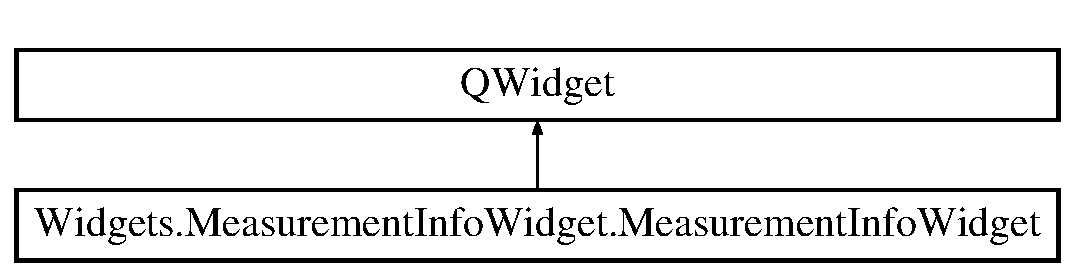
\includegraphics[height=2.000000cm]{classWidgets_1_1MeasurementInfoWidget_1_1MeasurementInfoWidget}
\end{center}
\end{figure}
\subsection*{Public Member Functions}
\begin{DoxyCompactItemize}
\item 
\hypertarget{classWidgets_1_1MeasurementInfoWidget_1_1MeasurementInfoWidget_a5cc553f810b6582d39c6a105c5f050c9}{def {\bfseries \-\_\-\-\_\-init\-\_\-\-\_\-}}\label{classWidgets_1_1MeasurementInfoWidget_1_1MeasurementInfoWidget_a5cc553f810b6582d39c6a105c5f050c9}

\end{DoxyCompactItemize}
\subsection*{Public Attributes}
\begin{DoxyCompactItemize}
\item 
\hypertarget{classWidgets_1_1MeasurementInfoWidget_1_1MeasurementInfoWidget_a6793251b040a8e67de81a3994366abee}{{\bfseries ui}}\label{classWidgets_1_1MeasurementInfoWidget_1_1MeasurementInfoWidget_a6793251b040a8e67de81a3994366abee}

\end{DoxyCompactItemize}


\subsection{Detailed Description}
\begin{DoxyVerb}Class for creating an info tab widget
\end{DoxyVerb}
 

The documentation for this class was generated from the following file\-:\begin{DoxyCompactItemize}
\item 
Widgets/Measurement\-Info\-Widget.\-py\end{DoxyCompactItemize}

\hypertarget{classModules_1_1Measurement_1_1Measurements}{\section{Modules.\-Measurement.\-Measurements Class Reference}
\label{classModules_1_1Measurement_1_1Measurements}\index{Modules.\-Measurement.\-Measurements@{Modules.\-Measurement.\-Measurements}}
}
\subsection*{Public Member Functions}
\begin{DoxyCompactItemize}
\item 
def \hyperlink{classModules_1_1Measurement_1_1Measurements_a7fd84aa1e23987dfab6ff6be8963d46b}{\-\_\-\-\_\-init\-\_\-\-\_\-}
\item 
def \hyperlink{classModules_1_1Measurement_1_1Measurements_abf24668677bfc6643a281dbee60ad6e6}{is\-\_\-empty}
\item 
\hypertarget{classModules_1_1Measurement_1_1Measurements_ae09e067353055563c7874b83cffe6900}{def {\bfseries get\-\_\-key\-\_\-value}}\label{classModules_1_1Measurement_1_1Measurements_ae09e067353055563c7874b83cffe6900}

\item 
def \hyperlink{classModules_1_1Measurement_1_1Measurements_af23574d8f8d6dc2390313022a39a06d0}{add\-\_\-measurement\-\_\-file}
\item 
def \hyperlink{classModules_1_1Measurement_1_1Measurements_a225559ff490f6291a7e82525cd08c836}{remove\-\_\-by\-\_\-tab\-\_\-id}
\end{DoxyCompactItemize}
\subsection*{Public Attributes}
\begin{DoxyCompactItemize}
\item 
\hypertarget{classModules_1_1Measurement_1_1Measurements_a06a95dd7297b64b43b1279e5fbd702f5}{{\bfseries project}}\label{classModules_1_1Measurement_1_1Measurements_a06a95dd7297b64b43b1279e5fbd702f5}

\item 
\hypertarget{classModules_1_1Measurement_1_1Measurements_a9b52a373e9f67d93778fc272b40aec6d}{{\bfseries measurements}}\label{classModules_1_1Measurement_1_1Measurements_a9b52a373e9f67d93778fc272b40aec6d}

\item 
\hypertarget{classModules_1_1Measurement_1_1Measurements_a9475a1a0676e96790473595bb8ba3707}{{\bfseries measuring\-\_\-unit\-\_\-settings}}\label{classModules_1_1Measurement_1_1Measurements_a9475a1a0676e96790473595bb8ba3707}

\item 
\hypertarget{classModules_1_1Measurement_1_1Measurements_a38139fdda46fc9fbc2a7c5ef097aa8bf}{{\bfseries default\-\_\-settings}}\label{classModules_1_1Measurement_1_1Measurements_a38139fdda46fc9fbc2a7c5ef097aa8bf}

\end{DoxyCompactItemize}


\subsection{Detailed Description}
\begin{DoxyVerb}Measurements class handles multiple measurements.
\end{DoxyVerb}
 

\subsection{Constructor \& Destructor Documentation}
\hypertarget{classModules_1_1Measurement_1_1Measurements_a7fd84aa1e23987dfab6ff6be8963d46b}{\index{Modules\-::\-Measurement\-::\-Measurements@{Modules\-::\-Measurement\-::\-Measurements}!\-\_\-\-\_\-init\-\_\-\-\_\-@{\-\_\-\-\_\-init\-\_\-\-\_\-}}
\index{\-\_\-\-\_\-init\-\_\-\-\_\-@{\-\_\-\-\_\-init\-\_\-\-\_\-}!Modules::Measurement::Measurements@{Modules\-::\-Measurement\-::\-Measurements}}
\subsubsection[{\-\_\-\-\_\-init\-\_\-\-\_\-}]{\setlength{\rightskip}{0pt plus 5cm}def Modules.\-Measurement.\-Measurements.\-\_\-\-\_\-init\-\_\-\-\_\- (
\begin{DoxyParamCaption}
\item[{}]{self, }
\item[{}]{project}
\end{DoxyParamCaption}
)}}\label{classModules_1_1Measurement_1_1Measurements_a7fd84aa1e23987dfab6ff6be8963d46b}
\begin{DoxyVerb}Inits measurements class.

Args:
    project: Project class object.
\end{DoxyVerb}
 

\subsection{Member Function Documentation}
\hypertarget{classModules_1_1Measurement_1_1Measurements_af23574d8f8d6dc2390313022a39a06d0}{\index{Modules\-::\-Measurement\-::\-Measurements@{Modules\-::\-Measurement\-::\-Measurements}!add\-\_\-measurement\-\_\-file@{add\-\_\-measurement\-\_\-file}}
\index{add\-\_\-measurement\-\_\-file@{add\-\_\-measurement\-\_\-file}!Modules::Measurement::Measurements@{Modules\-::\-Measurement\-::\-Measurements}}
\subsubsection[{add\-\_\-measurement\-\_\-file}]{\setlength{\rightskip}{0pt plus 5cm}def Modules.\-Measurement.\-Measurements.\-add\-\_\-measurement\-\_\-file (
\begin{DoxyParamCaption}
\item[{}]{self, }
\item[{}]{measurement\-\_\-file, }
\item[{}]{tab\-\_\-id}
\end{DoxyParamCaption}
)}}\label{classModules_1_1Measurement_1_1Measurements_af23574d8f8d6dc2390313022a39a06d0}
\begin{DoxyVerb}Add a new file to measurements.

Args:
    measurement_filepath: String representing file containing measurement 
                  data.
    tab_id: Integer representing identifier for measurement's tab.

Return:
    Returns new measurement or None if it wasn't added
\end{DoxyVerb}
 \hypertarget{classModules_1_1Measurement_1_1Measurements_abf24668677bfc6643a281dbee60ad6e6}{\index{Modules\-::\-Measurement\-::\-Measurements@{Modules\-::\-Measurement\-::\-Measurements}!is\-\_\-empty@{is\-\_\-empty}}
\index{is\-\_\-empty@{is\-\_\-empty}!Modules::Measurement::Measurements@{Modules\-::\-Measurement\-::\-Measurements}}
\subsubsection[{is\-\_\-empty}]{\setlength{\rightskip}{0pt plus 5cm}def Modules.\-Measurement.\-Measurements.\-is\-\_\-empty (
\begin{DoxyParamCaption}
\item[{}]{self}
\end{DoxyParamCaption}
)}}\label{classModules_1_1Measurement_1_1Measurements_abf24668677bfc6643a281dbee60ad6e6}
\begin{DoxyVerb}Check if there are any measurements.

Return:
    Returns True if there are no measurements currently in the 
    measurements object.
\end{DoxyVerb}
 \hypertarget{classModules_1_1Measurement_1_1Measurements_a225559ff490f6291a7e82525cd08c836}{\index{Modules\-::\-Measurement\-::\-Measurements@{Modules\-::\-Measurement\-::\-Measurements}!remove\-\_\-by\-\_\-tab\-\_\-id@{remove\-\_\-by\-\_\-tab\-\_\-id}}
\index{remove\-\_\-by\-\_\-tab\-\_\-id@{remove\-\_\-by\-\_\-tab\-\_\-id}!Modules::Measurement::Measurements@{Modules\-::\-Measurement\-::\-Measurements}}
\subsubsection[{remove\-\_\-by\-\_\-tab\-\_\-id}]{\setlength{\rightskip}{0pt plus 5cm}def Modules.\-Measurement.\-Measurements.\-remove\-\_\-by\-\_\-tab\-\_\-id (
\begin{DoxyParamCaption}
\item[{}]{self, }
\item[{}]{tab\-\_\-id}
\end{DoxyParamCaption}
)}}\label{classModules_1_1Measurement_1_1Measurements_a225559ff490f6291a7e82525cd08c836}
\begin{DoxyVerb}Removes measurement from measurements by tab id

Args:
    tab_id: Integer representing tab identifier.
\end{DoxyVerb}
 

The documentation for this class was generated from the following file\-:\begin{DoxyCompactItemize}
\item 
Modules/Measurement.\-py\end{DoxyCompactItemize}

\hypertarget{classWidgets_1_1MeasurementTabWidget_1_1MeasurementTabWidget}{\section{Widgets.\-Measurement\-Tab\-Widget.\-Measurement\-Tab\-Widget Class Reference}
\label{classWidgets_1_1MeasurementTabWidget_1_1MeasurementTabWidget}\index{Widgets.\-Measurement\-Tab\-Widget.\-Measurement\-Tab\-Widget@{Widgets.\-Measurement\-Tab\-Widget.\-Measurement\-Tab\-Widget}}
}
Inheritance diagram for Widgets.\-Measurement\-Tab\-Widget.\-Measurement\-Tab\-Widget\-:\begin{figure}[H]
\begin{center}
\leavevmode
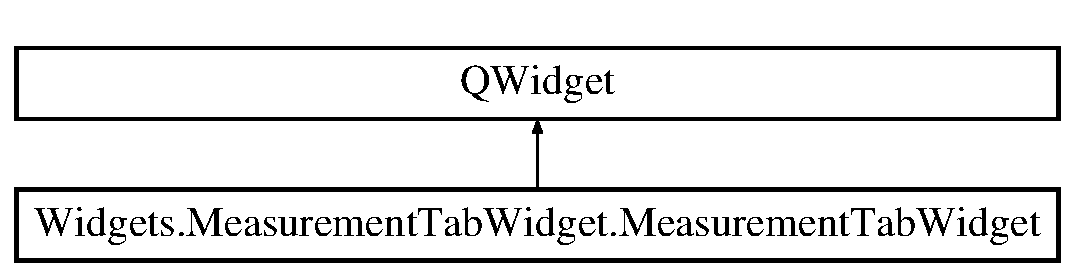
\includegraphics[height=2.000000cm]{classWidgets_1_1MeasurementTabWidget_1_1MeasurementTabWidget}
\end{center}
\end{figure}
\subsection*{Public Member Functions}
\begin{DoxyCompactItemize}
\item 
def \hyperlink{classWidgets_1_1MeasurementTabWidget_1_1MeasurementTabWidget_aee8d444727e46c8cced9fbf853419a39}{\-\_\-\-\_\-init\-\_\-\-\_\-}
\item 
def \hyperlink{classWidgets_1_1MeasurementTabWidget_1_1MeasurementTabWidget_aa070662ef900e9907610b36c28c8a490}{add\-\_\-widget}
\item 
def \hyperlink{classWidgets_1_1MeasurementTabWidget_1_1MeasurementTabWidget_a972a6411dbb7ca0f543988a9fbf61674}{add\-\_\-histogram}
\item 
def \hyperlink{classWidgets_1_1MeasurementTabWidget_1_1MeasurementTabWidget_ab12a0b756830705f4109088b33452387}{add\-\_\-log}
\item 
def \hyperlink{classWidgets_1_1MeasurementTabWidget_1_1MeasurementTabWidget_aa40815ca2f4ea199fac48d6c3efea900}{add\-\_\-\-U\-I\-\_\-logger}
\item 
def \hyperlink{classWidgets_1_1MeasurementTabWidget_1_1MeasurementTabWidget_a44ee930bec8552a41159fed591abf317}{check\-\_\-previous\-\_\-state\-\_\-files}
\item 
def \hyperlink{classWidgets_1_1MeasurementTabWidget_1_1MeasurementTabWidget_ab0ffed8501ddb2ca75ab043f5a20540b}{del\-\_\-widget}
\item 
def \hyperlink{classWidgets_1_1MeasurementTabWidget_1_1MeasurementTabWidget_a042148f7e08099d81b6b5886c9332789}{hide\-\_\-panel}
\item 
def \hyperlink{classWidgets_1_1MeasurementTabWidget_1_1MeasurementTabWidget_a51d34b697fe0f0d22cfe3fad148b6c8c}{make\-\_\-depth\-\_\-profile}
\item 
def \hyperlink{classWidgets_1_1MeasurementTabWidget_1_1MeasurementTabWidget_a8e2dfa5263df4845e53013cc345cf042}{make\-\_\-elemental\-\_\-losses}
\item 
def \hyperlink{classWidgets_1_1MeasurementTabWidget_1_1MeasurementTabWidget_a70ab9b1243c4cad761a5784c6e20b9e6}{make\-\_\-energy\-\_\-spectrum}
\item 
def \hyperlink{classWidgets_1_1MeasurementTabWidget_1_1MeasurementTabWidget_ae4adbb3c898d97c74718decf9951e0e3}{measurement\-\_\-save\-\_\-cuts}
\item 
def \hyperlink{classWidgets_1_1MeasurementTabWidget_1_1MeasurementTabWidget_a8fe4a059bd2edc9bf68779245d4371b4}{open\-\_\-measuring\-\_\-unit\-\_\-settings}
\item 
def \hyperlink{classWidgets_1_1MeasurementTabWidget_1_1MeasurementTabWidget_a55eecc37c804f503155b22a515d8bfaf}{open\-\_\-depth\-\_\-profile\-\_\-settings}
\item 
def \hyperlink{classWidgets_1_1MeasurementTabWidget_1_1MeasurementTabWidget_aac1139df5d6bd8e7b9f34662ada036db}{open\-\_\-calibration\-\_\-settings}
\item 
def \hyperlink{classWidgets_1_1MeasurementTabWidget_1_1MeasurementTabWidget_ab0f18c81b0023150e714a3860df83a59}{open\-\_\-depth\-\_\-profile}
\item 
def \hyperlink{classWidgets_1_1MeasurementTabWidget_1_1MeasurementTabWidget_a6451f850af1e0f13fd423ce374b1d04e}{open\-\_\-energy\-\_\-spectrum}
\item 
def \hyperlink{classWidgets_1_1MeasurementTabWidget_1_1MeasurementTabWidget_a4da1f4c408eda060c241483e9c0162a8}{open\-\_\-element\-\_\-losses}
\item 
def \hyperlink{classWidgets_1_1MeasurementTabWidget_1_1MeasurementTabWidget_a91a341576a00d9db7f66a7ffe8aba396}{toggle\-\_\-master\-\_\-button}
\end{DoxyCompactItemize}
\subsection*{Public Attributes}
\begin{DoxyCompactItemize}
\item 
\hypertarget{classWidgets_1_1MeasurementTabWidget_1_1MeasurementTabWidget_ac9a2279c774dad9d1f5c4469f6d1dd92}{{\bfseries tab\-\_\-id}}\label{classWidgets_1_1MeasurementTabWidget_1_1MeasurementTabWidget_ac9a2279c774dad9d1f5c4469f6d1dd92}

\item 
\hypertarget{classWidgets_1_1MeasurementTabWidget_1_1MeasurementTabWidget_a4839c9cd7d36566e7f1a1f09bae92986}{{\bfseries ui}}\label{classWidgets_1_1MeasurementTabWidget_1_1MeasurementTabWidget_a4839c9cd7d36566e7f1a1f09bae92986}

\item 
\hypertarget{classWidgets_1_1MeasurementTabWidget_1_1MeasurementTabWidget_a46f94d91ef21522a1a3e11eed9d2c933}{{\bfseries measurement}}\label{classWidgets_1_1MeasurementTabWidget_1_1MeasurementTabWidget_a46f94d91ef21522a1a3e11eed9d2c933}

\item 
\hypertarget{classWidgets_1_1MeasurementTabWidget_1_1MeasurementTabWidget_a58d1880902869ffbfeadf3a007da8844}{{\bfseries masses}}\label{classWidgets_1_1MeasurementTabWidget_1_1MeasurementTabWidget_a58d1880902869ffbfeadf3a007da8844}

\item 
\hypertarget{classWidgets_1_1MeasurementTabWidget_1_1MeasurementTabWidget_a433b1e7289229e7b5682cdf5e9459170}{{\bfseries icon\-\_\-manager}}\label{classWidgets_1_1MeasurementTabWidget_1_1MeasurementTabWidget_a433b1e7289229e7b5682cdf5e9459170}

\item 
\hypertarget{classWidgets_1_1MeasurementTabWidget_1_1MeasurementTabWidget_a1cfd25be0f10c70c6dce6c02f05a8b10}{{\bfseries histogram}}\label{classWidgets_1_1MeasurementTabWidget_1_1MeasurementTabWidget_a1cfd25be0f10c70c6dce6c02f05a8b10}

\item 
\hypertarget{classWidgets_1_1MeasurementTabWidget_1_1MeasurementTabWidget_a4ddd94cdbae016a89568b619d4b625d1}{{\bfseries elemental\-\_\-losses\-\_\-widget}}\label{classWidgets_1_1MeasurementTabWidget_1_1MeasurementTabWidget_a4ddd94cdbae016a89568b619d4b625d1}

\item 
\hypertarget{classWidgets_1_1MeasurementTabWidget_1_1MeasurementTabWidget_afc2d265671067e07f9b391f59e41f5b4}{{\bfseries energy\-\_\-spectrum\-\_\-widget}}\label{classWidgets_1_1MeasurementTabWidget_1_1MeasurementTabWidget_afc2d265671067e07f9b391f59e41f5b4}

\item 
\hypertarget{classWidgets_1_1MeasurementTabWidget_1_1MeasurementTabWidget_ab9b27989a0ca97792a551aff950abd27}{{\bfseries depth\-\_\-profile\-\_\-widget}}\label{classWidgets_1_1MeasurementTabWidget_1_1MeasurementTabWidget_ab9b27989a0ca97792a551aff950abd27}

\item 
\hypertarget{classWidgets_1_1MeasurementTabWidget_1_1MeasurementTabWidget_a972d604db691d5df0e926c7d73e8627a}{{\bfseries data\-\_\-loaded}}\label{classWidgets_1_1MeasurementTabWidget_1_1MeasurementTabWidget_a972d604db691d5df0e926c7d73e8627a}

\item 
\hypertarget{classWidgets_1_1MeasurementTabWidget_1_1MeasurementTabWidget_abac09b9a5299b26137cdf82c3b2428aa}{{\bfseries panel\-\_\-shown}}\label{classWidgets_1_1MeasurementTabWidget_1_1MeasurementTabWidget_abac09b9a5299b26137cdf82c3b2428aa}

\item 
\hypertarget{classWidgets_1_1MeasurementTabWidget_1_1MeasurementTabWidget_a442ad52314a8ef4a886f838909eac71b}{{\bfseries log}}\label{classWidgets_1_1MeasurementTabWidget_1_1MeasurementTabWidget_a442ad52314a8ef4a886f838909eac71b}

\end{DoxyCompactItemize}
\subsection*{Static Public Attributes}
\begin{DoxyCompactItemize}
\item 
\hypertarget{classWidgets_1_1MeasurementTabWidget_1_1MeasurementTabWidget_aab78674401a0a766e823abbb6d208cbd}{tuple {\bfseries issue\-Master} = Qt\-Core.\-pyqt\-Signal()}\label{classWidgets_1_1MeasurementTabWidget_1_1MeasurementTabWidget_aab78674401a0a766e823abbb6d208cbd}

\end{DoxyCompactItemize}


\subsection{Detailed Description}
\begin{DoxyVerb}Tab widget where measurement stuff is added.
\end{DoxyVerb}
 

\subsection{Constructor \& Destructor Documentation}
\hypertarget{classWidgets_1_1MeasurementTabWidget_1_1MeasurementTabWidget_aee8d444727e46c8cced9fbf853419a39}{\index{Widgets\-::\-Measurement\-Tab\-Widget\-::\-Measurement\-Tab\-Widget@{Widgets\-::\-Measurement\-Tab\-Widget\-::\-Measurement\-Tab\-Widget}!\-\_\-\-\_\-init\-\_\-\-\_\-@{\-\_\-\-\_\-init\-\_\-\-\_\-}}
\index{\-\_\-\-\_\-init\-\_\-\-\_\-@{\-\_\-\-\_\-init\-\_\-\-\_\-}!Widgets::MeasurementTabWidget::MeasurementTabWidget@{Widgets\-::\-Measurement\-Tab\-Widget\-::\-Measurement\-Tab\-Widget}}
\subsubsection[{\-\_\-\-\_\-init\-\_\-\-\_\-}]{\setlength{\rightskip}{0pt plus 5cm}def Widgets.\-Measurement\-Tab\-Widget.\-Measurement\-Tab\-Widget.\-\_\-\-\_\-init\-\_\-\-\_\- (
\begin{DoxyParamCaption}
\item[{}]{self, }
\item[{}]{tab\-\_\-id, }
\item[{}]{measurement, }
\item[{}]{masses, }
\item[{}]{icon\-\_\-manager}
\end{DoxyParamCaption}
)}}\label{classWidgets_1_1MeasurementTabWidget_1_1MeasurementTabWidget_aee8d444727e46c8cced9fbf853419a39}
\begin{DoxyVerb}Init measurement tab class.

Args:
    tab_id: An integer representing ID of the tabwidget.
    measurement: A measurement class object.
    masses: A masses class object.
    icon_manager: An iconmanager class object.
\end{DoxyVerb}
 

\subsection{Member Function Documentation}
\hypertarget{classWidgets_1_1MeasurementTabWidget_1_1MeasurementTabWidget_a972a6411dbb7ca0f543988a9fbf61674}{\index{Widgets\-::\-Measurement\-Tab\-Widget\-::\-Measurement\-Tab\-Widget@{Widgets\-::\-Measurement\-Tab\-Widget\-::\-Measurement\-Tab\-Widget}!add\-\_\-histogram@{add\-\_\-histogram}}
\index{add\-\_\-histogram@{add\-\_\-histogram}!Widgets::MeasurementTabWidget::MeasurementTabWidget@{Widgets\-::\-Measurement\-Tab\-Widget\-::\-Measurement\-Tab\-Widget}}
\subsubsection[{add\-\_\-histogram}]{\setlength{\rightskip}{0pt plus 5cm}def Widgets.\-Measurement\-Tab\-Widget.\-Measurement\-Tab\-Widget.\-add\-\_\-histogram (
\begin{DoxyParamCaption}
\item[{}]{self}
\end{DoxyParamCaption}
)}}\label{classWidgets_1_1MeasurementTabWidget_1_1MeasurementTabWidget_a972a6411dbb7ca0f543988a9fbf61674}
\begin{DoxyVerb}Adds ToF-E histogram into tab if it doesn't have one already.
\end{DoxyVerb}
 \hypertarget{classWidgets_1_1MeasurementTabWidget_1_1MeasurementTabWidget_ab12a0b756830705f4109088b33452387}{\index{Widgets\-::\-Measurement\-Tab\-Widget\-::\-Measurement\-Tab\-Widget@{Widgets\-::\-Measurement\-Tab\-Widget\-::\-Measurement\-Tab\-Widget}!add\-\_\-log@{add\-\_\-log}}
\index{add\-\_\-log@{add\-\_\-log}!Widgets::MeasurementTabWidget::MeasurementTabWidget@{Widgets\-::\-Measurement\-Tab\-Widget\-::\-Measurement\-Tab\-Widget}}
\subsubsection[{add\-\_\-log}]{\setlength{\rightskip}{0pt plus 5cm}def Widgets.\-Measurement\-Tab\-Widget.\-Measurement\-Tab\-Widget.\-add\-\_\-log (
\begin{DoxyParamCaption}
\item[{}]{self}
\end{DoxyParamCaption}
)}}\label{classWidgets_1_1MeasurementTabWidget_1_1MeasurementTabWidget_ab12a0b756830705f4109088b33452387}
\begin{DoxyVerb}Add the measurement log to measurement tab widget.

Checks also if there's already some logging for this measurement and appends 
the text field of the user interface with this log.
\end{DoxyVerb}
 \hypertarget{classWidgets_1_1MeasurementTabWidget_1_1MeasurementTabWidget_aa40815ca2f4ea199fac48d6c3efea900}{\index{Widgets\-::\-Measurement\-Tab\-Widget\-::\-Measurement\-Tab\-Widget@{Widgets\-::\-Measurement\-Tab\-Widget\-::\-Measurement\-Tab\-Widget}!add\-\_\-\-U\-I\-\_\-logger@{add\-\_\-\-U\-I\-\_\-logger}}
\index{add\-\_\-\-U\-I\-\_\-logger@{add\-\_\-\-U\-I\-\_\-logger}!Widgets::MeasurementTabWidget::MeasurementTabWidget@{Widgets\-::\-Measurement\-Tab\-Widget\-::\-Measurement\-Tab\-Widget}}
\subsubsection[{add\-\_\-\-U\-I\-\_\-logger}]{\setlength{\rightskip}{0pt plus 5cm}def Widgets.\-Measurement\-Tab\-Widget.\-Measurement\-Tab\-Widget.\-add\-\_\-\-U\-I\-\_\-logger (
\begin{DoxyParamCaption}
\item[{}]{self, }
\item[{}]{log\-\_\-widget}
\end{DoxyParamCaption}
)}}\label{classWidgets_1_1MeasurementTabWidget_1_1MeasurementTabWidget_aa40815ca2f4ea199fac48d6c3efea900}
\begin{DoxyVerb}Adds handlers to measurement logger so the logger can log the events to 
the user interface too.

log_widget specifies which ui element will handle the logging. That should 
be the one which is added to this MeasurementTabWidget.
\end{DoxyVerb}
 \hypertarget{classWidgets_1_1MeasurementTabWidget_1_1MeasurementTabWidget_aa070662ef900e9907610b36c28c8a490}{\index{Widgets\-::\-Measurement\-Tab\-Widget\-::\-Measurement\-Tab\-Widget@{Widgets\-::\-Measurement\-Tab\-Widget\-::\-Measurement\-Tab\-Widget}!add\-\_\-widget@{add\-\_\-widget}}
\index{add\-\_\-widget@{add\-\_\-widget}!Widgets::MeasurementTabWidget::MeasurementTabWidget@{Widgets\-::\-Measurement\-Tab\-Widget\-::\-Measurement\-Tab\-Widget}}
\subsubsection[{add\-\_\-widget}]{\setlength{\rightskip}{0pt plus 5cm}def Widgets.\-Measurement\-Tab\-Widget.\-Measurement\-Tab\-Widget.\-add\-\_\-widget (
\begin{DoxyParamCaption}
\item[{}]{self, }
\item[{}]{widget, }
\item[{}]{minimized = {\ttfamily None}, }
\item[{}]{has\-\_\-close\-\_\-button = {\ttfamily True}, }
\item[{}]{icon = {\ttfamily None}}
\end{DoxyParamCaption}
)}}\label{classWidgets_1_1MeasurementTabWidget_1_1MeasurementTabWidget_aa070662ef900e9907610b36c28c8a490}
\begin{DoxyVerb}Adds a new widget to current (measurement) tab.

Args:
    widget: QWidget to be added into measurement tab widget.
    minimized: Boolean representing if widget should be minimized.
    icon: QtGui.QIcon for the subwindow. 
\end{DoxyVerb}
 \hypertarget{classWidgets_1_1MeasurementTabWidget_1_1MeasurementTabWidget_a44ee930bec8552a41159fed591abf317}{\index{Widgets\-::\-Measurement\-Tab\-Widget\-::\-Measurement\-Tab\-Widget@{Widgets\-::\-Measurement\-Tab\-Widget\-::\-Measurement\-Tab\-Widget}!check\-\_\-previous\-\_\-state\-\_\-files@{check\-\_\-previous\-\_\-state\-\_\-files}}
\index{check\-\_\-previous\-\_\-state\-\_\-files@{check\-\_\-previous\-\_\-state\-\_\-files}!Widgets::MeasurementTabWidget::MeasurementTabWidget@{Widgets\-::\-Measurement\-Tab\-Widget\-::\-Measurement\-Tab\-Widget}}
\subsubsection[{check\-\_\-previous\-\_\-state\-\_\-files}]{\setlength{\rightskip}{0pt plus 5cm}def Widgets.\-Measurement\-Tab\-Widget.\-Measurement\-Tab\-Widget.\-check\-\_\-previous\-\_\-state\-\_\-files (
\begin{DoxyParamCaption}
\item[{}]{self, }
\item[{}]{progress\-\_\-bar = {\ttfamily {\bf Null}()}, }
\item[{}]{directory = {\ttfamily None}}
\end{DoxyParamCaption}
)}}\label{classWidgets_1_1MeasurementTabWidget_1_1MeasurementTabWidget_a44ee930bec8552a41159fed591abf317}
\begin{DoxyVerb}Check if saved state for Elemental Losses, Energy Spectrum or Depth 
Profile exists. If yes, load them also.

Args:
    progress_bar: A QtWidgets.QProgressBar where loading of previous
          graph can be shown.
\end{DoxyVerb}
 \hypertarget{classWidgets_1_1MeasurementTabWidget_1_1MeasurementTabWidget_ab0ffed8501ddb2ca75ab043f5a20540b}{\index{Widgets\-::\-Measurement\-Tab\-Widget\-::\-Measurement\-Tab\-Widget@{Widgets\-::\-Measurement\-Tab\-Widget\-::\-Measurement\-Tab\-Widget}!del\-\_\-widget@{del\-\_\-widget}}
\index{del\-\_\-widget@{del\-\_\-widget}!Widgets::MeasurementTabWidget::MeasurementTabWidget@{Widgets\-::\-Measurement\-Tab\-Widget\-::\-Measurement\-Tab\-Widget}}
\subsubsection[{del\-\_\-widget}]{\setlength{\rightskip}{0pt plus 5cm}def Widgets.\-Measurement\-Tab\-Widget.\-Measurement\-Tab\-Widget.\-del\-\_\-widget (
\begin{DoxyParamCaption}
\item[{}]{self, }
\item[{}]{widget}
\end{DoxyParamCaption}
)}}\label{classWidgets_1_1MeasurementTabWidget_1_1MeasurementTabWidget_ab0ffed8501ddb2ca75ab043f5a20540b}
\begin{DoxyVerb}Delete a widget from current (measurement) tab.

Args:
    widget: QWidget to be removed.
\end{DoxyVerb}
 \hypertarget{classWidgets_1_1MeasurementTabWidget_1_1MeasurementTabWidget_a042148f7e08099d81b6b5886c9332789}{\index{Widgets\-::\-Measurement\-Tab\-Widget\-::\-Measurement\-Tab\-Widget@{Widgets\-::\-Measurement\-Tab\-Widget\-::\-Measurement\-Tab\-Widget}!hide\-\_\-panel@{hide\-\_\-panel}}
\index{hide\-\_\-panel@{hide\-\_\-panel}!Widgets::MeasurementTabWidget::MeasurementTabWidget@{Widgets\-::\-Measurement\-Tab\-Widget\-::\-Measurement\-Tab\-Widget}}
\subsubsection[{hide\-\_\-panel}]{\setlength{\rightskip}{0pt plus 5cm}def Widgets.\-Measurement\-Tab\-Widget.\-Measurement\-Tab\-Widget.\-hide\-\_\-panel (
\begin{DoxyParamCaption}
\item[{}]{self, }
\item[{}]{enable\-\_\-hide = {\ttfamily None}}
\end{DoxyParamCaption}
)}}\label{classWidgets_1_1MeasurementTabWidget_1_1MeasurementTabWidget_a042148f7e08099d81b6b5886c9332789}
\begin{DoxyVerb}Sets the frame (including all the tool buttons) visible.

Args:
    enable_hide: If True, sets the frame visible and vice versa. 
         If not given, sets the frame visible or hidden 
         depending its previous state.
\end{DoxyVerb}
 \hypertarget{classWidgets_1_1MeasurementTabWidget_1_1MeasurementTabWidget_a51d34b697fe0f0d22cfe3fad148b6c8c}{\index{Widgets\-::\-Measurement\-Tab\-Widget\-::\-Measurement\-Tab\-Widget@{Widgets\-::\-Measurement\-Tab\-Widget\-::\-Measurement\-Tab\-Widget}!make\-\_\-depth\-\_\-profile@{make\-\_\-depth\-\_\-profile}}
\index{make\-\_\-depth\-\_\-profile@{make\-\_\-depth\-\_\-profile}!Widgets::MeasurementTabWidget::MeasurementTabWidget@{Widgets\-::\-Measurement\-Tab\-Widget\-::\-Measurement\-Tab\-Widget}}
\subsubsection[{make\-\_\-depth\-\_\-profile}]{\setlength{\rightskip}{0pt plus 5cm}def Widgets.\-Measurement\-Tab\-Widget.\-Measurement\-Tab\-Widget.\-make\-\_\-depth\-\_\-profile (
\begin{DoxyParamCaption}
\item[{}]{self, }
\item[{}]{directory, }
\item[{}]{name}
\end{DoxyParamCaption}
)}}\label{classWidgets_1_1MeasurementTabWidget_1_1MeasurementTabWidget_a51d34b697fe0f0d22cfe3fad148b6c8c}
\begin{DoxyVerb}Make depth profile from loaded lines from saved file.

Args:
    directory: A string representing directory.
    name: A string representing measurement's name.
\end{DoxyVerb}
 \hypertarget{classWidgets_1_1MeasurementTabWidget_1_1MeasurementTabWidget_a8e2dfa5263df4845e53013cc345cf042}{\index{Widgets\-::\-Measurement\-Tab\-Widget\-::\-Measurement\-Tab\-Widget@{Widgets\-::\-Measurement\-Tab\-Widget\-::\-Measurement\-Tab\-Widget}!make\-\_\-elemental\-\_\-losses@{make\-\_\-elemental\-\_\-losses}}
\index{make\-\_\-elemental\-\_\-losses@{make\-\_\-elemental\-\_\-losses}!Widgets::MeasurementTabWidget::MeasurementTabWidget@{Widgets\-::\-Measurement\-Tab\-Widget\-::\-Measurement\-Tab\-Widget}}
\subsubsection[{make\-\_\-elemental\-\_\-losses}]{\setlength{\rightskip}{0pt plus 5cm}def Widgets.\-Measurement\-Tab\-Widget.\-Measurement\-Tab\-Widget.\-make\-\_\-elemental\-\_\-losses (
\begin{DoxyParamCaption}
\item[{}]{self, }
\item[{}]{directory, }
\item[{}]{name}
\end{DoxyParamCaption}
)}}\label{classWidgets_1_1MeasurementTabWidget_1_1MeasurementTabWidget_a8e2dfa5263df4845e53013cc345cf042}
\begin{DoxyVerb}Make elemental losses from loaded lines from saved file.

Args:
    directory: A string representing directory.
    name: A string representing measurement's name.
\end{DoxyVerb}
 \hypertarget{classWidgets_1_1MeasurementTabWidget_1_1MeasurementTabWidget_a70ab9b1243c4cad761a5784c6e20b9e6}{\index{Widgets\-::\-Measurement\-Tab\-Widget\-::\-Measurement\-Tab\-Widget@{Widgets\-::\-Measurement\-Tab\-Widget\-::\-Measurement\-Tab\-Widget}!make\-\_\-energy\-\_\-spectrum@{make\-\_\-energy\-\_\-spectrum}}
\index{make\-\_\-energy\-\_\-spectrum@{make\-\_\-energy\-\_\-spectrum}!Widgets::MeasurementTabWidget::MeasurementTabWidget@{Widgets\-::\-Measurement\-Tab\-Widget\-::\-Measurement\-Tab\-Widget}}
\subsubsection[{make\-\_\-energy\-\_\-spectrum}]{\setlength{\rightskip}{0pt plus 5cm}def Widgets.\-Measurement\-Tab\-Widget.\-Measurement\-Tab\-Widget.\-make\-\_\-energy\-\_\-spectrum (
\begin{DoxyParamCaption}
\item[{}]{self, }
\item[{}]{directory, }
\item[{}]{name}
\end{DoxyParamCaption}
)}}\label{classWidgets_1_1MeasurementTabWidget_1_1MeasurementTabWidget_a70ab9b1243c4cad761a5784c6e20b9e6}
\begin{DoxyVerb}Make energy spectrum from loaded lines from saved file.

Args:
    directory: A string representing directory.
    name: A string representing measurement's name.
\end{DoxyVerb}
 \hypertarget{classWidgets_1_1MeasurementTabWidget_1_1MeasurementTabWidget_ae4adbb3c898d97c74718decf9951e0e3}{\index{Widgets\-::\-Measurement\-Tab\-Widget\-::\-Measurement\-Tab\-Widget@{Widgets\-::\-Measurement\-Tab\-Widget\-::\-Measurement\-Tab\-Widget}!measurement\-\_\-save\-\_\-cuts@{measurement\-\_\-save\-\_\-cuts}}
\index{measurement\-\_\-save\-\_\-cuts@{measurement\-\_\-save\-\_\-cuts}!Widgets::MeasurementTabWidget::MeasurementTabWidget@{Widgets\-::\-Measurement\-Tab\-Widget\-::\-Measurement\-Tab\-Widget}}
\subsubsection[{measurement\-\_\-save\-\_\-cuts}]{\setlength{\rightskip}{0pt plus 5cm}def Widgets.\-Measurement\-Tab\-Widget.\-Measurement\-Tab\-Widget.\-measurement\-\_\-save\-\_\-cuts (
\begin{DoxyParamCaption}
\item[{}]{self}
\end{DoxyParamCaption}
)}}\label{classWidgets_1_1MeasurementTabWidget_1_1MeasurementTabWidget_ae4adbb3c898d97c74718decf9951e0e3}
\begin{DoxyVerb}Save measurement selections to cut files.
\end{DoxyVerb}
 \hypertarget{classWidgets_1_1MeasurementTabWidget_1_1MeasurementTabWidget_aac1139df5d6bd8e7b9f34662ada036db}{\index{Widgets\-::\-Measurement\-Tab\-Widget\-::\-Measurement\-Tab\-Widget@{Widgets\-::\-Measurement\-Tab\-Widget\-::\-Measurement\-Tab\-Widget}!open\-\_\-calibration\-\_\-settings@{open\-\_\-calibration\-\_\-settings}}
\index{open\-\_\-calibration\-\_\-settings@{open\-\_\-calibration\-\_\-settings}!Widgets::MeasurementTabWidget::MeasurementTabWidget@{Widgets\-::\-Measurement\-Tab\-Widget\-::\-Measurement\-Tab\-Widget}}
\subsubsection[{open\-\_\-calibration\-\_\-settings}]{\setlength{\rightskip}{0pt plus 5cm}def Widgets.\-Measurement\-Tab\-Widget.\-Measurement\-Tab\-Widget.\-open\-\_\-calibration\-\_\-settings (
\begin{DoxyParamCaption}
\item[{}]{self}
\end{DoxyParamCaption}
)}}\label{classWidgets_1_1MeasurementTabWidget_1_1MeasurementTabWidget_aac1139df5d6bd8e7b9f34662ada036db}
\begin{DoxyVerb}Opens calibration settings dialog.
\end{DoxyVerb}
 \hypertarget{classWidgets_1_1MeasurementTabWidget_1_1MeasurementTabWidget_ab0f18c81b0023150e714a3860df83a59}{\index{Widgets\-::\-Measurement\-Tab\-Widget\-::\-Measurement\-Tab\-Widget@{Widgets\-::\-Measurement\-Tab\-Widget\-::\-Measurement\-Tab\-Widget}!open\-\_\-depth\-\_\-profile@{open\-\_\-depth\-\_\-profile}}
\index{open\-\_\-depth\-\_\-profile@{open\-\_\-depth\-\_\-profile}!Widgets::MeasurementTabWidget::MeasurementTabWidget@{Widgets\-::\-Measurement\-Tab\-Widget\-::\-Measurement\-Tab\-Widget}}
\subsubsection[{open\-\_\-depth\-\_\-profile}]{\setlength{\rightskip}{0pt plus 5cm}def Widgets.\-Measurement\-Tab\-Widget.\-Measurement\-Tab\-Widget.\-open\-\_\-depth\-\_\-profile (
\begin{DoxyParamCaption}
\item[{}]{self, }
\item[{}]{parent}
\end{DoxyParamCaption}
)}}\label{classWidgets_1_1MeasurementTabWidget_1_1MeasurementTabWidget_ab0f18c81b0023150e714a3860df83a59}
\begin{DoxyVerb}Opens depth profile dialog.

Args:
    parent: MeasurementTabWidget
\end{DoxyVerb}
 \hypertarget{classWidgets_1_1MeasurementTabWidget_1_1MeasurementTabWidget_a55eecc37c804f503155b22a515d8bfaf}{\index{Widgets\-::\-Measurement\-Tab\-Widget\-::\-Measurement\-Tab\-Widget@{Widgets\-::\-Measurement\-Tab\-Widget\-::\-Measurement\-Tab\-Widget}!open\-\_\-depth\-\_\-profile\-\_\-settings@{open\-\_\-depth\-\_\-profile\-\_\-settings}}
\index{open\-\_\-depth\-\_\-profile\-\_\-settings@{open\-\_\-depth\-\_\-profile\-\_\-settings}!Widgets::MeasurementTabWidget::MeasurementTabWidget@{Widgets\-::\-Measurement\-Tab\-Widget\-::\-Measurement\-Tab\-Widget}}
\subsubsection[{open\-\_\-depth\-\_\-profile\-\_\-settings}]{\setlength{\rightskip}{0pt plus 5cm}def Widgets.\-Measurement\-Tab\-Widget.\-Measurement\-Tab\-Widget.\-open\-\_\-depth\-\_\-profile\-\_\-settings (
\begin{DoxyParamCaption}
\item[{}]{self}
\end{DoxyParamCaption}
)}}\label{classWidgets_1_1MeasurementTabWidget_1_1MeasurementTabWidget_a55eecc37c804f503155b22a515d8bfaf}
\begin{DoxyVerb}Opens depth profile settings dialog.
\end{DoxyVerb}
 \hypertarget{classWidgets_1_1MeasurementTabWidget_1_1MeasurementTabWidget_a4da1f4c408eda060c241483e9c0162a8}{\index{Widgets\-::\-Measurement\-Tab\-Widget\-::\-Measurement\-Tab\-Widget@{Widgets\-::\-Measurement\-Tab\-Widget\-::\-Measurement\-Tab\-Widget}!open\-\_\-element\-\_\-losses@{open\-\_\-element\-\_\-losses}}
\index{open\-\_\-element\-\_\-losses@{open\-\_\-element\-\_\-losses}!Widgets::MeasurementTabWidget::MeasurementTabWidget@{Widgets\-::\-Measurement\-Tab\-Widget\-::\-Measurement\-Tab\-Widget}}
\subsubsection[{open\-\_\-element\-\_\-losses}]{\setlength{\rightskip}{0pt plus 5cm}def Widgets.\-Measurement\-Tab\-Widget.\-Measurement\-Tab\-Widget.\-open\-\_\-element\-\_\-losses (
\begin{DoxyParamCaption}
\item[{}]{self, }
\item[{}]{parent}
\end{DoxyParamCaption}
)}}\label{classWidgets_1_1MeasurementTabWidget_1_1MeasurementTabWidget_a4da1f4c408eda060c241483e9c0162a8}
\begin{DoxyVerb}Opens element losses dialog.

Args:
    parent: MeasurementTabWidget
\end{DoxyVerb}
 \hypertarget{classWidgets_1_1MeasurementTabWidget_1_1MeasurementTabWidget_a6451f850af1e0f13fd423ce374b1d04e}{\index{Widgets\-::\-Measurement\-Tab\-Widget\-::\-Measurement\-Tab\-Widget@{Widgets\-::\-Measurement\-Tab\-Widget\-::\-Measurement\-Tab\-Widget}!open\-\_\-energy\-\_\-spectrum@{open\-\_\-energy\-\_\-spectrum}}
\index{open\-\_\-energy\-\_\-spectrum@{open\-\_\-energy\-\_\-spectrum}!Widgets::MeasurementTabWidget::MeasurementTabWidget@{Widgets\-::\-Measurement\-Tab\-Widget\-::\-Measurement\-Tab\-Widget}}
\subsubsection[{open\-\_\-energy\-\_\-spectrum}]{\setlength{\rightskip}{0pt plus 5cm}def Widgets.\-Measurement\-Tab\-Widget.\-Measurement\-Tab\-Widget.\-open\-\_\-energy\-\_\-spectrum (
\begin{DoxyParamCaption}
\item[{}]{self, }
\item[{}]{parent}
\end{DoxyParamCaption}
)}}\label{classWidgets_1_1MeasurementTabWidget_1_1MeasurementTabWidget_a6451f850af1e0f13fd423ce374b1d04e}
\begin{DoxyVerb}Opens energy spectrum dialog.

Args:
    parent: MeasurementTabWidget
\end{DoxyVerb}
 \hypertarget{classWidgets_1_1MeasurementTabWidget_1_1MeasurementTabWidget_a8fe4a059bd2edc9bf68779245d4371b4}{\index{Widgets\-::\-Measurement\-Tab\-Widget\-::\-Measurement\-Tab\-Widget@{Widgets\-::\-Measurement\-Tab\-Widget\-::\-Measurement\-Tab\-Widget}!open\-\_\-measuring\-\_\-unit\-\_\-settings@{open\-\_\-measuring\-\_\-unit\-\_\-settings}}
\index{open\-\_\-measuring\-\_\-unit\-\_\-settings@{open\-\_\-measuring\-\_\-unit\-\_\-settings}!Widgets::MeasurementTabWidget::MeasurementTabWidget@{Widgets\-::\-Measurement\-Tab\-Widget\-::\-Measurement\-Tab\-Widget}}
\subsubsection[{open\-\_\-measuring\-\_\-unit\-\_\-settings}]{\setlength{\rightskip}{0pt plus 5cm}def Widgets.\-Measurement\-Tab\-Widget.\-Measurement\-Tab\-Widget.\-open\-\_\-measuring\-\_\-unit\-\_\-settings (
\begin{DoxyParamCaption}
\item[{}]{self}
\end{DoxyParamCaption}
)}}\label{classWidgets_1_1MeasurementTabWidget_1_1MeasurementTabWidget_a8fe4a059bd2edc9bf68779245d4371b4}
\begin{DoxyVerb}Opens measurement settings dialog.
\end{DoxyVerb}
 \hypertarget{classWidgets_1_1MeasurementTabWidget_1_1MeasurementTabWidget_a91a341576a00d9db7f66a7ffe8aba396}{\index{Widgets\-::\-Measurement\-Tab\-Widget\-::\-Measurement\-Tab\-Widget@{Widgets\-::\-Measurement\-Tab\-Widget\-::\-Measurement\-Tab\-Widget}!toggle\-\_\-master\-\_\-button@{toggle\-\_\-master\-\_\-button}}
\index{toggle\-\_\-master\-\_\-button@{toggle\-\_\-master\-\_\-button}!Widgets::MeasurementTabWidget::MeasurementTabWidget@{Widgets\-::\-Measurement\-Tab\-Widget\-::\-Measurement\-Tab\-Widget}}
\subsubsection[{toggle\-\_\-master\-\_\-button}]{\setlength{\rightskip}{0pt plus 5cm}def Widgets.\-Measurement\-Tab\-Widget.\-Measurement\-Tab\-Widget.\-toggle\-\_\-master\-\_\-button (
\begin{DoxyParamCaption}
\item[{}]{self}
\end{DoxyParamCaption}
)}}\label{classWidgets_1_1MeasurementTabWidget_1_1MeasurementTabWidget_a91a341576a00d9db7f66a7ffe8aba396}
\begin{DoxyVerb}Toggle enabled state of the master measurement button in the
measurementtabwidget.
\end{DoxyVerb}
 

The documentation for this class was generated from the following file\-:\begin{DoxyCompactItemize}
\item 
Widgets/Measurement\-Tab\-Widget.\-py\end{DoxyCompactItemize}

\hypertarget{classDialogs_1_1MeasurementSettingsDialogs_1_1MeasurementUnitSettings}{\section{Dialogs.\-Measurement\-Settings\-Dialogs.\-Measurement\-Unit\-Settings Class Reference}
\label{classDialogs_1_1MeasurementSettingsDialogs_1_1MeasurementUnitSettings}\index{Dialogs.\-Measurement\-Settings\-Dialogs.\-Measurement\-Unit\-Settings@{Dialogs.\-Measurement\-Settings\-Dialogs.\-Measurement\-Unit\-Settings}}
}
Inheritance diagram for Dialogs.\-Measurement\-Settings\-Dialogs.\-Measurement\-Unit\-Settings\-:\begin{figure}[H]
\begin{center}
\leavevmode
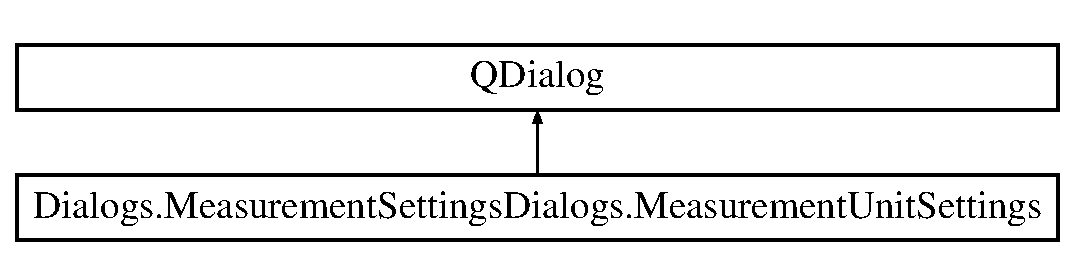
\includegraphics[height=2.000000cm]{classDialogs_1_1MeasurementSettingsDialogs_1_1MeasurementUnitSettings}
\end{center}
\end{figure}
\subsection*{Public Member Functions}
\begin{DoxyCompactItemize}
\item 
def \hyperlink{classDialogs_1_1MeasurementSettingsDialogs_1_1MeasurementUnitSettings_aaa4654df0caa128cb479935495053e5b}{\-\_\-\-\_\-init\-\_\-\-\_\-}
\item 
def \hyperlink{classDialogs_1_1MeasurementSettingsDialogs_1_1MeasurementUnitSettings_a3b51ca16f364d8eb3b38b2c69ca052eb}{update\-\_\-and\-\_\-close\-\_\-settings}
\end{DoxyCompactItemize}
\subsection*{Public Attributes}
\begin{DoxyCompactItemize}
\item 
\hypertarget{classDialogs_1_1MeasurementSettingsDialogs_1_1MeasurementUnitSettings_a1e3a3d6361b397849c704733b03fb6e0}{{\bfseries ui}}\label{classDialogs_1_1MeasurementSettingsDialogs_1_1MeasurementUnitSettings_a1e3a3d6361b397849c704733b03fb6e0}

\item 
\hypertarget{classDialogs_1_1MeasurementSettingsDialogs_1_1MeasurementUnitSettings_a12cbb8f66bf81b660f6f17f06f9b4ef5}{{\bfseries masses}}\label{classDialogs_1_1MeasurementSettingsDialogs_1_1MeasurementUnitSettings_a12cbb8f66bf81b660f6f17f06f9b4ef5}

\item 
\hypertarget{classDialogs_1_1MeasurementSettingsDialogs_1_1MeasurementUnitSettings_a44bf94de63f94f2f1e4b68db56164e9d}{{\bfseries project\-\_\-settings}}\label{classDialogs_1_1MeasurementSettingsDialogs_1_1MeasurementUnitSettings_a44bf94de63f94f2f1e4b68db56164e9d}

\item 
\hypertarget{classDialogs_1_1MeasurementSettingsDialogs_1_1MeasurementUnitSettings_af942f9371b9f5220f6dc4bf1bca0888f}{{\bfseries default\-\_\-folder}}\label{classDialogs_1_1MeasurementSettingsDialogs_1_1MeasurementUnitSettings_af942f9371b9f5220f6dc4bf1bca0888f}

\item 
\hypertarget{classDialogs_1_1MeasurementSettingsDialogs_1_1MeasurementUnitSettings_a3fa3c3431b066068acd4ba6525c0dd93}{{\bfseries settings}}\label{classDialogs_1_1MeasurementSettingsDialogs_1_1MeasurementUnitSettings_a3fa3c3431b066068acd4ba6525c0dd93}

\end{DoxyCompactItemize}


\subsection{Constructor \& Destructor Documentation}
\hypertarget{classDialogs_1_1MeasurementSettingsDialogs_1_1MeasurementUnitSettings_aaa4654df0caa128cb479935495053e5b}{\index{Dialogs\-::\-Measurement\-Settings\-Dialogs\-::\-Measurement\-Unit\-Settings@{Dialogs\-::\-Measurement\-Settings\-Dialogs\-::\-Measurement\-Unit\-Settings}!\-\_\-\-\_\-init\-\_\-\-\_\-@{\-\_\-\-\_\-init\-\_\-\-\_\-}}
\index{\-\_\-\-\_\-init\-\_\-\-\_\-@{\-\_\-\-\_\-init\-\_\-\-\_\-}!Dialogs::MeasurementSettingsDialogs::MeasurementUnitSettings@{Dialogs\-::\-Measurement\-Settings\-Dialogs\-::\-Measurement\-Unit\-Settings}}
\subsubsection[{\-\_\-\-\_\-init\-\_\-\-\_\-}]{\setlength{\rightskip}{0pt plus 5cm}def Dialogs.\-Measurement\-Settings\-Dialogs.\-Measurement\-Unit\-Settings.\-\_\-\-\_\-init\-\_\-\-\_\- (
\begin{DoxyParamCaption}
\item[{}]{self, }
\item[{}]{measurement\-\_\-settings, }
\item[{}]{masses}
\end{DoxyParamCaption}
)}}\label{classDialogs_1_1MeasurementSettingsDialogs_1_1MeasurementUnitSettings_aaa4654df0caa128cb479935495053e5b}
\begin{DoxyVerb}Constructor for the program

Args:
    measurement_settings: Settings class object
    masses: Reference to Masses class object.
\end{DoxyVerb}
 

\subsection{Member Function Documentation}
\hypertarget{classDialogs_1_1MeasurementSettingsDialogs_1_1MeasurementUnitSettings_a3b51ca16f364d8eb3b38b2c69ca052eb}{\index{Dialogs\-::\-Measurement\-Settings\-Dialogs\-::\-Measurement\-Unit\-Settings@{Dialogs\-::\-Measurement\-Settings\-Dialogs\-::\-Measurement\-Unit\-Settings}!update\-\_\-and\-\_\-close\-\_\-settings@{update\-\_\-and\-\_\-close\-\_\-settings}}
\index{update\-\_\-and\-\_\-close\-\_\-settings@{update\-\_\-and\-\_\-close\-\_\-settings}!Dialogs::MeasurementSettingsDialogs::MeasurementUnitSettings@{Dialogs\-::\-Measurement\-Settings\-Dialogs\-::\-Measurement\-Unit\-Settings}}
\subsubsection[{update\-\_\-and\-\_\-close\-\_\-settings}]{\setlength{\rightskip}{0pt plus 5cm}def Dialogs.\-Measurement\-Settings\-Dialogs.\-Measurement\-Unit\-Settings.\-update\-\_\-and\-\_\-close\-\_\-settings (
\begin{DoxyParamCaption}
\item[{}]{self}
\end{DoxyParamCaption}
)}}\label{classDialogs_1_1MeasurementSettingsDialogs_1_1MeasurementUnitSettings_a3b51ca16f364d8eb3b38b2c69ca052eb}
\begin{DoxyVerb}Updates measuring settings values with the dialog's values and saves them to default ini file.
\end{DoxyVerb}
 

The documentation for this class was generated from the following file\-:\begin{DoxyCompactItemize}
\item 
Dialogs/Measurement\-Settings\-Dialogs.\-py\end{DoxyCompactItemize}

\hypertarget{classModules_1_1MeasuringSettings_1_1MeasuringSettings}{\section{Modules.\-Measuring\-Settings.\-Measuring\-Settings Class Reference}
\label{classModules_1_1MeasuringSettings_1_1MeasuringSettings}\index{Modules.\-Measuring\-Settings.\-Measuring\-Settings@{Modules.\-Measuring\-Settings.\-Measuring\-Settings}}
}
\subsection*{Public Member Functions}
\begin{DoxyCompactItemize}
\item 
def \hyperlink{classModules_1_1MeasuringSettings_1_1MeasuringSettings_adb29c44c6504cd21641e6ae5d798f09a}{\-\_\-\-\_\-init\-\_\-\-\_\-}
\item 
def \hyperlink{classModules_1_1MeasuringSettings_1_1MeasuringSettings_adabfc733f25e05e437e0ccce0eae8650}{show}
\item 
def \hyperlink{classModules_1_1MeasuringSettings_1_1MeasuringSettings_ad2e901d76a5d4669a1499ed5636cdd0d}{set\-\_\-settings}
\item 
def \hyperlink{classModules_1_1MeasuringSettings_1_1MeasuringSettings_a60c84b092228f9883120c0978a871cc0}{load\-\_\-settings}
\item 
def \hyperlink{classModules_1_1MeasuringSettings_1_1MeasuringSettings_ab500a34a003c16c8c8a7951d19b86c76}{save\-\_\-settings}
\end{DoxyCompactItemize}
\subsection*{Public Attributes}
\begin{DoxyCompactItemize}
\item 
\hypertarget{classModules_1_1MeasuringSettings_1_1MeasuringSettings_a8445e80f218293bb7ae4f6afec3fe29f}{{\bfseries measuring\-\_\-unit\-\_\-settings\-\_\-filename}}\label{classModules_1_1MeasuringSettings_1_1MeasuringSettings_a8445e80f218293bb7ae4f6afec3fe29f}

\item 
\hypertarget{classModules_1_1MeasuringSettings_1_1MeasuringSettings_ac71037d6cc15d22c467db3d42bd62c23}{{\bfseries config}}\label{classModules_1_1MeasuringSettings_1_1MeasuringSettings_ac71037d6cc15d22c467db3d42bd62c23}

\item 
\hypertarget{classModules_1_1MeasuringSettings_1_1MeasuringSettings_a305c5cd41753004e852b066d72e54d12}{{\bfseries use\-\_\-settings}}\label{classModules_1_1MeasuringSettings_1_1MeasuringSettings_a305c5cd41753004e852b066d72e54d12}

\item 
\hypertarget{classModules_1_1MeasuringSettings_1_1MeasuringSettings_aeecc863f22caff55c144c2dd770dbbb4}{{\bfseries element}}\label{classModules_1_1MeasuringSettings_1_1MeasuringSettings_aeecc863f22caff55c144c2dd770dbbb4}

\item 
\hypertarget{classModules_1_1MeasuringSettings_1_1MeasuringSettings_abfa99def084b3fab4c50f948fff68643}{{\bfseries energy}}\label{classModules_1_1MeasuringSettings_1_1MeasuringSettings_abfa99def084b3fab4c50f948fff68643}

\item 
\hypertarget{classModules_1_1MeasuringSettings_1_1MeasuringSettings_a39ba3363510eca64a090a2f4d1e36188}{{\bfseries detector\-\_\-angle}}\label{classModules_1_1MeasuringSettings_1_1MeasuringSettings_a39ba3363510eca64a090a2f4d1e36188}

\item 
\hypertarget{classModules_1_1MeasuringSettings_1_1MeasuringSettings_a5336968eb88ad0cc3efe1257fdf037cf}{{\bfseries target\-\_\-angle}}\label{classModules_1_1MeasuringSettings_1_1MeasuringSettings_a5336968eb88ad0cc3efe1257fdf037cf}

\item 
\hypertarget{classModules_1_1MeasuringSettings_1_1MeasuringSettings_a2bcc846069fd561d6a39e614409b342e}{{\bfseries time\-\_\-of\-\_\-flight\-\_\-lenght}}\label{classModules_1_1MeasuringSettings_1_1MeasuringSettings_a2bcc846069fd561d6a39e614409b342e}

\item 
\hypertarget{classModules_1_1MeasuringSettings_1_1MeasuringSettings_ad2a5b0f9683b6773f6552f089760f019}{{\bfseries carbon\-\_\-foil\-\_\-thickness}}\label{classModules_1_1MeasuringSettings_1_1MeasuringSettings_ad2a5b0f9683b6773f6552f089760f019}

\item 
\hypertarget{classModules_1_1MeasuringSettings_1_1MeasuringSettings_aee36a0d450c86c53abc568caa66c7963}{{\bfseries target\-\_\-density}}\label{classModules_1_1MeasuringSettings_1_1MeasuringSettings_aee36a0d450c86c53abc568caa66c7963}

\item 
\hypertarget{classModules_1_1MeasuringSettings_1_1MeasuringSettings_aa14880e4e7fc78161fb2a84dd055eb4a}{{\bfseries filepath}}\label{classModules_1_1MeasuringSettings_1_1MeasuringSettings_aa14880e4e7fc78161fb2a84dd055eb4a}

\end{DoxyCompactItemize}


\subsection{Detailed Description}
\begin{DoxyVerb}MeasuringSettings holds the all project specific measurement unit parameters.
\end{DoxyVerb}
 

\subsection{Constructor \& Destructor Documentation}
\hypertarget{classModules_1_1MeasuringSettings_1_1MeasuringSettings_adb29c44c6504cd21641e6ae5d798f09a}{\index{Modules\-::\-Measuring\-Settings\-::\-Measuring\-Settings@{Modules\-::\-Measuring\-Settings\-::\-Measuring\-Settings}!\-\_\-\-\_\-init\-\_\-\-\_\-@{\-\_\-\-\_\-init\-\_\-\-\_\-}}
\index{\-\_\-\-\_\-init\-\_\-\-\_\-@{\-\_\-\-\_\-init\-\_\-\-\_\-}!Modules::MeasuringSettings::MeasuringSettings@{Modules\-::\-Measuring\-Settings\-::\-Measuring\-Settings}}
\subsubsection[{\-\_\-\-\_\-init\-\_\-\-\_\-}]{\setlength{\rightskip}{0pt plus 5cm}def Modules.\-Measuring\-Settings.\-Measuring\-Settings.\-\_\-\-\_\-init\-\_\-\-\_\- (
\begin{DoxyParamCaption}
\item[{}]{self, }
\item[{}]{settings\-\_\-filepath = {\ttfamily None}}
\end{DoxyParamCaption}
)}}\label{classModules_1_1MeasuringSettings_1_1MeasuringSettings_adb29c44c6504cd21641e6ae5d798f09a}
\begin{DoxyVerb}Inits MeasuringSettings.

Args:
    settings_filepath: filepath for the settings file to be loaded.
\end{DoxyVerb}
 

\subsection{Member Function Documentation}
\hypertarget{classModules_1_1MeasuringSettings_1_1MeasuringSettings_a60c84b092228f9883120c0978a871cc0}{\index{Modules\-::\-Measuring\-Settings\-::\-Measuring\-Settings@{Modules\-::\-Measuring\-Settings\-::\-Measuring\-Settings}!load\-\_\-settings@{load\-\_\-settings}}
\index{load\-\_\-settings@{load\-\_\-settings}!Modules::MeasuringSettings::MeasuringSettings@{Modules\-::\-Measuring\-Settings\-::\-Measuring\-Settings}}
\subsubsection[{load\-\_\-settings}]{\setlength{\rightskip}{0pt plus 5cm}def Modules.\-Measuring\-Settings.\-Measuring\-Settings.\-load\-\_\-settings (
\begin{DoxyParamCaption}
\item[{}]{self, }
\item[{}]{filepath}
\end{DoxyParamCaption}
)}}\label{classModules_1_1MeasuringSettings_1_1MeasuringSettings_a60c84b092228f9883120c0978a871cc0}
\begin{DoxyVerb}Loads settings' parameters from the given filepath.

Args:
    filepath: Filepath to the settings file.
\end{DoxyVerb}
 \hypertarget{classModules_1_1MeasuringSettings_1_1MeasuringSettings_ab500a34a003c16c8c8a7951d19b86c76}{\index{Modules\-::\-Measuring\-Settings\-::\-Measuring\-Settings@{Modules\-::\-Measuring\-Settings\-::\-Measuring\-Settings}!save\-\_\-settings@{save\-\_\-settings}}
\index{save\-\_\-settings@{save\-\_\-settings}!Modules::MeasuringSettings::MeasuringSettings@{Modules\-::\-Measuring\-Settings\-::\-Measuring\-Settings}}
\subsubsection[{save\-\_\-settings}]{\setlength{\rightskip}{0pt plus 5cm}def Modules.\-Measuring\-Settings.\-Measuring\-Settings.\-save\-\_\-settings (
\begin{DoxyParamCaption}
\item[{}]{self, }
\item[{}]{filepath = {\ttfamily None}}
\end{DoxyParamCaption}
)}}\label{classModules_1_1MeasuringSettings_1_1MeasuringSettings_ab500a34a003c16c8c8a7951d19b86c76}
\begin{DoxyVerb}Saves settings' parameters to the given filepath.

Args:
    filepath: Filepath to the settings file.
\end{DoxyVerb}
 \hypertarget{classModules_1_1MeasuringSettings_1_1MeasuringSettings_ad2e901d76a5d4669a1499ed5636cdd0d}{\index{Modules\-::\-Measuring\-Settings\-::\-Measuring\-Settings@{Modules\-::\-Measuring\-Settings\-::\-Measuring\-Settings}!set\-\_\-settings@{set\-\_\-settings}}
\index{set\-\_\-settings@{set\-\_\-settings}!Modules::MeasuringSettings::MeasuringSettings@{Modules\-::\-Measuring\-Settings\-::\-Measuring\-Settings}}
\subsubsection[{set\-\_\-settings}]{\setlength{\rightskip}{0pt plus 5cm}def Modules.\-Measuring\-Settings.\-Measuring\-Settings.\-set\-\_\-settings (
\begin{DoxyParamCaption}
\item[{}]{self, }
\item[{}]{dialog, }
\item[{}]{used\-\_\-settings = {\ttfamily None}}
\end{DoxyParamCaption}
)}}\label{classModules_1_1MeasuringSettings_1_1MeasuringSettings_ad2e901d76a5d4669a1499ed5636cdd0d}
\begin{DoxyVerb}Takes inputted parameters from the given dialog and sets them to the 
corresponding object's parameters

Args:
    dialog: Measuring Settings QDialog from which the parameters are taken.
\end{DoxyVerb}
 \hypertarget{classModules_1_1MeasuringSettings_1_1MeasuringSettings_adabfc733f25e05e437e0ccce0eae8650}{\index{Modules\-::\-Measuring\-Settings\-::\-Measuring\-Settings@{Modules\-::\-Measuring\-Settings\-::\-Measuring\-Settings}!show@{show}}
\index{show@{show}!Modules::MeasuringSettings::MeasuringSettings@{Modules\-::\-Measuring\-Settings\-::\-Measuring\-Settings}}
\subsubsection[{show}]{\setlength{\rightskip}{0pt plus 5cm}def Modules.\-Measuring\-Settings.\-Measuring\-Settings.\-show (
\begin{DoxyParamCaption}
\item[{}]{self, }
\item[{}]{dialog}
\end{DoxyParamCaption}
)}}\label{classModules_1_1MeasuringSettings_1_1MeasuringSettings_adabfc733f25e05e437e0ccce0eae8650}
\begin{DoxyVerb}Shows the measuring parameters in the given measuring settings dialog.

Args:
    dialog: Measuring Settings QDialog whose fields are updated with the 
    MeasuringSettings parameters.
\end{DoxyVerb}
 

The documentation for this class was generated from the following file\-:\begin{DoxyCompactItemize}
\item 
Modules/Measuring\-Settings.\-py\end{DoxyCompactItemize}

\hypertarget{classWidgets_1_1MatplotlibWidget_1_1MockManager}{\section{Widgets.\-Matplotlib\-Widget.\-Mock\-Manager Class Reference}
\label{classWidgets_1_1MatplotlibWidget_1_1MockManager}\index{Widgets.\-Matplotlib\-Widget.\-Mock\-Manager@{Widgets.\-Matplotlib\-Widget.\-Mock\-Manager}}
}
\subsection*{Public Member Functions}
\begin{DoxyCompactItemize}
\item 
def \hyperlink{classWidgets_1_1MatplotlibWidget_1_1MockManager_ad46b5855f2bbf5a0b55878b5f2bc7afe}{\-\_\-\-\_\-init\-\_\-\-\_\-}
\item 
def \hyperlink{classWidgets_1_1MatplotlibWidget_1_1MockManager_a28003d4027ec9cd2573ecc80e894c328}{get\-\_\-window\-\_\-title}
\item 
def \hyperlink{classWidgets_1_1MatplotlibWidget_1_1MockManager_a0ce29448975ba851ed970fe421fd1c10}{set\-\_\-title}
\end{DoxyCompactItemize}
\subsection*{Public Attributes}
\begin{DoxyCompactItemize}
\item 
\hypertarget{classWidgets_1_1MatplotlibWidget_1_1MockManager_a327f2ea9b03b234c848f1cd8496130ed}{{\bfseries directory}}\label{classWidgets_1_1MatplotlibWidget_1_1MockManager_a327f2ea9b03b234c848f1cd8496130ed}

\item 
\hypertarget{classWidgets_1_1MatplotlibWidget_1_1MockManager_a59f027976be46ab2aebb634639c24865}{{\bfseries title}}\label{classWidgets_1_1MatplotlibWidget_1_1MockManager_a59f027976be46ab2aebb634639c24865}

\end{DoxyCompactItemize}


\subsection{Detailed Description}
\begin{DoxyVerb}MockManager class to force matplotlib's figure (image) saving directory.
\end{DoxyVerb}
 

\subsection{Constructor \& Destructor Documentation}
\hypertarget{classWidgets_1_1MatplotlibWidget_1_1MockManager_ad46b5855f2bbf5a0b55878b5f2bc7afe}{\index{Widgets\-::\-Matplotlib\-Widget\-::\-Mock\-Manager@{Widgets\-::\-Matplotlib\-Widget\-::\-Mock\-Manager}!\-\_\-\-\_\-init\-\_\-\-\_\-@{\-\_\-\-\_\-init\-\_\-\-\_\-}}
\index{\-\_\-\-\_\-init\-\_\-\-\_\-@{\-\_\-\-\_\-init\-\_\-\-\_\-}!Widgets::MatplotlibWidget::MockManager@{Widgets\-::\-Matplotlib\-Widget\-::\-Mock\-Manager}}
\subsubsection[{\-\_\-\-\_\-init\-\_\-\-\_\-}]{\setlength{\rightskip}{0pt plus 5cm}def Widgets.\-Matplotlib\-Widget.\-Mock\-Manager.\-\_\-\-\_\-init\-\_\-\-\_\- (
\begin{DoxyParamCaption}
\item[{}]{self, }
\item[{}]{parent}
\end{DoxyParamCaption}
)}}\label{classWidgets_1_1MatplotlibWidget_1_1MockManager_ad46b5855f2bbf5a0b55878b5f2bc7afe}
\begin{DoxyVerb}Init the mock manager class to be used when saving figure.

Args:
    parent: A parent object which has measurement object.
\end{DoxyVerb}
 

\subsection{Member Function Documentation}
\hypertarget{classWidgets_1_1MatplotlibWidget_1_1MockManager_a28003d4027ec9cd2573ecc80e894c328}{\index{Widgets\-::\-Matplotlib\-Widget\-::\-Mock\-Manager@{Widgets\-::\-Matplotlib\-Widget\-::\-Mock\-Manager}!get\-\_\-window\-\_\-title@{get\-\_\-window\-\_\-title}}
\index{get\-\_\-window\-\_\-title@{get\-\_\-window\-\_\-title}!Widgets::MatplotlibWidget::MockManager@{Widgets\-::\-Matplotlib\-Widget\-::\-Mock\-Manager}}
\subsubsection[{get\-\_\-window\-\_\-title}]{\setlength{\rightskip}{0pt plus 5cm}def Widgets.\-Matplotlib\-Widget.\-Mock\-Manager.\-get\-\_\-window\-\_\-title (
\begin{DoxyParamCaption}
\item[{}]{self}
\end{DoxyParamCaption}
)}}\label{classWidgets_1_1MatplotlibWidget_1_1MockManager_a28003d4027ec9cd2573ecc80e894c328}
\begin{DoxyVerb}Get full path to the file (no extension).
\end{DoxyVerb}
 \hypertarget{classWidgets_1_1MatplotlibWidget_1_1MockManager_a0ce29448975ba851ed970fe421fd1c10}{\index{Widgets\-::\-Matplotlib\-Widget\-::\-Mock\-Manager@{Widgets\-::\-Matplotlib\-Widget\-::\-Mock\-Manager}!set\-\_\-title@{set\-\_\-title}}
\index{set\-\_\-title@{set\-\_\-title}!Widgets::MatplotlibWidget::MockManager@{Widgets\-::\-Matplotlib\-Widget\-::\-Mock\-Manager}}
\subsubsection[{set\-\_\-title}]{\setlength{\rightskip}{0pt plus 5cm}def Widgets.\-Matplotlib\-Widget.\-Mock\-Manager.\-set\-\_\-title (
\begin{DoxyParamCaption}
\item[{}]{self, }
\item[{}]{title}
\end{DoxyParamCaption}
)}}\label{classWidgets_1_1MatplotlibWidget_1_1MockManager_a0ce29448975ba851ed970fe421fd1c10}
\begin{DoxyVerb}Set file name.
\end{DoxyVerb}
 

The documentation for this class was generated from the following file\-:\begin{DoxyCompactItemize}
\item 
Widgets/Matplotlib\-Widget.\-py\end{DoxyCompactItemize}

\hypertarget{classModules_1_1NavigationToolBar2QTView_1_1NavigationToolBar2QTView}{\section{Modules.\-Navigation\-Tool\-Bar2\-Q\-T\-View.\-Navigation\-Tool\-Bar2\-Q\-T\-View Class Reference}
\label{classModules_1_1NavigationToolBar2QTView_1_1NavigationToolBar2QTView}\index{Modules.\-Navigation\-Tool\-Bar2\-Q\-T\-View.\-Navigation\-Tool\-Bar2\-Q\-T\-View@{Modules.\-Navigation\-Tool\-Bar2\-Q\-T\-View.\-Navigation\-Tool\-Bar2\-Q\-T\-View}}
}
Inheritance diagram for Modules.\-Navigation\-Tool\-Bar2\-Q\-T\-View.\-Navigation\-Tool\-Bar2\-Q\-T\-View\-:\begin{figure}[H]
\begin{center}
\leavevmode
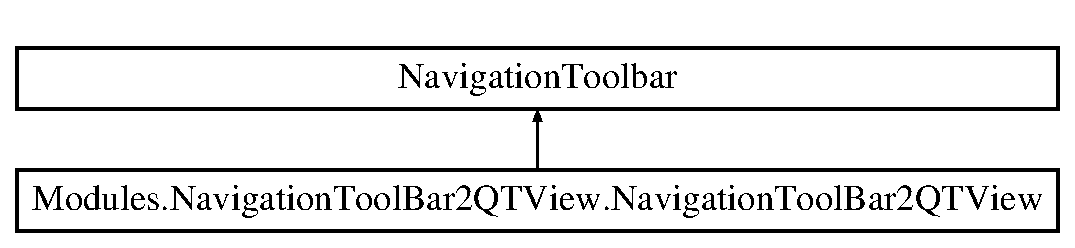
\includegraphics[height=2.000000cm]{classModules_1_1NavigationToolBar2QTView_1_1NavigationToolBar2QTView}
\end{center}
\end{figure}
\subsection*{Public Member Functions}
\begin{DoxyCompactItemize}
\item 
\hypertarget{classModules_1_1NavigationToolBar2QTView_1_1NavigationToolBar2QTView_a62770638b36d2748ca775dc8c9e60d8a}{def {\bfseries \-\_\-\-\_\-init\-\_\-\-\_\-}}\label{classModules_1_1NavigationToolBar2QTView_1_1NavigationToolBar2QTView_a62770638b36d2748ca775dc8c9e60d8a}

\end{DoxyCompactItemize}


The documentation for this class was generated from the following file\-:\begin{DoxyCompactItemize}
\item 
Modules/Navigation\-Tool\-Bar2\-Q\-T\-View.\-py\end{DoxyCompactItemize}

\hypertarget{classModules_1_1Null_1_1Null}{\section{Modules.\-Null.\-Null Class Reference}
\label{classModules_1_1Null_1_1Null}\index{Modules.\-Null.\-Null@{Modules.\-Null.\-Null}}
}
\subsection*{Public Member Functions}
\begin{DoxyCompactItemize}
\item 
\hypertarget{classModules_1_1Null_1_1Null_a7ff8cd6663d734a7582d4e588397244a}{def {\bfseries \-\_\-\-\_\-init\-\_\-\-\_\-}}\label{classModules_1_1Null_1_1Null_a7ff8cd6663d734a7582d4e588397244a}

\item 
\hypertarget{classModules_1_1Null_1_1Null_a8dd490d1b8537063dfb4da44e83d9c6b}{def {\bfseries \-\_\-\-\_\-call\-\_\-\-\_\-}}\label{classModules_1_1Null_1_1Null_a8dd490d1b8537063dfb4da44e83d9c6b}

\item 
\hypertarget{classModules_1_1Null_1_1Null_a4b43a6ade37c83bcb6caf3c97a5236a3}{def {\bfseries \-\_\-\-\_\-getattr\-\_\-\-\_\-}}\label{classModules_1_1Null_1_1Null_a4b43a6ade37c83bcb6caf3c97a5236a3}

\item 
\hypertarget{classModules_1_1Null_1_1Null_a577f0ba8a74805faca305691bd073a27}{def {\bfseries \-\_\-\-\_\-setattr\-\_\-\-\_\-}}\label{classModules_1_1Null_1_1Null_a577f0ba8a74805faca305691bd073a27}

\item 
\hypertarget{classModules_1_1Null_1_1Null_ad0e1184289fca7a72de66c52f25a30ca}{def {\bfseries \-\_\-\-\_\-delattr\-\_\-\-\_\-}}\label{classModules_1_1Null_1_1Null_ad0e1184289fca7a72de66c52f25a30ca}

\item 
\hypertarget{classModules_1_1Null_1_1Null_a05705a6e24061ba0713a446a7b82c513}{def {\bfseries \-\_\-\-\_\-repr\-\_\-\-\_\-}}\label{classModules_1_1Null_1_1Null_a05705a6e24061ba0713a446a7b82c513}

\item 
\hypertarget{classModules_1_1Null_1_1Null_ad8ab52973b61c6f93d80fec18bb81da9}{def {\bfseries \-\_\-\-\_\-str\-\_\-\-\_\-}}\label{classModules_1_1Null_1_1Null_ad8ab52973b61c6f93d80fec18bb81da9}

\end{DoxyCompactItemize}


\subsection{Detailed Description}
\begin{DoxyVerb}A class for implementing Null objects.

This class ignores all parameters passed when constructing or 
calling instances and traps all attribute and method requests. 
Instances of it always (and reliably) do 'nothing'.

The code might benefit from implementing some further special 
Python methods depending on the context in which its instances 
are used. Especially when comparing and coercing Null objects
the respective methods' implementation will depend very much
on the environment and, hence, these special methods are not
provided here.
\end{DoxyVerb}
 

The documentation for this class was generated from the following file\-:\begin{DoxyCompactItemize}
\item 
Modules/Null.\-py\end{DoxyCompactItemize}

\hypertarget{classpotku_1_1Potku}{\section{potku.\-Potku Class Reference}
\label{classpotku_1_1Potku}\index{potku.\-Potku@{potku.\-Potku}}
}
Inheritance diagram for potku.\-Potku\-:\begin{figure}[H]
\begin{center}
\leavevmode
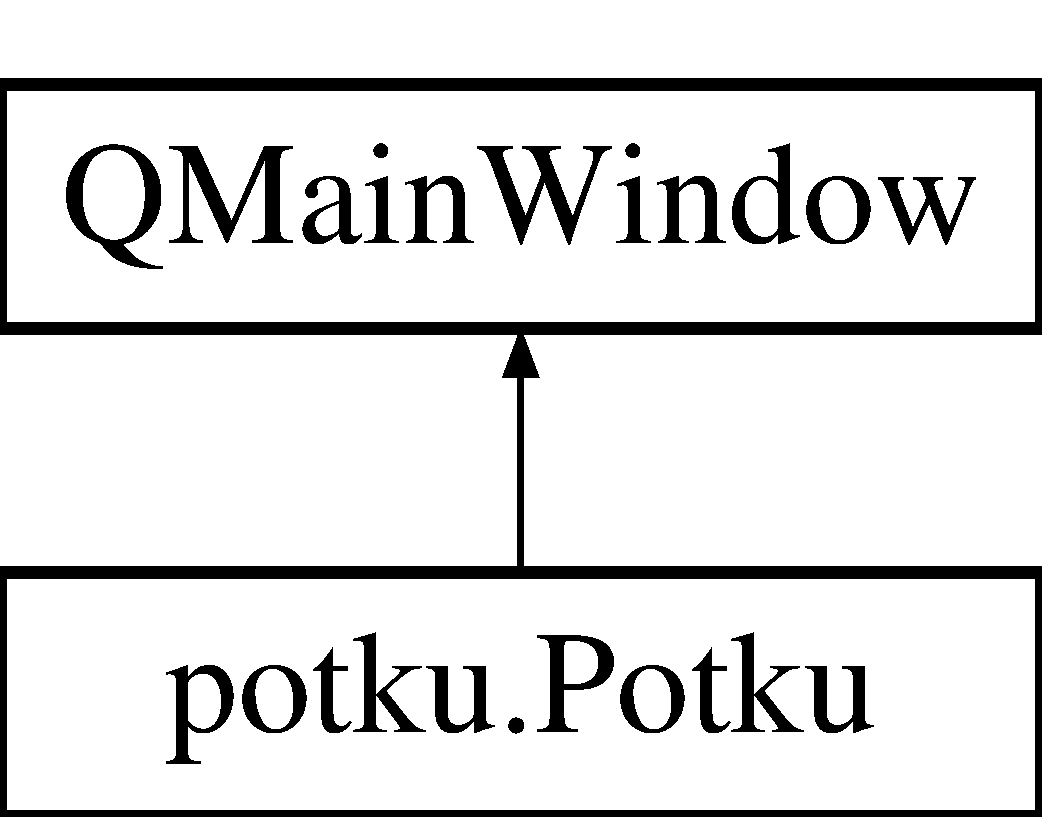
\includegraphics[height=2.000000cm]{classpotku_1_1Potku}
\end{center}
\end{figure}
\subsection*{Public Member Functions}
\begin{DoxyCompactItemize}
\item 
def \hyperlink{classpotku_1_1Potku_abacc6fcffce08f129e46912b46133980}{\-\_\-\-\_\-init\-\_\-\-\_\-}
\item 
def \hyperlink{classpotku_1_1Potku_ace8904ca1435e3ff39d022064d1b9e0e}{current\-\_\-measurement\-\_\-create\-\_\-depth\-\_\-profile}
\item 
def \hyperlink{classpotku_1_1Potku_a2e7801598b90f7fb0111765c7bc8d1da}{current\-\_\-measurement\-\_\-analyze\-\_\-elemental\-\_\-losses}
\item 
def \hyperlink{classpotku_1_1Potku_a11abb197b330cbc6d981536066b53cb9}{current\-\_\-measurement\-\_\-create\-\_\-energy\-\_\-spectrum}
\item 
def \hyperlink{classpotku_1_1Potku_a5b015e6566b0ec32ec03a519e498cbb3}{current\-\_\-measurement\-\_\-save\-\_\-cuts}
\item 
def \hyperlink{classpotku_1_1Potku_ae3ff955828ffc061f203028489060712}{delete\-\_\-selections}
\item 
def \hyperlink{classpotku_1_1Potku_a0b777a58cc571b39c9578574072c2ec8}{focus\-\_\-selected\-\_\-tab}
\item 
def \hyperlink{classpotku_1_1Potku_a7b6734d6454fe8f7e424a893f4adce6d}{hide\-\_\-panel}
\item 
def \hyperlink{classpotku_1_1Potku_a4bd36f54dc49a9da851a8fd04c3de6f5}{import\-\_\-pelletron}
\item 
def \hyperlink{classpotku_1_1Potku_a459c09c82e54c2fef28ca321ff1b0565}{import\-\_\-binary}
\item 
def \hyperlink{classpotku_1_1Potku_a6a563095f0717957f3009e228a55ddbe}{load\-\_\-project\-\_\-measurements}
\item 
def \hyperlink{classpotku_1_1Potku_a3c4fa17b8f0e571d2d5357ca7bc0ad67}{make\-\_\-new\-\_\-project}
\item 
def \hyperlink{classpotku_1_1Potku_ada5db2fbb788c3c13c997b6ea38b0048}{open\-\_\-about\-\_\-dialog}
\item 
def \hyperlink{classpotku_1_1Potku_a215b33676b4d5e5e561738b248002f88}{open\-\_\-global\-\_\-settings}
\item 
def \hyperlink{classpotku_1_1Potku_a27d976736e094d3921da22ffec8675d3}{open\-\_\-new\-\_\-measurement}
\item 
def \hyperlink{classpotku_1_1Potku_afe03b1f437b9085866226ee3a776be26}{open\-\_\-project}
\item 
def \hyperlink{classpotku_1_1Potku_ad3903c2c12be3d9f580f4113bdf7ff05}{open\-\_\-project\-\_\-settings}
\item 
def \hyperlink{classpotku_1_1Potku_a7156b065829863a689e6a11aafdd1d2f}{remove\-\_\-tab}
\end{DoxyCompactItemize}
\subsection*{Public Attributes}
\begin{DoxyCompactItemize}
\item 
\hypertarget{classpotku_1_1Potku_aca7058507a308f42cf48c31081957ec5}{{\bfseries ui}}\label{classpotku_1_1Potku_aca7058507a308f42cf48c31081957ec5}

\item 
\hypertarget{classpotku_1_1Potku_a792d75a421af67fc262b2ce9b73a5ac9}{{\bfseries title}}\label{classpotku_1_1Potku_a792d75a421af67fc262b2ce9b73a5ac9}

\item 
\hypertarget{classpotku_1_1Potku_a09b0f52e39fda656dc8b9af37192722e}{{\bfseries icon\-\_\-manager}}\label{classpotku_1_1Potku_a09b0f52e39fda656dc8b9af37192722e}

\item 
\hypertarget{classpotku_1_1Potku_a60425f7e1b40142bbefdd236369a8ddf}{{\bfseries settings}}\label{classpotku_1_1Potku_a60425f7e1b40142bbefdd236369a8ddf}

\item 
\hypertarget{classpotku_1_1Potku_a57c634eee881a8f40626072af58eb127}{{\bfseries project}}\label{classpotku_1_1Potku_a57c634eee881a8f40626072af58eb127}

\item 
\hypertarget{classpotku_1_1Potku_a2f1a58d78f83e6d687224903d2cfdf49}{{\bfseries masses}}\label{classpotku_1_1Potku_a2f1a58d78f83e6d687224903d2cfdf49}

\item 
\hypertarget{classpotku_1_1Potku_a910e6a13bcad092b7b3d032e201783da}{{\bfseries measurement\-\_\-tab\-\_\-widgets}}\label{classpotku_1_1Potku_a910e6a13bcad092b7b3d032e201783da}

\item 
\hypertarget{classpotku_1_1Potku_a41041603732ae1a8d9b9c28728c7541b}{{\bfseries tab\-\_\-id}}\label{classpotku_1_1Potku_a41041603732ae1a8d9b9c28728c7541b}

\item 
\hypertarget{classpotku_1_1Potku_a448ce351d466c6cd43a9462e14ca9f6a}{{\bfseries panel\-\_\-shown}}\label{classpotku_1_1Potku_a448ce351d466c6cd43a9462e14ca9f6a}

\end{DoxyCompactItemize}


\subsection{Detailed Description}
\begin{DoxyVerb}Potku is main window class.
\end{DoxyVerb}
 

\subsection{Constructor \& Destructor Documentation}
\hypertarget{classpotku_1_1Potku_abacc6fcffce08f129e46912b46133980}{\index{potku\-::\-Potku@{potku\-::\-Potku}!\-\_\-\-\_\-init\-\_\-\-\_\-@{\-\_\-\-\_\-init\-\_\-\-\_\-}}
\index{\-\_\-\-\_\-init\-\_\-\-\_\-@{\-\_\-\-\_\-init\-\_\-\-\_\-}!potku::Potku@{potku\-::\-Potku}}
\subsubsection[{\-\_\-\-\_\-init\-\_\-\-\_\-}]{\setlength{\rightskip}{0pt plus 5cm}def potku.\-Potku.\-\_\-\-\_\-init\-\_\-\-\_\- (
\begin{DoxyParamCaption}
\item[{}]{self}
\end{DoxyParamCaption}
)}}\label{classpotku_1_1Potku_abacc6fcffce08f129e46912b46133980}
\begin{DoxyVerb}Init main window for Potku.
\end{DoxyVerb}
 

\subsection{Member Function Documentation}
\hypertarget{classpotku_1_1Potku_a2e7801598b90f7fb0111765c7bc8d1da}{\index{potku\-::\-Potku@{potku\-::\-Potku}!current\-\_\-measurement\-\_\-analyze\-\_\-elemental\-\_\-losses@{current\-\_\-measurement\-\_\-analyze\-\_\-elemental\-\_\-losses}}
\index{current\-\_\-measurement\-\_\-analyze\-\_\-elemental\-\_\-losses@{current\-\_\-measurement\-\_\-analyze\-\_\-elemental\-\_\-losses}!potku::Potku@{potku\-::\-Potku}}
\subsubsection[{current\-\_\-measurement\-\_\-analyze\-\_\-elemental\-\_\-losses}]{\setlength{\rightskip}{0pt plus 5cm}def potku.\-Potku.\-current\-\_\-measurement\-\_\-analyze\-\_\-elemental\-\_\-losses (
\begin{DoxyParamCaption}
\item[{}]{self}
\end{DoxyParamCaption}
)}}\label{classpotku_1_1Potku_a2e7801598b90f7fb0111765c7bc8d1da}
\begin{DoxyVerb}Opens the element losses analyzation tool for the current open 
measurement tab widget.
\end{DoxyVerb}
 \hypertarget{classpotku_1_1Potku_ace8904ca1435e3ff39d022064d1b9e0e}{\index{potku\-::\-Potku@{potku\-::\-Potku}!current\-\_\-measurement\-\_\-create\-\_\-depth\-\_\-profile@{current\-\_\-measurement\-\_\-create\-\_\-depth\-\_\-profile}}
\index{current\-\_\-measurement\-\_\-create\-\_\-depth\-\_\-profile@{current\-\_\-measurement\-\_\-create\-\_\-depth\-\_\-profile}!potku::Potku@{potku\-::\-Potku}}
\subsubsection[{current\-\_\-measurement\-\_\-create\-\_\-depth\-\_\-profile}]{\setlength{\rightskip}{0pt plus 5cm}def potku.\-Potku.\-current\-\_\-measurement\-\_\-create\-\_\-depth\-\_\-profile (
\begin{DoxyParamCaption}
\item[{}]{self}
\end{DoxyParamCaption}
)}}\label{classpotku_1_1Potku_ace8904ca1435e3ff39d022064d1b9e0e}
\begin{DoxyVerb}Opens the depth profile analyzation tool for the current open 
measurement tab widget.
\end{DoxyVerb}
 \hypertarget{classpotku_1_1Potku_a11abb197b330cbc6d981536066b53cb9}{\index{potku\-::\-Potku@{potku\-::\-Potku}!current\-\_\-measurement\-\_\-create\-\_\-energy\-\_\-spectrum@{current\-\_\-measurement\-\_\-create\-\_\-energy\-\_\-spectrum}}
\index{current\-\_\-measurement\-\_\-create\-\_\-energy\-\_\-spectrum@{current\-\_\-measurement\-\_\-create\-\_\-energy\-\_\-spectrum}!potku::Potku@{potku\-::\-Potku}}
\subsubsection[{current\-\_\-measurement\-\_\-create\-\_\-energy\-\_\-spectrum}]{\setlength{\rightskip}{0pt plus 5cm}def potku.\-Potku.\-current\-\_\-measurement\-\_\-create\-\_\-energy\-\_\-spectrum (
\begin{DoxyParamCaption}
\item[{}]{self}
\end{DoxyParamCaption}
)}}\label{classpotku_1_1Potku_a11abb197b330cbc6d981536066b53cb9}
\begin{DoxyVerb}Opens the energy spectrum analyzation tool for the current open 
measurement tab widget.
\end{DoxyVerb}
 \hypertarget{classpotku_1_1Potku_a5b015e6566b0ec32ec03a519e498cbb3}{\index{potku\-::\-Potku@{potku\-::\-Potku}!current\-\_\-measurement\-\_\-save\-\_\-cuts@{current\-\_\-measurement\-\_\-save\-\_\-cuts}}
\index{current\-\_\-measurement\-\_\-save\-\_\-cuts@{current\-\_\-measurement\-\_\-save\-\_\-cuts}!potku::Potku@{potku\-::\-Potku}}
\subsubsection[{current\-\_\-measurement\-\_\-save\-\_\-cuts}]{\setlength{\rightskip}{0pt plus 5cm}def potku.\-Potku.\-current\-\_\-measurement\-\_\-save\-\_\-cuts (
\begin{DoxyParamCaption}
\item[{}]{self}
\end{DoxyParamCaption}
)}}\label{classpotku_1_1Potku_a5b015e6566b0ec32ec03a519e498cbb3}
\begin{DoxyVerb}Saves the current open measurement tab widget's selected cuts 
to cut files.
\end{DoxyVerb}
 \hypertarget{classpotku_1_1Potku_ae3ff955828ffc061f203028489060712}{\index{potku\-::\-Potku@{potku\-::\-Potku}!delete\-\_\-selections@{delete\-\_\-selections}}
\index{delete\-\_\-selections@{delete\-\_\-selections}!potku::Potku@{potku\-::\-Potku}}
\subsubsection[{delete\-\_\-selections}]{\setlength{\rightskip}{0pt plus 5cm}def potku.\-Potku.\-delete\-\_\-selections (
\begin{DoxyParamCaption}
\item[{}]{self}
\end{DoxyParamCaption}
)}}\label{classpotku_1_1Potku_ae3ff955828ffc061f203028489060712}
\begin{DoxyVerb}Deletes the selected tree widget items.
\end{DoxyVerb}
 \hypertarget{classpotku_1_1Potku_a0b777a58cc571b39c9578574072c2ec8}{\index{potku\-::\-Potku@{potku\-::\-Potku}!focus\-\_\-selected\-\_\-tab@{focus\-\_\-selected\-\_\-tab}}
\index{focus\-\_\-selected\-\_\-tab@{focus\-\_\-selected\-\_\-tab}!potku::Potku@{potku\-::\-Potku}}
\subsubsection[{focus\-\_\-selected\-\_\-tab}]{\setlength{\rightskip}{0pt plus 5cm}def potku.\-Potku.\-focus\-\_\-selected\-\_\-tab (
\begin{DoxyParamCaption}
\item[{}]{self, }
\item[{}]{clicked\-\_\-item}
\end{DoxyParamCaption}
)}}\label{classpotku_1_1Potku_a0b777a58cc571b39c9578574072c2ec8}
\begin{DoxyVerb}Focus to selected tab (in tree widget) and if it isn't open, open it.

Args:
    clicked_item: TreeWidgetItem with tab_id attribute (int) that connects
    the item to the corresponding MeasurementTabWidget
\end{DoxyVerb}
 \hypertarget{classpotku_1_1Potku_a7b6734d6454fe8f7e424a893f4adce6d}{\index{potku\-::\-Potku@{potku\-::\-Potku}!hide\-\_\-panel@{hide\-\_\-panel}}
\index{hide\-\_\-panel@{hide\-\_\-panel}!potku::Potku@{potku\-::\-Potku}}
\subsubsection[{hide\-\_\-panel}]{\setlength{\rightskip}{0pt plus 5cm}def potku.\-Potku.\-hide\-\_\-panel (
\begin{DoxyParamCaption}
\item[{}]{self, }
\item[{}]{enable\-\_\-hide = {\ttfamily None}}
\end{DoxyParamCaption}
)}}\label{classpotku_1_1Potku_a7b6734d6454fe8f7e424a893f4adce6d}
\begin{DoxyVerb}Sets the frame (including measurement navigation view, global 
settings and project settings buttons) visible.

Args:
    enable_hide: If True, sets the frame visible and vice versa. 
    If not given, sets the frame visible or hidden depending its 
    previous state.
\end{DoxyVerb}
 \hypertarget{classpotku_1_1Potku_a459c09c82e54c2fef28ca321ff1b0565}{\index{potku\-::\-Potku@{potku\-::\-Potku}!import\-\_\-binary@{import\-\_\-binary}}
\index{import\-\_\-binary@{import\-\_\-binary}!potku::Potku@{potku\-::\-Potku}}
\subsubsection[{import\-\_\-binary}]{\setlength{\rightskip}{0pt plus 5cm}def potku.\-Potku.\-import\-\_\-binary (
\begin{DoxyParamCaption}
\item[{}]{self}
\end{DoxyParamCaption}
)}}\label{classpotku_1_1Potku_a459c09c82e54c2fef28ca321ff1b0565}
\begin{DoxyVerb}Import binary measurements into project.

Import binary measurements from 
\end{DoxyVerb}
 \hypertarget{classpotku_1_1Potku_a4bd36f54dc49a9da851a8fd04c3de6f5}{\index{potku\-::\-Potku@{potku\-::\-Potku}!import\-\_\-pelletron@{import\-\_\-pelletron}}
\index{import\-\_\-pelletron@{import\-\_\-pelletron}!potku::Potku@{potku\-::\-Potku}}
\subsubsection[{import\-\_\-pelletron}]{\setlength{\rightskip}{0pt plus 5cm}def potku.\-Potku.\-import\-\_\-pelletron (
\begin{DoxyParamCaption}
\item[{}]{self}
\end{DoxyParamCaption}
)}}\label{classpotku_1_1Potku_a4bd36f54dc49a9da851a8fd04c3de6f5}
\begin{DoxyVerb}Import Pelletron's measurements into project.

Import Pelletron's measurements from 
\end{DoxyVerb}
 \hypertarget{classpotku_1_1Potku_a6a563095f0717957f3009e228a55ddbe}{\index{potku\-::\-Potku@{potku\-::\-Potku}!load\-\_\-project\-\_\-measurements@{load\-\_\-project\-\_\-measurements}}
\index{load\-\_\-project\-\_\-measurements@{load\-\_\-project\-\_\-measurements}!potku::Potku@{potku\-::\-Potku}}
\subsubsection[{load\-\_\-project\-\_\-measurements}]{\setlength{\rightskip}{0pt plus 5cm}def potku.\-Potku.\-load\-\_\-project\-\_\-measurements (
\begin{DoxyParamCaption}
\item[{}]{self, }
\item[{}]{measurements = {\ttfamily \mbox{[}\mbox{]}}}
\end{DoxyParamCaption}
)}}\label{classpotku_1_1Potku_a6a563095f0717957f3009e228a55ddbe}
\begin{DoxyVerb}Load measurement files in the project.

Args:
    measurements: A list representing loadable measurements when importing
          measurements to the project.
\end{DoxyVerb}
 \hypertarget{classpotku_1_1Potku_a3c4fa17b8f0e571d2d5357ca7bc0ad67}{\index{potku\-::\-Potku@{potku\-::\-Potku}!make\-\_\-new\-\_\-project@{make\-\_\-new\-\_\-project}}
\index{make\-\_\-new\-\_\-project@{make\-\_\-new\-\_\-project}!potku::Potku@{potku\-::\-Potku}}
\subsubsection[{make\-\_\-new\-\_\-project}]{\setlength{\rightskip}{0pt plus 5cm}def potku.\-Potku.\-make\-\_\-new\-\_\-project (
\begin{DoxyParamCaption}
\item[{}]{self}
\end{DoxyParamCaption}
)}}\label{classpotku_1_1Potku_a3c4fa17b8f0e571d2d5357ca7bc0ad67}
\begin{DoxyVerb}Opens a dialog for creating a new project.
\end{DoxyVerb}
 \hypertarget{classpotku_1_1Potku_ada5db2fbb788c3c13c997b6ea38b0048}{\index{potku\-::\-Potku@{potku\-::\-Potku}!open\-\_\-about\-\_\-dialog@{open\-\_\-about\-\_\-dialog}}
\index{open\-\_\-about\-\_\-dialog@{open\-\_\-about\-\_\-dialog}!potku::Potku@{potku\-::\-Potku}}
\subsubsection[{open\-\_\-about\-\_\-dialog}]{\setlength{\rightskip}{0pt plus 5cm}def potku.\-Potku.\-open\-\_\-about\-\_\-dialog (
\begin{DoxyParamCaption}
\item[{}]{self}
\end{DoxyParamCaption}
)}}\label{classpotku_1_1Potku_ada5db2fbb788c3c13c997b6ea38b0048}
\begin{DoxyVerb}Show Potku program about dialog.
\end{DoxyVerb}
 \hypertarget{classpotku_1_1Potku_a215b33676b4d5e5e561738b248002f88}{\index{potku\-::\-Potku@{potku\-::\-Potku}!open\-\_\-global\-\_\-settings@{open\-\_\-global\-\_\-settings}}
\index{open\-\_\-global\-\_\-settings@{open\-\_\-global\-\_\-settings}!potku::Potku@{potku\-::\-Potku}}
\subsubsection[{open\-\_\-global\-\_\-settings}]{\setlength{\rightskip}{0pt plus 5cm}def potku.\-Potku.\-open\-\_\-global\-\_\-settings (
\begin{DoxyParamCaption}
\item[{}]{self}
\end{DoxyParamCaption}
)}}\label{classpotku_1_1Potku_a215b33676b4d5e5e561738b248002f88}
\begin{DoxyVerb}Opens global settings dialog.
\end{DoxyVerb}
 \hypertarget{classpotku_1_1Potku_a27d976736e094d3921da22ffec8675d3}{\index{potku\-::\-Potku@{potku\-::\-Potku}!open\-\_\-new\-\_\-measurement@{open\-\_\-new\-\_\-measurement}}
\index{open\-\_\-new\-\_\-measurement@{open\-\_\-new\-\_\-measurement}!potku::Potku@{potku\-::\-Potku}}
\subsubsection[{open\-\_\-new\-\_\-measurement}]{\setlength{\rightskip}{0pt plus 5cm}def potku.\-Potku.\-open\-\_\-new\-\_\-measurement (
\begin{DoxyParamCaption}
\item[{}]{self}
\end{DoxyParamCaption}
)}}\label{classpotku_1_1Potku_a27d976736e094d3921da22ffec8675d3}
\begin{DoxyVerb}Opens file an open dialog and if filename is given opens new measurement 
from it.
\end{DoxyVerb}
 \hypertarget{classpotku_1_1Potku_afe03b1f437b9085866226ee3a776be26}{\index{potku\-::\-Potku@{potku\-::\-Potku}!open\-\_\-project@{open\-\_\-project}}
\index{open\-\_\-project@{open\-\_\-project}!potku::Potku@{potku\-::\-Potku}}
\subsubsection[{open\-\_\-project}]{\setlength{\rightskip}{0pt plus 5cm}def potku.\-Potku.\-open\-\_\-project (
\begin{DoxyParamCaption}
\item[{}]{self}
\end{DoxyParamCaption}
)}}\label{classpotku_1_1Potku_afe03b1f437b9085866226ee3a776be26}
\begin{DoxyVerb}Shows a dialog to open a project.
\end{DoxyVerb}
 \hypertarget{classpotku_1_1Potku_ad3903c2c12be3d9f580f4113bdf7ff05}{\index{potku\-::\-Potku@{potku\-::\-Potku}!open\-\_\-project\-\_\-settings@{open\-\_\-project\-\_\-settings}}
\index{open\-\_\-project\-\_\-settings@{open\-\_\-project\-\_\-settings}!potku::Potku@{potku\-::\-Potku}}
\subsubsection[{open\-\_\-project\-\_\-settings}]{\setlength{\rightskip}{0pt plus 5cm}def potku.\-Potku.\-open\-\_\-project\-\_\-settings (
\begin{DoxyParamCaption}
\item[{}]{self}
\end{DoxyParamCaption}
)}}\label{classpotku_1_1Potku_ad3903c2c12be3d9f580f4113bdf7ff05}
\begin{DoxyVerb}Opens project settings dialog.
\end{DoxyVerb}
 \hypertarget{classpotku_1_1Potku_a7156b065829863a689e6a11aafdd1d2f}{\index{potku\-::\-Potku@{potku\-::\-Potku}!remove\-\_\-tab@{remove\-\_\-tab}}
\index{remove\-\_\-tab@{remove\-\_\-tab}!potku::Potku@{potku\-::\-Potku}}
\subsubsection[{remove\-\_\-tab}]{\setlength{\rightskip}{0pt plus 5cm}def potku.\-Potku.\-remove\-\_\-tab (
\begin{DoxyParamCaption}
\item[{}]{self, }
\item[{}]{tab\-\_\-index}
\end{DoxyParamCaption}
)}}\label{classpotku_1_1Potku_a7156b065829863a689e6a11aafdd1d2f}
\begin{DoxyVerb}Remove tab which's close button has been pressed.

Args:
    tab_index: Integer representing index of the current tab
\end{DoxyVerb}
 

The documentation for this class was generated from the following file\-:\begin{DoxyCompactItemize}
\item 
potku.\-py\end{DoxyCompactItemize}

\hypertarget{classModules_1_1Project_1_1Project}{\section{Modules.\-Project.\-Project Class Reference}
\label{classModules_1_1Project_1_1Project}\index{Modules.\-Project.\-Project@{Modules.\-Project.\-Project}}
}
\subsection*{Public Member Functions}
\begin{DoxyCompactItemize}
\item 
def \hyperlink{classModules_1_1Project_1_1Project_a8b518c632e7abf15987810130671bd41}{\-\_\-\-\_\-init\-\_\-\-\_\-}
\item 
def \hyperlink{classModules_1_1Project_1_1Project_a51c72dd6e4387f92f5e41cef8b7d56db}{exclude\-\_\-slave}
\item 
def \hyperlink{classModules_1_1Project_1_1Project_ac660b915cc6bdff73d3eeae889f16918}{include\-\_\-slave}
\item 
def \hyperlink{classModules_1_1Project_1_1Project_a3db947d315829ee0e06b05be01aa8544}{get\-\_\-name}
\item 
def \hyperlink{classModules_1_1Project_1_1Project_a234229c766c554aa3c3a51b9f3a77ec8}{get\-\_\-master}
\item 
def \hyperlink{classModules_1_1Project_1_1Project_a598802299ac415e65888ab70140e89bc}{get\-\_\-measurements\-\_\-files}
\item 
def \hyperlink{classModules_1_1Project_1_1Project_a00a02f9db1709eef854920f0b579e6c0}{get\-\_\-measurement\-\_\-tabs}
\item 
def \hyperlink{classModules_1_1Project_1_1Project_a51a80de6a442b545c5cd60d840656460}{get\-\_\-nonslaves}
\item 
def \hyperlink{classModules_1_1Project_1_1Project_a86c216b2840c36076ad715914a5e43b8}{has\-\_\-master}
\item 
def \hyperlink{classModules_1_1Project_1_1Project_ab0b85dc510ae06fce07c18e9612343ab}{load}
\item 
def \hyperlink{classModules_1_1Project_1_1Project_a31663ab8365b326f3645049c20e79584}{save}
\item 
def \hyperlink{classModules_1_1Project_1_1Project_a3370b1b3818eb2fb3d1b1e14d3ea7cc2}{save\-\_\-cuts}
\item 
def \hyperlink{classModules_1_1Project_1_1Project_a66db9bc0dd3fc8c691a673150e6cff5a}{save\-\_\-selection}
\item 
def \hyperlink{classModules_1_1Project_1_1Project_a3c3ae9458c4ccea13f75935d57ce6d99}{set\-\_\-master}
\end{DoxyCompactItemize}
\subsection*{Public Attributes}
\begin{DoxyCompactItemize}
\item 
\hypertarget{classModules_1_1Project_1_1Project_a4ca9a39c52317a99cb5a63ee8fe2d7be}{{\bfseries directory}}\label{classModules_1_1Project_1_1Project_a4ca9a39c52317a99cb5a63ee8fe2d7be}

\item 
\hypertarget{classModules_1_1Project_1_1Project_acd6ef32f39ac825efa91ad2c50c63117}{{\bfseries project\-\_\-name}}\label{classModules_1_1Project_1_1Project_acd6ef32f39ac825efa91ad2c50c63117}

\item 
\hypertarget{classModules_1_1Project_1_1Project_a66db98ab8316f1b35cb5df58b9dd4cca}{{\bfseries settings}}\label{classModules_1_1Project_1_1Project_a66db98ab8316f1b35cb5df58b9dd4cca}

\item 
\hypertarget{classModules_1_1Project_1_1Project_ac29d11dae4aea275cc6247aecf03eb4e}{{\bfseries global\-\_\-settings}}\label{classModules_1_1Project_1_1Project_ac29d11dae4aea275cc6247aecf03eb4e}

\item 
\hypertarget{classModules_1_1Project_1_1Project_a189dd217f3436b3eec212260786c085b}{{\bfseries masses}}\label{classModules_1_1Project_1_1Project_a189dd217f3436b3eec212260786c085b}

\item 
\hypertarget{classModules_1_1Project_1_1Project_a60c03a0d1e7fe102b926877b8e7914b0}{{\bfseries statusbar}}\label{classModules_1_1Project_1_1Project_a60c03a0d1e7fe102b926877b8e7914b0}

\item 
\hypertarget{classModules_1_1Project_1_1Project_af98cc5dca4e342077fc44f212590360e}{{\bfseries measurements}}\label{classModules_1_1Project_1_1Project_af98cc5dca4e342077fc44f212590360e}

\item 
\hypertarget{classModules_1_1Project_1_1Project_a54961ce1e0e42740a3c7e81154cd75b4}{{\bfseries project\-\_\-file}}\label{classModules_1_1Project_1_1Project_a54961ce1e0e42740a3c7e81154cd75b4}

\end{DoxyCompactItemize}


\subsection{Detailed Description}
\begin{DoxyVerb}Project class to handle all measurements.
\end{DoxyVerb}
 

\subsection{Constructor \& Destructor Documentation}
\hypertarget{classModules_1_1Project_1_1Project_a8b518c632e7abf15987810130671bd41}{\index{Modules\-::\-Project\-::\-Project@{Modules\-::\-Project\-::\-Project}!\-\_\-\-\_\-init\-\_\-\-\_\-@{\-\_\-\-\_\-init\-\_\-\-\_\-}}
\index{\-\_\-\-\_\-init\-\_\-\-\_\-@{\-\_\-\-\_\-init\-\_\-\-\_\-}!Modules::Project::Project@{Modules\-::\-Project\-::\-Project}}
\subsubsection[{\-\_\-\-\_\-init\-\_\-\-\_\-}]{\setlength{\rightskip}{0pt plus 5cm}def Modules.\-Project.\-Project.\-\_\-\-\_\-init\-\_\-\-\_\- (
\begin{DoxyParamCaption}
\item[{}]{self, }
\item[{}]{directory, }
\item[{}]{name, }
\item[{}]{masses, }
\item[{}]{statusbar, }
\item[{}]{global\-\_\-settings, }
\item[{}]{measurement\-\_\-tabs}
\end{DoxyParamCaption}
)}}\label{classModules_1_1Project_1_1Project_a8b518c632e7abf15987810130671bd41}
\begin{DoxyVerb}Inits Project class. 

Args:
    directory: A String representing project directory.
    masses: A Masses class object.
    statusbar: A QtGui.QMainWindow's QStatusBar.
    global_settings: A GlobalSettings class object (of the program).
    measurement_tabs: A dictionary of MeasurementTabWidgets of the 
              measurements in the project.
\end{DoxyVerb}
 

\subsection{Member Function Documentation}
\hypertarget{classModules_1_1Project_1_1Project_a51c72dd6e4387f92f5e41cef8b7d56db}{\index{Modules\-::\-Project\-::\-Project@{Modules\-::\-Project\-::\-Project}!exclude\-\_\-slave@{exclude\-\_\-slave}}
\index{exclude\-\_\-slave@{exclude\-\_\-slave}!Modules::Project::Project@{Modules\-::\-Project\-::\-Project}}
\subsubsection[{exclude\-\_\-slave}]{\setlength{\rightskip}{0pt plus 5cm}def Modules.\-Project.\-Project.\-exclude\-\_\-slave (
\begin{DoxyParamCaption}
\item[{}]{self, }
\item[{}]{measurement}
\end{DoxyParamCaption}
)}}\label{classModules_1_1Project_1_1Project_a51c72dd6e4387f92f5e41cef8b7d56db}
\begin{DoxyVerb}Exclude measurement from slave category under master.

Args:
    measurement: A measurement class object.
\end{DoxyVerb}
 \hypertarget{classModules_1_1Project_1_1Project_a234229c766c554aa3c3a51b9f3a77ec8}{\index{Modules\-::\-Project\-::\-Project@{Modules\-::\-Project\-::\-Project}!get\-\_\-master@{get\-\_\-master}}
\index{get\-\_\-master@{get\-\_\-master}!Modules::Project::Project@{Modules\-::\-Project\-::\-Project}}
\subsubsection[{get\-\_\-master}]{\setlength{\rightskip}{0pt plus 5cm}def Modules.\-Project.\-Project.\-get\-\_\-master (
\begin{DoxyParamCaption}
\item[{}]{self}
\end{DoxyParamCaption}
)}}\label{classModules_1_1Project_1_1Project_a234229c766c554aa3c3a51b9f3a77ec8}
\begin{DoxyVerb}Get master measurement of the project.
\end{DoxyVerb}
 \hypertarget{classModules_1_1Project_1_1Project_a00a02f9db1709eef854920f0b579e6c0}{\index{Modules\-::\-Project\-::\-Project@{Modules\-::\-Project\-::\-Project}!get\-\_\-measurement\-\_\-tabs@{get\-\_\-measurement\-\_\-tabs}}
\index{get\-\_\-measurement\-\_\-tabs@{get\-\_\-measurement\-\_\-tabs}!Modules::Project::Project@{Modules\-::\-Project\-::\-Project}}
\subsubsection[{get\-\_\-measurement\-\_\-tabs}]{\setlength{\rightskip}{0pt plus 5cm}def Modules.\-Project.\-Project.\-get\-\_\-measurement\-\_\-tabs (
\begin{DoxyParamCaption}
\item[{}]{self, }
\item[{}]{exclude\-\_\-id = {\ttfamily -\/1}}
\end{DoxyParamCaption}
)}}\label{classModules_1_1Project_1_1Project_a00a02f9db1709eef854920f0b579e6c0}
\begin{DoxyVerb}Get measurement tabs of a project.
\end{DoxyVerb}
 \hypertarget{classModules_1_1Project_1_1Project_a598802299ac415e65888ab70140e89bc}{\index{Modules\-::\-Project\-::\-Project@{Modules\-::\-Project\-::\-Project}!get\-\_\-measurements\-\_\-files@{get\-\_\-measurements\-\_\-files}}
\index{get\-\_\-measurements\-\_\-files@{get\-\_\-measurements\-\_\-files}!Modules::Project::Project@{Modules\-::\-Project\-::\-Project}}
\subsubsection[{get\-\_\-measurements\-\_\-files}]{\setlength{\rightskip}{0pt plus 5cm}def Modules.\-Project.\-Project.\-get\-\_\-measurements\-\_\-files (
\begin{DoxyParamCaption}
\item[{}]{self}
\end{DoxyParamCaption}
)}}\label{classModules_1_1Project_1_1Project_a598802299ac415e65888ab70140e89bc}
\begin{DoxyVerb}Get measurements files inside project folder.
\end{DoxyVerb}
 \hypertarget{classModules_1_1Project_1_1Project_a3db947d315829ee0e06b05be01aa8544}{\index{Modules\-::\-Project\-::\-Project@{Modules\-::\-Project\-::\-Project}!get\-\_\-name@{get\-\_\-name}}
\index{get\-\_\-name@{get\-\_\-name}!Modules::Project::Project@{Modules\-::\-Project\-::\-Project}}
\subsubsection[{get\-\_\-name}]{\setlength{\rightskip}{0pt plus 5cm}def Modules.\-Project.\-Project.\-get\-\_\-name (
\begin{DoxyParamCaption}
\item[{}]{self}
\end{DoxyParamCaption}
)}}\label{classModules_1_1Project_1_1Project_a3db947d315829ee0e06b05be01aa8544}
\begin{DoxyVerb}Get the project's name.

Return:
    Returns the project's name.
\end{DoxyVerb}
 \hypertarget{classModules_1_1Project_1_1Project_a51a80de6a442b545c5cd60d840656460}{\index{Modules\-::\-Project\-::\-Project@{Modules\-::\-Project\-::\-Project}!get\-\_\-nonslaves@{get\-\_\-nonslaves}}
\index{get\-\_\-nonslaves@{get\-\_\-nonslaves}!Modules::Project::Project@{Modules\-::\-Project\-::\-Project}}
\subsubsection[{get\-\_\-nonslaves}]{\setlength{\rightskip}{0pt plus 5cm}def Modules.\-Project.\-Project.\-get\-\_\-nonslaves (
\begin{DoxyParamCaption}
\item[{}]{self}
\end{DoxyParamCaption}
)}}\label{classModules_1_1Project_1_1Project_a51a80de6a442b545c5cd60d840656460}
\begin{DoxyVerb}Get measurement names that will be excluded from slave category.
\end{DoxyVerb}
 \hypertarget{classModules_1_1Project_1_1Project_a86c216b2840c36076ad715914a5e43b8}{\index{Modules\-::\-Project\-::\-Project@{Modules\-::\-Project\-::\-Project}!has\-\_\-master@{has\-\_\-master}}
\index{has\-\_\-master@{has\-\_\-master}!Modules::Project::Project@{Modules\-::\-Project\-::\-Project}}
\subsubsection[{has\-\_\-master}]{\setlength{\rightskip}{0pt plus 5cm}def Modules.\-Project.\-Project.\-has\-\_\-master (
\begin{DoxyParamCaption}
\item[{}]{self}
\end{DoxyParamCaption}
)}}\label{classModules_1_1Project_1_1Project_a86c216b2840c36076ad715914a5e43b8}
\begin{DoxyVerb}Does project have master measurement? Check from config file as
it is not loaded yet.

This is used when loading project. As project has no measurement in it
when inited so check is made in potku.py after loading all measurements
via this method. The corresponding master title in treewidget is then set.
\end{DoxyVerb}
 \hypertarget{classModules_1_1Project_1_1Project_ac660b915cc6bdff73d3eeae889f16918}{\index{Modules\-::\-Project\-::\-Project@{Modules\-::\-Project\-::\-Project}!include\-\_\-slave@{include\-\_\-slave}}
\index{include\-\_\-slave@{include\-\_\-slave}!Modules::Project::Project@{Modules\-::\-Project\-::\-Project}}
\subsubsection[{include\-\_\-slave}]{\setlength{\rightskip}{0pt plus 5cm}def Modules.\-Project.\-Project.\-include\-\_\-slave (
\begin{DoxyParamCaption}
\item[{}]{self, }
\item[{}]{measurement}
\end{DoxyParamCaption}
)}}\label{classModules_1_1Project_1_1Project_ac660b915cc6bdff73d3eeae889f16918}
\begin{DoxyVerb}Include measurement to slave category under master.

Args:
    measurement: A measurement class object.
\end{DoxyVerb}
 \hypertarget{classModules_1_1Project_1_1Project_ab0b85dc510ae06fce07c18e9612343ab}{\index{Modules\-::\-Project\-::\-Project@{Modules\-::\-Project\-::\-Project}!load@{load}}
\index{load@{load}!Modules::Project::Project@{Modules\-::\-Project\-::\-Project}}
\subsubsection[{load}]{\setlength{\rightskip}{0pt plus 5cm}def Modules.\-Project.\-Project.\-load (
\begin{DoxyParamCaption}
\item[{}]{self}
\end{DoxyParamCaption}
)}}\label{classModules_1_1Project_1_1Project_ab0b85dc510ae06fce07c18e9612343ab}
\begin{DoxyVerb}Load project
\end{DoxyVerb}
 \hypertarget{classModules_1_1Project_1_1Project_a31663ab8365b326f3645049c20e79584}{\index{Modules\-::\-Project\-::\-Project@{Modules\-::\-Project\-::\-Project}!save@{save}}
\index{save@{save}!Modules::Project::Project@{Modules\-::\-Project\-::\-Project}}
\subsubsection[{save}]{\setlength{\rightskip}{0pt plus 5cm}def Modules.\-Project.\-Project.\-save (
\begin{DoxyParamCaption}
\item[{}]{self}
\end{DoxyParamCaption}
)}}\label{classModules_1_1Project_1_1Project_a31663ab8365b326f3645049c20e79584}
\begin{DoxyVerb}Save project
\end{DoxyVerb}
 \hypertarget{classModules_1_1Project_1_1Project_a3370b1b3818eb2fb3d1b1e14d3ea7cc2}{\index{Modules\-::\-Project\-::\-Project@{Modules\-::\-Project\-::\-Project}!save\-\_\-cuts@{save\-\_\-cuts}}
\index{save\-\_\-cuts@{save\-\_\-cuts}!Modules::Project::Project@{Modules\-::\-Project\-::\-Project}}
\subsubsection[{save\-\_\-cuts}]{\setlength{\rightskip}{0pt plus 5cm}def Modules.\-Project.\-Project.\-save\-\_\-cuts (
\begin{DoxyParamCaption}
\item[{}]{self, }
\item[{}]{measurement}
\end{DoxyParamCaption}
)}}\label{classModules_1_1Project_1_1Project_a3370b1b3818eb2fb3d1b1e14d3ea7cc2}
\begin{DoxyVerb}Save cuts for all measurements except for master.

Args:
    measurement: A measurement class object that issued save cuts.
\end{DoxyVerb}
 \hypertarget{classModules_1_1Project_1_1Project_a66db9bc0dd3fc8c691a673150e6cff5a}{\index{Modules\-::\-Project\-::\-Project@{Modules\-::\-Project\-::\-Project}!save\-\_\-selection@{save\-\_\-selection}}
\index{save\-\_\-selection@{save\-\_\-selection}!Modules::Project::Project@{Modules\-::\-Project\-::\-Project}}
\subsubsection[{save\-\_\-selection}]{\setlength{\rightskip}{0pt plus 5cm}def Modules.\-Project.\-Project.\-save\-\_\-selection (
\begin{DoxyParamCaption}
\item[{}]{self, }
\item[{}]{measurement}
\end{DoxyParamCaption}
)}}\label{classModules_1_1Project_1_1Project_a66db9bc0dd3fc8c691a673150e6cff5a}
\begin{DoxyVerb}Save selection for all measurements except for master.

Args:
    measurement: A measurement class object that issued save cuts.
\end{DoxyVerb}
 \hypertarget{classModules_1_1Project_1_1Project_a3c3ae9458c4ccea13f75935d57ce6d99}{\index{Modules\-::\-Project\-::\-Project@{Modules\-::\-Project\-::\-Project}!set\-\_\-master@{set\-\_\-master}}
\index{set\-\_\-master@{set\-\_\-master}!Modules::Project::Project@{Modules\-::\-Project\-::\-Project}}
\subsubsection[{set\-\_\-master}]{\setlength{\rightskip}{0pt plus 5cm}def Modules.\-Project.\-Project.\-set\-\_\-master (
\begin{DoxyParamCaption}
\item[{}]{self, }
\item[{}]{measurement = {\ttfamily None}}
\end{DoxyParamCaption}
)}}\label{classModules_1_1Project_1_1Project_a3c3ae9458c4ccea13f75935d57ce6d99}
\begin{DoxyVerb}Set master measurement for the project.

Args:
    measurement: A measurement class object.
\end{DoxyVerb}
 

The documentation for this class was generated from the following file\-:\begin{DoxyCompactItemize}
\item 
Modules/Project.\-py\end{DoxyCompactItemize}

\hypertarget{classDialogs_1_1ProjectNewDialog_1_1ProjectNewDialog}{\section{Dialogs.\-Project\-New\-Dialog.\-Project\-New\-Dialog Class Reference}
\label{classDialogs_1_1ProjectNewDialog_1_1ProjectNewDialog}\index{Dialogs.\-Project\-New\-Dialog.\-Project\-New\-Dialog@{Dialogs.\-Project\-New\-Dialog.\-Project\-New\-Dialog}}
}
Inheritance diagram for Dialogs.\-Project\-New\-Dialog.\-Project\-New\-Dialog\-:\begin{figure}[H]
\begin{center}
\leavevmode
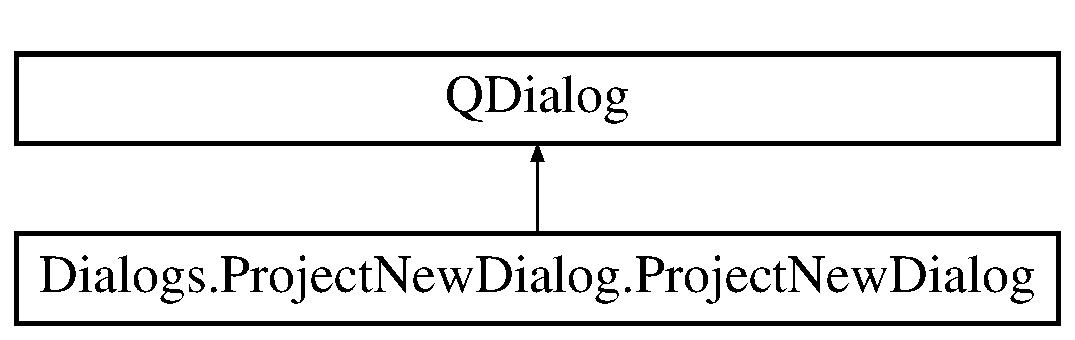
\includegraphics[height=2.000000cm]{classDialogs_1_1ProjectNewDialog_1_1ProjectNewDialog}
\end{center}
\end{figure}
\subsection*{Public Member Functions}
\begin{DoxyCompactItemize}
\item 
def \hyperlink{classDialogs_1_1ProjectNewDialog_1_1ProjectNewDialog_ae02082b6c5cf4bf0a80a138360467787}{\-\_\-\-\_\-init\-\_\-\-\_\-}
\end{DoxyCompactItemize}
\subsection*{Public Attributes}
\begin{DoxyCompactItemize}
\item 
\hypertarget{classDialogs_1_1ProjectNewDialog_1_1ProjectNewDialog_ab5d089642593b76fe49fef6fbe1a96e8}{{\bfseries parent}}\label{classDialogs_1_1ProjectNewDialog_1_1ProjectNewDialog_ab5d089642593b76fe49fef6fbe1a96e8}

\item 
\hypertarget{classDialogs_1_1ProjectNewDialog_1_1ProjectNewDialog_a85e90c94e8e65d47bfea464e80b5ab95}{{\bfseries folder}}\label{classDialogs_1_1ProjectNewDialog_1_1ProjectNewDialog_a85e90c94e8e65d47bfea464e80b5ab95}

\item 
\hypertarget{classDialogs_1_1ProjectNewDialog_1_1ProjectNewDialog_afc6f57932e4b7f9e300c6626e7c861c0}{{\bfseries directory}}\label{classDialogs_1_1ProjectNewDialog_1_1ProjectNewDialog_afc6f57932e4b7f9e300c6626e7c861c0}

\item 
\hypertarget{classDialogs_1_1ProjectNewDialog_1_1ProjectNewDialog_a13309023f266e9f804cf6a209b61f412}{{\bfseries ui}}\label{classDialogs_1_1ProjectNewDialog_1_1ProjectNewDialog_a13309023f266e9f804cf6a209b61f412}

\item 
\hypertarget{classDialogs_1_1ProjectNewDialog_1_1ProjectNewDialog_acbfb66fc0939d997f3d36c5f038c68e5}{{\bfseries default\-\_\-directory\-\_\-used}}\label{classDialogs_1_1ProjectNewDialog_1_1ProjectNewDialog_acbfb66fc0939d997f3d36c5f038c68e5}

\item 
\hypertarget{classDialogs_1_1ProjectNewDialog_1_1ProjectNewDialog_aaab7bdc8992421f70da21eec181c10fe}{{\bfseries name}}\label{classDialogs_1_1ProjectNewDialog_1_1ProjectNewDialog_aaab7bdc8992421f70da21eec181c10fe}

\end{DoxyCompactItemize}


\subsection{Detailed Description}
\begin{DoxyVerb}Dialog creating a new project.
\end{DoxyVerb}
 

\subsection{Constructor \& Destructor Documentation}
\hypertarget{classDialogs_1_1ProjectNewDialog_1_1ProjectNewDialog_ae02082b6c5cf4bf0a80a138360467787}{\index{Dialogs\-::\-Project\-New\-Dialog\-::\-Project\-New\-Dialog@{Dialogs\-::\-Project\-New\-Dialog\-::\-Project\-New\-Dialog}!\-\_\-\-\_\-init\-\_\-\-\_\-@{\-\_\-\-\_\-init\-\_\-\-\_\-}}
\index{\-\_\-\-\_\-init\-\_\-\-\_\-@{\-\_\-\-\_\-init\-\_\-\-\_\-}!Dialogs::ProjectNewDialog::ProjectNewDialog@{Dialogs\-::\-Project\-New\-Dialog\-::\-Project\-New\-Dialog}}
\subsubsection[{\-\_\-\-\_\-init\-\_\-\-\_\-}]{\setlength{\rightskip}{0pt plus 5cm}def Dialogs.\-Project\-New\-Dialog.\-Project\-New\-Dialog.\-\_\-\-\_\-init\-\_\-\-\_\- (
\begin{DoxyParamCaption}
\item[{}]{self, }
\item[{}]{parent}
\end{DoxyParamCaption}
)}}\label{classDialogs_1_1ProjectNewDialog_1_1ProjectNewDialog_ae02082b6c5cf4bf0a80a138360467787}
\begin{DoxyVerb}Inits energy spectrum dialog.

Args:
    parent: Ibasoft class object.
\end{DoxyVerb}
 

The documentation for this class was generated from the following file\-:\begin{DoxyCompactItemize}
\item 
Dialogs/Project\-New\-Dialog.\-py\end{DoxyCompactItemize}

\hypertarget{classDialogs_1_1MeasuringSettingsDialog_1_1ProjectSettingsDialog}{\section{Dialogs.\-Measuring\-Settings\-Dialog.\-Project\-Settings\-Dialog Class Reference}
\label{classDialogs_1_1MeasuringSettingsDialog_1_1ProjectSettingsDialog}\index{Dialogs.\-Measuring\-Settings\-Dialog.\-Project\-Settings\-Dialog@{Dialogs.\-Measuring\-Settings\-Dialog.\-Project\-Settings\-Dialog}}
}
Inheritance diagram for Dialogs.\-Measuring\-Settings\-Dialog.\-Project\-Settings\-Dialog\-:\begin{figure}[H]
\begin{center}
\leavevmode
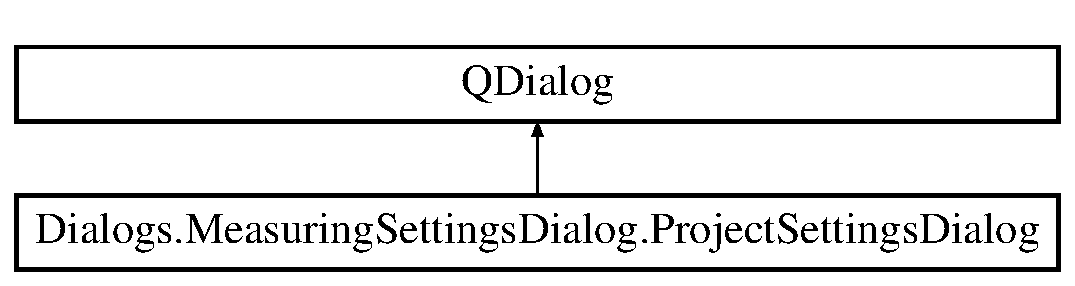
\includegraphics[height=2.000000cm]{classDialogs_1_1MeasuringSettingsDialog_1_1ProjectSettingsDialog}
\end{center}
\end{figure}
\subsection*{Public Member Functions}
\begin{DoxyCompactItemize}
\item 
def \hyperlink{classDialogs_1_1MeasuringSettingsDialog_1_1ProjectSettingsDialog_a603358993a934fdaed3867f9ad43d72f}{\-\_\-\-\_\-init\-\_\-\-\_\-}
\item 
def \hyperlink{classDialogs_1_1MeasuringSettingsDialog_1_1ProjectSettingsDialog_ad5036f7a5b08f5d6024e4d9ba8a027b3}{update\-\_\-and\-\_\-close\-\_\-settings}
\item 
def \hyperlink{classDialogs_1_1MeasuringSettingsDialog_1_1ProjectSettingsDialog_af076d02f49cd614ab600cdc6d0b73289}{update\-\_\-settings}
\end{DoxyCompactItemize}
\subsection*{Public Attributes}
\begin{DoxyCompactItemize}
\item 
\hypertarget{classDialogs_1_1MeasuringSettingsDialog_1_1ProjectSettingsDialog_a21a9081d4a97ce79cff176d32ce73eb8}{{\bfseries ui}}\label{classDialogs_1_1MeasuringSettingsDialog_1_1ProjectSettingsDialog_a21a9081d4a97ce79cff176d32ce73eb8}

\item 
\hypertarget{classDialogs_1_1MeasuringSettingsDialog_1_1ProjectSettingsDialog_afb62061323c5d3a81f2e3bd8ceb79fa2}{{\bfseries masses}}\label{classDialogs_1_1MeasuringSettingsDialog_1_1ProjectSettingsDialog_afb62061323c5d3a81f2e3bd8ceb79fa2}

\item 
\hypertarget{classDialogs_1_1MeasuringSettingsDialog_1_1ProjectSettingsDialog_ad042d099025684db9a6ba89d14e8b6f5}{{\bfseries project}}\label{classDialogs_1_1MeasuringSettingsDialog_1_1ProjectSettingsDialog_ad042d099025684db9a6ba89d14e8b6f5}

\item 
\hypertarget{classDialogs_1_1MeasuringSettingsDialog_1_1ProjectSettingsDialog_a235bc8bb115f116ec06cfd424dfe86eb}{{\bfseries settings}}\label{classDialogs_1_1MeasuringSettingsDialog_1_1ProjectSettingsDialog_a235bc8bb115f116ec06cfd424dfe86eb}

\item 
\hypertarget{classDialogs_1_1MeasuringSettingsDialog_1_1ProjectSettingsDialog_a98a3963fef997e33748792d6d7e57eef}{{\bfseries measuring\-\_\-unit\-\_\-settings}}\label{classDialogs_1_1MeasuringSettingsDialog_1_1ProjectSettingsDialog_a98a3963fef997e33748792d6d7e57eef}

\item 
\hypertarget{classDialogs_1_1MeasuringSettingsDialog_1_1ProjectSettingsDialog_aad607e53762f5479f1f0de2f6be9c285}{{\bfseries calibration\-\_\-settings}}\label{classDialogs_1_1MeasuringSettingsDialog_1_1ProjectSettingsDialog_aad607e53762f5479f1f0de2f6be9c285}

\item 
\hypertarget{classDialogs_1_1MeasuringSettingsDialog_1_1ProjectSettingsDialog_a4257738fd83a49fb39251de27b4ddbd3}{{\bfseries depth\-\_\-profile\-\_\-settings}}\label{classDialogs_1_1MeasuringSettingsDialog_1_1ProjectSettingsDialog_a4257738fd83a49fb39251de27b4ddbd3}

\end{DoxyCompactItemize}


\subsection{Constructor \& Destructor Documentation}
\hypertarget{classDialogs_1_1MeasuringSettingsDialog_1_1ProjectSettingsDialog_a603358993a934fdaed3867f9ad43d72f}{\index{Dialogs\-::\-Measuring\-Settings\-Dialog\-::\-Project\-Settings\-Dialog@{Dialogs\-::\-Measuring\-Settings\-Dialog\-::\-Project\-Settings\-Dialog}!\-\_\-\-\_\-init\-\_\-\-\_\-@{\-\_\-\-\_\-init\-\_\-\-\_\-}}
\index{\-\_\-\-\_\-init\-\_\-\-\_\-@{\-\_\-\-\_\-init\-\_\-\-\_\-}!Dialogs::MeasuringSettingsDialog::ProjectSettingsDialog@{Dialogs\-::\-Measuring\-Settings\-Dialog\-::\-Project\-Settings\-Dialog}}
\subsubsection[{\-\_\-\-\_\-init\-\_\-\-\_\-}]{\setlength{\rightskip}{0pt plus 5cm}def Dialogs.\-Measuring\-Settings\-Dialog.\-Project\-Settings\-Dialog.\-\_\-\-\_\-init\-\_\-\-\_\- (
\begin{DoxyParamCaption}
\item[{}]{self, }
\item[{}]{masses, }
\item[{}]{project}
\end{DoxyParamCaption}
)}}\label{classDialogs_1_1MeasuringSettingsDialog_1_1ProjectSettingsDialog_a603358993a934fdaed3867f9ad43d72f}
\begin{DoxyVerb}Constructor for the program

Args:
    masses: Reference to Masses class object.
    project: Project class object.
\end{DoxyVerb}
 

\subsection{Member Function Documentation}
\hypertarget{classDialogs_1_1MeasuringSettingsDialog_1_1ProjectSettingsDialog_ad5036f7a5b08f5d6024e4d9ba8a027b3}{\index{Dialogs\-::\-Measuring\-Settings\-Dialog\-::\-Project\-Settings\-Dialog@{Dialogs\-::\-Measuring\-Settings\-Dialog\-::\-Project\-Settings\-Dialog}!update\-\_\-and\-\_\-close\-\_\-settings@{update\-\_\-and\-\_\-close\-\_\-settings}}
\index{update\-\_\-and\-\_\-close\-\_\-settings@{update\-\_\-and\-\_\-close\-\_\-settings}!Dialogs::MeasuringSettingsDialog::ProjectSettingsDialog@{Dialogs\-::\-Measuring\-Settings\-Dialog\-::\-Project\-Settings\-Dialog}}
\subsubsection[{update\-\_\-and\-\_\-close\-\_\-settings}]{\setlength{\rightskip}{0pt plus 5cm}def Dialogs.\-Measuring\-Settings\-Dialog.\-Project\-Settings\-Dialog.\-update\-\_\-and\-\_\-close\-\_\-settings (
\begin{DoxyParamCaption}
\item[{}]{self}
\end{DoxyParamCaption}
)}}\label{classDialogs_1_1MeasuringSettingsDialog_1_1ProjectSettingsDialog_ad5036f7a5b08f5d6024e4d9ba8a027b3}
\begin{DoxyVerb}Updates measuring settings values with the dialog's values and saves them
to default ini file.
\end{DoxyVerb}
 \hypertarget{classDialogs_1_1MeasuringSettingsDialog_1_1ProjectSettingsDialog_af076d02f49cd614ab600cdc6d0b73289}{\index{Dialogs\-::\-Measuring\-Settings\-Dialog\-::\-Project\-Settings\-Dialog@{Dialogs\-::\-Measuring\-Settings\-Dialog\-::\-Project\-Settings\-Dialog}!update\-\_\-settings@{update\-\_\-settings}}
\index{update\-\_\-settings@{update\-\_\-settings}!Dialogs::MeasuringSettingsDialog::ProjectSettingsDialog@{Dialogs\-::\-Measuring\-Settings\-Dialog\-::\-Project\-Settings\-Dialog}}
\subsubsection[{update\-\_\-settings}]{\setlength{\rightskip}{0pt plus 5cm}def Dialogs.\-Measuring\-Settings\-Dialog.\-Project\-Settings\-Dialog.\-update\-\_\-settings (
\begin{DoxyParamCaption}
\item[{}]{self}
\end{DoxyParamCaption}
)}}\label{classDialogs_1_1MeasuringSettingsDialog_1_1ProjectSettingsDialog_af076d02f49cd614ab600cdc6d0b73289}
\begin{DoxyVerb}Update values from dialog to every setting object.
\end{DoxyVerb}
 

The documentation for this class was generated from the following file\-:\begin{DoxyCompactItemize}
\item 
Dialogs/Measuring\-Settings\-Dialog.\-py\end{DoxyCompactItemize}

\hypertarget{classModules_1_1Selection_1_1Selection}{\section{Modules.\-Selection.\-Selection Class Reference}
\label{classModules_1_1Selection_1_1Selection}\index{Modules.\-Selection.\-Selection@{Modules.\-Selection.\-Selection}}
}
\subsection*{Public Member Functions}
\begin{DoxyCompactItemize}
\item 
def \hyperlink{classModules_1_1Selection_1_1Selection_a4d921c99a19610c24cccb4bd842af44a}{\-\_\-\-\_\-init\-\_\-\-\_\-}
\item 
def \hyperlink{classModules_1_1Selection_1_1Selection_af2a93edbfe4277ec940d939e97897e57}{add\-\_\-point}
\item 
def \hyperlink{classModules_1_1Selection_1_1Selection_a535a7640e6cc12e9652178160c5ee98d}{undo\-\_\-last}
\item 
def \hyperlink{classModules_1_1Selection_1_1Selection_a9ca3af8c383e55ad57817812a8f615a5}{get\-\_\-points}
\item 
def \hyperlink{classModules_1_1Selection_1_1Selection_a514480f5e8409e4dbd9b2cb3a3833f49}{get\-\_\-first}
\item 
def \hyperlink{classModules_1_1Selection_1_1Selection_a887c36dd384cabbcd212298121cd5902}{get\-\_\-last}
\item 
def \hyperlink{classModules_1_1Selection_1_1Selection_ae345f118be92bdc279539af120c338af}{count}
\item 
def \hyperlink{classModules_1_1Selection_1_1Selection_a4aeff5c923bad8a88892b539672a7843}{end\-\_\-selection}
\item 
def \hyperlink{classModules_1_1Selection_1_1Selection_abe8b7234ad5283109538866ec55cf5d0}{delete}
\item 
def \hyperlink{classModules_1_1Selection_1_1Selection_a106cb30d6f48e711286da425edffa2bf}{draw}
\item 
def \hyperlink{classModules_1_1Selection_1_1Selection_a7e997fbd997e74fb3e0ce9ac03d11d81}{set\-\_\-color}
\item 
def \hyperlink{classModules_1_1Selection_1_1Selection_ab2541bc241efb5e82bab641fea5ce860}{reset\-\_\-color}
\item 
def \hyperlink{classModules_1_1Selection_1_1Selection_a419c19084862d3f29c160c0540a06356}{save\-\_\-string}
\item 
def \hyperlink{classModules_1_1Selection_1_1Selection_ae4f4d863717f7c85453ac9f28bfbb44f}{transpose}
\item 
def \hyperlink{classModules_1_1Selection_1_1Selection_adf363d182b6f41a9a11c0683e27753c3}{get\-\_\-event\-\_\-count}
\item 
def \hyperlink{classModules_1_1Selection_1_1Selection_a777daa5d20d605dbafccd46bec9693ec}{point\-\_\-inside}
\end{DoxyCompactItemize}
\subsection*{Public Attributes}
\begin{DoxyCompactItemize}
\item 
\hypertarget{classModules_1_1Selection_1_1Selection_a429b6786ccb03941146145f79fe32851}{{\bfseries id}}\label{classModules_1_1Selection_1_1Selection_a429b6786ccb03941146145f79fe32851}

\item 
\hypertarget{classModules_1_1Selection_1_1Selection_ab82fd79190493f4f791b4a56583ea2ca}{{\bfseries masses}}\label{classModules_1_1Selection_1_1Selection_ab82fd79190493f4f791b4a56583ea2ca}

\item 
\hypertarget{classModules_1_1Selection_1_1Selection_ab43d5b4bb3e658e55c08c065bce89b45}{{\bfseries element\-\_\-colormap}}\label{classModules_1_1Selection_1_1Selection_ab43d5b4bb3e658e55c08c065bce89b45}

\item 
\hypertarget{classModules_1_1Selection_1_1Selection_a1dff1bc437077385f9e7162949c96f8a}{{\bfseries settings}}\label{classModules_1_1Selection_1_1Selection_a1dff1bc437077385f9e7162949c96f8a}

\item 
\hypertarget{classModules_1_1Selection_1_1Selection_a0c55643f2360be4e5c02a248a4d83f3d}{{\bfseries default\-\_\-color}}\label{classModules_1_1Selection_1_1Selection_a0c55643f2360be4e5c02a248a4d83f3d}

\item 
\hypertarget{classModules_1_1Selection_1_1Selection_a730ee355d9ae0b54eb35139f1a90cdfb}{{\bfseries type}}\label{classModules_1_1Selection_1_1Selection_a730ee355d9ae0b54eb35139f1a90cdfb}

\item 
\hypertarget{classModules_1_1Selection_1_1Selection_adee5376ebdcfc18a9b293c0d3a9fbed0}{{\bfseries element}}\label{classModules_1_1Selection_1_1Selection_adee5376ebdcfc18a9b293c0d3a9fbed0}

\item 
\hypertarget{classModules_1_1Selection_1_1Selection_ab38bb7c007dec78f1e4f64ac586a8b91}{{\bfseries weight\-\_\-factor}}\label{classModules_1_1Selection_1_1Selection_ab38bb7c007dec78f1e4f64ac586a8b91}

\item 
\hypertarget{classModules_1_1Selection_1_1Selection_a63e7a02e0868560917b99a93074de699}{{\bfseries element\-\_\-scatter}}\label{classModules_1_1Selection_1_1Selection_a63e7a02e0868560917b99a93074de699}

\item 
\hypertarget{classModules_1_1Selection_1_1Selection_a98fda495d18126c816b3ceb567e4fda8}{{\bfseries events\-\_\-counted}}\label{classModules_1_1Selection_1_1Selection_a98fda495d18126c816b3ceb567e4fda8}

\item 
\hypertarget{classModules_1_1Selection_1_1Selection_ae6a1e6fc80968bc25e50e0e4dc55cba8}{{\bfseries event\-\_\-count}}\label{classModules_1_1Selection_1_1Selection_ae6a1e6fc80968bc25e50e0e4dc55cba8}

\item 
\hypertarget{classModules_1_1Selection_1_1Selection_a004d7784265603879858a6f886371882}{{\bfseries is\-\_\-closed}}\label{classModules_1_1Selection_1_1Selection_a004d7784265603879858a6f886371882}

\item 
\hypertarget{classModules_1_1Selection_1_1Selection_abfcf853e6b19a3f393dd7393f9e55608}{{\bfseries points}}\label{classModules_1_1Selection_1_1Selection_abfcf853e6b19a3f393dd7393f9e55608}

\item 
\hypertarget{classModules_1_1Selection_1_1Selection_ae803583a13d0b247faed08e506802485}{{\bfseries axes}}\label{classModules_1_1Selection_1_1Selection_ae803583a13d0b247faed08e506802485}

\item 
\hypertarget{classModules_1_1Selection_1_1Selection_aa2860b3c28c618eb55bad1dbcddb3366}{{\bfseries axes\-\_\-limits}}\label{classModules_1_1Selection_1_1Selection_aa2860b3c28c618eb55bad1dbcddb3366}

\end{DoxyCompactItemize}
\subsection*{Static Public Attributes}
\begin{DoxyCompactItemize}
\item 
\hypertarget{classModules_1_1Selection_1_1Selection_a398795a86e970eaab4681dd9ce0ebaad}{string {\bfseries L\-I\-N\-E\-\_\-\-S\-T\-Y\-L\-E} = '-\/'}\label{classModules_1_1Selection_1_1Selection_a398795a86e970eaab4681dd9ce0ebaad}

\item 
\hypertarget{classModules_1_1Selection_1_1Selection_aaf0d83659a4cc3373f2fc46bb9dcf4e6}{string {\bfseries L\-I\-N\-E\-\_\-\-M\-A\-R\-K\-E\-R} = 'o'}\label{classModules_1_1Selection_1_1Selection_aaf0d83659a4cc3373f2fc46bb9dcf4e6}

\item 
\hypertarget{classModules_1_1Selection_1_1Selection_a65a5135ca71ec79e8f87457df10d7737}{float {\bfseries L\-I\-N\-E\-\_\-\-M\-A\-R\-K\-E\-R\-\_\-\-S\-I\-Z\-E} = 3.\-0}\label{classModules_1_1Selection_1_1Selection_a65a5135ca71ec79e8f87457df10d7737}

\item 
\hypertarget{classModules_1_1Selection_1_1Selection_a5558dc889352f0ffb27d585cfe920ebc}{int {\bfseries G\-L\-O\-B\-A\-L\-\_\-\-I\-D} = 0}\label{classModules_1_1Selection_1_1Selection_a5558dc889352f0ffb27d585cfe920ebc}

\end{DoxyCompactItemize}


\subsection{Detailed Description}
\begin{DoxyVerb}Selection object which knows all selection points.
\end{DoxyVerb}
 

\subsection{Constructor \& Destructor Documentation}
\hypertarget{classModules_1_1Selection_1_1Selection_a4d921c99a19610c24cccb4bd842af44a}{\index{Modules\-::\-Selection\-::\-Selection@{Modules\-::\-Selection\-::\-Selection}!\-\_\-\-\_\-init\-\_\-\-\_\-@{\-\_\-\-\_\-init\-\_\-\-\_\-}}
\index{\-\_\-\-\_\-init\-\_\-\-\_\-@{\-\_\-\-\_\-init\-\_\-\-\_\-}!Modules::Selection::Selection@{Modules\-::\-Selection\-::\-Selection}}
\subsubsection[{\-\_\-\-\_\-init\-\_\-\-\_\-}]{\setlength{\rightskip}{0pt plus 5cm}def Modules.\-Selection.\-Selection.\-\_\-\-\_\-init\-\_\-\-\_\- (
\begin{DoxyParamCaption}
\item[{}]{self, }
\item[{}]{axes, }
\item[{}]{masses, }
\item[{}]{element\-\_\-colormap, }
\item[{}]{settings, }
\item[{}]{element = {\ttfamily None}, }
\item[{}]{isotope = {\ttfamily None}, }
\item[{}]{element\-\_\-type = {\ttfamily \char`\"{}ERD\char`\"{}}, }
\item[{}]{color = {\ttfamily None}, }
\item[{}]{points = {\ttfamily None}, }
\item[{}]{scatter = {\ttfamily None}, }
\item[{}]{weight\-\_\-factor = {\ttfamily 1}, }
\item[{}]{transposed = {\ttfamily False}}
\end{DoxyParamCaption}
)}}\label{classModules_1_1Selection_1_1Selection_a4d921c99a19610c24cccb4bd842af44a}
\begin{DoxyVerb}Inits Selection class.

Args:
    axes: Matplotlib FigureCanvas's subplot
    masses: Reference to element masses object of main program.
    element_colormap: Default colors for new element selections.
    settings: Measurement's settings to which selector belongs. 
      (for selection dialog)
    element: String representing element
    isotope: String representing isotope
    element_type: "ERD" or "RBS"
    color: String representing color for the element
    points: String list representing points in selection.
    "X1, X2, X3;Y1, Y2, Y3"
    scatter: String representing scatter element. 
    weight_factor: Weight factor for the element.
    transposed: Boolean representing if axes are transposed.
\end{DoxyVerb}
 

\subsection{Member Function Documentation}
\hypertarget{classModules_1_1Selection_1_1Selection_af2a93edbfe4277ec940d939e97897e57}{\index{Modules\-::\-Selection\-::\-Selection@{Modules\-::\-Selection\-::\-Selection}!add\-\_\-point@{add\-\_\-point}}
\index{add\-\_\-point@{add\-\_\-point}!Modules::Selection::Selection@{Modules\-::\-Selection\-::\-Selection}}
\subsubsection[{add\-\_\-point}]{\setlength{\rightskip}{0pt plus 5cm}def Modules.\-Selection.\-Selection.\-add\-\_\-point (
\begin{DoxyParamCaption}
\item[{}]{self, }
\item[{}]{point}
\end{DoxyParamCaption}
)}}\label{classModules_1_1Selection_1_1Selection_af2a93edbfe4277ec940d939e97897e57}
\begin{DoxyVerb}Adds a point to selection.

Adds a point to selection. If selection is closed, do nothing.

Args:
    point: Point (x, y) to be added to selection.

Return:
    0: Point was added.
    -1: If selection is closed.
\end{DoxyVerb}
 \hypertarget{classModules_1_1Selection_1_1Selection_ae345f118be92bdc279539af120c338af}{\index{Modules\-::\-Selection\-::\-Selection@{Modules\-::\-Selection\-::\-Selection}!count@{count}}
\index{count@{count}!Modules::Selection::Selection@{Modules\-::\-Selection\-::\-Selection}}
\subsubsection[{count}]{\setlength{\rightskip}{0pt plus 5cm}def Modules.\-Selection.\-Selection.\-count (
\begin{DoxyParamCaption}
\item[{}]{self}
\end{DoxyParamCaption}
)}}\label{classModules_1_1Selection_1_1Selection_ae345f118be92bdc279539af120c338af}
\begin{DoxyVerb}Get the count of node points in selection.

Return
    Returns the count of node points in selection.
\end{DoxyVerb}
 \hypertarget{classModules_1_1Selection_1_1Selection_abe8b7234ad5283109538866ec55cf5d0}{\index{Modules\-::\-Selection\-::\-Selection@{Modules\-::\-Selection\-::\-Selection}!delete@{delete}}
\index{delete@{delete}!Modules::Selection::Selection@{Modules\-::\-Selection\-::\-Selection}}
\subsubsection[{delete}]{\setlength{\rightskip}{0pt plus 5cm}def Modules.\-Selection.\-Selection.\-delete (
\begin{DoxyParamCaption}
\item[{}]{self}
\end{DoxyParamCaption}
)}}\label{classModules_1_1Selection_1_1Selection_abe8b7234ad5283109538866ec55cf5d0}
\begin{DoxyVerb}Delete this selection.
\end{DoxyVerb}
 \hypertarget{classModules_1_1Selection_1_1Selection_a106cb30d6f48e711286da425edffa2bf}{\index{Modules\-::\-Selection\-::\-Selection@{Modules\-::\-Selection\-::\-Selection}!draw@{draw}}
\index{draw@{draw}!Modules::Selection::Selection@{Modules\-::\-Selection\-::\-Selection}}
\subsubsection[{draw}]{\setlength{\rightskip}{0pt plus 5cm}def Modules.\-Selection.\-Selection.\-draw (
\begin{DoxyParamCaption}
\item[{}]{self}
\end{DoxyParamCaption}
)}}\label{classModules_1_1Selection_1_1Selection_a106cb30d6f48e711286da425edffa2bf}
\begin{DoxyVerb}Draw selection points into graph (matplotlib) axes
\end{DoxyVerb}
 \hypertarget{classModules_1_1Selection_1_1Selection_a4aeff5c923bad8a88892b539672a7843}{\index{Modules\-::\-Selection\-::\-Selection@{Modules\-::\-Selection\-::\-Selection}!end\-\_\-selection@{end\-\_\-selection}}
\index{end\-\_\-selection@{end\-\_\-selection}!Modules::Selection::Selection@{Modules\-::\-Selection\-::\-Selection}}
\subsubsection[{end\-\_\-selection}]{\setlength{\rightskip}{0pt plus 5cm}def Modules.\-Selection.\-Selection.\-end\-\_\-selection (
\begin{DoxyParamCaption}
\item[{}]{self, }
\item[{}]{canvas = {\ttfamily None}}
\end{DoxyParamCaption}
)}}\label{classModules_1_1Selection_1_1Selection_a4aeff5c923bad8a88892b539672a7843}
\begin{DoxyVerb}End selection.

Ends selection. If selection is open and canvas is not None, it will 
show dialog to select element information and draws into canvas 
before opening the dialog.

Args:
    canvas: Matplotlib's FigureCanvas or None when we don't want 
    to new selection window. None, when loading selections 
    so we do not want to open new selection settings dialog.

Return:
    True: Selection was completed
    False: Selection settings was not set (cancel button)
\end{DoxyVerb}
 \hypertarget{classModules_1_1Selection_1_1Selection_adf363d182b6f41a9a11c0683e27753c3}{\index{Modules\-::\-Selection\-::\-Selection@{Modules\-::\-Selection\-::\-Selection}!get\-\_\-event\-\_\-count@{get\-\_\-event\-\_\-count}}
\index{get\-\_\-event\-\_\-count@{get\-\_\-event\-\_\-count}!Modules::Selection::Selection@{Modules\-::\-Selection\-::\-Selection}}
\subsubsection[{get\-\_\-event\-\_\-count}]{\setlength{\rightskip}{0pt plus 5cm}def Modules.\-Selection.\-Selection.\-get\-\_\-event\-\_\-count (
\begin{DoxyParamCaption}
\item[{}]{self}
\end{DoxyParamCaption}
)}}\label{classModules_1_1Selection_1_1Selection_adf363d182b6f41a9a11c0683e27753c3}
\begin{DoxyVerb}Get the count of event points within the selection.

Return:
    Returns an integer representing the count of event points within 
    the selection.
\end{DoxyVerb}
 \hypertarget{classModules_1_1Selection_1_1Selection_a514480f5e8409e4dbd9b2cb3a3833f49}{\index{Modules\-::\-Selection\-::\-Selection@{Modules\-::\-Selection\-::\-Selection}!get\-\_\-first@{get\-\_\-first}}
\index{get\-\_\-first@{get\-\_\-first}!Modules::Selection::Selection@{Modules\-::\-Selection\-::\-Selection}}
\subsubsection[{get\-\_\-first}]{\setlength{\rightskip}{0pt plus 5cm}def Modules.\-Selection.\-Selection.\-get\-\_\-first (
\begin{DoxyParamCaption}
\item[{}]{self}
\end{DoxyParamCaption}
)}}\label{classModules_1_1Selection_1_1Selection_a514480f5e8409e4dbd9b2cb3a3833f49}
\begin{DoxyVerb}Get first point in selection

Return:
    None: If no point in selection
    (x, y): Otherwise
\end{DoxyVerb}
 \hypertarget{classModules_1_1Selection_1_1Selection_a887c36dd384cabbcd212298121cd5902}{\index{Modules\-::\-Selection\-::\-Selection@{Modules\-::\-Selection\-::\-Selection}!get\-\_\-last@{get\-\_\-last}}
\index{get\-\_\-last@{get\-\_\-last}!Modules::Selection::Selection@{Modules\-::\-Selection\-::\-Selection}}
\subsubsection[{get\-\_\-last}]{\setlength{\rightskip}{0pt plus 5cm}def Modules.\-Selection.\-Selection.\-get\-\_\-last (
\begin{DoxyParamCaption}
\item[{}]{self}
\end{DoxyParamCaption}
)}}\label{classModules_1_1Selection_1_1Selection_a887c36dd384cabbcd212298121cd5902}
\begin{DoxyVerb}Get last point in selection

Return:
    None: If no point in selection
    (x, y): Otherwise
\end{DoxyVerb}
 \hypertarget{classModules_1_1Selection_1_1Selection_a9ca3af8c383e55ad57817812a8f615a5}{\index{Modules\-::\-Selection\-::\-Selection@{Modules\-::\-Selection\-::\-Selection}!get\-\_\-points@{get\-\_\-points}}
\index{get\-\_\-points@{get\-\_\-points}!Modules::Selection::Selection@{Modules\-::\-Selection\-::\-Selection}}
\subsubsection[{get\-\_\-points}]{\setlength{\rightskip}{0pt plus 5cm}def Modules.\-Selection.\-Selection.\-get\-\_\-points (
\begin{DoxyParamCaption}
\item[{}]{self}
\end{DoxyParamCaption}
)}}\label{classModules_1_1Selection_1_1Selection_a9ca3af8c383e55ad57817812a8f615a5}
\begin{DoxyVerb}Get points in selection 

Get points in selection in list. Format: ((x1,y1), (x2,y2), ...). 
If no points, empty list is returned

Return:
   ((x1, y1), (x2, y2), ...)
\end{DoxyVerb}
 \hypertarget{classModules_1_1Selection_1_1Selection_a777daa5d20d605dbafccd46bec9693ec}{\index{Modules\-::\-Selection\-::\-Selection@{Modules\-::\-Selection\-::\-Selection}!point\-\_\-inside@{point\-\_\-inside}}
\index{point\-\_\-inside@{point\-\_\-inside}!Modules::Selection::Selection@{Modules\-::\-Selection\-::\-Selection}}
\subsubsection[{point\-\_\-inside}]{\setlength{\rightskip}{0pt plus 5cm}def Modules.\-Selection.\-Selection.\-point\-\_\-inside (
\begin{DoxyParamCaption}
\item[{}]{self, }
\item[{}]{point}
\end{DoxyParamCaption}
)}}\label{classModules_1_1Selection_1_1Selection_a777daa5d20d605dbafccd46bec9693ec}
\begin{DoxyVerb}Check if point is inside selection.

Args:
    point: [X, Y] representing a point.
    
Return:
    Returns True if point is within selection. False otherwise.
\end{DoxyVerb}
 \hypertarget{classModules_1_1Selection_1_1Selection_ab2541bc241efb5e82bab641fea5ce860}{\index{Modules\-::\-Selection\-::\-Selection@{Modules\-::\-Selection\-::\-Selection}!reset\-\_\-color@{reset\-\_\-color}}
\index{reset\-\_\-color@{reset\-\_\-color}!Modules::Selection::Selection@{Modules\-::\-Selection\-::\-Selection}}
\subsubsection[{reset\-\_\-color}]{\setlength{\rightskip}{0pt plus 5cm}def Modules.\-Selection.\-Selection.\-reset\-\_\-color (
\begin{DoxyParamCaption}
\item[{}]{self}
\end{DoxyParamCaption}
)}}\label{classModules_1_1Selection_1_1Selection_ab2541bc241efb5e82bab641fea5ce860}
\begin{DoxyVerb}Reset selection color to default color.
\end{DoxyVerb}
 \hypertarget{classModules_1_1Selection_1_1Selection_a419c19084862d3f29c160c0540a06356}{\index{Modules\-::\-Selection\-::\-Selection@{Modules\-::\-Selection\-::\-Selection}!save\-\_\-string@{save\-\_\-string}}
\index{save\-\_\-string@{save\-\_\-string}!Modules::Selection::Selection@{Modules\-::\-Selection\-::\-Selection}}
\subsubsection[{save\-\_\-string}]{\setlength{\rightskip}{0pt plus 5cm}def Modules.\-Selection.\-Selection.\-save\-\_\-string (
\begin{DoxyParamCaption}
\item[{}]{self, }
\item[{}]{is\-\_\-transposed}
\end{DoxyParamCaption}
)}}\label{classModules_1_1Selection_1_1Selection_a419c19084862d3f29c160c0540a06356}
\begin{DoxyVerb}Get selection in string format for selectiong file save.

Args:
    is_transposed: Boolean representing if axes are transposed.
    
Return:
    String representing current selection object.
\end{DoxyVerb}
 \hypertarget{classModules_1_1Selection_1_1Selection_a7e997fbd997e74fb3e0ce9ac03d11d81}{\index{Modules\-::\-Selection\-::\-Selection@{Modules\-::\-Selection\-::\-Selection}!set\-\_\-color@{set\-\_\-color}}
\index{set\-\_\-color@{set\-\_\-color}!Modules::Selection::Selection@{Modules\-::\-Selection\-::\-Selection}}
\subsubsection[{set\-\_\-color}]{\setlength{\rightskip}{0pt plus 5cm}def Modules.\-Selection.\-Selection.\-set\-\_\-color (
\begin{DoxyParamCaption}
\item[{}]{self, }
\item[{}]{color}
\end{DoxyParamCaption}
)}}\label{classModules_1_1Selection_1_1Selection_a7e997fbd997e74fb3e0ce9ac03d11d81}
\begin{DoxyVerb}Set selection color

Args:
    color: String representing color. 
   Format is whatever QtGui.QColor(string) understands.
\end{DoxyVerb}
 \hypertarget{classModules_1_1Selection_1_1Selection_ae4f4d863717f7c85453ac9f28bfbb44f}{\index{Modules\-::\-Selection\-::\-Selection@{Modules\-::\-Selection\-::\-Selection}!transpose@{transpose}}
\index{transpose@{transpose}!Modules::Selection::Selection@{Modules\-::\-Selection\-::\-Selection}}
\subsubsection[{transpose}]{\setlength{\rightskip}{0pt plus 5cm}def Modules.\-Selection.\-Selection.\-transpose (
\begin{DoxyParamCaption}
\item[{}]{self, }
\item[{}]{transpose}
\end{DoxyParamCaption}
)}}\label{classModules_1_1Selection_1_1Selection_ae4f4d863717f7c85453ac9f28bfbb44f}
\begin{DoxyVerb}Transpose selection points.

Args:
    transpose: Boolean representing whether to transpose selection points.
\end{DoxyVerb}
 \hypertarget{classModules_1_1Selection_1_1Selection_a535a7640e6cc12e9652178160c5ee98d}{\index{Modules\-::\-Selection\-::\-Selection@{Modules\-::\-Selection\-::\-Selection}!undo\-\_\-last@{undo\-\_\-last}}
\index{undo\-\_\-last@{undo\-\_\-last}!Modules::Selection::Selection@{Modules\-::\-Selection\-::\-Selection}}
\subsubsection[{undo\-\_\-last}]{\setlength{\rightskip}{0pt plus 5cm}def Modules.\-Selection.\-Selection.\-undo\-\_\-last (
\begin{DoxyParamCaption}
\item[{}]{self}
\end{DoxyParamCaption}
)}}\label{classModules_1_1Selection_1_1Selection_a535a7640e6cc12e9652178160c5ee98d}
\begin{DoxyVerb}Undo last point in selection.

Return:
    1: If selection is closed or there are no points in selection.
    0: If everything is ok.
\end{DoxyVerb}
 

The documentation for this class was generated from the following file\-:\begin{DoxyCompactItemize}
\item 
Modules/Selection.\-py\end{DoxyCompactItemize}

\hypertarget{classDialogs_1_1SelectionDialog_1_1SelectionSettingsDialog}{\section{Dialogs.\-Selection\-Dialog.\-Selection\-Settings\-Dialog Class Reference}
\label{classDialogs_1_1SelectionDialog_1_1SelectionSettingsDialog}\index{Dialogs.\-Selection\-Dialog.\-Selection\-Settings\-Dialog@{Dialogs.\-Selection\-Dialog.\-Selection\-Settings\-Dialog}}
}
Inheritance diagram for Dialogs.\-Selection\-Dialog.\-Selection\-Settings\-Dialog\-:\begin{figure}[H]
\begin{center}
\leavevmode
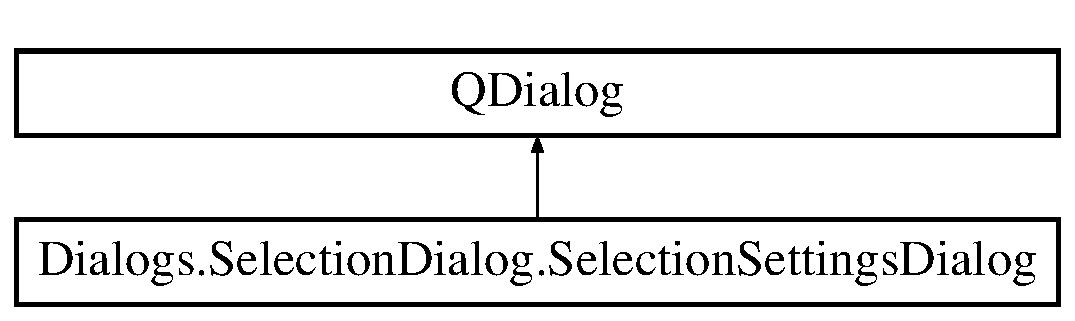
\includegraphics[height=2.000000cm]{classDialogs_1_1SelectionDialog_1_1SelectionSettingsDialog}
\end{center}
\end{figure}
\subsection*{Public Member Functions}
\begin{DoxyCompactItemize}
\item 
def \hyperlink{classDialogs_1_1SelectionDialog_1_1SelectionSettingsDialog_a4c52181a16d7934d1c1e6a3b00e066be}{\-\_\-\-\_\-init\-\_\-\-\_\-}
\end{DoxyCompactItemize}
\subsection*{Public Attributes}
\begin{DoxyCompactItemize}
\item 
\hypertarget{classDialogs_1_1SelectionDialog_1_1SelectionSettingsDialog_aca90625a206f72c6cf9c4d64c8f4ac29}{{\bfseries selection}}\label{classDialogs_1_1SelectionDialog_1_1SelectionSettingsDialog_aca90625a206f72c6cf9c4d64c8f4ac29}

\item 
\hypertarget{classDialogs_1_1SelectionDialog_1_1SelectionSettingsDialog_a4387c416279f64c1b13290fc3d92f845}{{\bfseries settings}}\label{classDialogs_1_1SelectionDialog_1_1SelectionSettingsDialog_a4387c416279f64c1b13290fc3d92f845}

\item 
\hypertarget{classDialogs_1_1SelectionDialog_1_1SelectionSettingsDialog_a97c3f3c37e91924b6fa7cfe7c1b7d731}{{\bfseries element\-\_\-colormap}}\label{classDialogs_1_1SelectionDialog_1_1SelectionSettingsDialog_a97c3f3c37e91924b6fa7cfe7c1b7d731}

\item 
\hypertarget{classDialogs_1_1SelectionDialog_1_1SelectionSettingsDialog_a8a57a64137f5a2c41b3e7399c43b239f}{{\bfseries ui}}\label{classDialogs_1_1SelectionDialog_1_1SelectionSettingsDialog_a8a57a64137f5a2c41b3e7399c43b239f}

\item 
\hypertarget{classDialogs_1_1SelectionDialog_1_1SelectionSettingsDialog_a74b880557e46d672aaab2b722f48e37a}{{\bfseries is\-Ok}}\label{classDialogs_1_1SelectionDialog_1_1SelectionSettingsDialog_a74b880557e46d672aaab2b722f48e37a}

\item 
\hypertarget{classDialogs_1_1SelectionDialog_1_1SelectionSettingsDialog_a241ec2cb90771555d113d12c7b65023c}{{\bfseries color}}\label{classDialogs_1_1SelectionDialog_1_1SelectionSettingsDialog_a241ec2cb90771555d113d12c7b65023c}

\end{DoxyCompactItemize}


\subsection{Detailed Description}
\begin{DoxyVerb}Selection Settings dialog handles showing settings for selection made in 
measurement (in matplotlib graph).
\end{DoxyVerb}
 

\subsection{Constructor \& Destructor Documentation}
\hypertarget{classDialogs_1_1SelectionDialog_1_1SelectionSettingsDialog_a4c52181a16d7934d1c1e6a3b00e066be}{\index{Dialogs\-::\-Selection\-Dialog\-::\-Selection\-Settings\-Dialog@{Dialogs\-::\-Selection\-Dialog\-::\-Selection\-Settings\-Dialog}!\-\_\-\-\_\-init\-\_\-\-\_\-@{\-\_\-\-\_\-init\-\_\-\-\_\-}}
\index{\-\_\-\-\_\-init\-\_\-\-\_\-@{\-\_\-\-\_\-init\-\_\-\-\_\-}!Dialogs::SelectionDialog::SelectionSettingsDialog@{Dialogs\-::\-Selection\-Dialog\-::\-Selection\-Settings\-Dialog}}
\subsubsection[{\-\_\-\-\_\-init\-\_\-\-\_\-}]{\setlength{\rightskip}{0pt plus 5cm}def Dialogs.\-Selection\-Dialog.\-Selection\-Settings\-Dialog.\-\_\-\-\_\-init\-\_\-\-\_\- (
\begin{DoxyParamCaption}
\item[{}]{self, }
\item[{}]{selection}
\end{DoxyParamCaption}
)}}\label{classDialogs_1_1SelectionDialog_1_1SelectionSettingsDialog_a4c52181a16d7934d1c1e6a3b00e066be}
\begin{DoxyVerb}Inits selection settings dialog.

Args:
    selection: Selection class object.
\end{DoxyVerb}
 

The documentation for this class was generated from the following file\-:\begin{DoxyCompactItemize}
\item 
Dialogs/Selection\-Dialog.\-py\end{DoxyCompactItemize}

\hypertarget{classModules_1_1Selection_1_1Selector}{\section{Modules.\-Selection.\-Selector Class Reference}
\label{classModules_1_1Selection_1_1Selector}\index{Modules.\-Selection.\-Selector@{Modules.\-Selection.\-Selector}}
}
\subsection*{Public Member Functions}
\begin{DoxyCompactItemize}
\item 
def \hyperlink{classModules_1_1Selection_1_1Selector_a1b98af1f25e688e011b503940f8d9d38}{\-\_\-\-\_\-init\-\_\-\-\_\-}
\item 
def \hyperlink{classModules_1_1Selection_1_1Selector_a57f1e6c1d88b595d11a9a4a9b81f6c2b}{count}
\item 
def \hyperlink{classModules_1_1Selection_1_1Selector_a3062c36cd70a61b57dba62b2aa7deae3}{is\-\_\-empty}
\item 
def \hyperlink{classModules_1_1Selection_1_1Selector_a76c0b484dd4960f572ac097cc6a9018f}{get\-\_\-at}
\item 
def \hyperlink{classModules_1_1Selection_1_1Selector_a8cb517933be366669b37554ae22ea022}{get\-\_\-selected}
\item 
def \hyperlink{classModules_1_1Selection_1_1Selector_accfcafb39c5fa5fcf1ff5c1da1d43461}{add\-\_\-point}
\item 
def \hyperlink{classModules_1_1Selection_1_1Selector_abeceee26df62e70817d924b6323bebfe}{undo\-\_\-point}
\item 
def \hyperlink{classModules_1_1Selection_1_1Selector_a286ace8f8487fdad80fb46eb6b645086}{purge}
\item 
def \hyperlink{classModules_1_1Selection_1_1Selector_af0c515145afa4fff51d7b061d42898b0}{remove\-\_\-selected}
\item 
def \hyperlink{classModules_1_1Selection_1_1Selector_a22b452174c86921942a6ed010b4b6748}{remove\-\_\-all}
\item 
def \hyperlink{classModules_1_1Selection_1_1Selector_ac6821be9818506f78ebc0263ce0cb8fa}{distance}
\item 
def \hyperlink{classModules_1_1Selection_1_1Selector_a5bf9ee3a076b7b6153dc4f2a84665be8}{draw}
\item 
def \hyperlink{classModules_1_1Selection_1_1Selector_a75dd39a943e05f1fce458b3feb56d834}{end\-\_\-open\-\_\-selection}
\item 
def \hyperlink{classModules_1_1Selection_1_1Selector_a773c514f0089ddf5c057b925756aa7df}{select}
\item 
def \hyperlink{classModules_1_1Selection_1_1Selector_a86dca218c5925c039f043d8a6c4ac2a0}{reset\-\_\-select}
\item 
def \hyperlink{classModules_1_1Selection_1_1Selector_acc5edd2eccc27a9d568a460825d5f0df}{reset\-\_\-colors}
\item 
def \hyperlink{classModules_1_1Selection_1_1Selector_ac0d83b3bbc909098f895e9091dfb3dc2}{get\-\_\-colors}
\item 
def \hyperlink{classModules_1_1Selection_1_1Selector_a522a482a5a06c27be58b6536ad313d18}{grey\-\_\-out\-\_\-except}
\item 
def \hyperlink{classModules_1_1Selection_1_1Selector_abb805a39768ab091c5aa82292fe9a598}{auto\-\_\-save}
\item 
def \hyperlink{classModules_1_1Selection_1_1Selector_a3a1b957e229d6df197a646fb644462bc}{load}
\item 
def \hyperlink{classModules_1_1Selection_1_1Selector_ad15da1910bf79b7f47e4b191ea110145}{update\-\_\-axes\-\_\-limits}
\item 
def \hyperlink{classModules_1_1Selection_1_1Selector_acbcd93aa4d2fa456b540473789975d41}{transpose}
\item 
\hypertarget{classModules_1_1Selection_1_1Selector_ae6b76aa003b906bbe20c2d6a1e39ed28}{def {\bfseries update\-\_\-single\-\_\-selection\-\_\-points}}\label{classModules_1_1Selection_1_1Selector_ae6b76aa003b906bbe20c2d6a1e39ed28}

\item 
def \hyperlink{classModules_1_1Selection_1_1Selector_adba81b4dad3311cadcef43ac92cefc00}{update\-\_\-selection\-\_\-points}
\end{DoxyCompactItemize}
\subsection*{Public Attributes}
\begin{DoxyCompactItemize}
\item 
\hypertarget{classModules_1_1Selection_1_1Selector_a865e963bca3b5d8b4d5d16ffe2b1fbe5}{{\bfseries element\-\_\-colormap}}\label{classModules_1_1Selection_1_1Selector_a865e963bca3b5d8b4d5d16ffe2b1fbe5}

\item 
\hypertarget{classModules_1_1Selection_1_1Selector_ab20eea30f00b051f84b46d9019f428de}{{\bfseries settings}}\label{classModules_1_1Selection_1_1Selector_ab20eea30f00b051f84b46d9019f428de}

\item 
\hypertarget{classModules_1_1Selection_1_1Selector_a6f372d3007b85a8e447b8d73208a8c38}{{\bfseries measurement\-\_\-name}}\label{classModules_1_1Selection_1_1Selector_a6f372d3007b85a8e447b8d73208a8c38}

\item 
\hypertarget{classModules_1_1Selection_1_1Selector_a077b2ad9394ab54dbb7504c744007e62}{{\bfseries directory}}\label{classModules_1_1Selection_1_1Selector_a077b2ad9394ab54dbb7504c744007e62}

\item 
\hypertarget{classModules_1_1Selection_1_1Selector_ac4404f686350b280439e0f3acc377897}{{\bfseries selection\-\_\-file}}\label{classModules_1_1Selection_1_1Selector_ac4404f686350b280439e0f3acc377897}

\item 
\hypertarget{classModules_1_1Selection_1_1Selector_a05a8fa802e1b0eba37da3c862417a896}{{\bfseries selections}}\label{classModules_1_1Selection_1_1Selector_a05a8fa802e1b0eba37da3c862417a896}

\item 
\hypertarget{classModules_1_1Selection_1_1Selector_aaaf72ac7a01c69dfb75ca4b4f03084b8}{{\bfseries new\-\_\-selection\-\_\-is\-\_\-allowed}}\label{classModules_1_1Selection_1_1Selector_aaaf72ac7a01c69dfb75ca4b4f03084b8}

\item 
\hypertarget{classModules_1_1Selection_1_1Selector_a942cb58820d529e7f6351b9bc01a4f57}{{\bfseries is\-\_\-transposed}}\label{classModules_1_1Selection_1_1Selector_a942cb58820d529e7f6351b9bc01a4f57}

\item 
\hypertarget{classModules_1_1Selection_1_1Selector_a6db93acae3982bcd6ecc6ed59f64e539}{{\bfseries looseness}}\label{classModules_1_1Selection_1_1Selector_a6db93acae3982bcd6ecc6ed59f64e539}

\item 
\hypertarget{classModules_1_1Selection_1_1Selector_ace6730171ad28c205cce42cc2d5c0623}{{\bfseries axes}}\label{classModules_1_1Selection_1_1Selector_ace6730171ad28c205cce42cc2d5c0623}

\item 
\hypertarget{classModules_1_1Selection_1_1Selector_af84047b4e4fea7995ef48d4590ad0462}{{\bfseries axes\-\_\-limits}}\label{classModules_1_1Selection_1_1Selector_af84047b4e4fea7995ef48d4590ad0462}

\item 
\hypertarget{classModules_1_1Selection_1_1Selector_ab6916839df1610b7c1a9161840fcfd7f}{{\bfseries selected\-\_\-id}}\label{classModules_1_1Selection_1_1Selector_ab6916839df1610b7c1a9161840fcfd7f}

\item 
\hypertarget{classModules_1_1Selection_1_1Selector_ae0390ab9d1fa7e3f6f3afb14a21c71af}{{\bfseries draw\-\_\-legend}}\label{classModules_1_1Selection_1_1Selector_ae0390ab9d1fa7e3f6f3afb14a21c71af}

\item 
\hypertarget{classModules_1_1Selection_1_1Selector_ac536aee139872904f170f2126ad88c8b}{{\bfseries masses}}\label{classModules_1_1Selection_1_1Selector_ac536aee139872904f170f2126ad88c8b}

\end{DoxyCompactItemize}


\subsection{Detailed Description}
\begin{DoxyVerb}Selector objects handles all selections within measurement.
\end{DoxyVerb}
 

\subsection{Constructor \& Destructor Documentation}
\hypertarget{classModules_1_1Selection_1_1Selector_a1b98af1f25e688e011b503940f8d9d38}{\index{Modules\-::\-Selection\-::\-Selector@{Modules\-::\-Selection\-::\-Selector}!\-\_\-\-\_\-init\-\_\-\-\_\-@{\-\_\-\-\_\-init\-\_\-\-\_\-}}
\index{\-\_\-\-\_\-init\-\_\-\-\_\-@{\-\_\-\-\_\-init\-\_\-\-\_\-}!Modules::Selection::Selector@{Modules\-::\-Selection\-::\-Selector}}
\subsubsection[{\-\_\-\-\_\-init\-\_\-\-\_\-}]{\setlength{\rightskip}{0pt plus 5cm}def Modules.\-Selection.\-Selector.\-\_\-\-\_\-init\-\_\-\-\_\- (
\begin{DoxyParamCaption}
\item[{}]{self, }
\item[{}]{directory, }
\item[{}]{measurement\-\_\-name, }
\item[{}]{masses, }
\item[{}]{element\-\_\-colormap, }
\item[{}]{settings}
\end{DoxyParamCaption}
)}}\label{classModules_1_1Selection_1_1Selector_a1b98af1f25e688e011b503940f8d9d38}
\begin{DoxyVerb}Inits Selector.

Inits Selector object.

Args:
    filepath: String representing filepath of measurement data (ascii file).
    masses: Reference to element masses object of main program.
    element_colormap: Default colors for new element selections.
    settings: Measurement's settings to which selector belongs. 
      (for selection dialog)
\end{DoxyVerb}
 

\subsection{Member Function Documentation}
\hypertarget{classModules_1_1Selection_1_1Selector_accfcafb39c5fa5fcf1ff5c1da1d43461}{\index{Modules\-::\-Selection\-::\-Selector@{Modules\-::\-Selection\-::\-Selector}!add\-\_\-point@{add\-\_\-point}}
\index{add\-\_\-point@{add\-\_\-point}!Modules::Selection::Selector@{Modules\-::\-Selection\-::\-Selector}}
\subsubsection[{add\-\_\-point}]{\setlength{\rightskip}{0pt plus 5cm}def Modules.\-Selection.\-Selector.\-add\-\_\-point (
\begin{DoxyParamCaption}
\item[{}]{self, }
\item[{}]{point, }
\item[{}]{canvas}
\end{DoxyParamCaption}
)}}\label{classModules_1_1Selection_1_1Selector_accfcafb39c5fa5fcf1ff5c1da1d43461}
\begin{DoxyVerb}Adds a new point.

Adds a new point to last selection. If new selection is allowed, create
a new selection to which point is added. If point is in close proximity
of first point in (last) Selection, then close selection and allow new 
selection to be made.

Args:
    point: Point (x, y) to be added to selection.
    canvas: matplotlib's FigureCanvas where selections are drawn.
    
Return:
    1: When point closes open selection and allows new selection to 
be made.
    0: When point was added to open selection.
    -1: When new selection is not allowed and there are no selections.
\end{DoxyVerb}
 \hypertarget{classModules_1_1Selection_1_1Selector_abb805a39768ab091c5aa82292fe9a598}{\index{Modules\-::\-Selection\-::\-Selector@{Modules\-::\-Selection\-::\-Selector}!auto\-\_\-save@{auto\-\_\-save}}
\index{auto\-\_\-save@{auto\-\_\-save}!Modules::Selection::Selector@{Modules\-::\-Selection\-::\-Selector}}
\subsubsection[{auto\-\_\-save}]{\setlength{\rightskip}{0pt plus 5cm}def Modules.\-Selection.\-Selector.\-auto\-\_\-save (
\begin{DoxyParamCaption}
\item[{}]{self}
\end{DoxyParamCaption}
)}}\label{classModules_1_1Selection_1_1Selector_abb805a39768ab091c5aa82292fe9a598}
\begin{DoxyVerb}Save all selections into a file.
\end{DoxyVerb}
 \hypertarget{classModules_1_1Selection_1_1Selector_a57f1e6c1d88b595d11a9a4a9b81f6c2b}{\index{Modules\-::\-Selection\-::\-Selector@{Modules\-::\-Selection\-::\-Selector}!count@{count}}
\index{count@{count}!Modules::Selection::Selector@{Modules\-::\-Selection\-::\-Selector}}
\subsubsection[{count}]{\setlength{\rightskip}{0pt plus 5cm}def Modules.\-Selection.\-Selector.\-count (
\begin{DoxyParamCaption}
\item[{}]{self}
\end{DoxyParamCaption}
)}}\label{classModules_1_1Selection_1_1Selector_a57f1e6c1d88b595d11a9a4a9b81f6c2b}
\begin{DoxyVerb}Get count of selections.

Return:
    Returns the count of selections in selector object.
\end{DoxyVerb}
 \hypertarget{classModules_1_1Selection_1_1Selector_ac6821be9818506f78ebc0263ce0cb8fa}{\index{Modules\-::\-Selection\-::\-Selector@{Modules\-::\-Selection\-::\-Selector}!distance@{distance}}
\index{distance@{distance}!Modules::Selection::Selector@{Modules\-::\-Selection\-::\-Selector}}
\subsubsection[{distance}]{\setlength{\rightskip}{0pt plus 5cm}def Modules.\-Selection.\-Selector.\-distance (
\begin{DoxyParamCaption}
\item[{}]{self, }
\item[{}]{p0, }
\item[{}]{p1}
\end{DoxyParamCaption}
)}}\label{classModules_1_1Selection_1_1Selector_ac6821be9818506f78ebc0263ce0cb8fa}
\begin{DoxyVerb}Distance between points

Calculates and returns distance between two points.

Args:
    p0: Point A
    p1: Point B

Return:
    Distance (float) between two points.
\end{DoxyVerb}
 \hypertarget{classModules_1_1Selection_1_1Selector_a5bf9ee3a076b7b6153dc4f2a84665be8}{\index{Modules\-::\-Selection\-::\-Selector@{Modules\-::\-Selection\-::\-Selector}!draw@{draw}}
\index{draw@{draw}!Modules::Selection::Selector@{Modules\-::\-Selection\-::\-Selector}}
\subsubsection[{draw}]{\setlength{\rightskip}{0pt plus 5cm}def Modules.\-Selection.\-Selector.\-draw (
\begin{DoxyParamCaption}
\item[{}]{self}
\end{DoxyParamCaption}
)}}\label{classModules_1_1Selection_1_1Selector_a5bf9ee3a076b7b6153dc4f2a84665be8}
\begin{DoxyVerb}Draw selections.

Issue draw to all selections in selector.
\end{DoxyVerb}
 \hypertarget{classModules_1_1Selection_1_1Selector_a75dd39a943e05f1fce458b3feb56d834}{\index{Modules\-::\-Selection\-::\-Selector@{Modules\-::\-Selection\-::\-Selector}!end\-\_\-open\-\_\-selection@{end\-\_\-open\-\_\-selection}}
\index{end\-\_\-open\-\_\-selection@{end\-\_\-open\-\_\-selection}!Modules::Selection::Selector@{Modules\-::\-Selection\-::\-Selector}}
\subsubsection[{end\-\_\-open\-\_\-selection}]{\setlength{\rightskip}{0pt plus 5cm}def Modules.\-Selection.\-Selector.\-end\-\_\-open\-\_\-selection (
\begin{DoxyParamCaption}
\item[{}]{self, }
\item[{}]{canvas}
\end{DoxyParamCaption}
)}}\label{classModules_1_1Selection_1_1Selector_a75dd39a943e05f1fce458b3feb56d834}
\begin{DoxyVerb}End last open selection.

Ends last open selection. If selection is open, it will show dialog to 
select element information and draws into canvas before opening the dialog.

Args:
    canvas: Matplotlib's FigureCanvas

Return:
    1: If selection closed
    0: Otherwise
\end{DoxyVerb}
 \hypertarget{classModules_1_1Selection_1_1Selector_a76c0b484dd4960f572ac097cc6a9018f}{\index{Modules\-::\-Selection\-::\-Selector@{Modules\-::\-Selection\-::\-Selector}!get\-\_\-at@{get\-\_\-at}}
\index{get\-\_\-at@{get\-\_\-at}!Modules::Selection::Selector@{Modules\-::\-Selection\-::\-Selector}}
\subsubsection[{get\-\_\-at}]{\setlength{\rightskip}{0pt plus 5cm}def Modules.\-Selection.\-Selector.\-get\-\_\-at (
\begin{DoxyParamCaption}
\item[{}]{self, }
\item[{}]{index}
\end{DoxyParamCaption}
)}}\label{classModules_1_1Selection_1_1Selector_a76c0b484dd4960f572ac097cc6a9018f}
\begin{DoxyVerb}Get selection at index.

Args:
    index: Integer of index we want to get from selections.
    
Return:
    Returns Selection at said index. If index is out of range, returns None.
\end{DoxyVerb}
 \hypertarget{classModules_1_1Selection_1_1Selector_ac0d83b3bbc909098f895e9091dfb3dc2}{\index{Modules\-::\-Selection\-::\-Selector@{Modules\-::\-Selection\-::\-Selector}!get\-\_\-colors@{get\-\_\-colors}}
\index{get\-\_\-colors@{get\-\_\-colors}!Modules::Selection::Selector@{Modules\-::\-Selection\-::\-Selector}}
\subsubsection[{get\-\_\-colors}]{\setlength{\rightskip}{0pt plus 5cm}def Modules.\-Selection.\-Selector.\-get\-\_\-colors (
\begin{DoxyParamCaption}
\item[{}]{self}
\end{DoxyParamCaption}
)}}\label{classModules_1_1Selection_1_1Selector_ac0d83b3bbc909098f895e9091dfb3dc2}
\begin{DoxyVerb}Get colors of each selection in selector.

Return:
    Returns dictionary of all element selections and their colors.
\end{DoxyVerb}
 \hypertarget{classModules_1_1Selection_1_1Selector_a8cb517933be366669b37554ae22ea022}{\index{Modules\-::\-Selection\-::\-Selector@{Modules\-::\-Selection\-::\-Selector}!get\-\_\-selected@{get\-\_\-selected}}
\index{get\-\_\-selected@{get\-\_\-selected}!Modules::Selection::Selector@{Modules\-::\-Selection\-::\-Selector}}
\subsubsection[{get\-\_\-selected}]{\setlength{\rightskip}{0pt plus 5cm}def Modules.\-Selection.\-Selector.\-get\-\_\-selected (
\begin{DoxyParamCaption}
\item[{}]{self}
\end{DoxyParamCaption}
)}}\label{classModules_1_1Selection_1_1Selector_a8cb517933be366669b37554ae22ea022}
\begin{DoxyVerb}Get currently selected selection.

Return:
    Returns Selection of selected Selection on matplotlib graph. If none 
    selected, returns None.
\end{DoxyVerb}
 \hypertarget{classModules_1_1Selection_1_1Selector_a522a482a5a06c27be58b6536ad313d18}{\index{Modules\-::\-Selection\-::\-Selector@{Modules\-::\-Selection\-::\-Selector}!grey\-\_\-out\-\_\-except@{grey\-\_\-out\-\_\-except}}
\index{grey\-\_\-out\-\_\-except@{grey\-\_\-out\-\_\-except}!Modules::Selection::Selector@{Modules\-::\-Selection\-::\-Selector}}
\subsubsection[{grey\-\_\-out\-\_\-except}]{\setlength{\rightskip}{0pt plus 5cm}def Modules.\-Selection.\-Selector.\-grey\-\_\-out\-\_\-except (
\begin{DoxyParamCaption}
\item[{}]{self, }
\item[{}]{selected\-\_\-id}
\end{DoxyParamCaption}
)}}\label{classModules_1_1Selection_1_1Selector_a522a482a5a06c27be58b6536ad313d18}
\begin{DoxyVerb}Grey out all selections except selected one.

Sets all selections' colors to grey except selected, which is set to red.

Args:
    selected_id: Integer of selected selection id 
\end{DoxyVerb}
 \hypertarget{classModules_1_1Selection_1_1Selector_a3062c36cd70a61b57dba62b2aa7deae3}{\index{Modules\-::\-Selection\-::\-Selector@{Modules\-::\-Selection\-::\-Selector}!is\-\_\-empty@{is\-\_\-empty}}
\index{is\-\_\-empty@{is\-\_\-empty}!Modules::Selection::Selector@{Modules\-::\-Selection\-::\-Selector}}
\subsubsection[{is\-\_\-empty}]{\setlength{\rightskip}{0pt plus 5cm}def Modules.\-Selection.\-Selector.\-is\-\_\-empty (
\begin{DoxyParamCaption}
\item[{}]{self}
\end{DoxyParamCaption}
)}}\label{classModules_1_1Selection_1_1Selector_a3062c36cd70a61b57dba62b2aa7deae3}
\begin{DoxyVerb}Check if no selections.

Return:
    Returns True if no selections.
\end{DoxyVerb}
 \hypertarget{classModules_1_1Selection_1_1Selector_a3a1b957e229d6df197a646fb644462bc}{\index{Modules\-::\-Selection\-::\-Selector@{Modules\-::\-Selection\-::\-Selector}!load@{load}}
\index{load@{load}!Modules::Selection::Selector@{Modules\-::\-Selection\-::\-Selector}}
\subsubsection[{load}]{\setlength{\rightskip}{0pt plus 5cm}def Modules.\-Selection.\-Selector.\-load (
\begin{DoxyParamCaption}
\item[{}]{self, }
\item[{}]{filename}
\end{DoxyParamCaption}
)}}\label{classModules_1_1Selection_1_1Selector_a3a1b957e229d6df197a646fb644462bc}
\begin{DoxyVerb}Load selections from a file.

Removes all current selections and loads selections from given filename.

Args:
    filename: String representing (full) path to selection file.
\end{DoxyVerb}
 \hypertarget{classModules_1_1Selection_1_1Selector_a286ace8f8487fdad80fb46eb6b645086}{\index{Modules\-::\-Selection\-::\-Selector@{Modules\-::\-Selection\-::\-Selector}!purge@{purge}}
\index{purge@{purge}!Modules::Selection::Selector@{Modules\-::\-Selection\-::\-Selector}}
\subsubsection[{purge}]{\setlength{\rightskip}{0pt plus 5cm}def Modules.\-Selection.\-Selector.\-purge (
\begin{DoxyParamCaption}
\item[{}]{self}
\end{DoxyParamCaption}
)}}\label{classModules_1_1Selection_1_1Selector_a286ace8f8487fdad80fb46eb6b645086}
\begin{DoxyVerb}Purges (removes) all open selections and allows new selection to be made.
\end{DoxyVerb}
 \hypertarget{classModules_1_1Selection_1_1Selector_a22b452174c86921942a6ed010b4b6748}{\index{Modules\-::\-Selection\-::\-Selector@{Modules\-::\-Selection\-::\-Selector}!remove\-\_\-all@{remove\-\_\-all}}
\index{remove\-\_\-all@{remove\-\_\-all}!Modules::Selection::Selector@{Modules\-::\-Selection\-::\-Selector}}
\subsubsection[{remove\-\_\-all}]{\setlength{\rightskip}{0pt plus 5cm}def Modules.\-Selection.\-Selector.\-remove\-\_\-all (
\begin{DoxyParamCaption}
\item[{}]{self}
\end{DoxyParamCaption}
)}}\label{classModules_1_1Selection_1_1Selector_a22b452174c86921942a6ed010b4b6748}
\begin{DoxyVerb}Remove all selections in selector.
\end{DoxyVerb}
 \hypertarget{classModules_1_1Selection_1_1Selector_af0c515145afa4fff51d7b061d42898b0}{\index{Modules\-::\-Selection\-::\-Selector@{Modules\-::\-Selection\-::\-Selector}!remove\-\_\-selected@{remove\-\_\-selected}}
\index{remove\-\_\-selected@{remove\-\_\-selected}!Modules::Selection::Selector@{Modules\-::\-Selection\-::\-Selector}}
\subsubsection[{remove\-\_\-selected}]{\setlength{\rightskip}{0pt plus 5cm}def Modules.\-Selection.\-Selector.\-remove\-\_\-selected (
\begin{DoxyParamCaption}
\item[{}]{self}
\end{DoxyParamCaption}
)}}\label{classModules_1_1Selection_1_1Selector_af0c515145afa4fff51d7b061d42898b0}
\begin{DoxyVerb}Remove selected selection.

Removes selected selection if one is selected. Otherwise do nothing.
\end{DoxyVerb}
 \hypertarget{classModules_1_1Selection_1_1Selector_acc5edd2eccc27a9d568a460825d5f0df}{\index{Modules\-::\-Selection\-::\-Selector@{Modules\-::\-Selection\-::\-Selector}!reset\-\_\-colors@{reset\-\_\-colors}}
\index{reset\-\_\-colors@{reset\-\_\-colors}!Modules::Selection::Selector@{Modules\-::\-Selection\-::\-Selector}}
\subsubsection[{reset\-\_\-colors}]{\setlength{\rightskip}{0pt plus 5cm}def Modules.\-Selection.\-Selector.\-reset\-\_\-colors (
\begin{DoxyParamCaption}
\item[{}]{self}
\end{DoxyParamCaption}
)}}\label{classModules_1_1Selection_1_1Selector_acc5edd2eccc27a9d568a460825d5f0df}
\begin{DoxyVerb}Reset selection colors.

Reset all selections' colors to their default values.
\end{DoxyVerb}
 \hypertarget{classModules_1_1Selection_1_1Selector_a86dca218c5925c039f043d8a6c4ac2a0}{\index{Modules\-::\-Selection\-::\-Selector@{Modules\-::\-Selection\-::\-Selector}!reset\-\_\-select@{reset\-\_\-select}}
\index{reset\-\_\-select@{reset\-\_\-select}!Modules::Selection::Selector@{Modules\-::\-Selection\-::\-Selector}}
\subsubsection[{reset\-\_\-select}]{\setlength{\rightskip}{0pt plus 5cm}def Modules.\-Selection.\-Selector.\-reset\-\_\-select (
\begin{DoxyParamCaption}
\item[{}]{self}
\end{DoxyParamCaption}
)}}\label{classModules_1_1Selection_1_1Selector_a86dca218c5925c039f043d8a6c4ac2a0}
\begin{DoxyVerb}Reset selection to None.

Resets current selection to None and resets colors of all selections
to their default values. 
\end{DoxyVerb}
 \hypertarget{classModules_1_1Selection_1_1Selector_a773c514f0089ddf5c057b925756aa7df}{\index{Modules\-::\-Selection\-::\-Selector@{Modules\-::\-Selection\-::\-Selector}!select@{select}}
\index{select@{select}!Modules::Selection::Selector@{Modules\-::\-Selection\-::\-Selector}}
\subsubsection[{select}]{\setlength{\rightskip}{0pt plus 5cm}def Modules.\-Selection.\-Selector.\-select (
\begin{DoxyParamCaption}
\item[{}]{self, }
\item[{}]{point, }
\item[{}]{highlight = {\ttfamily True}}
\end{DoxyParamCaption}
)}}\label{classModules_1_1Selection_1_1Selector_a773c514f0089ddf5c057b925756aa7df}
\begin{DoxyVerb}Select a selection based on point.

Args:
    point: Point (x, y) which is clicked on the graph to select selection.
    highlight: Boolean to determine whether to highlight just this 
       selection.
    
Return:
    1: If point is within selection.
    0: If point is not within selection.
\end{DoxyVerb}
 \hypertarget{classModules_1_1Selection_1_1Selector_acbcd93aa4d2fa456b540473789975d41}{\index{Modules\-::\-Selection\-::\-Selector@{Modules\-::\-Selection\-::\-Selector}!transpose@{transpose}}
\index{transpose@{transpose}!Modules::Selection::Selector@{Modules\-::\-Selection\-::\-Selector}}
\subsubsection[{transpose}]{\setlength{\rightskip}{0pt plus 5cm}def Modules.\-Selection.\-Selector.\-transpose (
\begin{DoxyParamCaption}
\item[{}]{self, }
\item[{}]{is\-\_\-transposed}
\end{DoxyParamCaption}
)}}\label{classModules_1_1Selection_1_1Selector_acbcd93aa4d2fa456b540473789975d41}
\begin{DoxyVerb}Transpose graph axes.

Args:
    is_transposed: Boolean representing whether axes are transposed.
\end{DoxyVerb}
 \hypertarget{classModules_1_1Selection_1_1Selector_abeceee26df62e70817d924b6323bebfe}{\index{Modules\-::\-Selection\-::\-Selector@{Modules\-::\-Selection\-::\-Selector}!undo\-\_\-point@{undo\-\_\-point}}
\index{undo\-\_\-point@{undo\-\_\-point}!Modules::Selection::Selector@{Modules\-::\-Selection\-::\-Selector}}
\subsubsection[{undo\-\_\-point}]{\setlength{\rightskip}{0pt plus 5cm}def Modules.\-Selection.\-Selector.\-undo\-\_\-point (
\begin{DoxyParamCaption}
\item[{}]{self}
\end{DoxyParamCaption}
)}}\label{classModules_1_1Selection_1_1Selector_abeceee26df62e70817d924b6323bebfe}
\begin{DoxyVerb}Undo last point in open (last) selection.

Undo last point in open (last) selection. If there are no selections, 
do nothing.
\end{DoxyVerb}
 \hypertarget{classModules_1_1Selection_1_1Selector_ad15da1910bf79b7f47e4b191ea110145}{\index{Modules\-::\-Selection\-::\-Selector@{Modules\-::\-Selection\-::\-Selector}!update\-\_\-axes\-\_\-limits@{update\-\_\-axes\-\_\-limits}}
\index{update\-\_\-axes\-\_\-limits@{update\-\_\-axes\-\_\-limits}!Modules::Selection::Selector@{Modules\-::\-Selection\-::\-Selector}}
\subsubsection[{update\-\_\-axes\-\_\-limits}]{\setlength{\rightskip}{0pt plus 5cm}def Modules.\-Selection.\-Selector.\-update\-\_\-axes\-\_\-limits (
\begin{DoxyParamCaption}
\item[{}]{self}
\end{DoxyParamCaption}
)}}\label{classModules_1_1Selection_1_1Selector_ad15da1910bf79b7f47e4b191ea110145}
\begin{DoxyVerb}Update selector's axes limits based on all points in all selections.
\end{DoxyVerb}
 \hypertarget{classModules_1_1Selection_1_1Selector_adba81b4dad3311cadcef43ac92cefc00}{\index{Modules\-::\-Selection\-::\-Selector@{Modules\-::\-Selection\-::\-Selector}!update\-\_\-selection\-\_\-points@{update\-\_\-selection\-\_\-points}}
\index{update\-\_\-selection\-\_\-points@{update\-\_\-selection\-\_\-points}!Modules::Selection::Selector@{Modules\-::\-Selection\-::\-Selector}}
\subsubsection[{update\-\_\-selection\-\_\-points}]{\setlength{\rightskip}{0pt plus 5cm}def Modules.\-Selection.\-Selector.\-update\-\_\-selection\-\_\-points (
\begin{DoxyParamCaption}
\item[{}]{self}
\end{DoxyParamCaption}
)}}\label{classModules_1_1Selection_1_1Selector_adba81b4dad3311cadcef43ac92cefc00}
\begin{DoxyVerb}Update all selections event counts.
\end{DoxyVerb}
 

The documentation for this class was generated from the following file\-:\begin{DoxyCompactItemize}
\item 
Modules/Selection.\-py\end{DoxyCompactItemize}

\hypertarget{classModules_1_1Settings_1_1Settings}{\section{Modules.\-Settings.\-Settings Class Reference}
\label{classModules_1_1Settings_1_1Settings}\index{Modules.\-Settings.\-Settings@{Modules.\-Settings.\-Settings}}
}
\subsection*{Public Member Functions}
\begin{DoxyCompactItemize}
\item 
def \hyperlink{classModules_1_1Settings_1_1Settings_a25dbd5d28c5f34a37d3d94623fbff965}{\-\_\-\-\_\-init\-\_\-\-\_\-}
\item 
def \hyperlink{classModules_1_1Settings_1_1Settings_afc8e428ebdee3e90b722a4075523e2b3}{get\-\_\-measurement\-\_\-settings}
\item 
def \hyperlink{classModules_1_1Settings_1_1Settings_a868fb6778ea7863f2225265e46628776}{has\-\_\-been\-\_\-set}
\end{DoxyCompactItemize}
\subsection*{Public Attributes}
\begin{DoxyCompactItemize}
\item 
\hypertarget{classModules_1_1Settings_1_1Settings_a3a916d5221912c511460b7346afab6a6}{{\bfseries project\-\_\-settings}}\label{classModules_1_1Settings_1_1Settings_a3a916d5221912c511460b7346afab6a6}

\item 
\hypertarget{classModules_1_1Settings_1_1Settings_a38c96b3662b554c49d50d60c4aea68a6}{{\bfseries measuring\-\_\-unit\-\_\-settings}}\label{classModules_1_1Settings_1_1Settings_a38c96b3662b554c49d50d60c4aea68a6}

\item 
\hypertarget{classModules_1_1Settings_1_1Settings_af22dcf8cb45c44f27189dbc65357cb28}{{\bfseries calibration\-\_\-settings}}\label{classModules_1_1Settings_1_1Settings_af22dcf8cb45c44f27189dbc65357cb28}

\item 
\hypertarget{classModules_1_1Settings_1_1Settings_ac9e5732b22ef0dfc9f443e715d0a4f86}{{\bfseries depth\-\_\-profile\-\_\-settings}}\label{classModules_1_1Settings_1_1Settings_ac9e5732b22ef0dfc9f443e715d0a4f86}

\end{DoxyCompactItemize}


\subsection{Detailed Description}
\begin{DoxyVerb}Settings class to handle settings of project and measurement.
\end{DoxyVerb}
 

\subsection{Constructor \& Destructor Documentation}
\hypertarget{classModules_1_1Settings_1_1Settings_a25dbd5d28c5f34a37d3d94623fbff965}{\index{Modules\-::\-Settings\-::\-Settings@{Modules\-::\-Settings\-::\-Settings}!\-\_\-\-\_\-init\-\_\-\-\_\-@{\-\_\-\-\_\-init\-\_\-\-\_\-}}
\index{\-\_\-\-\_\-init\-\_\-\-\_\-@{\-\_\-\-\_\-init\-\_\-\-\_\-}!Modules::Settings::Settings@{Modules\-::\-Settings\-::\-Settings}}
\subsubsection[{\-\_\-\-\_\-init\-\_\-\-\_\-}]{\setlength{\rightskip}{0pt plus 5cm}def Modules.\-Settings.\-Settings.\-\_\-\-\_\-init\-\_\-\-\_\- (
\begin{DoxyParamCaption}
\item[{}]{self, }
\item[{}]{directory = {\ttfamily None}, }
\item[{}]{project\-\_\-settings = {\ttfamily None}}
\end{DoxyParamCaption}
)}}\label{classModules_1_1Settings_1_1Settings_a25dbd5d28c5f34a37d3d94623fbff965}
\begin{DoxyVerb}Inits Settings class.

Args:
    directory: String representing directory for settings.
    project_settings: Settings class object of project.
\end{DoxyVerb}
 

\subsection{Member Function Documentation}
\hypertarget{classModules_1_1Settings_1_1Settings_afc8e428ebdee3e90b722a4075523e2b3}{\index{Modules\-::\-Settings\-::\-Settings@{Modules\-::\-Settings\-::\-Settings}!get\-\_\-measurement\-\_\-settings@{get\-\_\-measurement\-\_\-settings}}
\index{get\-\_\-measurement\-\_\-settings@{get\-\_\-measurement\-\_\-settings}!Modules::Settings::Settings@{Modules\-::\-Settings\-::\-Settings}}
\subsubsection[{get\-\_\-measurement\-\_\-settings}]{\setlength{\rightskip}{0pt plus 5cm}def Modules.\-Settings.\-Settings.\-get\-\_\-measurement\-\_\-settings (
\begin{DoxyParamCaption}
\item[{}]{self}
\end{DoxyParamCaption}
)}}\label{classModules_1_1Settings_1_1Settings_afc8e428ebdee3e90b722a4075523e2b3}
\begin{DoxyVerb}Get the measurement specific settings.

Get currently used settings by measurement. If measurement uses project
settings (by default), it will return project's settings instead.

Returns:
    Settings object that has all the references to settings that a 
    measurement uses.
\end{DoxyVerb}
 \hypertarget{classModules_1_1Settings_1_1Settings_a868fb6778ea7863f2225265e46628776}{\index{Modules\-::\-Settings\-::\-Settings@{Modules\-::\-Settings\-::\-Settings}!has\-\_\-been\-\_\-set@{has\-\_\-been\-\_\-set}}
\index{has\-\_\-been\-\_\-set@{has\-\_\-been\-\_\-set}!Modules::Settings::Settings@{Modules\-::\-Settings\-::\-Settings}}
\subsubsection[{has\-\_\-been\-\_\-set}]{\setlength{\rightskip}{0pt plus 5cm}def Modules.\-Settings.\-Settings.\-has\-\_\-been\-\_\-set (
\begin{DoxyParamCaption}
\item[{}]{self}
\end{DoxyParamCaption}
)}}\label{classModules_1_1Settings_1_1Settings_a868fb6778ea7863f2225265e46628776}
\begin{DoxyVerb}Are settings changed or still default values.

Return:
    Returns True if user has changed settings and False if settings 
    have default values.
\end{DoxyVerb}
 

The documentation for this class was generated from the following file\-:\begin{DoxyCompactItemize}
\item 
Modules/Settings.\-py\end{DoxyCompactItemize}

\hypertarget{classModules_1_1Calibration_1_1TOFCalibration}{\section{Modules.\-Calibration.\-T\-O\-F\-Calibration Class Reference}
\label{classModules_1_1Calibration_1_1TOFCalibration}\index{Modules.\-Calibration.\-T\-O\-F\-Calibration@{Modules.\-Calibration.\-T\-O\-F\-Calibration}}
}
\subsection*{Public Member Functions}
\begin{DoxyCompactItemize}
\item 
def \hyperlink{classModules_1_1Calibration_1_1TOFCalibration_aa746fa9385c7797a007f6395f1c37f42}{\-\_\-\-\_\-init\-\_\-\-\_\-}
\item 
def \hyperlink{classModules_1_1Calibration_1_1TOFCalibration_af0a72b3f5114d90042a447e0bee50ac4}{add\-\_\-point}
\item 
def \hyperlink{classModules_1_1Calibration_1_1TOFCalibration_a4edeec924fa161898b4d21ac0a0fff77}{remove\-\_\-point}
\item 
def \hyperlink{classModules_1_1Calibration_1_1TOFCalibration_afe201dcbbe0c0b21d3a9f72f4c0e67a7}{point\-\_\-exists}
\item 
def \hyperlink{classModules_1_1Calibration_1_1TOFCalibration_abdb4198c359571381301685a461def45}{get\-\_\-points}
\item 
def \hyperlink{classModules_1_1Calibration_1_1TOFCalibration_a5b16ed3d9a9d0b7f5fee2282ebc91ef0}{linear\-\_\-function}
\item 
def \hyperlink{classModules_1_1Calibration_1_1TOFCalibration_a2264a4fc7518303645c73dc61a0a0d8f}{fit\-\_\-linear\-\_\-function}
\item 
def \hyperlink{classModules_1_1Calibration_1_1TOFCalibration_a024fd5a5363050e5ec5383eb7c2c4065}{get\-\_\-linear\-\_\-fit\-\_\-points}
\item 
def \hyperlink{classModules_1_1Calibration_1_1TOFCalibration_af6d44adf09edc3ccc068a2f389ccae5c}{get\-\_\-fit\-\_\-parameters}
\end{DoxyCompactItemize}
\subsection*{Public Attributes}
\begin{DoxyCompactItemize}
\item 
\hypertarget{classModules_1_1Calibration_1_1TOFCalibration_a49600a2984c61e01aaab66b3d5b7c907}{{\bfseries slope}}\label{classModules_1_1Calibration_1_1TOFCalibration_a49600a2984c61e01aaab66b3d5b7c907}

\item 
\hypertarget{classModules_1_1Calibration_1_1TOFCalibration_aa6409b027c5b5df5ed484a6a7d9854a3}{{\bfseries offset}}\label{classModules_1_1Calibration_1_1TOFCalibration_aa6409b027c5b5df5ed484a6a7d9854a3}

\item 
\hypertarget{classModules_1_1Calibration_1_1TOFCalibration_ae3c77859cd1772bd9e33a85b405afe7b}{{\bfseries tof\-\_\-points}}\label{classModules_1_1Calibration_1_1TOFCalibration_ae3c77859cd1772bd9e33a85b405afe7b}

\end{DoxyCompactItemize}


\subsection{Detailed Description}
\begin{DoxyVerb}Class for holding list of TOFCalibrationPoints and creating a linear fit 
of their values.
\end{DoxyVerb}
 

\subsection{Constructor \& Destructor Documentation}
\hypertarget{classModules_1_1Calibration_1_1TOFCalibration_aa746fa9385c7797a007f6395f1c37f42}{\index{Modules\-::\-Calibration\-::\-T\-O\-F\-Calibration@{Modules\-::\-Calibration\-::\-T\-O\-F\-Calibration}!\-\_\-\-\_\-init\-\_\-\-\_\-@{\-\_\-\-\_\-init\-\_\-\-\_\-}}
\index{\-\_\-\-\_\-init\-\_\-\-\_\-@{\-\_\-\-\_\-init\-\_\-\-\_\-}!Modules::Calibration::TOFCalibration@{Modules\-::\-Calibration\-::\-T\-O\-F\-Calibration}}
\subsubsection[{\-\_\-\-\_\-init\-\_\-\-\_\-}]{\setlength{\rightskip}{0pt plus 5cm}def Modules.\-Calibration.\-T\-O\-F\-Calibration.\-\_\-\-\_\-init\-\_\-\-\_\- (
\begin{DoxyParamCaption}
\item[{}]{self}
\end{DoxyParamCaption}
)}}\label{classModules_1_1Calibration_1_1TOFCalibration_aa746fa9385c7797a007f6395f1c37f42}
\begin{DoxyVerb}Inits the class
\end{DoxyVerb}
 

\subsection{Member Function Documentation}
\hypertarget{classModules_1_1Calibration_1_1TOFCalibration_af0a72b3f5114d90042a447e0bee50ac4}{\index{Modules\-::\-Calibration\-::\-T\-O\-F\-Calibration@{Modules\-::\-Calibration\-::\-T\-O\-F\-Calibration}!add\-\_\-point@{add\-\_\-point}}
\index{add\-\_\-point@{add\-\_\-point}!Modules::Calibration::TOFCalibration@{Modules\-::\-Calibration\-::\-T\-O\-F\-Calibration}}
\subsubsection[{add\-\_\-point}]{\setlength{\rightskip}{0pt plus 5cm}def Modules.\-Calibration.\-T\-O\-F\-Calibration.\-add\-\_\-point (
\begin{DoxyParamCaption}
\item[{}]{self, }
\item[{}]{tof\-\_\-calibration\-\_\-point}
\end{DoxyParamCaption}
)}}\label{classModules_1_1Calibration_1_1TOFCalibration_af0a72b3f5114d90042a447e0bee50ac4}
\begin{DoxyVerb}Adds a TOFCalibrationPoint to ToF Calibration

Args:
    tof_calibration_point: TOFCalibrationPoint class object.
\end{DoxyVerb}
 \hypertarget{classModules_1_1Calibration_1_1TOFCalibration_a2264a4fc7518303645c73dc61a0a0d8f}{\index{Modules\-::\-Calibration\-::\-T\-O\-F\-Calibration@{Modules\-::\-Calibration\-::\-T\-O\-F\-Calibration}!fit\-\_\-linear\-\_\-function@{fit\-\_\-linear\-\_\-function}}
\index{fit\-\_\-linear\-\_\-function@{fit\-\_\-linear\-\_\-function}!Modules::Calibration::TOFCalibration@{Modules\-::\-Calibration\-::\-T\-O\-F\-Calibration}}
\subsubsection[{fit\-\_\-linear\-\_\-function}]{\setlength{\rightskip}{0pt plus 5cm}def Modules.\-Calibration.\-T\-O\-F\-Calibration.\-fit\-\_\-linear\-\_\-function (
\begin{DoxyParamCaption}
\item[{}]{self, }
\item[{}]{x, }
\item[{}]{y, }
\item[{}]{guess\-\_\-a, }
\item[{}]{guess\-\_\-b}
\end{DoxyParamCaption}
)}}\label{classModules_1_1Calibration_1_1TOFCalibration_a2264a4fc7518303645c73dc61a0a0d8f}
\begin{DoxyVerb}Fits a linear function to the given data.
a*x + b
 
Args:
    x: data's x axis as a list
    y: data's y axis as a list
    guess_x0: Guess for the a's value
    guess_A: Guess for the b's value
    
Returns:
    tuple(a, b) of parameters of a fitted linear function.
\end{DoxyVerb}
 \hypertarget{classModules_1_1Calibration_1_1TOFCalibration_af6d44adf09edc3ccc068a2f389ccae5c}{\index{Modules\-::\-Calibration\-::\-T\-O\-F\-Calibration@{Modules\-::\-Calibration\-::\-T\-O\-F\-Calibration}!get\-\_\-fit\-\_\-parameters@{get\-\_\-fit\-\_\-parameters}}
\index{get\-\_\-fit\-\_\-parameters@{get\-\_\-fit\-\_\-parameters}!Modules::Calibration::TOFCalibration@{Modules\-::\-Calibration\-::\-T\-O\-F\-Calibration}}
\subsubsection[{get\-\_\-fit\-\_\-parameters}]{\setlength{\rightskip}{0pt plus 5cm}def Modules.\-Calibration.\-T\-O\-F\-Calibration.\-get\-\_\-fit\-\_\-parameters (
\begin{DoxyParamCaption}
\item[{}]{self}
\end{DoxyParamCaption}
)}}\label{classModules_1_1Calibration_1_1TOFCalibration_af6d44adf09edc3ccc068a2f389ccae5c}
\begin{DoxyVerb}Get fit parameters.

Return:
    Returns Slope and Offset of calibration.
\end{DoxyVerb}
 \hypertarget{classModules_1_1Calibration_1_1TOFCalibration_a024fd5a5363050e5ec5383eb7c2c4065}{\index{Modules\-::\-Calibration\-::\-T\-O\-F\-Calibration@{Modules\-::\-Calibration\-::\-T\-O\-F\-Calibration}!get\-\_\-linear\-\_\-fit\-\_\-points@{get\-\_\-linear\-\_\-fit\-\_\-points}}
\index{get\-\_\-linear\-\_\-fit\-\_\-points@{get\-\_\-linear\-\_\-fit\-\_\-points}!Modules::Calibration::TOFCalibration@{Modules\-::\-Calibration\-::\-T\-O\-F\-Calibration}}
\subsubsection[{get\-\_\-linear\-\_\-fit\-\_\-points}]{\setlength{\rightskip}{0pt plus 5cm}def Modules.\-Calibration.\-T\-O\-F\-Calibration.\-get\-\_\-linear\-\_\-fit\-\_\-points (
\begin{DoxyParamCaption}
\item[{}]{self, }
\item[{}]{params, }
\item[{}]{x\-\_\-min, }
\item[{}]{x\-\_\-max, }
\item[{}]{points\-\_\-in\-\_\-range}
\end{DoxyParamCaption}
)}}\label{classModules_1_1Calibration_1_1TOFCalibration_a024fd5a5363050e5ec5383eb7c2c4065}
\begin{DoxyVerb}Generates points from the linear function with given range and 
number of points.

Args:
    params: tuple of parameters (x0, A, k)
    x_min: 
    x_max:
    points_in_range:
    
Returns:
    tuple(x_values, y_values) of generated lists of axis data (x and y axis)
\end{DoxyVerb}
 \hypertarget{classModules_1_1Calibration_1_1TOFCalibration_abdb4198c359571381301685a461def45}{\index{Modules\-::\-Calibration\-::\-T\-O\-F\-Calibration@{Modules\-::\-Calibration\-::\-T\-O\-F\-Calibration}!get\-\_\-points@{get\-\_\-points}}
\index{get\-\_\-points@{get\-\_\-points}!Modules::Calibration::TOFCalibration@{Modules\-::\-Calibration\-::\-T\-O\-F\-Calibration}}
\subsubsection[{get\-\_\-points}]{\setlength{\rightskip}{0pt plus 5cm}def Modules.\-Calibration.\-T\-O\-F\-Calibration.\-get\-\_\-points (
\begin{DoxyParamCaption}
\item[{}]{self}
\end{DoxyParamCaption}
)}}\label{classModules_1_1Calibration_1_1TOFCalibration_abdb4198c359571381301685a461def45}
\begin{DoxyVerb}Returns TOFCalibrationPoints that have the point_used property set True.

Return:
    tuple(x,y, name) of lists containing used points for the linear fit.
\end{DoxyVerb}
 \hypertarget{classModules_1_1Calibration_1_1TOFCalibration_a5b16ed3d9a9d0b7f5fee2282ebc91ef0}{\index{Modules\-::\-Calibration\-::\-T\-O\-F\-Calibration@{Modules\-::\-Calibration\-::\-T\-O\-F\-Calibration}!linear\-\_\-function@{linear\-\_\-function}}
\index{linear\-\_\-function@{linear\-\_\-function}!Modules::Calibration::TOFCalibration@{Modules\-::\-Calibration\-::\-T\-O\-F\-Calibration}}
\subsubsection[{linear\-\_\-function}]{\setlength{\rightskip}{0pt plus 5cm}def Modules.\-Calibration.\-T\-O\-F\-Calibration.\-linear\-\_\-function (
\begin{DoxyParamCaption}
\item[{}]{self, }
\item[{}]{x, }
\item[{}]{params}
\end{DoxyParamCaption}
)}}\label{classModules_1_1Calibration_1_1TOFCalibration_a5b16ed3d9a9d0b7f5fee2282ebc91ef0}
\begin{DoxyVerb}The function used for linear fit. Takes the function parameters as a "namedtuple" or "tuple".
a*x + b

Args:
    params: namedtuple or tuple that brings the used parameters ("a b")
    
Return:
    Returns linear function value from the given point x.
\end{DoxyVerb}
 \hypertarget{classModules_1_1Calibration_1_1TOFCalibration_afe201dcbbe0c0b21d3a9f72f4c0e67a7}{\index{Modules\-::\-Calibration\-::\-T\-O\-F\-Calibration@{Modules\-::\-Calibration\-::\-T\-O\-F\-Calibration}!point\-\_\-exists@{point\-\_\-exists}}
\index{point\-\_\-exists@{point\-\_\-exists}!Modules::Calibration::TOFCalibration@{Modules\-::\-Calibration\-::\-T\-O\-F\-Calibration}}
\subsubsection[{point\-\_\-exists}]{\setlength{\rightskip}{0pt plus 5cm}def Modules.\-Calibration.\-T\-O\-F\-Calibration.\-point\-\_\-exists (
\begin{DoxyParamCaption}
\item[{}]{self, }
\item[{}]{tof\-\_\-calibration\-\_\-point}
\end{DoxyParamCaption}
)}}\label{classModules_1_1Calibration_1_1TOFCalibration_afe201dcbbe0c0b21d3a9f72f4c0e67a7}
\begin{DoxyVerb}Check if point exists in ToF Calibration.

Args:
    tof_calibration_point: TOFCalibrationPoint class object.
    
Return:
    Returns True if point exists. False otherwise.
\end{DoxyVerb}
 \hypertarget{classModules_1_1Calibration_1_1TOFCalibration_a4edeec924fa161898b4d21ac0a0fff77}{\index{Modules\-::\-Calibration\-::\-T\-O\-F\-Calibration@{Modules\-::\-Calibration\-::\-T\-O\-F\-Calibration}!remove\-\_\-point@{remove\-\_\-point}}
\index{remove\-\_\-point@{remove\-\_\-point}!Modules::Calibration::TOFCalibration@{Modules\-::\-Calibration\-::\-T\-O\-F\-Calibration}}
\subsubsection[{remove\-\_\-point}]{\setlength{\rightskip}{0pt plus 5cm}def Modules.\-Calibration.\-T\-O\-F\-Calibration.\-remove\-\_\-point (
\begin{DoxyParamCaption}
\item[{}]{self, }
\item[{}]{tof\-\_\-calibration\-\_\-point}
\end{DoxyParamCaption}
)}}\label{classModules_1_1Calibration_1_1TOFCalibration_a4edeec924fa161898b4d21ac0a0fff77}
\begin{DoxyVerb}Removes a TOFCalibrationPoint from ToF Calibration

Args:
    tof_calibration_point: TOFCalibrationPoint class object.

Return:
    Returns True if point was removed. False otherwise.
\end{DoxyVerb}
 

The documentation for this class was generated from the following file\-:\begin{DoxyCompactItemize}
\item 
Modules/Calibration.\-py\end{DoxyCompactItemize}

\hypertarget{classModules_1_1Calibration_1_1TOFCalibrationHistogram}{\section{Modules.\-Calibration.\-T\-O\-F\-Calibration\-Histogram Class Reference}
\label{classModules_1_1Calibration_1_1TOFCalibrationHistogram}\index{Modules.\-Calibration.\-T\-O\-F\-Calibration\-Histogram@{Modules.\-Calibration.\-T\-O\-F\-Calibration\-Histogram}}
}
\subsection*{Public Member Functions}
\begin{DoxyCompactItemize}
\item 
def \hyperlink{classModules_1_1Calibration_1_1TOFCalibrationHistogram_ad02a325965687218e9859627cdadc2df}{\-\_\-\-\_\-init\-\_\-\-\_\-}
\item 
def \hyperlink{classModules_1_1Calibration_1_1TOFCalibrationHistogram_aab407cb8c02d7c638efc837e5d6d41c2}{get\-\_\-error\-\_\-function\-\_\-parameters}
\item 
def \hyperlink{classModules_1_1Calibration_1_1TOFCalibrationHistogram_a4e76506ba17b2dd68bc804d06a58995b}{error\-\_\-function}
\item 
def \hyperlink{classModules_1_1Calibration_1_1TOFCalibrationHistogram_af4ab8f7c8b22cbe6ff4fdf978e482d87}{fit\-\_\-error\-\_\-function}
\item 
def \hyperlink{classModules_1_1Calibration_1_1TOFCalibrationHistogram_a8a907f4125a5f05b05a130f053d73e7b}{find\-\_\-leading\-\_\-edge\-\_\-borders}
\item 
def \hyperlink{classModules_1_1Calibration_1_1TOFCalibrationHistogram_abf6068cc6d5625d5617b751be3e8b333}{get\-\_\-curve\-\_\-fit\-\_\-points}
\end{DoxyCompactItemize}
\subsection*{Public Attributes}
\begin{DoxyCompactItemize}
\item 
\hypertarget{classModules_1_1Calibration_1_1TOFCalibrationHistogram_a8c318711ce7e317c529ad1ff1181babb}{{\bfseries cut}}\label{classModules_1_1Calibration_1_1TOFCalibrationHistogram_a8c318711ce7e317c529ad1ff1181babb}

\item 
\hypertarget{classModules_1_1Calibration_1_1TOFCalibrationHistogram_ad356fdcfec160beea21b23b24f5646b6}{{\bfseries bin\-\_\-width}}\label{classModules_1_1Calibration_1_1TOFCalibrationHistogram_ad356fdcfec160beea21b23b24f5646b6}

\item 
\hypertarget{classModules_1_1Calibration_1_1TOFCalibrationHistogram_a5b7be2fede48d9594d1a2c491c74bd65}{{\bfseries use\-\_\-column}}\label{classModules_1_1Calibration_1_1TOFCalibrationHistogram_a5b7be2fede48d9594d1a2c491c74bd65}

\item 
\hypertarget{classModules_1_1Calibration_1_1TOFCalibrationHistogram_a73eeb68ad8f1880563c25214d32ca1ec}{{\bfseries histogram\-\_\-x}}\label{classModules_1_1Calibration_1_1TOFCalibrationHistogram_a73eeb68ad8f1880563c25214d32ca1ec}

\item 
\hypertarget{classModules_1_1Calibration_1_1TOFCalibrationHistogram_a41623e1bf904159e87c22665ca1550cf}{{\bfseries histogram\-\_\-y}}\label{classModules_1_1Calibration_1_1TOFCalibrationHistogram_a41623e1bf904159e87c22665ca1550cf}

\end{DoxyCompactItemize}


\subsection{Detailed Description}
\begin{DoxyVerb}Class for creating a histogram based on a cut file data. Can make a curve 
fit to histogram's front edge.
\end{DoxyVerb}
 

\subsection{Constructor \& Destructor Documentation}
\hypertarget{classModules_1_1Calibration_1_1TOFCalibrationHistogram_ad02a325965687218e9859627cdadc2df}{\index{Modules\-::\-Calibration\-::\-T\-O\-F\-Calibration\-Histogram@{Modules\-::\-Calibration\-::\-T\-O\-F\-Calibration\-Histogram}!\-\_\-\-\_\-init\-\_\-\-\_\-@{\-\_\-\-\_\-init\-\_\-\-\_\-}}
\index{\-\_\-\-\_\-init\-\_\-\-\_\-@{\-\_\-\-\_\-init\-\_\-\-\_\-}!Modules::Calibration::TOFCalibrationHistogram@{Modules\-::\-Calibration\-::\-T\-O\-F\-Calibration\-Histogram}}
\subsubsection[{\-\_\-\-\_\-init\-\_\-\-\_\-}]{\setlength{\rightskip}{0pt plus 5cm}def Modules.\-Calibration.\-T\-O\-F\-Calibration\-Histogram.\-\_\-\-\_\-init\-\_\-\-\_\- (
\begin{DoxyParamCaption}
\item[{}]{self, }
\item[{}]{cut, }
\item[{}]{bin\-\_\-width, }
\item[{}]{use\-\_\-column = {\ttfamily 1}}
\end{DoxyParamCaption}
)}}\label{classModules_1_1Calibration_1_1TOFCalibrationHistogram_ad02a325965687218e9859627cdadc2df}
\begin{DoxyVerb}Inits the class.

Args:
    cut: CutFile that is used to make a histogram.
    bin_width: Created histograms bin width
    use_column: Which column of the CutFile's data is used to create a 
    histogram.
\end{DoxyVerb}
 

\subsection{Member Function Documentation}
\hypertarget{classModules_1_1Calibration_1_1TOFCalibrationHistogram_a4e76506ba17b2dd68bc804d06a58995b}{\index{Modules\-::\-Calibration\-::\-T\-O\-F\-Calibration\-Histogram@{Modules\-::\-Calibration\-::\-T\-O\-F\-Calibration\-Histogram}!error\-\_\-function@{error\-\_\-function}}
\index{error\-\_\-function@{error\-\_\-function}!Modules::Calibration::TOFCalibrationHistogram@{Modules\-::\-Calibration\-::\-T\-O\-F\-Calibration\-Histogram}}
\subsubsection[{error\-\_\-function}]{\setlength{\rightskip}{0pt plus 5cm}def Modules.\-Calibration.\-T\-O\-F\-Calibration\-Histogram.\-error\-\_\-function (
\begin{DoxyParamCaption}
\item[{}]{self, }
\item[{}]{x, }
\item[{}]{params}
\end{DoxyParamCaption}
)}}\label{classModules_1_1Calibration_1_1TOFCalibrationHistogram_a4e76506ba17b2dd68bc804d06a58995b}
\begin{DoxyVerb}The function used for fit. 

Takes the function parameters as a "namedtuple" or "tuple".
A * (erf((x - x0) / k) + 1) / 2

Args:
    x: Float representing value on X axis.
    params: namedtuple or tuple that brings the used parameters ("x0 A k").
    
Return:
    Returns calculated error function value for x.
\end{DoxyVerb}
 \hypertarget{classModules_1_1Calibration_1_1TOFCalibrationHistogram_a8a907f4125a5f05b05a130f053d73e7b}{\index{Modules\-::\-Calibration\-::\-T\-O\-F\-Calibration\-Histogram@{Modules\-::\-Calibration\-::\-T\-O\-F\-Calibration\-Histogram}!find\-\_\-leading\-\_\-edge\-\_\-borders@{find\-\_\-leading\-\_\-edge\-\_\-borders}}
\index{find\-\_\-leading\-\_\-edge\-\_\-borders@{find\-\_\-leading\-\_\-edge\-\_\-borders}!Modules::Calibration::TOFCalibrationHistogram@{Modules\-::\-Calibration\-::\-T\-O\-F\-Calibration\-Histogram}}
\subsubsection[{find\-\_\-leading\-\_\-edge\-\_\-borders}]{\setlength{\rightskip}{0pt plus 5cm}def Modules.\-Calibration.\-T\-O\-F\-Calibration\-Histogram.\-find\-\_\-leading\-\_\-edge\-\_\-borders (
\begin{DoxyParamCaption}
\item[{}]{self}
\end{DoxyParamCaption}
)}}\label{classModules_1_1Calibration_1_1TOFCalibrationHistogram_a8a907f4125a5f05b05a130f053d73e7b}
\begin{DoxyVerb}Finds the beginning and the end of the leading edge.

Return:
    Returns a tuple of the beginning and end indexes of the leading edge.
\end{DoxyVerb}
 \hypertarget{classModules_1_1Calibration_1_1TOFCalibrationHistogram_af4ab8f7c8b22cbe6ff4fdf978e482d87}{\index{Modules\-::\-Calibration\-::\-T\-O\-F\-Calibration\-Histogram@{Modules\-::\-Calibration\-::\-T\-O\-F\-Calibration\-Histogram}!fit\-\_\-error\-\_\-function@{fit\-\_\-error\-\_\-function}}
\index{fit\-\_\-error\-\_\-function@{fit\-\_\-error\-\_\-function}!Modules::Calibration::TOFCalibrationHistogram@{Modules\-::\-Calibration\-::\-T\-O\-F\-Calibration\-Histogram}}
\subsubsection[{fit\-\_\-error\-\_\-function}]{\setlength{\rightskip}{0pt plus 5cm}def Modules.\-Calibration.\-T\-O\-F\-Calibration\-Histogram.\-fit\-\_\-error\-\_\-function (
\begin{DoxyParamCaption}
\item[{}]{self, }
\item[{}]{x, }
\item[{}]{y, }
\item[{}]{guess\-\_\-x0, }
\item[{}]{guess\-\_\-\-A, }
\item[{}]{guess\-\_\-k}
\end{DoxyParamCaption}
)}}\label{classModules_1_1Calibration_1_1TOFCalibrationHistogram_af4ab8f7c8b22cbe6ff4fdf978e482d87}
\begin{DoxyVerb}Fits a error function to the given data.

Args:
    x: data's x axis a list
    y: data's y axis a list
    guess_x0: Guess for the x_0's value
    guess_A: Guess for the A's value
    guess_k: Guess for the k's value
    
Return:
    tuple(x0, A, k) of parameters of a fitted error function. 
\end{DoxyVerb}
 \hypertarget{classModules_1_1Calibration_1_1TOFCalibrationHistogram_abf6068cc6d5625d5617b751be3e8b333}{\index{Modules\-::\-Calibration\-::\-T\-O\-F\-Calibration\-Histogram@{Modules\-::\-Calibration\-::\-T\-O\-F\-Calibration\-Histogram}!get\-\_\-curve\-\_\-fit\-\_\-points@{get\-\_\-curve\-\_\-fit\-\_\-points}}
\index{get\-\_\-curve\-\_\-fit\-\_\-points@{get\-\_\-curve\-\_\-fit\-\_\-points}!Modules::Calibration::TOFCalibrationHistogram@{Modules\-::\-Calibration\-::\-T\-O\-F\-Calibration\-Histogram}}
\subsubsection[{get\-\_\-curve\-\_\-fit\-\_\-points}]{\setlength{\rightskip}{0pt plus 5cm}def Modules.\-Calibration.\-T\-O\-F\-Calibration\-Histogram.\-get\-\_\-curve\-\_\-fit\-\_\-points (
\begin{DoxyParamCaption}
\item[{}]{self, }
\item[{}]{params, }
\item[{}]{points\-\_\-in\-\_\-range}
\end{DoxyParamCaption}
)}}\label{classModules_1_1Calibration_1_1TOFCalibrationHistogram_abf6068cc6d5625d5617b751be3e8b333}
\begin{DoxyVerb}Generates points from the error function with the histogram's range

Args:
    params: tuple of parameters (x0, A, k)
    
Return:
    tuple(xp, pxp) of generated lists of axis data (x and y axis)
\end{DoxyVerb}
 \hypertarget{classModules_1_1Calibration_1_1TOFCalibrationHistogram_aab407cb8c02d7c638efc837e5d6d41c2}{\index{Modules\-::\-Calibration\-::\-T\-O\-F\-Calibration\-Histogram@{Modules\-::\-Calibration\-::\-T\-O\-F\-Calibration\-Histogram}!get\-\_\-error\-\_\-function\-\_\-parameters@{get\-\_\-error\-\_\-function\-\_\-parameters}}
\index{get\-\_\-error\-\_\-function\-\_\-parameters@{get\-\_\-error\-\_\-function\-\_\-parameters}!Modules::Calibration::TOFCalibrationHistogram@{Modules\-::\-Calibration\-::\-T\-O\-F\-Calibration\-Histogram}}
\subsubsection[{get\-\_\-error\-\_\-function\-\_\-parameters}]{\setlength{\rightskip}{0pt plus 5cm}def Modules.\-Calibration.\-T\-O\-F\-Calibration\-Histogram.\-get\-\_\-error\-\_\-function\-\_\-parameters (
\begin{DoxyParamCaption}
\item[{}]{self, }
\item[{}]{end\-\_\-of\-\_\-front\-\_\-edge, }
\item[{}]{start\-\_\-of\-\_\-front\-\_\-edge = {\ttfamily 0}}
\end{DoxyParamCaption}
)}}\label{classModules_1_1Calibration_1_1TOFCalibrationHistogram_aab407cb8c02d7c638efc837e5d6d41c2}
\begin{DoxyVerb}Get the parameters of the fitted curve. Parameters are used to specify 
the range where the curve fit is made.

Args:
    end_of_front_edge: End of the histogram's range in x axis.
    start_of_front_edge: Start of the histogram's range in x axis.

Return: 
    Tuple of fit function parameters (x0, A, k).
\end{DoxyVerb}
 

The documentation for this class was generated from the following file\-:\begin{DoxyCompactItemize}
\item 
Modules/Calibration.\-py\end{DoxyCompactItemize}

\hypertarget{classModules_1_1Calibration_1_1TOFCalibrationPoint}{\section{Modules.\-Calibration.\-T\-O\-F\-Calibration\-Point Class Reference}
\label{classModules_1_1Calibration_1_1TOFCalibrationPoint}\index{Modules.\-Calibration.\-T\-O\-F\-Calibration\-Point@{Modules.\-Calibration.\-T\-O\-F\-Calibration\-Point}}
}
\subsection*{Public Member Functions}
\begin{DoxyCompactItemize}
\item 
def \hyperlink{classModules_1_1Calibration_1_1TOFCalibrationPoint_a354483f5aa85cea42ebb5e894718ff7f}{\-\_\-\-\_\-init\-\_\-\-\_\-}
\item 
def \hyperlink{classModules_1_1Calibration_1_1TOFCalibrationPoint_ac9995699e157fed45f27e7e3f68440ed}{get\-\_\-tof\-\_\-channel}
\item 
def \hyperlink{classModules_1_1Calibration_1_1TOFCalibrationPoint_abd85cd95a36f88d81bcebef787f46671}{get\-\_\-tof\-\_\-seconds}
\item 
def \hyperlink{classModules_1_1Calibration_1_1TOFCalibrationPoint_a6f26448c8e6118dcb52e704f4f0d9e2b}{get\-\_\-name}
\item 
def \hyperlink{classModules_1_1Calibration_1_1TOFCalibrationPoint_a4de92e2e3a0aa29a603b92243043de92}{calculate\-\_\-time\-\_\-of\-\_\-flight}
\item 
def \hyperlink{classModules_1_1Calibration_1_1TOFCalibrationPoint_aa8b31b99995e1cc178e77873be9f6aeb}{get\-\_\-point}
\end{DoxyCompactItemize}
\subsection*{Public Attributes}
\begin{DoxyCompactItemize}
\item 
\hypertarget{classModules_1_1Calibration_1_1TOFCalibrationPoint_ac6ab0ac25ba5542e3ec5d6a8ea28b255}{{\bfseries cut}}\label{classModules_1_1Calibration_1_1TOFCalibrationPoint_ac6ab0ac25ba5542e3ec5d6a8ea28b255}

\item 
\hypertarget{classModules_1_1Calibration_1_1TOFCalibrationPoint_acd0e3bd56e8479f0a43230abdf0e1771}{{\bfseries type}}\label{classModules_1_1Calibration_1_1TOFCalibrationPoint_acd0e3bd56e8479f0a43230abdf0e1771}

\item 
\hypertarget{classModules_1_1Calibration_1_1TOFCalibrationPoint_a5173a8530f220b81652382dfd8b752be}{{\bfseries point\-\_\-used}}\label{classModules_1_1Calibration_1_1TOFCalibrationPoint_a5173a8530f220b81652382dfd8b752be}

\item 
\hypertarget{classModules_1_1Calibration_1_1TOFCalibrationPoint_af00f1d327ea62c670b533818d294259c}{{\bfseries masses}}\label{classModules_1_1Calibration_1_1TOFCalibrationPoint_af00f1d327ea62c670b533818d294259c}

\item 
\hypertarget{classModules_1_1Calibration_1_1TOFCalibrationPoint_af931e239e34198b02c27c4ef29a4896a}{{\bfseries recoiled\-\_\-mass}}\label{classModules_1_1Calibration_1_1TOFCalibrationPoint_af931e239e34198b02c27c4ef29a4896a}

\item 
\hypertarget{classModules_1_1Calibration_1_1TOFCalibrationPoint_a7b3bc5dc9893231d4994e17c70e67bc4}{{\bfseries scatter\-\_\-element\-\_\-mass}}\label{classModules_1_1Calibration_1_1TOFCalibrationPoint_a7b3bc5dc9893231d4994e17c70e67bc4}

\item 
\hypertarget{classModules_1_1Calibration_1_1TOFCalibrationPoint_a96e56b065ec083de30878ba8626c8467}{{\bfseries beam\-\_\-mass}}\label{classModules_1_1Calibration_1_1TOFCalibrationPoint_a96e56b065ec083de30878ba8626c8467}

\item 
\hypertarget{classModules_1_1Calibration_1_1TOFCalibrationPoint_a13c6827aa626529f52d0e76e39f9f030}{{\bfseries beam\-\_\-energy}}\label{classModules_1_1Calibration_1_1TOFCalibrationPoint_a13c6827aa626529f52d0e76e39f9f030}

\item 
\hypertarget{classModules_1_1Calibration_1_1TOFCalibrationPoint_a9e38b86081ea5dc390f81ab6e661c758}{{\bfseries lenght}}\label{classModules_1_1Calibration_1_1TOFCalibrationPoint_a9e38b86081ea5dc390f81ab6e661c758}

\item 
\hypertarget{classModules_1_1Calibration_1_1TOFCalibrationPoint_a5434cb6b1b6ce752d67721467d3b3197}{{\bfseries target\-\_\-angle}}\label{classModules_1_1Calibration_1_1TOFCalibrationPoint_a5434cb6b1b6ce752d67721467d3b3197}

\item 
\hypertarget{classModules_1_1Calibration_1_1TOFCalibrationPoint_a4c8fc46abc9523bbcca89bdde6ef65d1}{{\bfseries stopping\-\_\-energy}}\label{classModules_1_1Calibration_1_1TOFCalibrationPoint_a4c8fc46abc9523bbcca89bdde6ef65d1}

\item 
\hypertarget{classModules_1_1Calibration_1_1TOFCalibrationPoint_abcfc3e41315fac1b471f912dc03500f5}{{\bfseries time\-\_\-of\-\_\-flight\-\_\-channel}}\label{classModules_1_1Calibration_1_1TOFCalibrationPoint_abcfc3e41315fac1b471f912dc03500f5}

\item 
\hypertarget{classModules_1_1Calibration_1_1TOFCalibrationPoint_a3dbcd2808a33f728f2bdff1188bd1fd1}{{\bfseries time\-\_\-of\-\_\-flight\-\_\-seconds}}\label{classModules_1_1Calibration_1_1TOFCalibrationPoint_a3dbcd2808a33f728f2bdff1188bd1fd1}

\end{DoxyCompactItemize}


\subsection{Detailed Description}
\begin{DoxyVerb}Class for the calculation of a theoretical time of flight.
\end{DoxyVerb}
 

\subsection{Constructor \& Destructor Documentation}
\hypertarget{classModules_1_1Calibration_1_1TOFCalibrationPoint_a354483f5aa85cea42ebb5e894718ff7f}{\index{Modules\-::\-Calibration\-::\-T\-O\-F\-Calibration\-Point@{Modules\-::\-Calibration\-::\-T\-O\-F\-Calibration\-Point}!\-\_\-\-\_\-init\-\_\-\-\_\-@{\-\_\-\-\_\-init\-\_\-\-\_\-}}
\index{\-\_\-\-\_\-init\-\_\-\-\_\-@{\-\_\-\-\_\-init\-\_\-\-\_\-}!Modules::Calibration::TOFCalibrationPoint@{Modules\-::\-Calibration\-::\-T\-O\-F\-Calibration\-Point}}
\subsubsection[{\-\_\-\-\_\-init\-\_\-\-\_\-}]{\setlength{\rightskip}{0pt plus 5cm}def Modules.\-Calibration.\-T\-O\-F\-Calibration\-Point.\-\_\-\-\_\-init\-\_\-\-\_\- (
\begin{DoxyParamCaption}
\item[{}]{self, }
\item[{}]{time\-\_\-of\-\_\-flight, }
\item[{}]{cut, }
\item[{}]{masses, }
\item[{}]{settings}
\end{DoxyParamCaption}
)}}\label{classModules_1_1Calibration_1_1TOFCalibrationPoint_a354483f5aa85cea42ebb5e894718ff7f}
\begin{DoxyVerb}Inits the class.

Args:
    time_of_flight: An integer representing time of flight channel.
    cut: A CutFile class object.
    masses: A Masses class object.
    settings: A Settings class object.
\end{DoxyVerb}
 

\subsection{Member Function Documentation}
\hypertarget{classModules_1_1Calibration_1_1TOFCalibrationPoint_a4de92e2e3a0aa29a603b92243043de92}{\index{Modules\-::\-Calibration\-::\-T\-O\-F\-Calibration\-Point@{Modules\-::\-Calibration\-::\-T\-O\-F\-Calibration\-Point}!calculate\-\_\-time\-\_\-of\-\_\-flight@{calculate\-\_\-time\-\_\-of\-\_\-flight}}
\index{calculate\-\_\-time\-\_\-of\-\_\-flight@{calculate\-\_\-time\-\_\-of\-\_\-flight}!Modules::Calibration::TOFCalibrationPoint@{Modules\-::\-Calibration\-::\-T\-O\-F\-Calibration\-Point}}
\subsubsection[{calculate\-\_\-time\-\_\-of\-\_\-flight}]{\setlength{\rightskip}{0pt plus 5cm}def Modules.\-Calibration.\-T\-O\-F\-Calibration\-Point.\-calculate\-\_\-time\-\_\-of\-\_\-flight (
\begin{DoxyParamCaption}
\item[{}]{self}
\end{DoxyParamCaption}
)}}\label{classModules_1_1Calibration_1_1TOFCalibrationPoint_a4de92e2e3a0aa29a603b92243043de92}
\begin{DoxyVerb}Calculates the time of flight.

In case of ERD use:

t = l / sqrt(2 * (k * (E_I0 - dE_RT1)) / M_R)
where:

E_I0 = beam energy
dE_RT1 = stopping energy of the recoiled particle
M_R = mass of the recoiled particle
M_I = mass of the scattered particle
k = kinetic factor, which is (4 * M_I * M_R * cos(a)^2) / (M_I + M_R)^2

In case of RBS use:

t = l / sqrt(2 * (k * (E_I0 - dE_IT1)) / M_R)
where:

dE_RT1 = stopping energy of the scattered particle
M_R = mass of the recoiled particle
M_I = mass of the scattered particle
k = kinetic factor, which is ((sqrt( M_R^2 - M_I^2 * sin(a)^2) + M_I * 
cos(a)) / (M_I + M_R))^2


Return:
    Calculated time of flight as float. None if the cut file's type is 
    not either ERD or RBS.
\end{DoxyVerb}
 \hypertarget{classModules_1_1Calibration_1_1TOFCalibrationPoint_a6f26448c8e6118dcb52e704f4f0d9e2b}{\index{Modules\-::\-Calibration\-::\-T\-O\-F\-Calibration\-Point@{Modules\-::\-Calibration\-::\-T\-O\-F\-Calibration\-Point}!get\-\_\-name@{get\-\_\-name}}
\index{get\-\_\-name@{get\-\_\-name}!Modules::Calibration::TOFCalibrationPoint@{Modules\-::\-Calibration\-::\-T\-O\-F\-Calibration\-Point}}
\subsubsection[{get\-\_\-name}]{\setlength{\rightskip}{0pt plus 5cm}def Modules.\-Calibration.\-T\-O\-F\-Calibration\-Point.\-get\-\_\-name (
\begin{DoxyParamCaption}
\item[{}]{self}
\end{DoxyParamCaption}
)}}\label{classModules_1_1Calibration_1_1TOFCalibrationPoint_a6f26448c8e6118dcb52e704f4f0d9e2b}
\begin{DoxyVerb}Get name of the used CutFile.

Return:
    Returns name of the used CutFile.
\end{DoxyVerb}
 \hypertarget{classModules_1_1Calibration_1_1TOFCalibrationPoint_aa8b31b99995e1cc178e77873be9f6aeb}{\index{Modules\-::\-Calibration\-::\-T\-O\-F\-Calibration\-Point@{Modules\-::\-Calibration\-::\-T\-O\-F\-Calibration\-Point}!get\-\_\-point@{get\-\_\-point}}
\index{get\-\_\-point@{get\-\_\-point}!Modules::Calibration::TOFCalibrationPoint@{Modules\-::\-Calibration\-::\-T\-O\-F\-Calibration\-Point}}
\subsubsection[{get\-\_\-point}]{\setlength{\rightskip}{0pt plus 5cm}def Modules.\-Calibration.\-T\-O\-F\-Calibration\-Point.\-get\-\_\-point (
\begin{DoxyParamCaption}
\item[{}]{self}
\end{DoxyParamCaption}
)}}\label{classModules_1_1Calibration_1_1TOFCalibrationPoint_aa8b31b99995e1cc178e77873be9f6aeb}
\begin{DoxyVerb}Get TOFCalibrationPoint values in tuple.

Return:
    Returns TOFCalibrationPoint values in tuple.
\end{DoxyVerb}
 \hypertarget{classModules_1_1Calibration_1_1TOFCalibrationPoint_ac9995699e157fed45f27e7e3f68440ed}{\index{Modules\-::\-Calibration\-::\-T\-O\-F\-Calibration\-Point@{Modules\-::\-Calibration\-::\-T\-O\-F\-Calibration\-Point}!get\-\_\-tof\-\_\-channel@{get\-\_\-tof\-\_\-channel}}
\index{get\-\_\-tof\-\_\-channel@{get\-\_\-tof\-\_\-channel}!Modules::Calibration::TOFCalibrationPoint@{Modules\-::\-Calibration\-::\-T\-O\-F\-Calibration\-Point}}
\subsubsection[{get\-\_\-tof\-\_\-channel}]{\setlength{\rightskip}{0pt plus 5cm}def Modules.\-Calibration.\-T\-O\-F\-Calibration\-Point.\-get\-\_\-tof\-\_\-channel (
\begin{DoxyParamCaption}
\item[{}]{self}
\end{DoxyParamCaption}
)}}\label{classModules_1_1Calibration_1_1TOFCalibrationPoint_ac9995699e157fed45f27e7e3f68440ed}
\begin{DoxyVerb}Get Time of Flight channel.

Return:
    Returns Time of Flight channel.
\end{DoxyVerb}
 \hypertarget{classModules_1_1Calibration_1_1TOFCalibrationPoint_abd85cd95a36f88d81bcebef787f46671}{\index{Modules\-::\-Calibration\-::\-T\-O\-F\-Calibration\-Point@{Modules\-::\-Calibration\-::\-T\-O\-F\-Calibration\-Point}!get\-\_\-tof\-\_\-seconds@{get\-\_\-tof\-\_\-seconds}}
\index{get\-\_\-tof\-\_\-seconds@{get\-\_\-tof\-\_\-seconds}!Modules::Calibration::TOFCalibrationPoint@{Modules\-::\-Calibration\-::\-T\-O\-F\-Calibration\-Point}}
\subsubsection[{get\-\_\-tof\-\_\-seconds}]{\setlength{\rightskip}{0pt plus 5cm}def Modules.\-Calibration.\-T\-O\-F\-Calibration\-Point.\-get\-\_\-tof\-\_\-seconds (
\begin{DoxyParamCaption}
\item[{}]{self}
\end{DoxyParamCaption}
)}}\label{classModules_1_1Calibration_1_1TOFCalibrationPoint_abd85cd95a36f88d81bcebef787f46671}
\begin{DoxyVerb}Get Time of Flight seconds.

Return:
    Returns Time of Flight seconds.
\end{DoxyVerb}
 

The documentation for this class was generated from the following file\-:\begin{DoxyCompactItemize}
\item 
Modules/Calibration.\-py\end{DoxyCompactItemize}

\hypertarget{classDialogs_1_1GraphSettingsDialog_1_1TofeGraphSettingsWidget}{\section{Dialogs.\-Graph\-Settings\-Dialog.\-Tofe\-Graph\-Settings\-Widget Class Reference}
\label{classDialogs_1_1GraphSettingsDialog_1_1TofeGraphSettingsWidget}\index{Dialogs.\-Graph\-Settings\-Dialog.\-Tofe\-Graph\-Settings\-Widget@{Dialogs.\-Graph\-Settings\-Dialog.\-Tofe\-Graph\-Settings\-Widget}}
}
Inheritance diagram for Dialogs.\-Graph\-Settings\-Dialog.\-Tofe\-Graph\-Settings\-Widget\-:\begin{figure}[H]
\begin{center}
\leavevmode
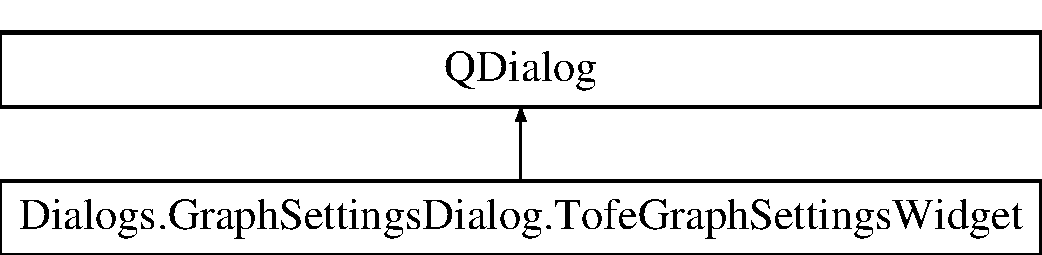
\includegraphics[height=2.000000cm]{classDialogs_1_1GraphSettingsDialog_1_1TofeGraphSettingsWidget}
\end{center}
\end{figure}
\subsection*{Public Member Functions}
\begin{DoxyCompactItemize}
\item 
def \hyperlink{classDialogs_1_1GraphSettingsDialog_1_1TofeGraphSettingsWidget_a3bf85acfd88552df3e5c0bcc781da6a1}{\-\_\-\-\_\-init\-\_\-\-\_\-}
\item 
def \hyperlink{classDialogs_1_1GraphSettingsDialog_1_1TofeGraphSettingsWidget_a20bf2ad6e8c2311fabc2f6a7c1de4fec}{accept\-\_\-settings}
\end{DoxyCompactItemize}
\subsection*{Public Attributes}
\begin{DoxyCompactItemize}
\item 
\hypertarget{classDialogs_1_1GraphSettingsDialog_1_1TofeGraphSettingsWidget_a32db939ed1252aec5501d126fcca466c}{{\bfseries parent}}\label{classDialogs_1_1GraphSettingsDialog_1_1TofeGraphSettingsWidget_a32db939ed1252aec5501d126fcca466c}

\item 
\hypertarget{classDialogs_1_1GraphSettingsDialog_1_1TofeGraphSettingsWidget_af2fd93cb001971f26588e38b0a1afaab}{{\bfseries ui}}\label{classDialogs_1_1GraphSettingsDialog_1_1TofeGraphSettingsWidget_af2fd93cb001971f26588e38b0a1afaab}

\end{DoxyCompactItemize}


\subsection{Detailed Description}
\begin{DoxyVerb}Graph settings dialog for the ToF-E histogram graph.
\end{DoxyVerb}
 

\subsection{Constructor \& Destructor Documentation}
\hypertarget{classDialogs_1_1GraphSettingsDialog_1_1TofeGraphSettingsWidget_a3bf85acfd88552df3e5c0bcc781da6a1}{\index{Dialogs\-::\-Graph\-Settings\-Dialog\-::\-Tofe\-Graph\-Settings\-Widget@{Dialogs\-::\-Graph\-Settings\-Dialog\-::\-Tofe\-Graph\-Settings\-Widget}!\-\_\-\-\_\-init\-\_\-\-\_\-@{\-\_\-\-\_\-init\-\_\-\-\_\-}}
\index{\-\_\-\-\_\-init\-\_\-\-\_\-@{\-\_\-\-\_\-init\-\_\-\-\_\-}!Dialogs::GraphSettingsDialog::TofeGraphSettingsWidget@{Dialogs\-::\-Graph\-Settings\-Dialog\-::\-Tofe\-Graph\-Settings\-Widget}}
\subsubsection[{\-\_\-\-\_\-init\-\_\-\-\_\-}]{\setlength{\rightskip}{0pt plus 5cm}def Dialogs.\-Graph\-Settings\-Dialog.\-Tofe\-Graph\-Settings\-Widget.\-\_\-\-\_\-init\-\_\-\-\_\- (
\begin{DoxyParamCaption}
\item[{}]{self, }
\item[{}]{parent}
\end{DoxyParamCaption}
)}}\label{classDialogs_1_1GraphSettingsDialog_1_1TofeGraphSettingsWidget_a3bf85acfd88552df3e5c0bcc781da6a1}
\begin{DoxyVerb}Inits ToF-E graph histogram graph settings dialog.

Args:
    parent: MatplotlibHistogramWidget which settings are being changed.
\end{DoxyVerb}
 

\subsection{Member Function Documentation}
\hypertarget{classDialogs_1_1GraphSettingsDialog_1_1TofeGraphSettingsWidget_a20bf2ad6e8c2311fabc2f6a7c1de4fec}{\index{Dialogs\-::\-Graph\-Settings\-Dialog\-::\-Tofe\-Graph\-Settings\-Widget@{Dialogs\-::\-Graph\-Settings\-Dialog\-::\-Tofe\-Graph\-Settings\-Widget}!accept\-\_\-settings@{accept\-\_\-settings}}
\index{accept\-\_\-settings@{accept\-\_\-settings}!Dialogs::GraphSettingsDialog::TofeGraphSettingsWidget@{Dialogs\-::\-Graph\-Settings\-Dialog\-::\-Tofe\-Graph\-Settings\-Widget}}
\subsubsection[{accept\-\_\-settings}]{\setlength{\rightskip}{0pt plus 5cm}def Dialogs.\-Graph\-Settings\-Dialog.\-Tofe\-Graph\-Settings\-Widget.\-accept\-\_\-settings (
\begin{DoxyParamCaption}
\item[{}]{self}
\end{DoxyParamCaption}
)}}\label{classDialogs_1_1GraphSettingsDialog_1_1TofeGraphSettingsWidget_a20bf2ad6e8c2311fabc2f6a7c1de4fec}
\begin{DoxyVerb}Accept changed settings and save them.
\end{DoxyVerb}
 

The documentation for this class was generated from the following file\-:\begin{DoxyCompactItemize}
\item 
Dialogs/Graph\-Settings\-Dialog.\-py\end{DoxyCompactItemize}

\hypertarget{classWidgets_1_1TofeHistogramWidget_1_1TofeHistogramWidget}{\section{Widgets.\-Tofe\-Histogram\-Widget.\-Tofe\-Histogram\-Widget Class Reference}
\label{classWidgets_1_1TofeHistogramWidget_1_1TofeHistogramWidget}\index{Widgets.\-Tofe\-Histogram\-Widget.\-Tofe\-Histogram\-Widget@{Widgets.\-Tofe\-Histogram\-Widget.\-Tofe\-Histogram\-Widget}}
}
Inheritance diagram for Widgets.\-Tofe\-Histogram\-Widget.\-Tofe\-Histogram\-Widget\-:\begin{figure}[H]
\begin{center}
\leavevmode
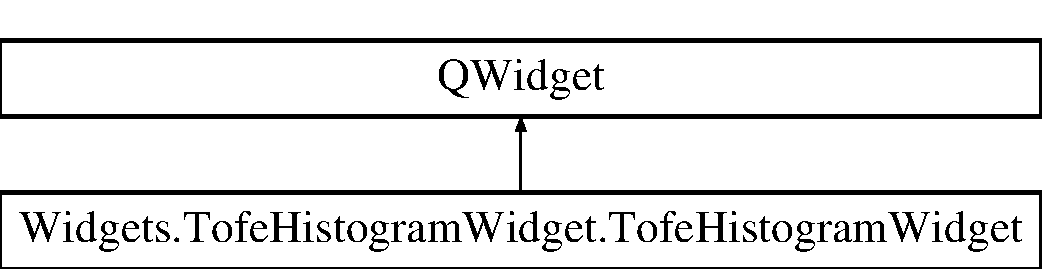
\includegraphics[height=2.000000cm]{classWidgets_1_1TofeHistogramWidget_1_1TofeHistogramWidget}
\end{center}
\end{figure}
\subsection*{Public Member Functions}
\begin{DoxyCompactItemize}
\item 
def \hyperlink{classWidgets_1_1TofeHistogramWidget_1_1TofeHistogramWidget_ae62599e21addfb4b00ef6307d20a404e}{\-\_\-\-\_\-init\-\_\-\-\_\-}
\item 
def \hyperlink{classWidgets_1_1TofeHistogramWidget_1_1TofeHistogramWidget_acd6f871c8e017a45c9711663c42db92f}{set\-\_\-cut\-\_\-button\-\_\-enabled}
\end{DoxyCompactItemize}
\subsection*{Public Attributes}
\begin{DoxyCompactItemize}
\item 
\hypertarget{classWidgets_1_1TofeHistogramWidget_1_1TofeHistogramWidget_ac79de3569efc186c342fb3bb9dea4029}{{\bfseries ui}}\label{classWidgets_1_1TofeHistogramWidget_1_1TofeHistogramWidget_ac79de3569efc186c342fb3bb9dea4029}

\item 
\hypertarget{classWidgets_1_1TofeHistogramWidget_1_1TofeHistogramWidget_a4ad66273da0a78469aad735f9af33b86}{{\bfseries measurement}}\label{classWidgets_1_1TofeHistogramWidget_1_1TofeHistogramWidget_a4ad66273da0a78469aad735f9af33b86}

\item 
\hypertarget{classWidgets_1_1TofeHistogramWidget_1_1TofeHistogramWidget_a3f01eba165e5e48e53cfdebde1396a68}{{\bfseries matplotlib}}\label{classWidgets_1_1TofeHistogramWidget_1_1TofeHistogramWidget_a3f01eba165e5e48e53cfdebde1396a68}

\end{DoxyCompactItemize}


\subsection{Detailed Description}
\begin{DoxyVerb}HistogramWidget used to draw ToF-E Histograms.
\end{DoxyVerb}
 

\subsection{Constructor \& Destructor Documentation}
\hypertarget{classWidgets_1_1TofeHistogramWidget_1_1TofeHistogramWidget_ae62599e21addfb4b00ef6307d20a404e}{\index{Widgets\-::\-Tofe\-Histogram\-Widget\-::\-Tofe\-Histogram\-Widget@{Widgets\-::\-Tofe\-Histogram\-Widget\-::\-Tofe\-Histogram\-Widget}!\-\_\-\-\_\-init\-\_\-\-\_\-@{\-\_\-\-\_\-init\-\_\-\-\_\-}}
\index{\-\_\-\-\_\-init\-\_\-\-\_\-@{\-\_\-\-\_\-init\-\_\-\-\_\-}!Widgets::TofeHistogramWidget::TofeHistogramWidget@{Widgets\-::\-Tofe\-Histogram\-Widget\-::\-Tofe\-Histogram\-Widget}}
\subsubsection[{\-\_\-\-\_\-init\-\_\-\-\_\-}]{\setlength{\rightskip}{0pt plus 5cm}def Widgets.\-Tofe\-Histogram\-Widget.\-Tofe\-Histogram\-Widget.\-\_\-\-\_\-init\-\_\-\-\_\- (
\begin{DoxyParamCaption}
\item[{}]{self, }
\item[{}]{measurement, }
\item[{}]{masses, }
\item[{}]{icon\-\_\-manager}
\end{DoxyParamCaption}
)}}\label{classWidgets_1_1TofeHistogramWidget_1_1TofeHistogramWidget_ae62599e21addfb4b00ef6307d20a404e}
\begin{DoxyVerb}Inits TofeHistogramWidget widget.

Args:
    measurement: A measurement class object.
    masses: A masses class object.
    icon_manager: An iconmanager class object.
\end{DoxyVerb}
 

\subsection{Member Function Documentation}
\hypertarget{classWidgets_1_1TofeHistogramWidget_1_1TofeHistogramWidget_acd6f871c8e017a45c9711663c42db92f}{\index{Widgets\-::\-Tofe\-Histogram\-Widget\-::\-Tofe\-Histogram\-Widget@{Widgets\-::\-Tofe\-Histogram\-Widget\-::\-Tofe\-Histogram\-Widget}!set\-\_\-cut\-\_\-button\-\_\-enabled@{set\-\_\-cut\-\_\-button\-\_\-enabled}}
\index{set\-\_\-cut\-\_\-button\-\_\-enabled@{set\-\_\-cut\-\_\-button\-\_\-enabled}!Widgets::TofeHistogramWidget::TofeHistogramWidget@{Widgets\-::\-Tofe\-Histogram\-Widget\-::\-Tofe\-Histogram\-Widget}}
\subsubsection[{set\-\_\-cut\-\_\-button\-\_\-enabled}]{\setlength{\rightskip}{0pt plus 5cm}def Widgets.\-Tofe\-Histogram\-Widget.\-Tofe\-Histogram\-Widget.\-set\-\_\-cut\-\_\-button\-\_\-enabled (
\begin{DoxyParamCaption}
\item[{}]{self, }
\item[{}]{selections = {\ttfamily None}}
\end{DoxyParamCaption}
)}}\label{classWidgets_1_1TofeHistogramWidget_1_1TofeHistogramWidget_acd6f871c8e017a45c9711663c42db92f}
\begin{DoxyVerb}Enables save cuts button if the given selections list's length is not 0.
Otherwise disable.

Args:
    selections: list of Selection objects
\end{DoxyVerb}
 

The documentation for this class was generated from the following file\-:\begin{DoxyCompactItemize}
\item 
Widgets/Tofe\-Histogram\-Widget.\-py\end{DoxyCompactItemize}

%--- End generated contents ---

% Index
\newpage
\phantomsection
\addcontentsline{toc}{part}{Index}
\printindex

\end{document}
